% Options for packages loaded elsewhere
\PassOptionsToPackage{unicode}{hyperref}
\PassOptionsToPackage{hyphens}{url}
%
\documentclass[
]{book}
\usepackage{lmodern}
\usepackage{amssymb,amsmath}
\usepackage{ifxetex,ifluatex}
\ifnum 0\ifxetex 1\fi\ifluatex 1\fi=0 % if pdftex
  \usepackage[T1]{fontenc}
  \usepackage[utf8]{inputenc}
  \usepackage{textcomp} % provide euro and other symbols
\else % if luatex or xetex
  \usepackage{unicode-math}
  \defaultfontfeatures{Scale=MatchLowercase}
  \defaultfontfeatures[\rmfamily]{Ligatures=TeX,Scale=1}
\fi
% Use upquote if available, for straight quotes in verbatim environments
\IfFileExists{upquote.sty}{\usepackage{upquote}}{}
\IfFileExists{microtype.sty}{% use microtype if available
  \usepackage[]{microtype}
  \UseMicrotypeSet[protrusion]{basicmath} % disable protrusion for tt fonts
}{}
\makeatletter
\@ifundefined{KOMAClassName}{% if non-KOMA class
  \IfFileExists{parskip.sty}{%
    \usepackage{parskip}
  }{% else
    \setlength{\parindent}{0pt}
    \setlength{\parskip}{6pt plus 2pt minus 1pt}}
}{% if KOMA class
  \KOMAoptions{parskip=half}}
\makeatother
\usepackage{xcolor}
\IfFileExists{xurl.sty}{\usepackage{xurl}}{} % add URL line breaks if available
\IfFileExists{bookmark.sty}{\usepackage{bookmark}}{\usepackage{hyperref}}
\hypersetup{
  pdftitle={Kinematik und Dynamik},
  pdfauthor={Kasel Ben},
  hidelinks,
  pdfcreator={LaTeX via pandoc}}
\urlstyle{same} % disable monospaced font for URLs
\usepackage{longtable,booktabs}
% Correct order of tables after \paragraph or \subparagraph
\usepackage{etoolbox}
\makeatletter
\patchcmd\longtable{\par}{\if@noskipsec\mbox{}\fi\par}{}{}
\makeatother
% Allow footnotes in longtable head/foot
\IfFileExists{footnotehyper.sty}{\usepackage{footnotehyper}}{\usepackage{footnote}}
\makesavenoteenv{longtable}
\usepackage{graphicx}
\makeatletter
\def\maxwidth{\ifdim\Gin@nat@width>\linewidth\linewidth\else\Gin@nat@width\fi}
\def\maxheight{\ifdim\Gin@nat@height>\textheight\textheight\else\Gin@nat@height\fi}
\makeatother
% Scale images if necessary, so that they will not overflow the page
% margins by default, and it is still possible to overwrite the defaults
% using explicit options in \includegraphics[width, height, ...]{}
\setkeys{Gin}{width=\maxwidth,height=\maxheight,keepaspectratio}
% Set default figure placement to htbp
\makeatletter
\def\fps@figure{htbp}
\makeatother
\setlength{\emergencystretch}{3em} % prevent overfull lines
\providecommand{\tightlist}{%
  \setlength{\itemsep}{0pt}\setlength{\parskip}{0pt}}
\setcounter{secnumdepth}{5}
\usepackage{booktabs}
\usepackage{tcolorbox}
\newenvironment{section-div}{}{}
\newenvironment{interactive}{}{}
\newenvironment{unnumbered}{}{}
\newenvironment{os-embed}{}{}
\newenvironment{learning-objectives}{}{}
\newenvironment{problems-exercises}{}{}
\newenvironment{conceptual-questions}{}{}
\newenvironment{section-summary}{}{}
%\newenvironment{glossary}{}{}
\newenvironment{test-prep-for-ap-courses}{}{}
\newenvironment{ap-test-prep}{}{}
\newenvironment{tinysection}{}{}
\newenvironment{note}{}{}


\usepackage[]{natbib}
\bibliographystyle{apalike}

\title{Kinematik und Dynamik}
\author{Kasel Ben}
\date{2020-07-06}

\begin{document}
\maketitle

{
\setcounter{tocdepth}{1}
\tableofcontents
}
\hypertarget{vorwort}{%
\chapter{Vorwort}\label{vorwort}}

Dieses Kapitel basiert auf der Arbeit von Openstax \citet{wolfe_college_2015} und wurde von Ben Kasel übersetzt und an das luxemburgische Schulsystem angepasst.

\hypertarget{kinematik}{%
\chapter{Kinematik}\label{kinematik}}

\hypertarget{einleitung}{%
\section{Einleitung}\label{einleitung}}

\begin{figure}
\hypertarget{import-auto-id2758213}{%
\centering
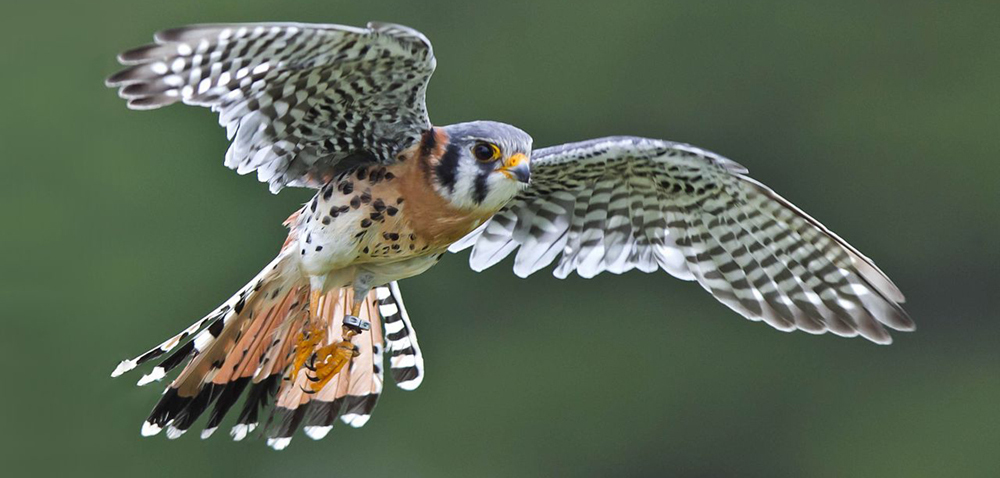
\includegraphics{images/Figure_02_00_01_D.jpg}
\caption{Die Bewegung eines Falken durch die Luft kann mit der Position, Geschwindigkeit und Beschleunigung des Vogels beschrieben werden. Bewegt er sich geradlinig, spricht man von einer ein-dimensionalen Bewegung. (credit: Vince Maidens, Wikimedia
Commons)}\label{import-auto-id2758213}
}
\end{figure}

Wo man auch hinsieht, beobachtet man Körper in Bewegung, von einem Tennismatch zum Vorbeiflug einer Raumsonde am Neptun. Selbst wenn man ruhig sitzt, bewegt das Herz Blut durch unsere Blutgefässe und jedes einzelne Atom und Molekül vibriert und bewegt sich kontinuierlich. Welche Fragen könnte man sich zu Bewegungen stellen? \emph{Wann wird eine bestimmte Raumsonde den Mars erreichen? Wie fliegt ein Fussball wenn er in einem bestimmten Winkel getreten wird?}

Die Analyse von Bewegungen liefert uns nicht nur Antworten auf diese Fragen, sondern bildet auch die Grundlage für weiterführende Konzepte in der Physik. So kann man \emph{Kräfte} nur schwer begreifen wenn man das Konzept der \emph{Beschleunigung} nicht versteht. Diese Verbindung zwischen Kräften und Beschleunigung ist nötig um die \emph{Grundidee 3} zu verstehen.

Um Bewegungen quantitativ zu beschreibungen, wird in dieser Einheit das Thema des \emph{Bezugsystems} behandelt. Wenn Sie bereits von einer Freundin am Bahnhofsteig verabschiedet haben, verstehen Sie diese Idee bestimmt. Sie sehen wie Ihre Freundin sich von Ihnen entfernt, obwohl sie sich für die anderen Passagiere im Ruhezustand befindet. Das Bezugsystem beeinflusst die Beobachtung und dieser Zusammenhang muss für ein grundlegendes Verständnis von 3.A und Essential Knowledge 3.A.1. klar sein.

Das formale Studium der Physik beginnt mit der \textbf{Kinematik} die als \emph{Lehre der Bewegung ohne deren Ursachen} definiert ist. Man untersucht also zum Beispiel die ein- oder zwei-dimensionale Bewegung eines Fussballs ohne sich zu Fragen welche Kräfte die Bewegung verursacht haben. In diesem Kapitel beschränken wir uns auf die einfachsten Bewegungen, solche die eindimensional oder geradlinig sind. Die gelernten Konzepte wenden wir dann im nächsten Kapitel auf Bewegungen mit kurvenförmigen Bahnkurven oder zweidimensionale Bewegungen an, zum Beispiel ein Auto in einer Kurve.

Der Inhalt dieses Kapitels unterstützt

\textbf{Grundidee 3} Wechselwirkungen zwischen Körpern können mit Kräften beschrieben werden.

\emph{dauerhaftes Verständnis 3.A} Beobachter in Inertialsystemen sind sich einig über die Charakteristiken von Kräften.

\emph{Essential Knowledge 3.A.1} Ein Beobachter in einem bestimmten Bezugsystem kann die Bewegung eines Körpers andhand der Grössen Position, Positionsänderung, Strecke, Geschwindigkeit (Vektor oder Betrag) und Beschleunigung beschreiben.

\hypertarget{concept-trailer-1d-kinematics}{}

\hypertarget{positionsuxe4nderung}{%
\section{Positionsänderung}\label{positionsuxe4nderung}}

\begin{figure}
\hypertarget{import-auto-id2723149}{%
\centering
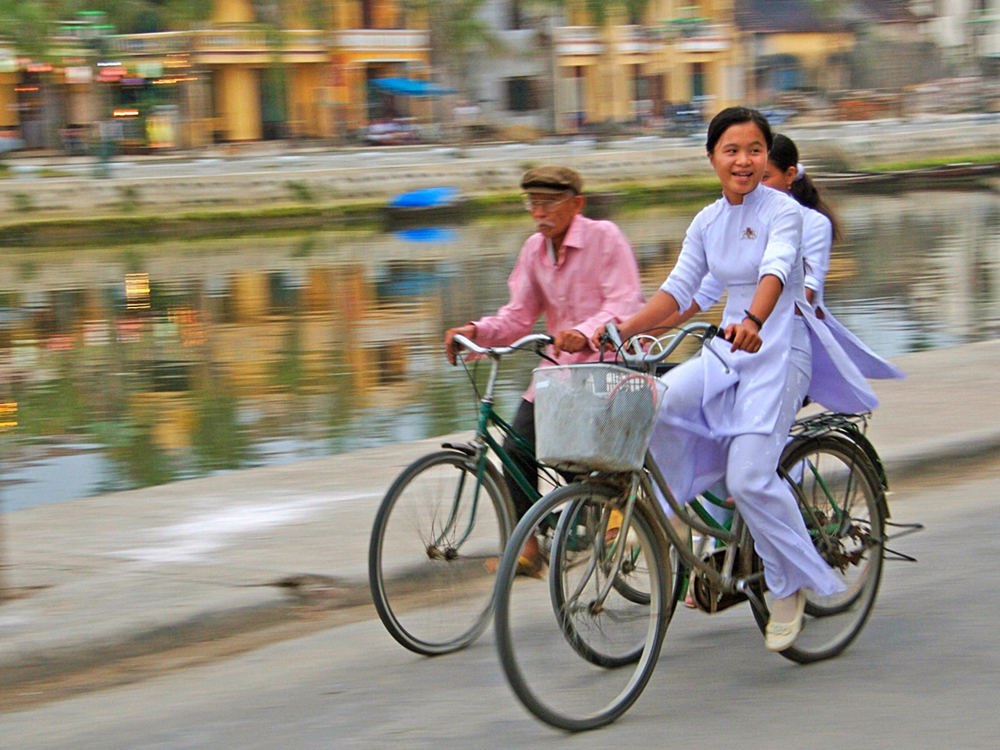
\includegraphics{images/Figure_02_01_00.jpg}
\caption{Diese Fahrradfahrer in Vietnam können anhand ihrer Position in Bezug auf die Gebäude oder den Kanal beschrieben werden. Ihre Bewegung kann mit der Änderung der Position in diesem Bezugsystem beschrieben werden. (credit: Suzan
Black, Fotopedia)}\label{import-auto-id2723149}
}
\end{figure}

\hypertarget{fs-id3277370}{}
\begin{learning-objectives}

\hypertarget{lernziele}{%
\subsection{Lernziele}\label{lernziele}}

Nach diesem Kapitel solltest du folgendes können:

\begin{itemize}
\tightlist
\item
  Position, Positionsänderung, Strecke, zurückgelegte Strecke in einem bestimmten Bezugsystem definieren.
\item
  Den Zusammenhang zwischen Possition und Positionsänderung erklären.
\item
  Den Unterschied zwischen Positionsänderung und zurückgelegter Strecke kennen.
\item
  Die Positionsänderung, und Strecke anhand der Anfangs- und Endposition, sowie der Bahnkurve zwischen beiden Punkten
\end{itemize}

Die Informationen in diesem Kapitel unterstützen folgende Punkte des AP® Kurriculums:

\begin{itemize}
\tightlist
\item
  \textbf{3.A.1.1} Der Schüler kann die Bewegung eines Körpers sprachlich, mathematisch und und grafisch beschreiben.
  \textbf{(S.P. 1.5, 2.1, 2.2)}
\item
  \textbf{3.A.1.3} Der Schüler kann Versuchsergebnisse analysieren und diese dazu nutzen die Bewegung des untersuchten Körpers sprachlich, mathematisch und grafisch darstellen. \textbf{(S.P. 5.1)}
\end{itemize}

\end{learning-objectives}

\hypertarget{fs-id3178358}{}
\hypertarget{position}{%
\subsection{Position}\label{position}}

Bovir man sich der Beschreibung der Bewegung widmen kann, muss man zuvor die {Position} oder den Ort eines Körpers zu einem bestimmten Zeitpunkt zu bestimmen --- Wo befindet sich der Körper, oder genauer gefragt, wo im Bezug zu einem bestimmten Beobachter. Die Erde wird oft als Bezugsystem benutzt und wir beschreiben die Bewegung eines Körpers in Bezug auf Körper die in diesem Bezugsystem ruhen. Zum Beispiel wird der Start einer Rakete in Bezug auf die gesamte Erde beschrieben, während die Position des Lehrers in Bezug auf die Tafel beschrieben wird. (Abbildung
\citet{ref}\{import-auto-id2972079\} \protect\hyperlink{import-auto-id2972079}{link}.) In other cases,
we use reference frames that are not stationary but are in motion
relative to the Earth. To describe the position of a person in an
airplane, for example, we use the airplane, not the Earth, as the
reference frame. (See
\protect\hyperlink{import-auto-id2707699}{link}.)

\hypertarget{fs-id2572460}{}
\hypertarget{displacement-1}{%
\subsection{Displacement}\label{displacement-1}}

If an object moves relative to a reference frame (for example, if a
professor moves to the right relative to a white board or a passenger
moves toward the rear of an airplane), then the object's position
changes. This change in position is known as
{displacement}. The word ``displacement'' implies that
an object has moved, or has been displaced.

\hypertarget{fs-id3206000}{}
\begin{note}

Displacement

Displacement is the \emph{change in position} of an object:

\leavevmode\hypertarget{eip-458}{}%
\[{\text{Δ}x = {x_{\text{f}} - x_{0}},}{}\]

where \({\text{Δ}x}{}\) is displacement, \(x_{\text{f}}{}\) is the final
position, and \emph{}\(x_{0}{}\) is the initial
position.

\end{note}

In this text the upper case Greek letter \(\text{Δ}{}\) (delta) always
means ``change in'' whatever quantity follows it; thus, \({\text{Δ}x}{}\)
means \emph{change in position}. Always solve for displacement by subtracting
initial position \(x_{0}{}\) from final position \(x_{\text{f}}{}\).

Note that the SI unit for displacement is the meter (m) (see \href{/m54765}{Physical
Quantities and Units}), but sometimes kilometers, miles, feet,
and other units of length are used. Keep in mind that when units other
than the meter are used in a problem, you may need to convert them into
meters to complete the calculation.

\begin{figure}
\hypertarget{import-auto-id2972079}{%
\centering
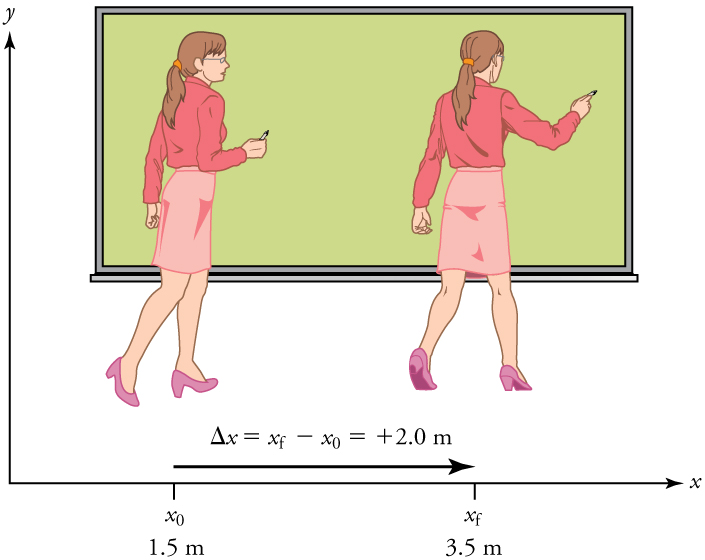
\includegraphics{images/Figure_02_01_01.jpg}
\caption{A professor paces left and right while lecturing. Her position
relative to the blackboard is given by \(x{}\). The
\({{+ 2}\text{.}0\ \text{m}}{}\) displacement of the professor relative to
the blackboard is represented by an arrow pointing to the
right.}\label{import-auto-id2972079}
}
\end{figure}

\begin{figure}
\hypertarget{import-auto-id2707699}{%
\centering
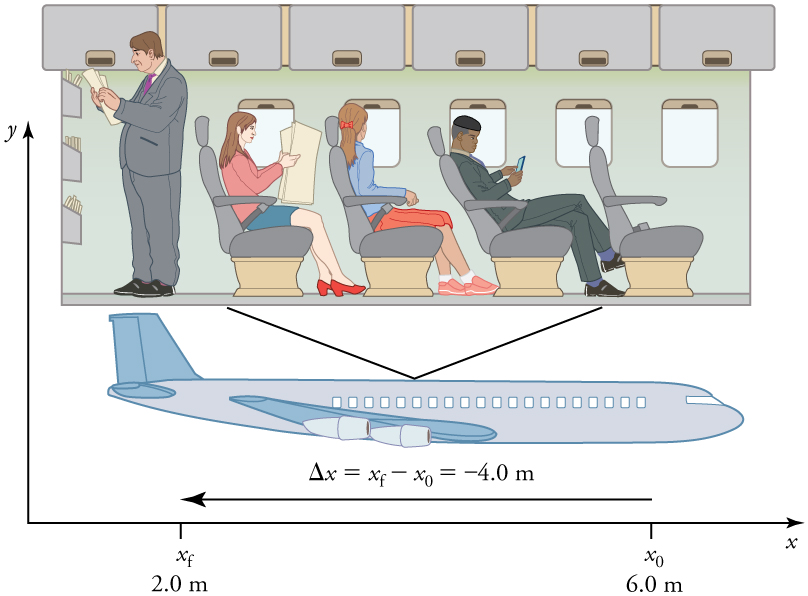
\includegraphics{images/Figure 02_01_02.jpg}
\caption{A passenger moves from his seat to the back of the plane. His location
relative to the airplane is given by \(x{}\). The −4 m displacement of the
passenger relative to the plane is represented by an arrow toward the
rear of the plane. Notice that the arrow representing his displacement
is twice as long as the arrow representing the displacement of the
professor (he moves twice as far) in
\protect\hyperlink{import-auto-id2972079}{link}.}\label{import-auto-id2707699}
}
\end{figure}

Note that displacement has a direction as well as a magnitude. The
professor's displacement is 2.0 m to the right, and the airline
passenger's displacement is 4.0 m toward the rear. In one-dimensional
motion, direction can be specified with a plus or minus sign. When you
begin a problem, you should select which direction is positive (usually
that will be to the right or up, but you are free to select positive as
being any direction). The professor's initial position is
\({{x_{0} = 1}\text{.}5\ \text{m}}{}\) and her final position is
\({{x_{\text{f}} = 3}\text{.}5\ \text{m}}{}\). Thus her displacement is

\leavevmode\hypertarget{eip-556}{}%
\[{{{\Delta x = x_{f}{- x_{0}} = 3}\text{.5\ m} - 1.5\ m = + 2\text{.0\ m}}.}{}\]

In this coordinate system, motion to the right is positive, whereas
motion to the left is negative. Similarly, the airplane passenger's
initial position is \({x_{0} = 6}\text{.}0\ m\) and his final position is
\({{x_{f} = 2}\text{.}0\ m}{}\), so his displacement is

\leavevmode\hypertarget{eip-778}{}%
\[{{\Delta x = x_{f}{- x_{0}} = 2}\text{.}0\ m - 6\text{.}0\ m = {- 4}\text{.}0\ m}.\]

His displacement is negative because his motion is toward the rear of
the plane, or in the negative \(x{}\) direction in our coordinate system.

\hypertarget{fs-id1414454}{}
\hypertarget{distance}{%
\subsection{Distance}\label{distance}}

Although displacement is described in terms of direction, distance is
not. {Distance} is defined to be \emph{the magnitude or
size of displacement between two positions}. Note that the distance
between two positions is not the same as the distance traveled between
them. {Distance traveled} is \emph{the total length of the
path traveled between two positions}. Distance has no direction and,
thus, no sign. For example, the distance the professor walks is 2.0 m.
The distance the airplane passenger walks is 4.0 m.

\hypertarget{fs-id3044492}{}
\begin{note}

Misconception Alert: Distance Traveled vs.~Magnitude of Displacement

It is important to note that the \emph{distance traveled},
\emph{}however, can be greater than the
magnitude of the displacement (by magnitude, we mean just the size of
the displacement without regard to its direction; that is, just a number
with a unit). For example, the professor could pace back and forth many
times, perhaps walking a distance of 150 m during a lecture, yet still
end up only 2.0 m to the right of her starting point. In this case her
displacement would be +2.0 m, the magnitude of her displacement would be
2.0 m, but the distance she traveled would be 150 m. In kinematics we
nearly always deal with displacement and magnitude of displacement, and
almost never with distance traveled. One way to think about this is to
assume you marked the start of the motion and the end of the motion. The
displacement is simply the difference in the position of the two marks
and is independent of the path taken in traveling between the two marks.
The distance traveled, however, is the total length of the path taken
between the two marks.

\end{note}

\hypertarget{fs-id3589986}{}
Check Your Understanding

\leavevmode\hypertarget{fs-id2996632}{}%
A cyclist rides 3 km west and then turns around and rides 2 km east. (a)
What is her displacement? (b) What distance does she ride? (c) What is
the magnitude of her displacement?

\leavevmode\hypertarget{fs-id1711333}{}%
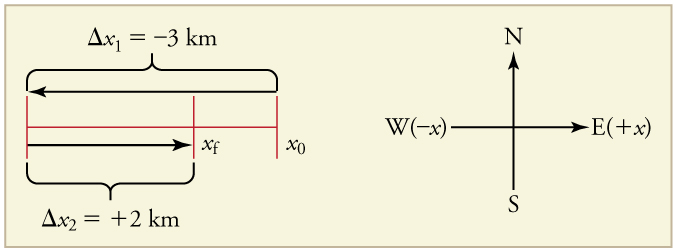
\includegraphics{images/Figure_02_01_03.jpg}

\(a\) The rider's displacement is
\({{\Delta x = {x_{f} - x_{0}}} = \text{−1\ km}}{}\). (The displacement is
negative because we take east to be positive and west to be negative.)

\(b\) The distance traveled is
\({{\text{3\ km} + \text{2\ km}} = \text{5\ km}}{}\).

\(c\) The magnitude of the displacement is \(1\ km{}\).

\hypertarget{fs-id2758854-summary}{}
\hypertarget{section-summary}{%
\subsection{Section Summary}\label{section-summary}}

\begin{itemize}
\item
  Kinematics is the study of motion without considering its causes. In
  this chapter, it is limited to motion along a straight line, called
  one-dimensional motion.
\item
  Displacement is the change in position of an object.
\item
  In symbols, displacement \({\Delta x}{}\) is defined to be
  ::: \{\#fs-id2929393 data-type=``equation''\}
  \[{\Delta x = {x_{f} - x_{0}},}{}\]

  :::

  where \(x_{0}\) is the initial position and \(x_{f}{}\) is the final
  position. In this text, the Greek letter \(\Delta{}\) (delta) always
  means ``change in'' whatever quantity follows it. The SI unit for
  displacement is the meter (m). Displacement has a direction as well
  as a magnitude.
\item
  When you start a problem, assign which direction will be positive.
\item
  Distance is the magnitude of displacement between two positions.
\item
  Distance traveled is the total length of the path traveled between
  two positions.
\end{itemize}

\hypertarget{fs-id2075470}{}
\begin{conceptual-questions}

\hypertarget{conceptual-questions}{%
\subsection{Conceptual Questions}\label{conceptual-questions}}

\hypertarget{fs-id1704056}{}
\leavevmode\hypertarget{fs-id1942381}{}%
Give an example in which there are clear distinctions among distance
traveled, displacement, and magnitude of displacement. Specifically
identify each quantity in your example.

\hypertarget{fs-id3147584}{}
\leavevmode\hypertarget{fs-id1702540}{}%
Under what circumstances does distance traveled equal magnitude of
displacement? What is the only case in which magnitude of displacement
and distance are exactly the same?

\hypertarget{fs-id3563423}{}
\leavevmode\hypertarget{fs-id2781126}{}%
Bacteria move back and forth by using their flagella (structures that
look like little tails). Speeds of up to
\({\text{50\ μm/s}\ \left( {{\text{50} \times \text{10}^{- 6}}\ \text{m/s}} \right)}{}\)
have been observed. The total distance traveled by a bacterium is large
for its size, while its displacement is small. Why is this?

\end{conceptual-questions}

\hypertarget{fs-id3417389}{}
\begin{problems-exercises}

\hypertarget{problems-exercises}{%
\subsection{Problems \& Exercises}\label{problems-exercises}}

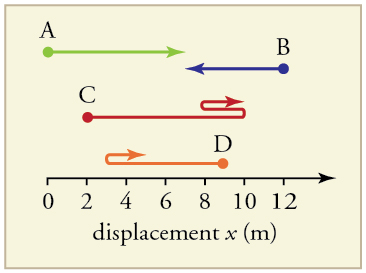
\includegraphics{images/Figure_02_01Sol_01.jpg}

\hypertarget{fs-id1126076}{}
\leavevmode\hypertarget{fs-id3312138}{}%
Find the following for path A in
\protect\hyperlink{import-auto-id2076702}{link}: (a) The distance
traveled. (b) The magnitude of the displacement from start to finish.
(c) The displacement from start to finish.

\leavevmode\hypertarget{fs-id1551519}{}%
\(a\) 7 m

\(b\) 7 m

\(c\) \({+ 7\ m}{}\)

\hypertarget{fs-id2823990}{}
\leavevmode\hypertarget{fs-id2804044}{}%
Find the following for path B in
\protect\hyperlink{import-auto-id2076702}{link}: (a) The distance
traveled. (b) The magnitude of the displacement from start to finish.
(c) The displacement from start to finish.

\hypertarget{fs-id4292134}{}
\leavevmode\hypertarget{fs-id2811336}{}%
Find the following for path C in
\protect\hyperlink{import-auto-id2076702}{link}: (a) The distance
traveled. (b) The magnitude of the displacement from start to finish.
(c) The displacement from start to finish.

\leavevmode\hypertarget{fs-id2791412}{}%
\(a\) 13 m

\(b\) 9 m

\(c\) \({+ 9\ m}{}\)

\hypertarget{fs-id3242594}{}
\leavevmode\hypertarget{fs-id1470371}{}%
Find the following for path D in
\protect\hyperlink{import-auto-id2076702}{link}: (a) The distance
traveled. (b) The magnitude of the displacement from start to finish.
(c) The displacement from start to finish.

\end{problems-exercises}

\hypertarget{fs-id1915464}{}
\begin{ap-test-prep}

\hypertarget{test-prep-for-ap-courses}{%
\subsection{Test Prep for AP Courses}\label{test-prep-for-ap-courses}}

\hypertarget{fs-id1862594}{}
\leavevmode\hypertarget{fs-id2378785}{}%
Which of the following statements comparing position, distance traveled,
and displacement is correct?

\begin{enumerate}
\def\labelenumi{\alph{enumi}.}
\tightlist
\item
  An object may record a distance traveled of zero while recording a
  non-zero displacement.
\item
  An object may record a non-zero distance traveled while recording a
  displacement of zero.
\item
  An object may record a non-zero distance traveled while maintaining
  a position of zero.
\item
  An object may record a non-zero displacement while maintaining a
  position of zero.
\end{enumerate}

\leavevmode\hypertarget{fs-id2165037}{}%
\(a\)

\end{ap-test-prep}

\hypertarget{glossary}{%
\subsection{Glossary}\label{glossary}}

\begin{description}
\tightlist
\item[kinematics]
the study of motion without considering its causes
\end{description}

\begin{description}
\tightlist
\item[position]
the location of an object at a particular time
\end{description}

\begin{description}
\tightlist
\item[displacement]
the change in position of an object
\end{description}

\begin{description}
\tightlist
\item[distance]
the magnitude of displacement between two positions
\end{description}

\begin{description}
\tightlist
\item[distance traveled]
the total length of the path traveled between two positions
\end{description}

\hypertarget{vectors-scalars-and-coordinate-systems}{%
\section{Vectors, Scalars, and Coordinate Systems}\label{vectors-scalars-and-coordinate-systems}}

\begin{figure}
\hypertarget{import-auto-id1778274}{%
\centering
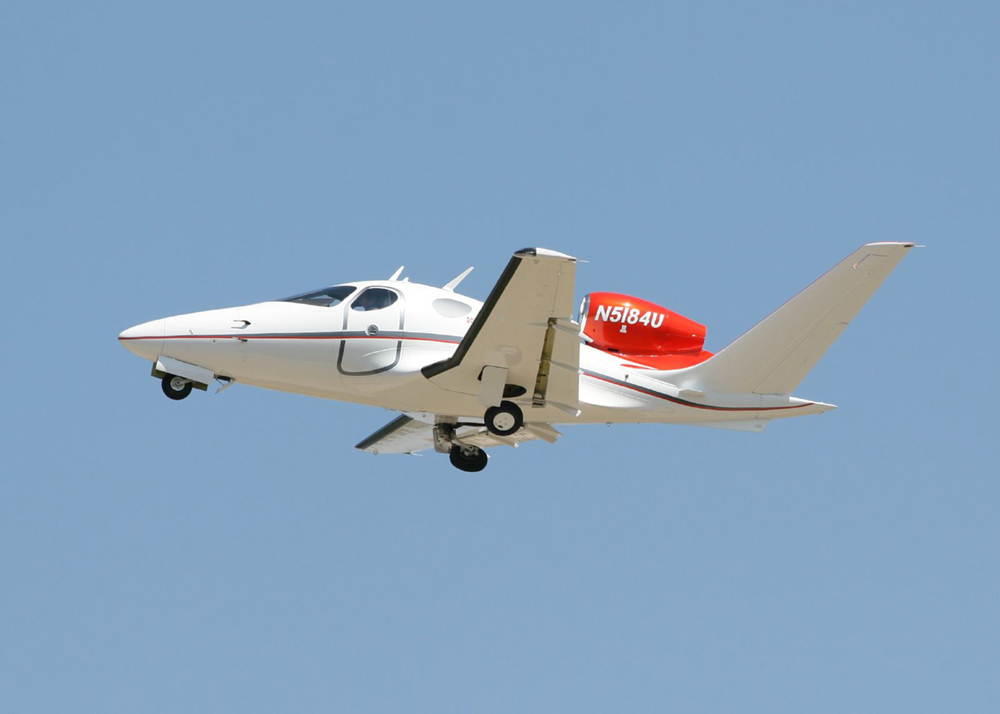
\includegraphics{images/Figure_02_02_00.jpg}
\caption{The motion of this Eclipse Concept jet can be described in terms of
the distance it has traveled (a scalar quantity) or its displacement in
a specific direction (a vector quantity). In order to specify the
direction of motion, its displacement must be described based on a
coordinate system. In this case, it may be convenient to choose motion
toward the left as positive motion (it is the forward direction for the
plane), although in many cases, the \(x{}\)-coordinate runs from left to
right, with motion to the right as positive and motion to the left as
negative. (credit: Armchair Aviator,
Flickr)}\label{import-auto-id1778274}
}
\end{figure}

\hypertarget{fs-id1545372}{}
\begin{learning-objectives}

\hypertarget{learning-objectives}{%
\subsection{Learning Objectives}\label{learning-objectives}}

By the end of this section, you will be able to:

\begin{itemize}
\tightlist
\item
  Define and distinguish between scalar and vector quantities.
\item
  Assign a coordinate system for a scenario involving one-dimensional
  motion.
\end{itemize}

The information presented in this section supports the following AP®
learning objectives and science practices:

\begin{itemize}
\tightlist
\item
  \textbf{3.A.1.2} The student is able to design an experimental
  investigation of the motion of an object.
\end{itemize}

\end{learning-objectives}

What is the difference between distance and displacement? Whereas
displacement is defined by both direction and magnitude, distance is
defined only by magnitude. Displacement is an example of a vector
quantity. Distance is an example of a scalar quantity. A
\protect\hypertarget{import-auto-id1738434}{}{vector} is any quantity with
both \emph{magnitude and direction}. Other examples of vectors include a
velocity of 90 km/h east and a force of 500 newtons straight down.

The direction of a vector in one-dimensional motion is given simply by a
plus \({( + )}{}\) or minus \({( - )}{}\) sign. Vectors are represented
graphically by arrows. An arrow used to represent a vector has a length
proportional to the vector's magnitude (e.g., the larger the magnitude,
the longer the length of the vector) and points in the same direction as
the vector.

Some physical quantities, like distance, either have no direction or
none is specified. A \protect\hypertarget{import-auto-id1759638}{}{scalar}
is any quantity that has a magnitude, but no direction. For example, a
\(\text{20ºC}\) temperature, the 250 kilocalories (250 Calories) of energy
in a candy bar, a 90 km/h speed limit, a person's 1.8 m height, and a
distance of 2.0 m are all scalars---quantities with no specified
direction. Note, however, that a scalar can be negative, such as a
\(- \text{20ºC}\) temperature. In this case, the minus sign indicates a
point on a scale rather than a direction. Scalars are never represented
by arrows.

\hypertarget{fs-id1655694}{}
\hypertarget{coordinate-systems-for-one-dimensional-motion}{%
\subsection{Coordinate Systems for One-Dimensional Motion}\label{coordinate-systems-for-one-dimensional-motion}}

In order to describe the direction of a vector quantity, you must
designate a coordinate system within the reference frame. For
one-dimensional motion, this is a simple coordinate system consisting of
a one-dimensional coordinate line. In general, when describing
horizontal motion, motion to the right is usually considered positive,
and motion to the left is considered negative. With vertical motion,
motion up is usually positive and motion down is negative. In some
cases, however, as with the jet in
\protect\hyperlink{import-auto-id1778274}{link}, it can be more
convenient to switch the positive and negative directions. For example,
if you are analyzing the motion of falling objects, it can be useful to
define downwards as the positive direction. If people in a race are
running to the left, it is useful to define left as the positive
direction. It does not matter as long as the system is clear and
consistent. Once you assign a positive direction and start solving a
problem, you cannot change it.

\begin{figure}
\hypertarget{import-auto-id1758074}{%
\centering
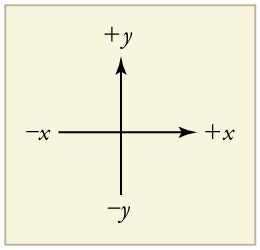
\includegraphics{images/Figure_02_02_00b.jpg}
\caption{It is usually convenient to consider motion upward or to the right as
positive \({( + )}{}\) and motion downward or to the left as negative
\({( - )}{}\).}\label{import-auto-id1758074}
}
\end{figure}

\hypertarget{fs-id1788025}{}
Check Your Understanding

\leavevmode\hypertarget{fs-id1765357}{}%
A person's speed can stay the same as he or she rounds a corner and
changes direction. Given this information, is speed a scalar or a vector
quantity? Explain.

\leavevmode\hypertarget{fs-id2007066}{}%
Speed is a scalar quantity. It does not change at all with direction
changes; therefore, it has magnitude only. If it were a vector quantity,
it would change as direction changes (even if its magnitude remained
constant).

\hypertarget{fs-id1784568-summary}{}
\hypertarget{section-summary-1}{%
\subsection{Section Summary}\label{section-summary-1}}

\begin{itemize}
\tightlist
\item
  \protect\hypertarget{import-auto-id1534176}{}{A vector is any quantity that has magnitude and
  direction.}
\item
  \protect\hypertarget{import-auto-id1777731}{}{A scalar is any quantity that has magnitude but no
  direction.}
\item
  \protect\hypertarget{import-auto-id1416292}{}{Displacement and velocity are vectors, whereas distance and speed
  are scalars.}
\item
  \protect\hypertarget{import-auto-id1739033}{}{In one-dimensional motion, direction is specified by a plus or
  minus sign to signify left or right, up or down, and the
  like.}
\end{itemize}

\hypertarget{fs-id1799980}{}
\begin{conceptual-questions}

\hypertarget{conceptual-questions-1}{%
\subsection{Conceptual Questions}\label{conceptual-questions-1}}

\hypertarget{fs-id1364975}{}
\leavevmode\hypertarget{fs-id1770280}{}%
A student writes, ``\emph{A bird that is diving for prey has a speed of}
\({- \textit{10}\ {m/s}}{}\).'' What is wrong with the student's
statement? What has the student actually described? Explain.

\hypertarget{fs-id1773292}{}
\leavevmode\hypertarget{fs-id1706742}{}%
What is the speed of the bird in
\protect\hyperlink{fs-id1364975}{link}?

\hypertarget{fs-id1247502}{}
\leavevmode\hypertarget{fs-id1777549}{}%
Acceleration is the change in velocity over time. Given this
information, is acceleration a vector or a scalar quantity? Explain.

\hypertarget{fs-id1548043}{}
\leavevmode\hypertarget{fs-id1778185}{}%
A weather forecast states that the temperature is predicted to be
\({- 5ºC}{}\) the following day. Is this temperature a vector or a scalar
quantity? Explain.

\end{conceptual-questions}

\hypertarget{fs-id2066209}{}
\begin{note}

Switching Reference Frames

A fundamental tenet of physics is that information about an event can be
gathered from a variety of reference frames. For example, imagine that
you are a passenger walking toward the front of a bus. As you walk, your
motion is observed by a fellow bus passenger and by an observer standing
on the sidewalk.

Both the bus passenger and sidewalk observer will be able to collect
information about you. They can determine how far you moved and how much
time it took you to do so. However, while you moved at a consistent
pace, both observers will get different results. To the passenger
sitting on the bus, you moved forward at what one would consider a
normal pace, something similar to how quickly you would walk outside on
a sunny day. To the sidewalk observer though, you will have moved much
quicker. Because the bus is also moving forward, the distance you move
forward against the sidewalk each second increases, and the sidewalk
observer must conclude that you are moving at a greater pace.

To show that you understand this concept, you will need to create an
event and think of a way to view this event from two different frames of
reference. In order to ensure that the event is being observed
simultaneously from both frames, you will need an assistant to help out.
An example of a possible event is to have a friend ride on a skateboard
while tossing a ball. How will your friend observe the ball toss, and
how will those observations be different from your own?

Your task is to describe your event and the observations of your event
from both frames of reference. Answer the following questions below to
demonstrate your understanding. For assistance, you can review the
information given in the 'Position' paragraph at the start of Section
2.1.

\begin{enumerate}
\def\labelenumi{\arabic{enumi}.}
\tightlist
\item
  What is your event? What object are both you and your assistant
  observing?
\item
  What do \emph{you} see as the event takes place?
\item
  What does \emph{your assistant} see as the event takes place?
\item
  How do your reference frames cause you and your assistant to have
  two different sets of observations?
\end{enumerate}

\end{note}

\hypertarget{fs-id1368980}{}
\begin{ap-test-prep}

\hypertarget{test-prep-for-ap-courses-1}{%
\subsection{Test Prep for AP Courses}\label{test-prep-for-ap-courses-1}}

\hypertarget{fs-id1890618}{}
\leavevmode\hypertarget{fs-id1408528}{}%
A student is trying to determine the acceleration of a feather as she
drops it to the ground. If the student is looking to achieve a positive
velocity and positive acceleration, what is the \emph{most sensible} way to
set up her coordinate system?

\begin{enumerate}
\def\labelenumi{\alph{enumi}.}
\tightlist
\item
  Her hand should be a coordinate of zero and the upward direction
  should be considered positive.
\item
  Her hand should be a coordinate of zero and the downward direction
  should be considered positive.
\item
  The floor should be a coordinate of zero and the upward direction
  should be considered positive.
\item
  The floor should be a coordinate of zero and the downward direction
  should be considered positive.
\end{enumerate}

\end{ap-test-prep}

\hypertarget{glossary-1}{%
\subsection{Glossary}\label{glossary-1}}

\begin{description}
\tightlist
\item[scalar]
a quantity that is described by magnitude, but not direction
\end{description}

\begin{description}
\tightlist
\item[vector]
a quantity that is described by both magnitude and direction
\end{description}

\hypertarget{time-velocity-and-speed}{%
\section{Time, Velocity, and Speed}\label{time-velocity-and-speed}}

\begin{figure}
\hypertarget{import-auto-id1690049}{%
\centering
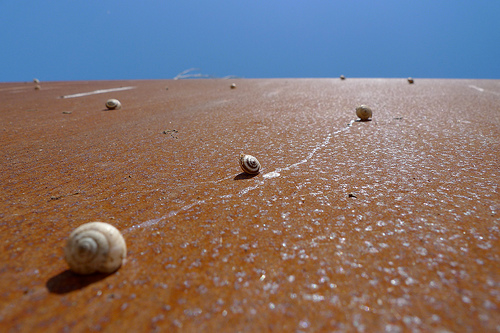
\includegraphics{images/Picture 6.png}
\caption{The motion of these racing snails can be described by their speeds and
their velocities. (credit: tobitasflickr,
Flickr)}\label{import-auto-id1690049}
}
\end{figure}

\hypertarget{fs-id1037368}{}
\begin{learning-objectives}

\hypertarget{learning-objectives-1}{%
\subsection{Learning Objectives}\label{learning-objectives-1}}

By the end of this section, you will be able to:

\begin{itemize}
\tightlist
\item
  Explain the relationships between instantaneous velocity, average
  velocity, instantaneous speed, average speed, displacement, and
  time.
\item
  Calculate velocity and speed given initial position, initial time,
  final position, and final time.
\item
  Derive a graph of velocity vs.~time given a graph of position vs.
  time.
\item
  Interpret a graph of velocity vs.~time.
\end{itemize}

The information presented in this section supports the following AP®
learning objectives and science practices:

\begin{itemize}
\tightlist
\item
  \textbf{3.A.1.1} The student is able to express the motion of an object
  using narrative, mathematical, and graphical representations.
  \textbf{(S.P. 1.5, 2.1, 2.2)}
\item
  \textbf{3.A.1.3} The student is able to analyze experimental data
  describing the motion of an object and is able to express the
  results of the analysis using narrative, mathematical, and graphical
  representations. \textbf{(S.P. 5.1)}
\end{itemize}

\end{learning-objectives}

There is more to motion than distance and displacement. Questions such
as, ``How long does a foot race take?'' and ``What was the runner's
speed?'' cannot be answered without an understanding of other concepts.
In this section we add definitions of time, velocity, and speed to
expand our description of motion.

\hypertarget{fs-id1568419}{}
\hypertarget{time}{%
\subsection{Time}\label{time}}

As discussed in \href{/m54765}{Physical Quantities and Units}, the most
fundamental physical quantities are defined by how they are measured.
This is the case with time. Every measurement of time involves measuring
a change in some physical quantity. It may be a number on a digital
clock, a heartbeat, or the position of the Sun in the sky. In physics,
the definition of time is simple---\protect\hypertarget{import-auto-id2588516}{}{time} is \emph{change}, or the interval over which change occurs.
It is impossible to know that time has passed unless something changes.

The amount of time or change is calibrated by comparison with a
standard. The SI unit for time is the second, abbreviated s. We might,
for example, observe that a certain pendulum makes one full swing every
0.75 s. We could then use the pendulum to measure time by counting its
swings or, of course, by connecting the pendulum to a clock mechanism
that registers time on a dial. This allows us to not only measure the
amount of time, but also to determine a sequence of events.

How does time relate to motion? We are usually interested in elapsed
time for a particular motion, such as how long it takes an airplane
passenger to get from his seat to the back of the plane. To find elapsed
time, we note the time at the beginning and end of the motion and
subtract the two. For example, a lecture may start at 11:00
\textsc{A.M.} and end at 11:50 \textsc{A.M.}, so that the
elapsed time would be 50 min. \protect\hypertarget{import-auto-id4083152}{}{Elapsed time} \textbf{\({\Delta t}{}\)} is the difference between the
ending time and beginning time,

\leavevmode\hypertarget{import-auto-id1757927}{}%
\[\Delta t = {t_{f} - t_{0}},\]

where \({\Delta t}{}\) is the change in time or elapsed time, \(t_{f}{}\) is
the time at the end of the motion, and \(t_{0}{}\) is the time at the
beginning of the motion. (As usual, the delta symbol, \(\Delta{}\), means
the change in the quantity that follows it.)

Life is simpler if the beginning time \(t_{0}{}\) is taken to be zero, as
when we use a stopwatch. If we were using a stopwatch, it would simply
read zero at the start of the lecture and 50 min at the end. If
\(t_{0} = 0\), then \({\Delta t = t_{f}} \equiv t\).

In this text, for simplicity's sake,

\begin{itemize}
\tightlist
\item
  \protect\hypertarget{import-auto-id2571110}{}{motion starts at time equal to zero
  \({({t_{0} = 0})}{}\)}
\item
  \protect\hypertarget{import-auto-id4047929}{}{the symbol \(t{}\) is used for elapsed time unless otherwise
  specified
  \({({{\Delta t = t_{f}} \equiv t})}{}\)}
\end{itemize}

\hypertarget{fs-id1850777}{}
\hypertarget{velocity}{%
\subsection{Velocity}\label{velocity}}

Your notion of velocity is probably the same as its scientific
definition. You know that if you have a large displacement in a small
amount of time you have a large velocity, and that velocity has units of
distance divided by time, such as miles per hour or kilometers per hour.

\hypertarget{fs-id3597968}{}
\begin{note}

Average Velocity

\protect\hypertarget{import-auto-id2596035}{}{Average velocity} is
\emph{displacement (change in position) divided by the time of travel},

\leavevmode\hypertarget{import-auto-id4059844}{}%
\[{{{\overset{-}{v} = \frac{\Delta x}{\Delta t}} = \frac{x_{f} - x_{0}}{t_{f} - t_{0}}},}{}\]

where \(\overset{-}{v}{}\) is the \emph{average} (indicated by the bar over the
\(v{}\)) velocity, \({\Delta x}{}\) is the change in position (or
displacement), and \(x_{f}{}\) and \(x_{0}\) are the final and beginning
positions at times \(t_{f}\) and \(t_{0}\), respectively. If the starting
time \(t_{0}\) is taken to be zero, then the average velocity is simply

\leavevmode\hypertarget{import-auto-id2027122}{}%
\[{{\overset{-}{v} = \frac{\Delta x}{t}}\text{.}}{}\]

\end{note}

Notice that this definition indicates that \emph{velocity is a vector because
displacement is a vector}. It has both magnitude and direction. The SI
unit for velocity is meters per second or m/s, but many other units,
such as km/h, mi/h (also written as mph), and cm/s, are in common use.
Suppose, for example, an airplane passenger took 5 seconds to move −4 m
(the minus sign indicates that displacement is toward the back of the
plane). His average velocity would be

\leavevmode\hypertarget{import-auto-id4051374}{}%
\[{{{\overset{-}{v} = \frac{\Delta x}{t}} = \frac{- 4\ \text{m}}{5\ \text{s}}} = - \text{0.8\ m/s.}}{}\]

The minus sign indicates the average velocity is also toward the rear of
the plane.

The average velocity of an object does not tell us anything about what
happens to it between the starting point and ending point, however. For
example, we cannot tell from average velocity whether the airplane
passenger stops momentarily or backs up before he goes to the back of
the plane. To get more details, we must consider smaller segments of the
trip over smaller time intervals.

\begin{figure}
\hypertarget{import-auto-id1782958}{%
\centering
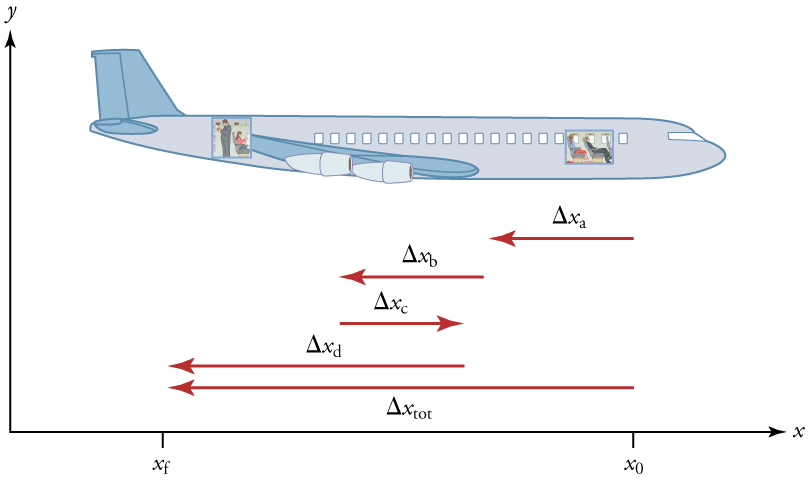
\includegraphics{images/Figure_02_02_01.jpg}
\caption{A more detailed record of an airplane passenger heading toward the
back of the plane, showing smaller segments of his
trip.}\label{import-auto-id1782958}
}
\end{figure}

The smaller the time intervals considered in a motion, the more detailed
the information. When we carry this process to its logical conclusion,
we are left with an infinitesimally small interval. Over such an
interval, the average velocity becomes the \emph{instantaneous velocity}
\emph{}or the \emph{velocity at a specific instant}.
A car's speedometer, for example, shows the magnitude (but not the
direction) of the instantaneous velocity of the car. (Police give
tickets based on instantaneous velocity, but when calculating how long
it will take to get from one place to another on a road trip, you need
to use average velocity.) \protect\hypertarget{import-auto-id2579029}{}{Instantaneous
velocity} \(v{}\) is the average
velocity at a specific instant in time (or over an infinitesimally small
time interval).

Mathematically, finding instantaneous velocity, \(v{}\), at a precise
instant \(t{}\) can involve taking a limit, a calculus operation beyond
the scope of this text. However, under many circumstances, we can find
precise values for instantaneous velocity without calculus.

\hypertarget{fs-id3597726}{}
\hypertarget{speed}{%
\subsection{Speed}\label{speed}}

In everyday language, most people use the terms ``speed'' and ``velocity''
interchangeably. In physics, however, they do not have the same meaning
and they are distinct concepts. One major difference is that speed has
no direction. Thus \emph{speed is a scalar}. Just as we need to distinguish
between instantaneous velocity and average velocity, we also need to
distinguish between instantaneous speed and average speed.

\protect\hypertarget{import-auto-id2004213}{}{Instantaneous speed} is the
magnitude of instantaneous velocity. For example, suppose the airplane
passenger at one instant had an instantaneous velocity of −3.0 m/s (the
minus meaning toward the rear of the plane). At that same time his
instantaneous speed was 3.0 m/s. Or suppose that at one time during a
shopping trip your instantaneous velocity is 40 km/h due north. Your
instantaneous speed at that instant would be 40 km/h---the same
magnitude but without a direction. Average speed, however, is very
different from average velocity. \protect\hypertarget{import-auto-id2004216}{}{Average speed} is the distance traveled divided by elapsed time.

We have noted that distance traveled can be greater than displacement.
So average speed can be greater than average velocity, which is
displacement divided by time. For example, if you drive to a store and
return home in half an hour, and your car's odometer shows the total
distance traveled was 6 km, then your average speed was 12 km/h. Your
average velocity, however, was zero, because your displacement for the
round trip is zero. (Displacement is change in position and, thus, is
zero for a round trip.) Thus average speed is \emph{not} simply the magnitude
of average velocity.

\begin{figure}
\hypertarget{import-auto-id2593426}{%
\centering
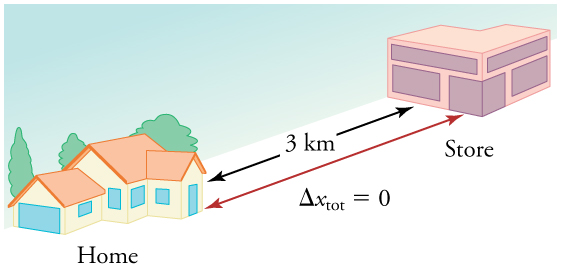
\includegraphics{images/Figure_02_02_02.jpg}
\caption{During a 30-minute round trip to the store, the total distance
traveled is 6 km. The average speed is 12 km/h. The displacement for the
round trip is zero, since there was no net change in position. Thus the
average velocity is
zero.}\label{import-auto-id2593426}
}
\end{figure}

Another way of visualizing the motion of an object is to use a graph. A
plot of position or of velocity as a function of time can be very
useful. For example, for this trip to the store, the position, velocity,
and speed-vs.-time graphs are displayed in
\protect\hyperlink{import-auto-id1806646}{link}. (Note that these
graphs depict a very simplified \protect\hypertarget{import-auto-id1510828}{}{model} of the trip. We are assuming that speed is constant
during the trip, which is unrealistic given that we'll probably stop at
the store. But for simplicity's sake, we will model it with no stops or
changes in speed. We are also assuming that the route between the store
and the house is a perfectly straight line.)

\begin{figure}
\hypertarget{import-auto-id1806646}{%
\centering
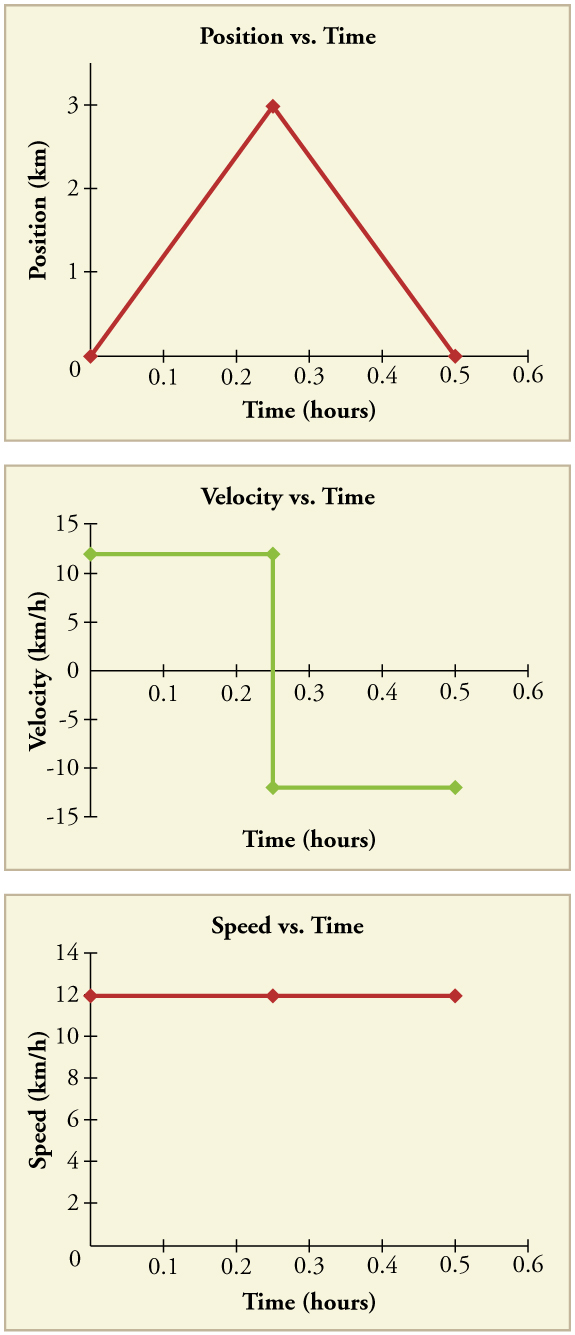
\includegraphics{images/Figure_02_02_03.jpg}
\caption{Position vs.~time, velocity vs.~time, and speed vs.~time on a trip.
Note that the velocity for the return trip is
negative.}\label{import-auto-id1806646}
}
\end{figure}

\hypertarget{fs-id4030893}{}
\begin{note}

Making Connections: Take-Home Investigation---Getting a Sense of Speed

If you have spent much time driving, you probably have a good sense of
speeds between about 10 and 70 miles per hour. But what are these in
meters per second? What do we mean when we say that something is moving
at 10 m/s? To get a better sense of what these values really mean, do
some observations and calculations on your own:

\begin{itemize}
\tightlist
\item
  \protect\hypertarget{import-auto-id4058974}{}{calculate typical car speeds in meters per
  second}
\item
  \protect\hypertarget{import-auto-id4058977}{}{estimate jogging and walking speed by timing yourself; convert the
  measurements into both m/s and mi/h}
\item
  \protect\hypertarget{import-auto-id4070923}{}{determine the speed of an ant, snail, or falling
  leaf}
\end{itemize}

\end{note}

\hypertarget{fs-id4173641}{}
Check Your Understanding

\leavevmode\hypertarget{fs-id1744684}{}%
A commuter train travels from Baltimore to Washington, DC, and back in 1
hour and 45 minutes. The distance between the two stations is
approximately 40 miles. What is (a) the average velocity of the train,
and (b) the average speed of the train in m/s?

\leavevmode\hypertarget{fs-id1384034}{}%
\(a\) The average velocity of the train is zero because
\({x_{f} = x_{0}}{}\); the train ends up at the same place it starts.

\(b\) The average speed of the train is calculated below. Note that the
train travels 40 miles one way and 40 miles back, for a total distance
of 80 miles.

\leavevmode\hypertarget{import-auto-id4070756}{}%
\[{\frac{\text{distance}}{\text{time}} = \frac{\text{80\ miles}}{\text{105\ minutes}}}{}\]

\leavevmode\hypertarget{import-auto-id1750086}{}%
\[{{{\frac{\text{80\ miles}}{\text{105\ minutes}} \times \frac{\text{5280\ feet}}{\text{1\ mile}}} \times \frac{\text{1\ meter}}{3\text{.}\text{28\ feet}}} \times \frac{\text{1\ minute}}{\text{60\ seconds}}} = \text{20\ m/s}\]

\hypertarget{fs-id1345097-summary}{}
\hypertarget{section-summary-2}{%
\subsection{Section Summary}\label{section-summary-2}}

\begin{itemize}
\item
  \protect\hypertarget{import-auto-id4070541}{}{Time is measured in terms of change, and its SI unit is the second
  (s). Elapsed time for an event is}
  ::: \{\#import-auto-id4146177 data-type=``equation''\}
  \[{\Delta t = {t_{f} - t_{0}},}{}\]

  :::

  where \(t_{f}{}\) is the final time and
  \emph{}\(t_{0}{}\) is the initial time. The
  initial time is often taken to be zero, as if measured with a
  stopwatch; the elapsed time is then just \(t{}\).
\item
  \protect\hypertarget{import-auto-id1770783}{}{Average velocity \(\overset{-}{v}{}\) is defined as displacement
  divided by the travel time. In symbols, average velocity
  is}
  ::: \{\#import-auto-id4086565 data-type=``equation''\}
  \[{{{\overset{-}{v} = \frac{\Delta x}{\Delta t}} = \frac{x_{\text{f}} - x_{0}}{t_{\text{f}} - t_{0}}}\text{.}}{}\]

  :::
\item
  \protect\hypertarget{import-auto-id1795857}{}{The SI unit for velocity is m/s.}
\item
  \protect\hypertarget{import-auto-id1795847}{}{Velocity is a vector and thus has a
  direction.}
\item
  \protect\hypertarget{import-auto-id4097170}{}{Instantaneous velocity \(v{}\) is the velocity at a specific instant
  or the average velocity for an infinitesimal
  interval.}
\item
  \protect\hypertarget{import-auto-id4097153}{}{Instantaneous speed is the magnitude of the instantaneous
  velocity.}
\item
  \protect\hypertarget{import-auto-id4097155}{}{Instantaneous speed is a scalar quantity, as it has no direction
  specified.}
\item
  \protect\hypertarget{import-auto-id4097159}{}{Average speed is the total distance traveled divided by the elapsed
  time. (Average speed is \emph{not} the magnitude of the average
  velocity.) Speed is a scalar quantity; it has no direction
  associated with it.}
\end{itemize}

\hypertarget{fs-id3505230}{}
\begin{conceptual-questions}

\hypertarget{conceptual-questions-2}{%
\subsection{Conceptual Questions}\label{conceptual-questions-2}}

\hypertarget{fs-id4081795}{}
\leavevmode\hypertarget{fs-id4057370}{}%
Give an example (but not one from the text) of a device used to measure
time and identify what change in that device indicates a change in time.

\hypertarget{fs-id4059976}{}
\leavevmode\hypertarget{fs-id4059193}{}%
There is a distinction between average speed and the magnitude of
average velocity. Give an example that illustrates the difference
between these two quantities.

\hypertarget{fs-id3539434}{}
\leavevmode\hypertarget{fs-id1765012}{}%
Does a car's odometer measure position or displacement? Does its
speedometer measure speed or velocity?

\hypertarget{fs-id4033346}{}
\leavevmode\hypertarget{fs-id1181844}{}%
If you divide the total distance traveled on a car trip (as determined
by the odometer) by the time for the trip, are you calculating the
average speed or the magnitude of the average velocity? Under what
circumstances are these two quantities the same?

\hypertarget{fs-id1798382}{}
\leavevmode\hypertarget{fs-id3586650}{}%
How are instantaneous velocity and instantaneous speed related to one
another? How do they differ?

\end{conceptual-questions}

\hypertarget{fs-id1644454}{}
\begin{problems-exercises}

\hypertarget{problems-exercises-1}{%
\subsection{Problems \& Exercises}\label{problems-exercises-1}}

\hypertarget{fs-id4131776}{}
\leavevmode\hypertarget{fs-id1489911}{}%
\(a\) Calculate Earth's average speed relative to the Sun. (b) What is
its average velocity over a period of one year?

\leavevmode\hypertarget{fs-id3602083}{}%
\(a\) \({3\text{.}{\text{0} \times \text{10}^{4}\ }\text{m/s}}{}\)

\(b\) 0 m/s

\hypertarget{fs-id3514248}{}
\leavevmode\hypertarget{fs-id1773543}{}%
A helicopter blade spins at exactly 100 revolutions per minute. Its tip
is 5.00 m from the center of rotation. (a) Calculate the average speed
of the blade tip in the helicopter's frame of reference. (b) What is
its average velocity over one revolution?

\hypertarget{fs-id1438634}{}
\leavevmode\hypertarget{fs-id1738040}{}%
The North American and European continents are moving apart at a rate of
about 3 cm/y. At this rate how long will it take them to drift 500 km
farther apart than they are at present?

\leavevmode\hypertarget{fs-id2587370}{}%
\({{2 \times \text{10}^{7}}\ \text{years}}{}\)

\hypertarget{fs-id2572316}{}
\leavevmode\hypertarget{fs-id1275687}{}%
Land west of the San Andreas fault in southern California is moving at
an average velocity of about 6 cm/y northwest relative to land east of
the fault. Los Angeles is west of the fault and may thus someday be at
the same latitude as San Francisco, which is east of the fault. How far
in the future will this occur if the displacement to be made is 590 km
northwest, assuming the motion remains constant?

\hypertarget{fs-id1403452}{}
\leavevmode\hypertarget{fs-id1357553}{}%
On May 26, 1934, a streamlined, stainless steel diesel train called the
Zephyr set the world's nonstop long-distance speed record for trains.
Its run from Denver to Chicago took 13 hours, 4 minutes, 58 seconds, and
was witnessed by more than a million people along the route. The total
distance traveled was 1633.8 km. What was its average speed in km/h and
m/s?

\leavevmode\hypertarget{fs-id4081588}{}%
\(\text{34}\text{.}\text{689\ m/s} = \text{124}\text{.}\text{88\ km/h}\)

\hypertarget{fs-id951583}{}
\leavevmode\hypertarget{fs-id1535186}{}%
Tidal friction is slowing the rotation of the Earth. As a result, the
orbit of the Moon is increasing in radius at a rate of approximately 4
cm/year. Assuming this to be a constant rate, how many years will pass
before the radius of the Moon's orbit increases by
\({3\text{.}{\text{84} \times \text{10}^{6}}\ m}{}\) (1\%)?

\hypertarget{fs-id1271475}{}
\leavevmode\hypertarget{fs-id1544659}{}%
A student drove to the university from her home and noted that the
odometer reading of her car increased by 12.0 km. The trip took 18.0
min. (a) What was her average speed? (b) If the straight-line distance
from her home to the university is 10.3 km in a direction
\({\text{25}\text{.}0º}{}\) south of east, what was her average velocity?
(c) If she returned home by the same path 7 h 30 min after she left,
what were her average speed and velocity for the entire trip?

\leavevmode\hypertarget{fs-id1780671}{}%
\(a\) \({\text{40}\text{.}\text{0\ km/h}}{}\)

\(b\) 34.3 km/h, \({\text{25º}\ \text{S\ of\ E}\text{.}}{}\)

\(c\)
\({{\text{average\ speed} = \text{3.20\ km/h,}\ \overset{-}{v}} = 0.}{}\)

\hypertarget{fs-id1644060}{}
\leavevmode\hypertarget{fs-id1742458}{}%
The speed of propagation of the action potential (an electrical signal)
in a nerve cell depends (inversely) on the diameter of the axon (nerve
fiber). If the nerve cell connecting the spinal cord to your feet is 1.1
m long, and the nerve impulse speed is 18 m/s, how long does it take for
the nerve signal to travel this distance?

\hypertarget{fs-id1638875}{}
\leavevmode\hypertarget{fs-id2015498}{}%
Conversations with astronauts on the lunar surface were characterized by
a kind of echo in which the earthbound person's voice was so loud in
the astronaut's space helmet that it was picked up by the astronaut's
microphone and transmitted back to Earth. It is reasonable to assume
that the echo time equals the time necessary for the radio wave to
travel from the Earth to the Moon and back (that is, neglecting any time
delays in the electronic equipment). Calculate the distance from Earth
to the Moon given that the echo time was 2.56 s and that radio waves
travel at the speed of light
\((3\text{.}{\text{00} \times \text{10}^{8}\ }\text{m/s})\).

\leavevmode\hypertarget{fs-id1659453}{}%
384,000 km

\hypertarget{fs-id2577314}{}
\leavevmode\hypertarget{fs-id4044402}{}%
A football quarterback runs 15.0 m straight down the playing field in
2.50 s. He is then hit and pushed 3.00 m straight backward in 1.75 s. He
breaks the tackle and runs straight forward another 21.0 m in 5.20 s.
Calculate his average velocity (a) for each of the three intervals and
(b) for the entire motion.

\hypertarget{fs-id4047255}{}
\leavevmode\hypertarget{fs-id4047256}{}%
The planetary model of the atom pictures electrons orbiting the atomic
nucleus much as planets orbit the Sun. In this model you can view
hydrogen, the simplest atom, as having a single electron in a circular
orbit \(1\text{.}\text{06} \times \text{10}^{- \text{10}}\ \text{m}\) in
diameter. (a) If the average speed of the electron in this orbit is
known to be \(2\text{.}{\text{20} \times \text{10}^{6}}\ \text{m/s}\),
calculate the number of revolutions per second it makes about the
nucleus. (b) What is the electron's average velocity?

\leavevmode\hypertarget{fs-id2580487}{}%
\(a\)
\({6\text{.}{\text{61} \times \text{10}^{\text{15}}}\ \text{rev/s}}{}\)

\(b\) 0 m/s

\end{problems-exercises}

\hypertarget{fs-id1283687}{}
\begin{ap-test-prep}

\hypertarget{test-prep-for-ap-courses-2}{%
\subsection{Test Prep for AP Courses}\label{test-prep-for-ap-courses-2}}

\hypertarget{fs-id2172989}{}
\leavevmode\hypertarget{fs-id2066649}{}%
A group of students has two carts, \emph{A} and \emph{B}, with wheels that turn
with negligible friction. The two carts travel along a straight
horizontal track and eventually collide. Before the collision, cart \emph{A}
travels to the right and cart \emph{B} is initially at rest. After the
collision, the carts stick together.

\begin{enumerate}
\def\labelenumi{\alph{enumi}.}
\tightlist
\item
  Describe an experimental procedure to determine the velocities of
  the carts before and after the collision, including all the
  additional equipment you would need. You may include a labeled
  diagram of your setup to help in your description. Indicate what
  measurements you would take and how you would take them. Include
  enough detail so that another student could carry out your
  procedure.
\item
  There will be sources of error in the measurements taken in the
  experiment both before and after the collision. Which velocity will
  be more greatly affected by this error: the velocity prior to the
  collision or the velocity after the collision? Or will both sets of
  data be affected equally? Justify your answer.
\end{enumerate}

\hypertarget{fs-id1336990}{}
\begin{enumerate}
\def\labelenumi{\alph{enumi}.}
\tightlist
\item
  Use tape to mark off two distances on the track --- one for cart \emph{A}
  before the collision and one for the combined carts after the
  collision. Push cart \emph{A} to give it an initial speed. Use a
  stopwatch to measure the time it takes for the cart(s) to cross the
  marked distances. The speeds are the distances divided by the times.
\item
  If the measurement errors are of the same magnitude, they will have
  a greater effect after the collision. The speed of the combined
  carts will be less than the initial speed of cart \emph{A}. As a result,
  these errors will be a greater percentage of the actual velocity
  value after the collision occurs. (Note: Other arguments could
  properly be made for 'more error before the collision' and error
  that 'equally affects both sets of measurement.')
\end{enumerate}

\end{ap-test-prep}

\hypertarget{glossary-2}{%
\subsection{Glossary}\label{glossary-2}}

\begin{description}
\tightlist
\item[average speed]
distance traveled divided by time during which motion occurs
\end{description}

\begin{description}
\tightlist
\item[average velocity]
displacement divided by time over which displacement occurs
\end{description}

\begin{description}
\tightlist
\item[instantaneous velocity]
velocity at a specific instant, or the average velocity over an
infinitesimal time interval
\end{description}

\begin{description}
\tightlist
\item[instantaneous speed]
magnitude of the instantaneous velocity
\end{description}

\begin{description}
\tightlist
\item[time]
change, or the interval over which change occurs
\end{description}

\begin{description}
\tightlist
\item[model]
simplified description that contains only those elements necessary
to describe the physics of a physical situation
\end{description}

\begin{description}
\tightlist
\item[elapsed time]
the difference between the ending time and beginning time
\end{description}

\hypertarget{acceleration}{%
\section{Acceleration}\label{acceleration}}

\begin{figure}
\hypertarget{import-auto-id3514068}{%
\centering
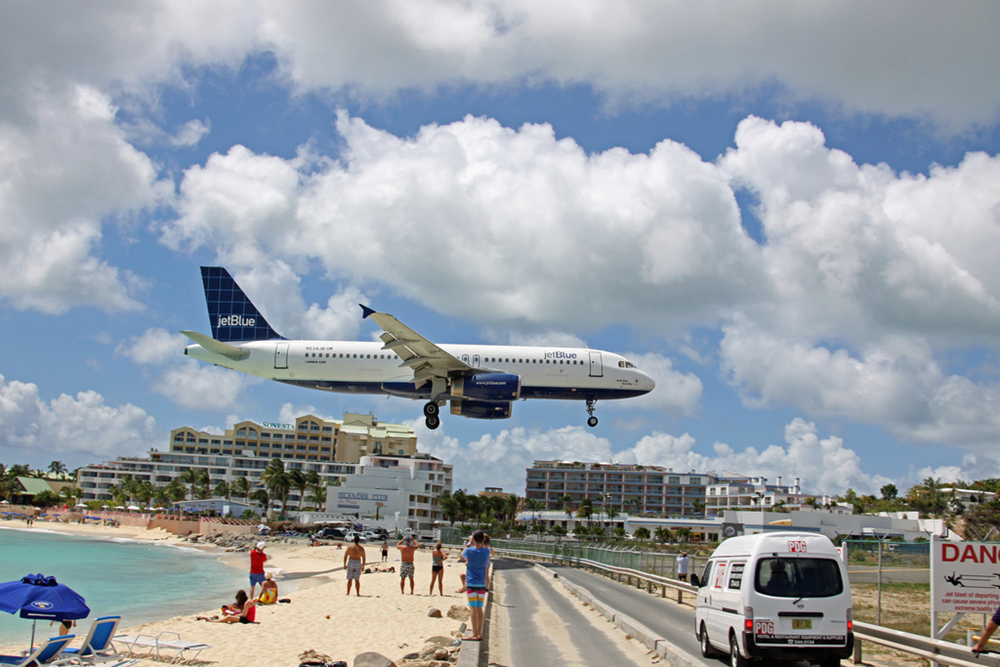
\includegraphics{images/Figure_02_04_00.jpg}
\caption{A plane decelerates, or slows down, as it comes in for landing in St.
Maarten. Its acceleration is opposite in direction to its velocity.
(credit: Steve Conry,
Flickr)}\label{import-auto-id3514068}
}
\end{figure}

\hypertarget{fs-id1271912}{}
\begin{learning-objectives}

\hypertarget{learning-objectives-2}{%
\subsection{Learning Objectives}\label{learning-objectives-2}}

By the end of this section, you will be able to:

\begin{itemize}
\tightlist
\item
  Define and distinguish between instantaneous acceleration and
  average acceleration.
\item
  Calculate acceleration given initial time, initial velocity, final
  time, and final velocity.
\end{itemize}

The information presented in this section supports the following AP®
learning objectives and science practices:

\begin{itemize}
\tightlist
\item
  \textbf{3.A.1.1} The student is able to express the motion of an object
  using narrative, mathematical, and graphical representations.
  \textbf{(S.P. 1.5, 2.1, 2.2)}
\item
  \textbf{3.A.1.3} The student is able to analyze experimental data
  describing the motion of an object and is able to express the
  results of the analysis using narrative, mathematical, and graphical
  representations. \textbf{(S.P. 5.1)}
\end{itemize}

\end{learning-objectives}

In everyday conversation, to accelerate means to speed up. The
accelerator in a car can in fact cause it to speed up. The greater the
\protect\hypertarget{import-auto-id1298945}{}{acceleration}, the greater the
change in velocity over a given time. The formal definition of
acceleration is consistent with these notions, but more inclusive.

\hypertarget{fs-id4053362}{}
\begin{note}

Average Acceleration

\protect\hypertarget{import-auto-id2580108}{}{Average Acceleration} is \emph{the
rate at which velocity changes},

\leavevmode\hypertarget{import-auto-id4040806}{}%
\[{{{\overset{-}{a} = \frac{\Delta v}{\Delta t}} = \frac{v_{f}{- v_{0}}}{t_{f} - t_{0}}},}{}\]

where \emph{\(\overset{-}{a}{}\)} is average acceleration, \emph{\(v{}\)} is velocity,
and \emph{\(t{}\)} is time. (The bar over the \(a{}\) means \emph{average}
acceleration.)

\end{note}

Because acceleration is velocity in m/s divided by time in s, the SI
units for acceleration are \(\text{m/s}^{2}{}\), meters per second squared
or meters per second per second, which literally means by how many
meters per second the velocity changes every second.

Recall that velocity is a vector---it has both magnitude and direction.
This means that a change in velocity can be a change in magnitude (or
speed), but it can also be a change in \emph{direction}. For example, if a
car turns a corner at constant speed, it is accelerating because its
direction is changing. The quicker you turn, the greater the
acceleration. So there is an acceleration when velocity changes either
in magnitude (an increase or decrease in speed) or in direction, or
both.

\hypertarget{fs-id3524141}{}
\begin{note}

Acceleration as a Vector

Acceleration is a vector in the same direction as the \emph{change} in
velocity, \({\Delta v}{}\). Since velocity is a vector, it can change
either in magnitude or in direction. Acceleration is therefore a change
in either speed or direction, or both.

\end{note}

Keep in mind that although acceleration is in the direction of the
\emph{change} in velocity, it is not always in the direction of \emph{motion}.
When an object's acceleration is in the same direction of its motion,
the object will speed up. However, when an object's acceleration is
opposite to the direction of its motion, the object will slow down.
Speeding up and slowing down should not be confused with a positive and
negative acceleration. The next two examples should help to make this
distinction clear.

\begin{figure}
\hypertarget{import-auto-id1515319}{%
\centering
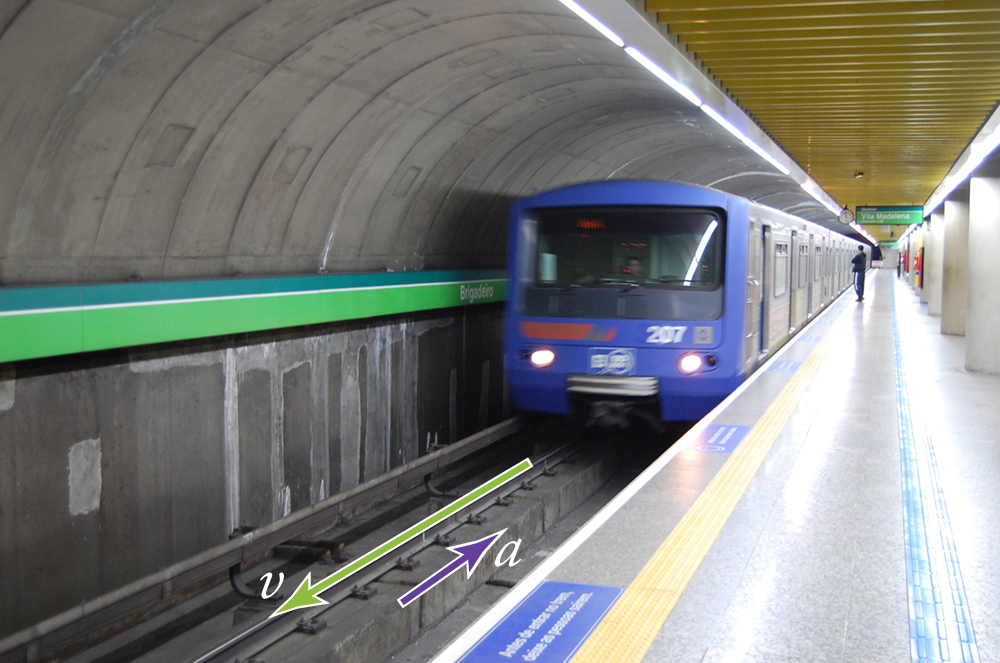
\includegraphics{images/Figure_02_04_00a.jpg}
\caption{A subway train in Sao Paulo, Brazil, decelerates as it comes into a
station. It is accelerating in a direction opposite to its direction of
motion. (credit: Yusuke Kawasaki,
Flickr)}\label{import-auto-id1515319}
}
\end{figure}

\hypertarget{fs-id1389422}{}
\begin{note}

Making Connections: Car Motion

\begin{figure}
\hypertarget{import-auto-id3579626}{%
\centering
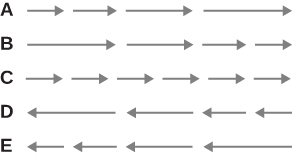
\includegraphics{images/Figure_Ch2_M4_01.jpg}
\caption{Above are arrows representing the motion of five cars (A--E). In all
five cases, the positive direction should be considered to the right of
the page.}\label{import-auto-id3579626}
}
\end{figure}

Consider the acceleration and velocity of each car in terms of its
direction of travel.

\begin{figure}
\hypertarget{fs-id2218162}{%
\centering
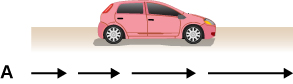
\includegraphics{images/Figure_Ch2_M4_02.jpg}
\caption{Car A is speeding up.}\label{fs-id2218162}
}
\end{figure}

Because the positive direction is considered to the right of the paper,
Car A is moving with a positive velocity. Because it is speeding up
while moving with a positive velocity, its acceleration is also
considered positive.

\begin{figure}
\hypertarget{fs-id3242689}{%
\centering
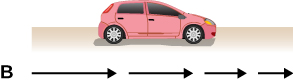
\includegraphics{images/Figure_Ch2_M4_03.jpg}
\caption{Car B is slowing down.}\label{fs-id3242689}
}
\end{figure}

Because the positive direction is considered to the right of the paper,
Car B is also moving with a positive velocity. However, because it is
slowing down while moving with a positive velocity, its acceleration is
considered negative. (This can be viewed in a mathematical manner as
well. If the car was originally moving with a velocity of +25 m/s, it is
finishing with a speed less than that, like +5 m/s. Because the change
in velocity is negative, the acceleration will be as well.)

\begin{figure}
\hypertarget{fs-id2186010}{%
\centering
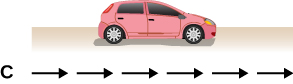
\includegraphics{images/Figure_Ch2_M4_04.jpg}
\caption{Car C has a constant
speed.}\label{fs-id2186010}
}
\end{figure}

Because the positive direction is considered to the right of the paper,
Car C is moving with a positive velocity. Because all arrows are of the
same length, this car is not changing its speed. As a result, its change
in velocity is zero, and its acceleration must be zero as well.

\begin{figure}
\hypertarget{fs-id2672786}{%
\centering
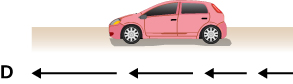
\includegraphics{images/Figure_Ch2_M4_05.jpg}
\caption{Car D is speeding up in the opposite direction of Cars A, B,
C.}\label{fs-id2672786}
}
\end{figure}

Because the car is moving opposite to the positive direction, Car D is
moving with a negative velocity. Because it is speeding up while moving
in a negative direction, its acceleration is negative as well.

\begin{figure}
\hypertarget{fs-id1956758}{%
\centering
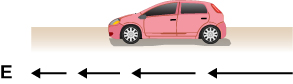
\includegraphics{images/Figure_Ch2_M4_06.jpg}
\caption{Car E is slowing down in the same direction as Car D and opposite of
Cars A, B, C.}\label{fs-id1956758}
}
\end{figure}

Because it is moving opposite to the positive direction, Car E is moving
with a negative velocity as well. However, because it is slowing down
while moving in a negative direction, its acceleration is actually
positive. As in example B, this may be more easily understood in a
mathematical sense. The car is originally moving with a large negative
velocity (−25 m/s) but slows to a final velocity that is less negative
(−5 m/s). This change in velocity, from −25 m/s to −5 m/s, is actually a
positive change (
\(v_{f} - v_{i} = \operatorname{} - 5\text{~m/s~} - - 25\text{~m/s}\) of
20 m/s. Because the change in velocity is positive, the acceleration
must also be positive.

\end{note}

\hypertarget{fs-id1050890}{}
\begin{note}

Making Connection - Illustrative Example

The three graphs below are labeled A, B, and C. Each one represents the
position of a moving object plotted against time.

\begin{figure}
\hypertarget{fs-id2024196}{%
\centering
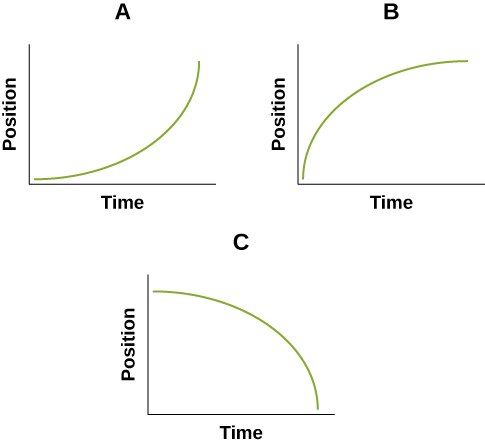
\includegraphics{images/CNX_APPhysics_02_M4_graphoverv.jpg}
\caption{Three position and time graphs: A, B, and
C.}\label{fs-id2024196}
}
\end{figure}

As we did in the previous example, let's consider the acceleration and
velocity of each object in terms of its direction of travel.

\begin{figure}
\hypertarget{fs-id2217910}{%
\centering
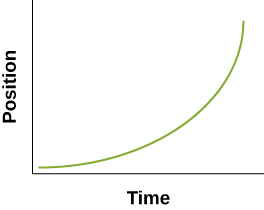
\includegraphics{images/Figure_Ch2_M4_08.jpg}
\caption{Graph A of Position (y axis) vs.~Time (x
axis).}\label{fs-id2217910}
}
\end{figure}

Object A is continually increasing its position in the positive
direction. As a result, its velocity is considered positive.

\begin{figure}
\hypertarget{fs-id1850704}{%
\centering
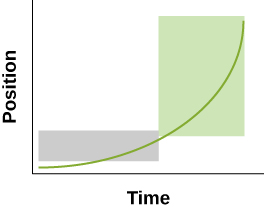
\includegraphics{images/Figure_Ch2_M4_09.jpg}
\caption{Breakdown of Graph A into two separate
sections.}\label{fs-id1850704}
}
\end{figure}

During the first portion of time (shaded grey) the position of the
object does not change much, resulting in a small positive velocity.
During a later portion of time (shaded green) the position of the object
changes more, resulting in a larger positive velocity. Because this
positive velocity is increasing over time, the acceleration of the
object is considered positive.

\begin{figure}
\hypertarget{fs-id3207940}{%
\centering
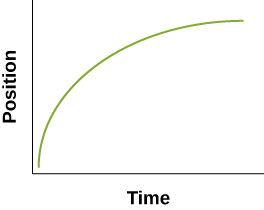
\includegraphics{images/Figure_Ch2_M4_10.jpg}
\caption{Graph B of Position (y axis) vs.~Time (x
axis).}\label{fs-id3207940}
}
\end{figure}

As in case A, Object B is continually increasing its position in the
positive direction. As a result, its velocity is considered positive.

\begin{figure}
\hypertarget{fs-id3195153}{%
\centering
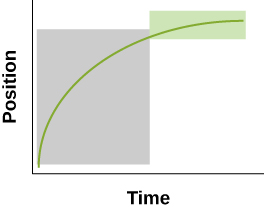
\includegraphics{images/Figure_Ch2_M4_11.jpg}
\caption{Breakdown of Graph B into two separate
sections.}\label{fs-id3195153}
}
\end{figure}

During the first portion of time (shaded grey) the position of the
object changes a large amount, resulting in a large positive velocity.
During a later portion of time (shaded green) the position of the object
does not change as much, resulting in a smaller positive velocity.
Because this positive velocity is decreasing over time, the acceleration
of the object is considered negative.

\begin{figure}
\hypertarget{fs-id2059002}{%
\centering
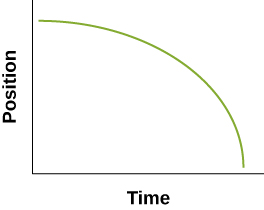
\includegraphics{images/Figure_Ch2_M4_12.jpg}
\caption{Graph C of Position (y axis) vs.~Time (x
axis).}\label{fs-id2059002}
}
\end{figure}

Object C is continually decreasing its position in the positive
direction. As a result, its velocity is considered negative.

\begin{figure}
\hypertarget{fs-id2387653}{%
\centering
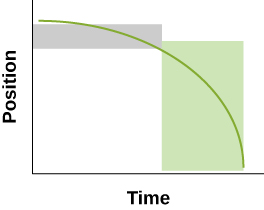
\includegraphics{images/Figure_Ch2_M4_13.jpg}
\caption{Breakdown of Graph C into two separate
sections.}\label{fs-id2387653}
}
\end{figure}

During the first portion of time (shaded grey) the position of the
object does not change a large amount, resulting in a small negative
velocity. During a later portion of time (shaded green) the position of
the object changes a much larger amount, resulting in a larger negative
velocity. Because the velocity of the object is becoming more negative
during the time period, the change in velocity is negative. As a result,
the object experiences a negative acceleration.

\end{note}

\hypertarget{fs-id2013623}{}
Calculating Acceleration: A Racehorse Leaves the Gate

A racehorse coming out of the gate accelerates from rest to a velocity
of 15.0 m/s due west in 1.80 s. What is its average acceleration?

\begin{figure}
\hypertarget{import-auto-id1806246}{%
\centering
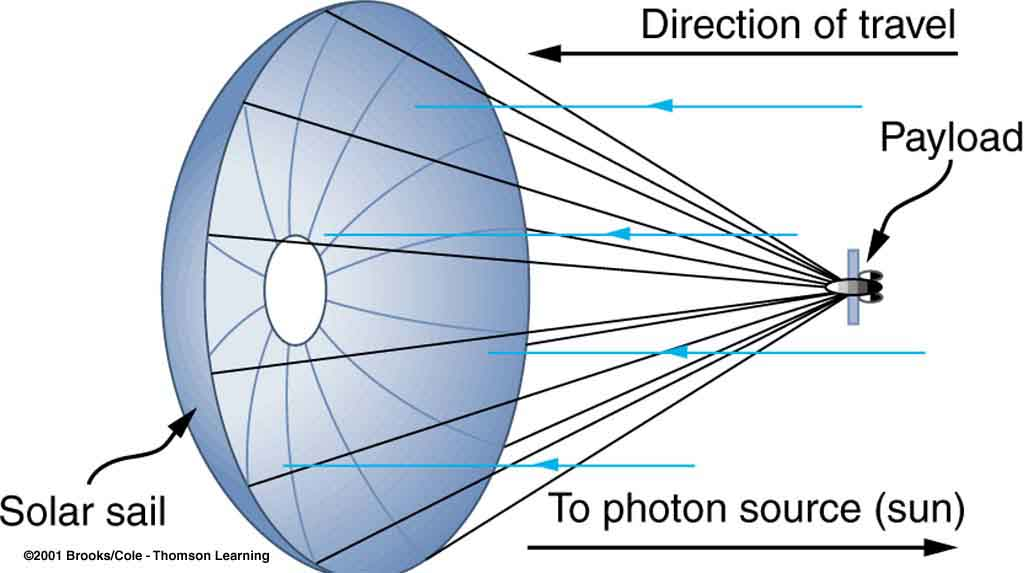
\includegraphics{images/graphics4.jpg}
\caption{(credit: Jon Sullivan, PD
Photo.org)}\label{import-auto-id1806246}
}
\end{figure}

\begin{tinysection}

{Strategy}

\end{tinysection}

First we draw a sketch and assign a coordinate system to the problem.
This is a simple problem, but it always helps to visualize it. Notice
that we assign east as positive and west as negative. Thus, in this
case, we have negative velocity.

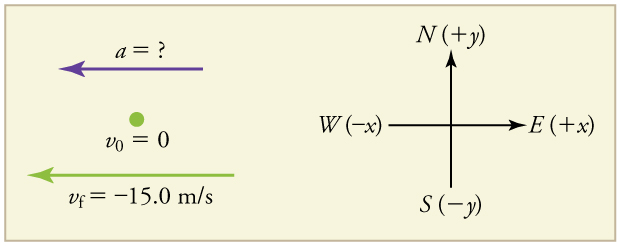
\includegraphics{images/Figure_02_03_01a.jpg}

We can solve this problem by identifying \({\Delta v}{}\) and
\({\Delta t}{}\) from the given information and then calculating the
average acceleration directly from the equation
\({{\overset{-}{a} = \frac{\Delta v}{\Delta t}} = \frac{v_{f}{- v_{0}}}{t_{f} - t_{0}}}{}\).

\begin{tinysection}

{Solution}

\end{tinysection}

1. Identify the knowns. \({v_{0} = 0}{}\),
\({v_{f} = {- \text{15}}}\text{.0\ m/s}\) (the minus sign indicates
direction toward the west), \({{\Delta t = 1}\text{.80\ s}}{}\).

2. Find the change in velocity. Since the horse is going from zero to
\({- \text{15.0\ m/s}}{}\), its change in velocity equals its final
velocity: \({{{\Delta v = v_{f}} = {- \text{15}}}\text{.0\ m/s}}{}\).

3. Plug in the known values (\({\Delta v}{}\) and \(\Delta t\)) and solve
for the unknown \(\overset{-}{a}{}\).

\leavevmode\hypertarget{import-auto-id2400983}{}%
\[{{{{{\overset{-}{a} = \frac{\Delta v}{\Delta t}} = \,\frac{{- \text{15}}\text{.0\ m/s}}{1\text{.80\ s}}} = {- 8}}\text{.33\ m}\text{/s}^{2}}.}{}\]

\begin{tinysection}

{Discussion}

\end{tinysection}

The minus sign for acceleration indicates that acceleration is toward
the west. An acceleration of \({8\text{.33\ m}\text{/s}^{2}}{}\) due west
means that the horse increases its velocity by 8.33 m/s due west each
second, that is, 8.33 meters per second per second, which we write as
\({8\text{.33\ m}\text{/s}^{2}}{}\). This is truly an average
acceleration, because the ride is not smooth. We shall see later that an
acceleration of this magnitude would require the rider to hang on with a
force nearly equal to his weight.

\hypertarget{fs-id1759915}{}
\hypertarget{instantaneous-acceleration}{%
\subsection{Instantaneous Acceleration}\label{instantaneous-acceleration}}

\protect\hypertarget{import-auto-id2303194}{}{Instantaneous acceleration}
\(a{}\), or the \emph{acceleration at a specific instant in time}, is obtained
by the same process as discussed for instantaneous velocity in \href{/m54771}{Time,
Velocity, and Speed}---that is, by considering an
infinitesimally small interval of time. How do we find instantaneous
acceleration using only algebra? The answer is that we choose an average
acceleration that is representative of the motion.
\protect\hyperlink{import-auto-id2590846}{link} shows graphs of
instantaneous acceleration versus time for two very different motions.
In \protect\hyperlink{import-auto-id2590846}{link}(a), the
acceleration varies slightly and the average over the entire interval is
nearly the same as the instantaneous acceleration at any time. In this
case, we should treat this motion as if it had a constant acceleration
equal to the average (in this case about
\({1\text{.}8\ m\text{/s}^{2}}{}\)). In
\protect\hyperlink{import-auto-id2590846}{link}(b), the
acceleration varies drastically over time. In such situations it is best
to consider smaller time intervals and choose an average acceleration
for each. For example, we could consider motion over the time intervals
from 0 to 1.0 s and from 1.0 to 3.0 s as separate motions with
accelerations of \({+ 3}\text{.}0\ m\text{/s}^{2}\) and
\(\text{–2}\text{.}0\ m\text{/s}^{2}\), respectively.

\begin{figure}
\hypertarget{import-auto-id2590846}{%
\centering
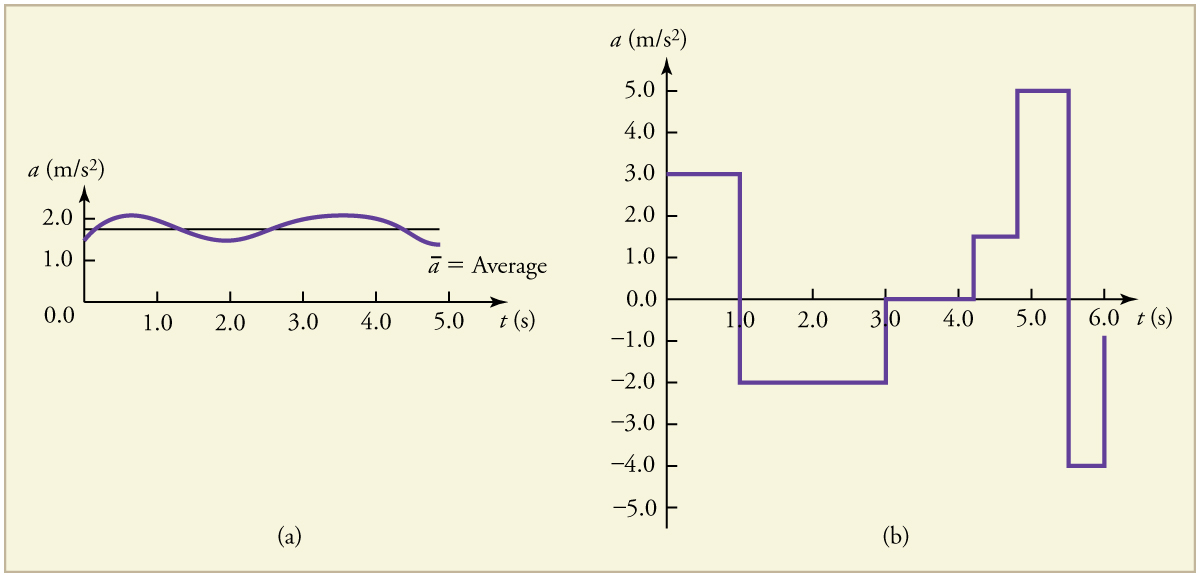
\includegraphics{images/Figure_02_03_02.jpg}
\caption{Graphs of instantaneous acceleration versus time for two different
one-dimensional motions. (a) Here acceleration varies only slightly and
is always in the same direction, since it is positive. The average over
the interval is nearly the same as the acceleration at any given time.
(b) Here the acceleration varies greatly, perhaps representing a package
on a post office conveyor belt that is accelerated forward and backward
as it bumps along. It is necessary to consider small time intervals
(such as from 0 to 1.0 s) with constant or nearly constant acceleration
in such a
situation.}\label{import-auto-id2590846}
}
\end{figure}

The next several examples consider the motion of the subway train shown
in \protect\hyperlink{import-auto-id2590556}{link}. In (a) the
shuttle moves to the right, and in (b) it moves to the left. The
examples are designed to further illustrate aspects of motion and to
illustrate some of the reasoning that goes into solving problems.

\begin{figure}
\hypertarget{import-auto-id2590556}{%
\centering
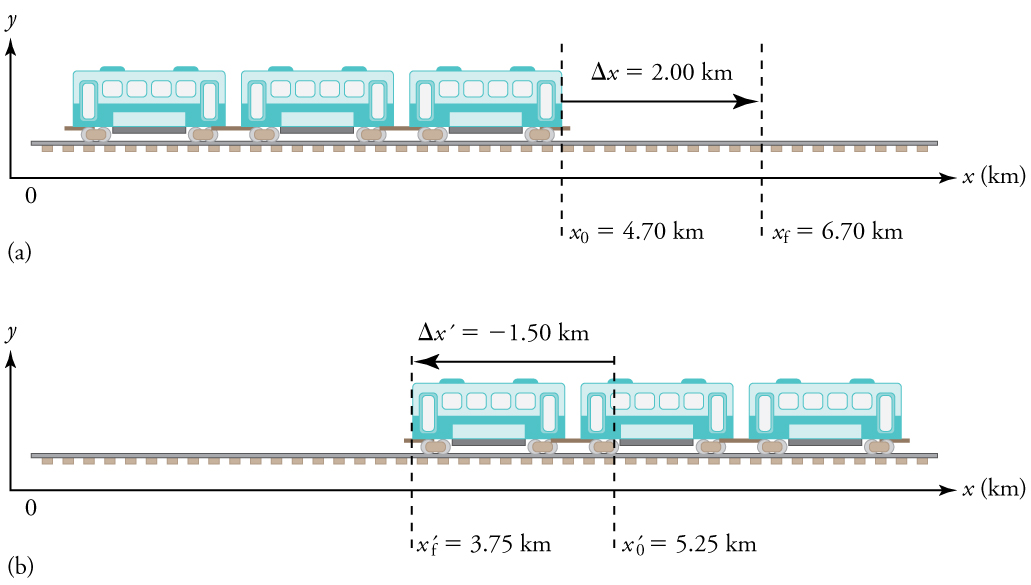
\includegraphics{images/Figure_02_03_03.jpg}
\caption{One-dimensional motion of a subway train considered in
\protect\hyperlink{fs-id1744930}{link},
\protect\hyperlink{fs-id4082275}{link},
\protect\hyperlink{fs-id1372721}{link},
\protect\hyperlink{fs-id3600466}{link},
\protect\hyperlink{fs-id1348757}{link}, and
\protect\hyperlink{fs-id4015260}{link}. Here we have chosen the
\(x{}\)-axis so that + means to the right and \(- {}\) means to the left for
displacements, velocities, and accelerations. (a) The subway train moves
to the right from \(x_{0}{}\) to \(x_{f}\). Its displacement \(\Delta x\) is
+2.0 km. (b) The train moves to the left from \({x\prime}_{0}\) to
\({x\prime}_{f}{}\). Its displacement \({\Delta x\prime}{}\) is
\({{- 1}\text{.5\ km}}{}\). (Note that the prime symbol (′) is used simply
to distinguish between displacement in the two different situations. The
distances of travel and the size of the cars are on different scales to
fit everything into the
diagram.)}\label{import-auto-id2590556}
}
\end{figure}

\hypertarget{fs-id1744930}{}
Calculating Displacement: A Subway Train

What are the magnitude and sign of displacements for the motions of the
subway train shown in parts (a) and (b) of
\protect\hyperlink{import-auto-id2590556}{link}?

\begin{tinysection}

{Strategy}

\end{tinysection}

A drawing with a coordinate system is already provided, so we don't
need to make a sketch, but we should analyze it to make sure we
understand what it is showing. Pay particular attention to the
coordinate system. To find displacement, we use the equation
\({\Delta x = {x_{f} - x_{0}}}{}\). This is straightforward since the
initial and final positions are given.

\begin{tinysection}

{Solution}

\end{tinysection}

1. Identify the knowns. In the figure we see that
\({x_{f} =}\text{6.70\ km}\) and \({x_{0} =}\text{4.70\ km}\) for part (a),
and \({{x\prime}_{f} = 3}\text{.75\ km}\) and
\({{x\prime}_{0} = 5}\text{.25\ km}\) for part (b).

2. Solve for displacement in part (a).

\leavevmode\hypertarget{import-auto-id2400875}{}%
\[{{{\Delta x = {x_{f} - x_{0}}} = 6}\text{.}{\text{70\ km} - 4}\text{.}\text{70\ km}\text{=}\ \text{+}2\text{.}\text{00\ km}}{}\]

3. Solve for displacement in part (b).

\leavevmode\hypertarget{import-auto-id2589758}{}%
\[\Delta x\prime{{= {{x\prime}_{f} - {x\prime}_{0}}} = \text{3.75\ km} - \text{5.25\ km} = - \text{1.50\ km}}\]

\begin{tinysection}

{Discussion}

\end{tinysection}

The direction of the motion in (a) is to the right and therefore its
displacement has a positive sign, whereas motion in (b) is to the left
and thus has a minus sign.

\hypertarget{fs-id4082275}{}
Comparing Distance Traveled with Displacement: A Subway Train

What are the distances traveled for the motions shown in parts (a) and
(b) of the subway train in
\protect\hyperlink{import-auto-id2590556}{link}?

\begin{tinysection}

{Strategy}

\end{tinysection}

To answer this question, think about the definitions of distance and
distance traveled, and how they are related to displacement. Distance
between two positions is defined to be the magnitude of displacement,
which was found in \protect\hyperlink{fs-id1744930}{link}.
Distance traveled is the total length of the path traveled between the
two positions. (See \href{/m54769}{Displacement}.) In the case of the subway
train shown in \protect\hyperlink{import-auto-id2590556}{link},
the distance traveled is the same as the distance between the initial
and final positions of the train.

\begin{tinysection}

{Solution}

\end{tinysection}

1. The displacement for part (a) was +2.00 km. Therefore, the distance
between the initial and final positions was 2.00 km, and the distance
traveled was 2.00 km.

2. The displacement for part (b) was \(\text{−1.5\ km.}\) Therefore, the
distance between the initial and final positions was 1.50 km, and the
distance traveled was 1.50 km.

\begin{tinysection}

{Discussion}

\end{tinysection}

Distance is a scalar. It has magnitude but no sign to indicate
direction.

\hypertarget{fs-id1372721}{}
Calculating Acceleration: A Subway Train Speeding Up

Suppose the train in
\protect\hyperlink{import-auto-id2590556}{link}(a) accelerates
from rest to 30.0 km/h in the first 20.0 s of its motion. What is its
average acceleration during that time interval?

\begin{tinysection}

{Strategy}

\end{tinysection}

It is worth it at this point to make a simple sketch:

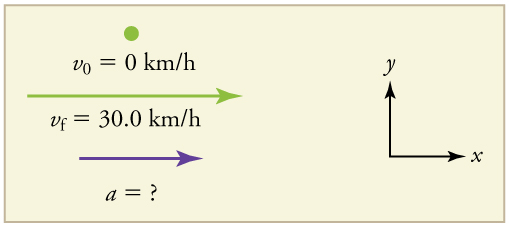
\includegraphics{images/Figure_02_03_03c.jpg}

This problem involves three steps. First we must determine the change in
velocity, then we must determine the change in time, and finally we use
these values to calculate the acceleration.

\begin{tinysection}

{Solution}

\end{tinysection}

1. Identify the knowns. \({v_{0} = 0}{}\) (the trains starts at rest),
\({{v_{f} = \text{30}}\text{.}\text{0\ km/h}}{}\), and
\({{\Delta t = \text{20}}\text{.}\text{0\ s}}{}\).

2. Calculate \({\Delta v}{}\). Since the train starts from rest, its
change in velocity is \(\Delta v\text{=}\ \text{+}\text{30.0\ km/h}\),
where the plus sign means velocity to the right.

3. Plug in known values and solve for the unknown, \(\overset{-}{a}{}\).

\leavevmode\hypertarget{import-auto-id2412947}{}%
\[{{\overset{-}{a} = \frac{\Delta v}{\Delta t}} = \frac{+ \text{30.0\ km/h}}{\text{20}\text{.}0\ s}}{}\]

4. Since the units are mixed (we have both hours and seconds for time),
we need to convert everything into SI units of meters and seconds. (See
\href{/m54765}{Physical Quantities and Units} for more guidance.)

\leavevmode\hypertarget{import-auto-id2297812}{}%
\[{{\overset{-}{a} = \left( \frac{+ \text{30\ km/h}}{\text{20.0\ s}} \right)}\left( \frac{\text{10}^{3}\ \text{m}}{\text{1\ km}} \right){\left( \frac{\text{1\ h}}{\text{3600\ s}} \right) = 0}\text{.}\text{417\ m/s}^{2}}{}\]

\begin{tinysection}

{Discussion}

\end{tinysection}

The plus sign means that acceleration is to the right. This is
reasonable because the train starts from rest and ends up with a
velocity to the right (also positive). So acceleration is in the same
direction as the \emph{change} in velocity, as is always the case.

\hypertarget{fs-id3600466}{}
Calculate Acceleration: A Subway Train Slowing Down

Now suppose that at the end of its trip, the train in
\protect\hyperlink{import-auto-id2590556}{link}(a) slows to a
stop from a speed of 30.0 km/h in 8.00 s. What is its average
acceleration while stopping?

\begin{tinysection}

{Strategy}

\end{tinysection}

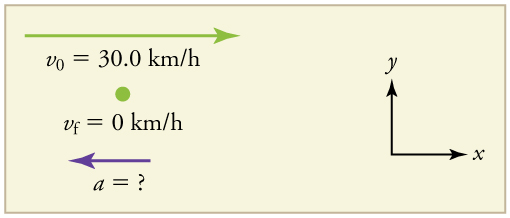
\includegraphics{images/Figure_02_03_03d.jpg}

In this case, the train is decelerating and its acceleration is negative
because it is toward the left. As in the previous example, we must find
the change in velocity and the change in time and then solve for
acceleration.

\begin{tinysection}

{Solution}

\end{tinysection}

1. Identify the knowns. \({{v_{0} = \text{30}}\text{.0\ km/h}}{}\),
\({v_{f} = 0\ km/h}{}\) (the train is stopped, so its velocity is 0), and
\({\Delta t =}\text{8.00\ s}\).

2. Solve for the change in velocity, \({\Delta v}{}\).

\leavevmode\hypertarget{import-auto-id2586229}{}%
\[{{\Delta v = {v_{f} - v_{0}}} = 0 - \text{30}}\text{.}{\text{0\ km/h} = {- \text{30}}}\text{.0\ km/h}\]

3. Plug in the knowns, \({\Delta v}{}\) and \({\Delta t}{}\), and solve for
\(\overset{-}{a}{}\).

\leavevmode\hypertarget{import-auto-id2412874}{}%
\[{{\overset{-}{a} = \frac{\Delta v}{\Delta t}} = \frac{{- \text{30}}\text{.}\text{0\ km/h}}{8\text{.}\text{00\ s}}}{}\]

4. Convert the units to meters and seconds.

\leavevmode\hypertarget{import-auto-id2596926}{}%
\[{{{\overset{-}{a} = \frac{\Delta v}{\Delta t}} = \left( \frac{- \text{30.0\ km/h}}{\text{8.00\ s}} \right)}\left( \frac{\text{10}^{3}\ \text{m}}{\text{1\ km}} \right){\left( \frac{\text{1\ h}}{\text{3600\ s}} \right) = \text{−1.04\ m/s}^{2}}}\text{.}\]

\begin{tinysection}

{Discussion}

\end{tinysection}

The minus sign indicates that acceleration is to the left. This sign is
reasonable because the train initially has a positive velocity in this
problem, and a negative acceleration would oppose the motion. Again,
acceleration is in the same direction as the \emph{change} in velocity, which
is negative here. This acceleration can be called a deceleration because
it has a direction opposite to the velocity.

The graphs of position, velocity, and acceleration vs.~time for the
trains in \protect\hyperlink{fs-id1372721}{link} and
\protect\hyperlink{fs-id3600466}{link} are displayed in
\protect\hyperlink{import-auto-id2596938}{link}. (We have taken
the velocity to remain constant from 20 to 40 s, after which the train
decelerates.)

\begin{figure}
\hypertarget{import-auto-id2596938}{%
\centering
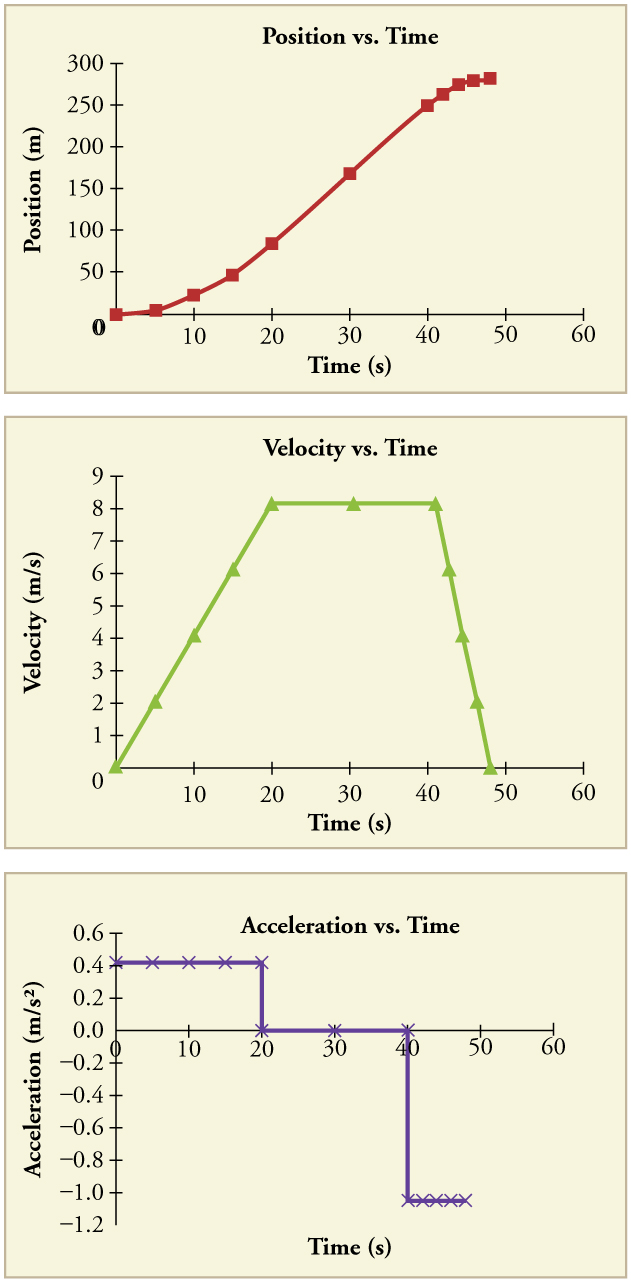
\includegraphics{images/Figure_02_03_04.jpg}
\caption{(a) Position of the train over time. Notice that the train's position
changes slowly at the beginning of the journey, then more and more
quickly as it picks up speed. Its position then changes more slowly as
it slows down at the end of the journey. In the middle of the journey,
while the velocity remains constant, the position changes at a constant
rate. (b) Velocity of the train over time. The train's velocity
increases as it accelerates at the beginning of the journey. It remains
the same in the middle of the journey (where there is no acceleration).
It decreases as the train decelerates at the end of the journey. (c) The
acceleration of the train over time. The train has positive acceleration
as it speeds up at the beginning of the journey. It has no acceleration
as it travels at constant velocity in the middle of the journey. Its
acceleration is negative as it slows down at the end of the
journey.}\label{import-auto-id2596938}
}
\end{figure}

\hypertarget{fs-id1348757}{}
Calculating Average Velocity: The Subway Train

What is the average velocity of the train in part b of
\protect\hyperlink{fs-id1744930}{link}, and shown again below, if
it takes 5.00 min to make its trip?

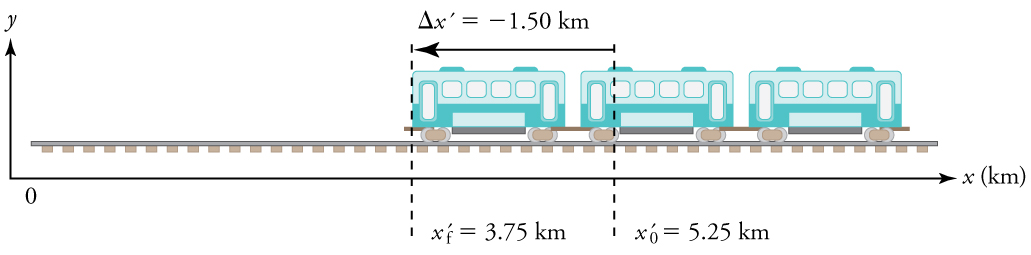
\includegraphics{images/Figure_02_03_04a.jpg}

\begin{tinysection}

{Strategy}

\end{tinysection}

Average velocity is displacement divided by time. It will be negative
here, since the train moves to the left and has a negative displacement.

\begin{tinysection}

{Solution}

\end{tinysection}

1. Identify the knowns. \({{x\prime}_{f} = 3}\text{.75\ km}\),
\({{x\prime}_{0} =}\text{5.25\ km}\), \({{\Delta t =}\text{5.00\ min}}{}\).

2. Determine displacement, \(\Delta x\prime\). We found \(\Delta x\prime\)
to be \({- \text{1.5\ km}}{}\) in
\protect\hyperlink{fs-id1744930}{link}.

3. Solve for average velocity.

\leavevmode\hypertarget{import-auto-id2338961}{}%
\[{\overset{-}{v} = \frac{\Delta x\prime}{\Delta t}} = \frac{- \text{1.50\ km}}{\text{5.00\ min}}\]

4. Convert units.

\leavevmode\hypertarget{import-auto-id2338968}{}%
\[{{\overset{-}{v} = \frac{\Delta x\prime}{\Delta t}} = \left( \frac{{- 1}\text{.}\text{50\ km}}{5\text{.}\text{00\ min}} \right)}{\left( \frac{\text{60\ min}}{1\ h} \right) = {- \text{18}}}\text{.0\ km/h}\]

\begin{tinysection}

{Discussion}

\end{tinysection}

The negative velocity indicates motion to the left.

\hypertarget{fs-id4015260}{}
Calculating Deceleration: The Subway Train

Finally, suppose the train in
\protect\hyperlink{import-auto-id2412190}{link} slows to a stop
from a velocity of 20.0 km/h in 10.0 s. What is its average
acceleration?

\begin{tinysection}

{Strategy}

\end{tinysection}

Once again, let's draw a sketch:

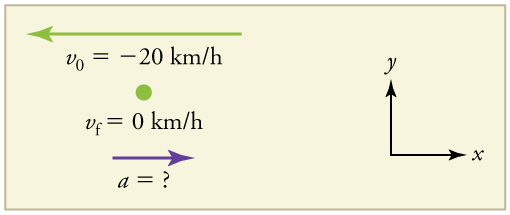
\includegraphics{images/Figure_02_03_04b.jpg}

As before, we must find the change in velocity and the change in time to
calculate average acceleration.

\begin{tinysection}

{Solution}

\end{tinysection}

1. Identify the knowns. \(v_{0} = {- \text{20\ km/h}}\),
\(v_{f} = 0\ km/h\), \({{\Delta t = \text{10}}\text{.}0\ s}{}\).

2. Calculate \({\Delta v}{}\). The change in velocity here is actually
positive, since

\leavevmode\hypertarget{import-auto-id2581122}{}%
\[{{{{\Delta v = {v_{f} - v_{0}}} = {0 - \left( {- \text{20\ km/h}} \right)}}\text{=}\text{+}\text{20\ km/h}}.}{}\]

3. Solve for \(\overset{-}{a}{}\).

\leavevmode\hypertarget{import-auto-id2585925}{}%
\[{\overset{-}{a} = \frac{\Delta v}{\Delta t}} = \frac{{+ \text{20}}\text{.0\ km/h}}{\text{10}\text{.}0\ s}\]

4. Convert units.

\leavevmode\hypertarget{import-auto-id2581171}{}%
\[{\overset{-}{a} = \left( \frac{{+ \text{20}}\text{.}\text{0\ km/h}}{\text{10}\text{.}\text{0\ s}} \right)}\left( \frac{\text{10}^{3}\ m}{1\ km} \right)\left( \frac{1\ h}{\text{3600\ s}} \right)\text{=}\ \text{+}0\text{.556\ m}\text{/s}^{2}\]

\begin{tinysection}

{Discussion}

\end{tinysection}

The plus sign means that acceleration is to the right. This is
reasonable because the train initially has a negative velocity (to the
left) in this problem and a positive acceleration opposes the motion
(and so it is to the right). Again, acceleration is in the same
direction as the \emph{change} in velocity, which is positive here. As in
\protect\hyperlink{fs-id3600466}{link}, this acceleration can be
called a deceleration since it is in the direction opposite to the
velocity.

\hypertarget{fs-id1810991}{}
\hypertarget{sign-and-direction}{%
\subsection{Sign and Direction}\label{sign-and-direction}}

Perhaps the most important thing to note about these examples is the
signs of the answers. In our chosen coordinate system, plus means the
quantity is to the right and minus means it is to the left. This is easy
to imagine for displacement and velocity. But it is a little less
obvious for acceleration. Most people interpret negative acceleration as
the slowing of an object. This was not the case in
\protect\hyperlink{fs-id4015260}{link}, where a positive
acceleration slowed a negative velocity. The crucial distinction was
that the acceleration was in the opposite direction from the velocity.
In fact, a negative acceleration will \emph{increase} a negative velocity.
For example, the train moving to the left in
\protect\hyperlink{import-auto-id2412190}{link} is sped up by an
acceleration to the left. In that case, both \(v{}\) and \(a{}\) are
negative. The plus and minus signs give the directions of the
accelerations. If acceleration has the same sign as the velocity, the
object is speeding up. If acceleration has the opposite sign as the
velocity, the object is slowing down.

\hypertarget{fs-id4121834}{}
Check Your Understanding

\leavevmode\hypertarget{fs-id4019138}{}%
An airplane lands on a runway traveling east. Describe its acceleration.

\leavevmode\hypertarget{fs-id4071605}{}%
If we take east to be positive, then the airplane has negative
acceleration, as it is accelerating toward the west. It is also
decelerating: its acceleration is opposite in direction to its velocity.

\hypertarget{fs-id4128084}{}
\begin{note}

Moving Man Simulation

Learn about position, velocity, and acceleration graphs. Move the little
man back and forth with the mouse and plot his motion. Set the position,
velocity, or acceleration and let the simulation move the man for you.
{\hfill\break
}

\hypertarget{MovingMan}{}

\end{note}

\hypertarget{fs-id4131829-summary}{}
\hypertarget{section-summary-3}{%
\subsection{Section Summary}\label{section-summary-3}}

\begin{itemize}
\item
  \protect\hypertarget{import-auto-id2412645}{}{Acceleration is the rate at which velocity changes. In symbols,
  {average acceleration} \(\overset{-}{a}{}\)
  is}
  ::: \{\#import-auto-id2412659 data-type=``equation''\}
  \[{{{\overset{-}{a} = \frac{\Delta v}{\Delta t}} = \frac{v_{f} - v_{0}}{t_{f} - t_{0}}}\text{.}}{}\]

  :::
\item
  \protect\hypertarget{import-auto-id2412738}{}{The SI unit for acceleration is
  \(\text{m/s}^{2}{}\).}
\item
  \protect\hypertarget{import-auto-id2412758}{}{Acceleration is a vector, and thus has a both a magnitude and
  direction.}
\item
  \protect\hypertarget{import-auto-id2412770}{}{Acceleration can be caused by either a change in the magnitude or
  the direction of the velocity.}
\item
  \protect\hypertarget{import-auto-id2412772}{}{Instantaneous acceleration \(a{}\) is the acceleration at a specific
  instant in time.}
\item
  \protect\hypertarget{import-auto-id2412729}{}{Deceleration is an acceleration with a direction opposite to that
  of the velocity.}
\end{itemize}

\hypertarget{fs-id3526388}{}
\begin{conceptual-questions}

\hypertarget{conceptual-questions-3}{%
\subsection{Conceptual Questions}\label{conceptual-questions-3}}

\hypertarget{fs-id3526394}{}
\leavevmode\hypertarget{fs-id3526396}{}%
Is it possible for speed to be constant while acceleration is not zero?
Give an example of such a situation.

\hypertarget{fs-id4016173}{}
\leavevmode\hypertarget{fs-id4016175}{}%
Is it possible for velocity to be constant while acceleration is not
zero? Explain.

\hypertarget{fs-id3514238}{}
\leavevmode\hypertarget{fs-id3514240}{}%
Give an example in which velocity is zero yet acceleration is not.

\hypertarget{fs-id1765962}{}
\leavevmode\hypertarget{fs-id1765964}{}%
If a subway train is moving to the left (has a negative velocity) and
then comes to a stop, what is the direction of its acceleration? Is the
acceleration positive or negative?

\hypertarget{fs-id1780345}{}
\leavevmode\hypertarget{fs-id1780347}{}%
Plus and minus signs are used in one-dimensional motion to indicate
direction. What is the sign of an acceleration that reduces the
magnitude of a negative velocity? Of a positive velocity?

\end{conceptual-questions}

\hypertarget{fs-id4129894}{}
\begin{problems-exercises}

\hypertarget{problems-exercises-2}{%
\subsection{Problems \& Exercises}\label{problems-exercises-2}}

\hypertarget{fs-id4129901}{}
\leavevmode\hypertarget{fs-id4129903}{}%
A cheetah can accelerate from rest to a speed of 30.0 m/s in 7.00 s.
What is its acceleration?

\leavevmode\hypertarget{fs-id4059926}{}%
\({4\text{.}\text{29}\ \text{m/s}^{2}}{}\)

\hypertarget{fs-id4035192}{}
\hypertarget{fs-id4035194}{}
\begin{tinysection}

{Professional Application}

\end{tinysection}

Dr.~John Paul Stapp was U.S. Air Force officer who studied the effects
of extreme deceleration on the human body. On December 10, 1954, Stapp
rode a rocket sled, accelerating from rest to a top speed of 282 m/s
(1015 km/h) in 5.00 s, and was brought jarringly back to rest in only
1.40 s! Calculate his (a) acceleration and (b) deceleration. Express
each in multiples of \(g{}\) \({(9\text{.}\text{80\ m}\text{/s}^{2})}{}\) by
taking its ratio to the acceleration of gravity.

\hypertarget{fs-id2299988}{}
\leavevmode\hypertarget{fs-id2299990}{}%
A commuter backs her car out of her garage with an acceleration of
\({1\text{.}\text{40\ m/s}^{2}}{}\). (a) How long does it take her to
reach a speed of 2.00 m/s? (b) If she then brakes to a stop in 0.800 s,
what is her deceleration?

\leavevmode\hypertarget{fs-id4124023}{}%
\(a\) \({1\text{.}\text{43\ s}}{}\)

\(b\) \({{- 2}\text{.}\text{50}\ \text{m/s}^{2}}{}\)

\hypertarget{fs-id4124470}{}
\leavevmode\hypertarget{fs-id4124472}{}%
Assume that an intercontinental ballistic missile goes from rest to a
suborbital speed of 6.50 km/s in 60.0 s (the actual speed and time are
classified). What is its average acceleration in \(\text{m/s}^{2}{}\) and
in multiples of \(g{}\) \({{(9\text{.}\text{80\ m}\text{/s}^{2})}?}{}\)

\end{problems-exercises}

\hypertarget{fs-id1922895}{}
\begin{ap-test-prep}

\hypertarget{test-prep-for-ap-courses-3}{%
\subsection{Test Prep for AP Courses}\label{test-prep-for-ap-courses-3}}

\hypertarget{fs-id1454119}{}
\leavevmode\hypertarget{fs-id3184331}{}%
\begin{figure}
\hypertarget{fs-id3184333}{%
\centering
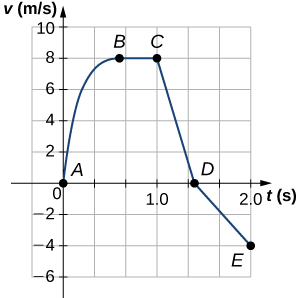
\includegraphics{images/Figure_Ch2_M4_14.jpg}
\caption{Graph showing Velocity vs.~Time of a
cart.}\label{fs-id3184333}
}
\end{figure}

A cart is constrained to move along a straight line. A varying net force
along the direction of motion is exerted on the cart. The cart's
velocity \emph{v} as a function of time \emph{t} is shown in the graph. The five
labeled points divide the graph into four sections.

Which of the following correctly ranks the magnitude of the average
acceleration of the cart during the four sections of the graph?

\begin{enumerate}
\def\labelenumi{\alph{enumi}.}
\tightlist
\item
  \emph{a\textsubscript{CD}} \textgreater{} \emph{a\textsubscript{AB}} \textgreater{} \emph{a\textsubscript{BC}} \textgreater{} \emph{a\textsubscript{DE}}
\item
  \emph{a\textsubscript{BC}} \textgreater{} \emph{a\textsubscript{AB}} \textgreater{} \emph{a\textsubscript{CD}} \textgreater{} \emph{a\textsubscript{DE}}
\item
  \emph{a\textsubscript{AB}} \textgreater{} \emph{a\textsubscript{BC}} \textgreater{} \emph{a\textsubscript{DE}} \textgreater{} \emph{a\textsubscript{CD}}
\item
  \emph{a\textsubscript{CD}} \textgreater{} \emph{a\textsubscript{AB}} \textgreater{} \emph{a\textsubscript{DE}} \textgreater{} \emph{a\textsubscript{BC}}
\end{enumerate}

\hypertarget{fs-id1860126}{}
\leavevmode\hypertarget{fs-id2388387}{}%
Push a book across a table and observe it slow to a stop.

Draw graphs showing the book's position vs.~time and velocity vs.~time
if the direction of its motion is considered positive.

Draw graphs showing the book's position vs.~time and velocity vs.~time
if the direction of its motion is considered negative.

\leavevmode\hypertarget{fs-id2548115}{}%
The position vs.~time graph should be represented with a positively
sloped line whose slope steadily decreases to zero. The \emph{y}-intercept of
the graph may be any value. The line on the velocity vs.~time graph
should have a positive \emph{y}-intercept and a negative slope. Because the
final velocity of the book is zero, the line should finish on the
\emph{x}-axis.

The position vs.~time graph should be represented with a negatively
sloped line whose slope steadily decreases to zero. The \emph{y}-intercept of
the graph may be any value. The line on the velocity vs.~time graph
should have a negative \emph{y}-intercept and a positive slope. Because the
final velocity of the book is zero, the line should finish on the
\emph{x}-axis.{]}

\end{ap-test-prep}

\hypertarget{glossary-3}{%
\subsection{Glossary}\label{glossary-3}}

\begin{description}
\tightlist
\item[acceleration]
the rate of change in velocity; the change in velocity over time
\end{description}

\begin{description}
\tightlist
\item[average acceleration]
the change in velocity divided by the time over which it changes
\end{description}

\begin{description}
\tightlist
\item[instantaneous acceleration]
acceleration at a specific point in time
\end{description}

\begin{description}
\tightlist
\item[deceleration]
acceleration in the direction opposite to velocity; acceleration
that results in a decrease in velocity
\end{description}

\hypertarget{motion-equations-for-constant-acceleration-in-one-dimension}{%
\section{Motion Equations for Constant Acceleration in One Dimension}\label{motion-equations-for-constant-acceleration-in-one-dimension}}

\begin{figure}
\hypertarget{import-auto-id1489960}{%
\centering
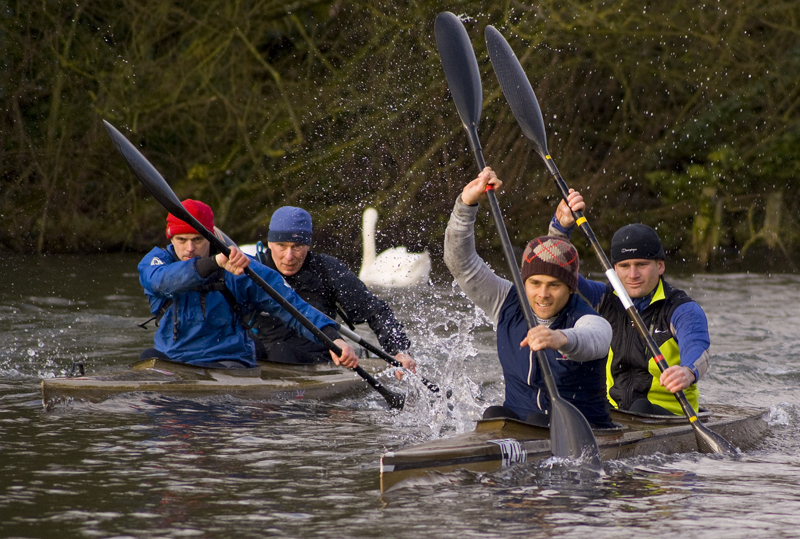
\includegraphics{images/Figure_02_05_00.jpg}
\caption{Kinematic equations can help us describe and predict the motion of
moving objects such as these kayaks racing in Newbury, England. (credit:
Barry Skeates,
Flickr)}\label{import-auto-id1489960}
}
\end{figure}

\hypertarget{fs-id1547877}{}
\begin{learning-objectives}

\hypertarget{learning-objectives-3}{%
\subsection{Learning Objectives}\label{learning-objectives-3}}

By the end of this section, you will be able to:

\begin{itemize}
\tightlist
\item
  Calculate displacement of an object that is not accelerating, given
  initial position and velocity.
\item
  Calculate final velocity of an accelerating object, given initial
  velocity, acceleration, and time.
\item
  Calculate displacement and final position of an accelerating object,
  given initial position, initial velocity, time, and acceleration.
\end{itemize}

The information presented in this section supports the following AP®
learning objectives and science practices:

\begin{itemize}
\tightlist
\item
  \textbf{3.A.1.1} The student is able to express the motion of an object
  using narrative, mathematical, or graphical representations. \textbf{(S.P.
  1.5, 2.1, 2.2)}
\item
  \textbf{3.A.1.3} The student is able to analyze experimental data
  describing the motion of an object and is able to express the
  results of the analysis using narrative, mathematical, and graphical
  representations. \textbf{(S.P. 5.1)}
\end{itemize}

\end{learning-objectives}

We might know that the greater the acceleration of, say, a car moving
away from a stop sign, the greater the displacement in a given time. But
we have not developed a specific equation that relates acceleration and
displacement. In this section, we develop some convenient equations for
kinematic relationships, starting from the definitions of displacement,
velocity, and acceleration already covered.

\hypertarget{fs-id1164906436587}{}
\hypertarget{notation-t-x-v-a}{%
\subsection{\texorpdfstring{Notation: \emph{t}, \emph{x}, \emph{v}, \emph{a}}{Notation: t, x, v, a}}\label{notation-t-x-v-a}}

First, let us make some simplifications in notation. Taking the initial
time to be zero, as if time is measured with a stopwatch, is a great
simplification. Since elapsed time is \({\Delta t = {t_{f} - t_{0}}}{}\),
taking \({t_{0} = 0}{}\) means that \({\Delta t = t_{f}}{}\), the final time
on the stopwatch. When initial time is taken to be zero, we use the
subscript 0 to denote initial values of position and velocity. That is,
\(x_{0}\) \emph{is the initial position} and \(v_{0}{}\) \emph{is the initial
velocity}. We put no subscripts on the final values. That is, \(t\) \emph{is
the final time}, \(x{}\) \emph{is the final position}, and \(v\) \emph{is the final
velocity}. This gives a simpler expression for elapsed time---now,
\({\Delta t = t}{}\). It also simplifies the expression for displacement,
which is now \(\Delta x = {x - x_{0}}\). Also, it simplifies the
expression for change in velocity, which is now
\({\Delta v = {v - v_{0}}}{}\). To summarize, using the simplified
notation, with the initial time taken to be zero,

\leavevmode\hypertarget{import-auto-id2563693}{}%
\[\left. \begin{array}{lll}
{\Delta t} & = & t \\
{\Delta x} & = & {x - x_{0}} \\
{\Delta v} & = & {v - v_{0}} \\
\end{array} \right\}\]

where \emph{the subscript 0 denotes an initial value and the absence of a
subscript denotes a final value} in whatever motion is under
consideration.

We now make the important assumption that \emph{acceleration is constant}.
This assumption allows us to avoid using calculus to find instantaneous
acceleration. Since acceleration is constant, the average and
instantaneous accelerations are equal. That is,

\leavevmode\hypertarget{import-auto-id1819116}{}%
\[{{{\overset{-}{a} = a} = \text{constant}},}{}\]

so we use the symbol \(a{}\) for acceleration at all times. Assuming
acceleration to be constant does not seriously limit the situations we
can study nor degrade the accuracy of our treatment. For one thing,
acceleration \emph{is} constant in a great number of situations. Furthermore,
in many other situations we can accurately describe motion by assuming a
constant acceleration equal to the average acceleration for that motion.
Finally, in motions where acceleration changes drastically, such as a
car accelerating to top speed and then braking to a stop, the motion can
be considered in separate parts, each of which has its own constant
acceleration.

\hypertarget{fs-id1164906424651}{}
\begin{note}

Solving for Displacement (\(\Delta x\)) and Final Position (\(x{}\)) from
Average Velocity when Acceleration (\(a{}\)) is Constant

To get our first two new equations, we start with the definition of
average velocity:

\leavevmode\hypertarget{import-auto-id1782525}{}%
\[{{\overset{-}{v} = \frac{\Delta x}{\Delta t}}\text{.}}{}\]

Substituting the simplified notation for \(\Delta x\) and \(\Delta t\)
yields

\leavevmode\hypertarget{import-auto-id4145482}{}%
\[{{\overset{-}{v} = \frac{x - x_{0}}{t}}\text{.}}{}\]

Solving for \(x{}\) yields

\leavevmode\hypertarget{import-auto-id2297251}{}%
\[{{x = {x_{0} + \overset{-}{v}}}t\text{,}}{}\]

where the average velocity is

\leavevmode\hypertarget{import-auto-id2086556}{}%
\[{{\overset{-}{v} = \frac{v_{0} + v}{2}}\ (\text{constant}\ a)\text{.}}{}\]

\end{note}

The equation \({\overset{-}{v} = \frac{v_{0} + v}{2}}{}\) reflects the
fact that, when acceleration is constant, \(v{}\) is just the simple
average of the initial and final velocities. For example, if you
steadily increase your velocity (that is, with constant acceleration)
from 30 to 60 km/h, then your average velocity during this steady
increase is 45 km/h. Using the equation
\({\overset{-}{v} = \frac{v_{0} + v}{2}}{}\) to check this, we see that

\leavevmode\hypertarget{import-auto-id4152098}{}%
\[{{{\overset{-}{v} = \frac{v_{0} + v}{2}} = \frac{\text{30\ km/h} + \text{60\ km/h}}{2}} = \text{45\ km/h,}}{}\]

which seems logical.

\hypertarget{fs-id1164906442368}{}
Calculating Displacement: How Far does the Jogger Run?

A jogger runs down a straight stretch of road with an average velocity
of 4.00 m/s for 2.00 min. What is his final position, taking his initial
position to be zero?

\begin{tinysection}

{Strategy}

\end{tinysection}

Draw a sketch.

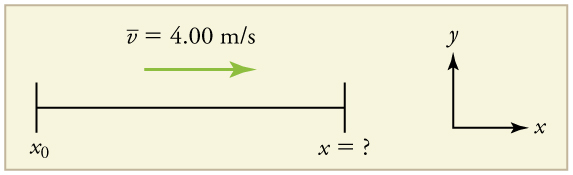
\includegraphics{images/Figure_02_05_00a.jpg}

The final position \(x{}\) is given by the equation

\leavevmode\hypertarget{import-auto-id2168543}{}%
\[{{{x = {x_{0} + \overset{-}{v}}}t}.}{}\]

To find \(x{}\), we identify the values of \(x_{0}{}\),
\emph{\(\overset{-}{v}{}\)}, and \(t{}\)\emph{} from the
statement of the problem and substitute them into the equation.

\begin{tinysection}

{Solution}

\end{tinysection}

1. Identify the knowns.
\({{\overset{-}{v} = 4}\text{.}\text{00\ m/s}}{}\),
\({{\Delta t = 2}\text{.}\text{00\ min}}{}\), and
\({x_{0} = \text{0\ m}}{}\).\emph{}

2. Enter the known values into the equation.

\leavevmode\hypertarget{import-auto-id2300752}{}%
\[{{x = {x_{0} + \overset{-}{v}}}{t = {0 + \left( {4\text{.}\text{00\ m/s}} \right)}}{\left( \text{120\ s} \right) = \text{480\ m}}}{}\]

\begin{tinysection}

{Discussion}

\end{tinysection}

Velocity and final displacement are both positive, which means they are
in the same direction.

The equation \({{x = {x_{0} + \overset{-}{v}}}t}{}\) gives insight into
the relationship between displacement, average velocity, and time. It
shows, for example, that displacement is a linear function of average
velocity. (By linear function, we mean that displacement depends on
\emph{\(\overset{-}{v}{}\)} rather than on \emph{\(\overset{-}{v}{}\)} raised to some
other power, such as \emph{\({\overset{-}{v}}^{2}{}\)}. When graphed, linear
functions look like straight lines with a constant slope.) On a car
trip, for example, we will get twice as far in a given time if we
average 90 km/h than if we average 45 km/h.

\begin{figure}
\hypertarget{import-auto-id1962019}{%
\centering
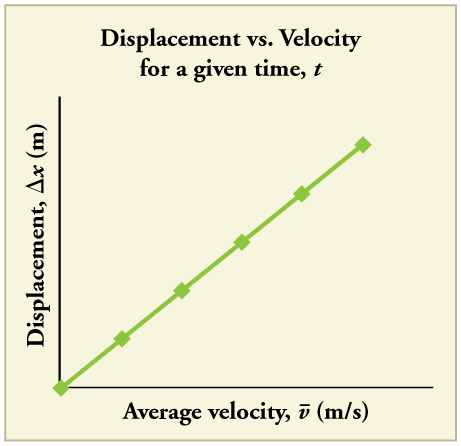
\includegraphics{images/Figure_02_05_00b.jpg}
\caption{There is a linear relationship between displacement and average
velocity. For a given time \(t{}\), an object moving twice as fast as
another object will move twice as far as the other
object.}\label{import-auto-id1962019}
}
\end{figure}

\hypertarget{fs-id1164906431223}{}
\begin{note}

Solving for Final Velocity

We can derive another useful equation by manipulating the definition of
acceleration.

\leavevmode\hypertarget{import-auto-id2366011}{}%
\[a = \frac{\Delta v}{\Delta t}\]

Substituting the simplified notation for \({\Delta v}{}\) and \(\Delta t\)
gives us

\leavevmode\hypertarget{import-auto-id1962571}{}%
\[{{a = \frac{v - v_{0}}{t}}\ (\text{constant}\ a)\text{.}}{}\]

Solving for \(v{}\) yields

\leavevmode\hypertarget{import-auto-id2168495}{}%
\[{{v = {v_{0} + \text{at}}}\ (\text{constant}\ a)\text{.}}{}\]

\end{note}

\hypertarget{fs-id1164906431414}{}
Calculating Final Velocity: An Airplane Slowing Down after Landing

An airplane lands with an initial velocity of 70.0 m/s and then
decelerates at \({1\text{.}\text{50\ m/s}^{2}}{}\) for 40.0 s. What is its
final velocity?

\begin{tinysection}

{Strategy}

\end{tinysection}

Draw a sketch. We draw the acceleration vector in the direction opposite
the velocity vector because the plane is decelerating.

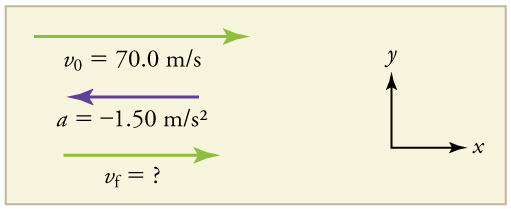
\includegraphics{images/Figure_02_05_00c.jpg}

\begin{tinysection}

{Solution}

\end{tinysection}

1. Identify the knowns. \({{v_{0} = \text{70}}\text{.}\text{0\ m/s}}{}\),
\({{a = {- 1}}\text{.}\text{50\ m/s}^{2}}{}\),
\({{t = \text{40}}\text{.}0\ \text{s}}{}\).

2. Identify the unknown. In this case, it is final velocity,
\(v_{f}{}\)\textsubscript{.}

3. Determine which equation to use. We can calculate the final velocity
using the equation \({v = {v_{0} + \text{at}}}{}\).

4. Plug in the known values and solve.

\leavevmode\hypertarget{import-auto-id2177855}{}%
\[{{{v = {v_{0} + \text{at}}} = \text{70}}\text{.}{\text{0\ m/s} + \left( {{- 1}\text{.}\text{50\ m/s}^{2}} \right)}{\left( {\text{40}\text{.}\text{0\ s}} \right) = \text{10}}\text{.}\text{0\ m/s}}{}\]

\begin{tinysection}

{Discussion}

\end{tinysection}

The final velocity is much less than the initial velocity, as desired
when slowing down, but still positive. With jet engines, reverse thrust
could be maintained long enough to stop the plane and start moving it
backward. That would be indicated by a negative final velocity, which is
not the case here.

\begin{figure}
\hypertarget{import-auto-id2173965}{%
\centering
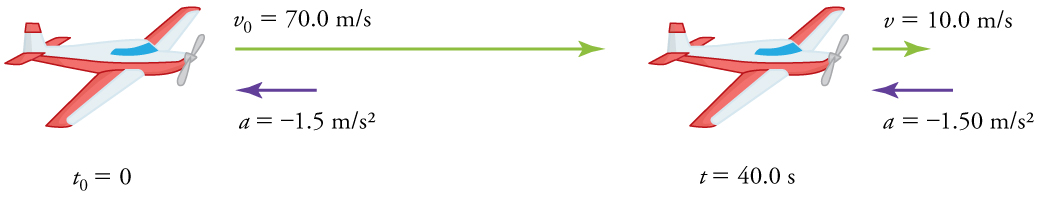
\includegraphics{images/Figure_02_04_01.jpg}
\caption{The airplane lands with an initial velocity of 70.0 m/s and slows to a
final velocity of 10.0 m/s before heading for the terminal. Note that
the acceleration is negative because its direction is opposite to its
velocity, which is
positive.}\label{import-auto-id2173965}
}
\end{figure}

In addition to being useful in problem solving, the equation
\({v = {v_{0} + \text{at}}}{}\) gives us insight into the relationships
among velocity, acceleration, and time. From it we can see, for example,
that

\begin{itemize}
\tightlist
\item
  \protect\hypertarget{import-auto-id2180047}{}{final velocity depends on how large the acceleration is and how
  long it lasts}
\item
  \protect\hypertarget{import-auto-id2180050}{}{if the acceleration is zero, then the final velocity equals the
  initial velocity \({({v = v_{0}})}{}\), as expected (i.e., velocity is
  constant)}
\item
  \protect\hypertarget{import-auto-id2175665}{}{if \emph{\(a{}\)} is negative, then the final velocity is less than the
  initial velocity}
\end{itemize}

(All of these observations fit our intuition, and it is always useful to
examine basic equations in light of our intuition and experiences to
check that they do indeed describe nature accurately.)

\hypertarget{fs-id1164906437247}{}
\begin{note}

Making Connections: Real-World Connection

{\hfill\break
}

\begin{figure}
\hypertarget{import-auto-id2180893}{%
\centering
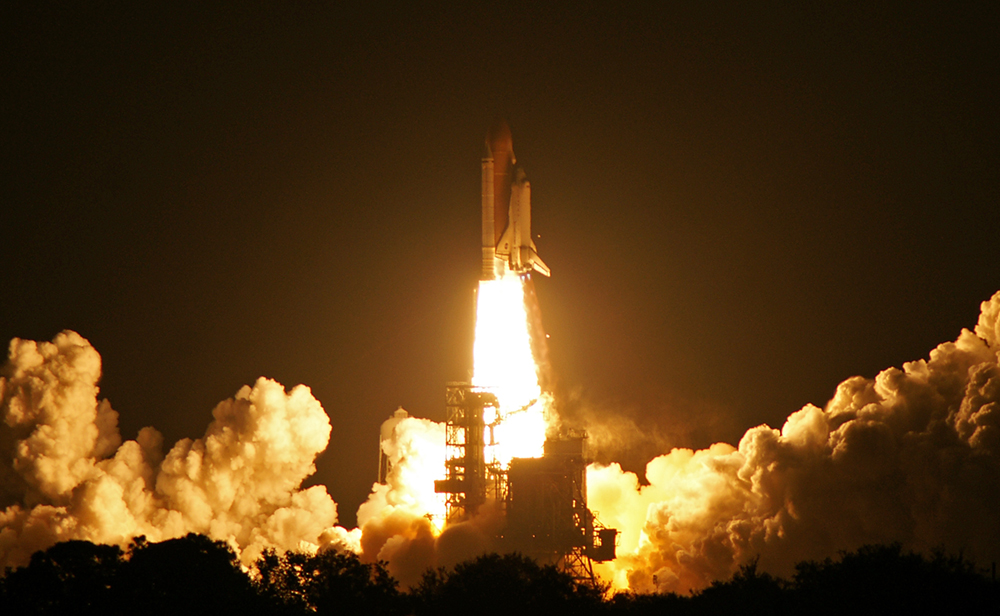
\includegraphics{images/Figure_02_04_01a.jpg}
\caption{The Space Shuttle \emph{Endeavor} blasts off from the Kennedy Space Center
in February 2010. (credit: Matthew Simantov,
Flickr)}\label{import-auto-id2180893}
}
\end{figure}

An intercontinental ballistic missile (ICBM) has a larger average
acceleration than the Space Shuttle and achieves a greater velocity in
the first minute or two of flight (actual ICBM burn times are
classified---short-burn-time missiles are more difficult for an enemy to
destroy). But the Space Shuttle obtains a greater final velocity, so
that it can orbit the earth rather than come directly back down as an
ICBM does. The Space Shuttle does this by accelerating for a longer
time.

\end{note}

\hypertarget{fs-id1164906444525}{}
\begin{note}

Solving for Final Position When Velocity is Not Constant (\(a \neq 0\))

We can combine the equations above to find a third equation that allows
us to calculate the final position of an object experiencing constant
acceleration. We start with

\leavevmode\hypertarget{import-auto-id2166975}{}%
\[{v = {v_{0} + \text{at}}.}{}\]

Adding \(v_{0}{}\) to each side of this equation and dividing by 2 gives

\leavevmode\hypertarget{import-auto-id1689620}{}%
\[{{\frac{v_{0} + v}{2} = {v_{0} + \frac{1}{2}}}\text{at}\text{.}}{}\]

Since \({\frac{v_{0} + v}{2} = \overset{-}{v}}{}\) for constant
acceleration, then

\leavevmode\hypertarget{import-auto-id2301379}{}%
\[{{\overset{-}{v} = {v_{0} + \frac{1}{2}}}\text{at}\text{.}}{}\]

Now we substitute this expression for \(\overset{-}{v}{}\) into the
equation for displacement, \({{x = {x_{0} + \overset{-}{v}}}t}{}\),
yielding

\leavevmode\hypertarget{import-auto-id1807031}{}%
\[{{x = {x_{0} + v_{0}}}{t + \frac{1}{2}}\text{at}^{2}\ (\text{constant}\ a)\text{.}}{}\]

\end{note}

\hypertarget{fs-id1164906457202}{}
Calculating Displacement of an Accelerating Object: Dragsters

Dragsters can achieve average accelerations of
\({\text{26}\text{.}\text{0\ m/s}^{2}}{}\). Suppose such a dragster
accelerates from rest at this rate for 5.56 s. How far does it travel in
this time?

\begin{figure}
\hypertarget{import-auto-id2356722}{%
\centering
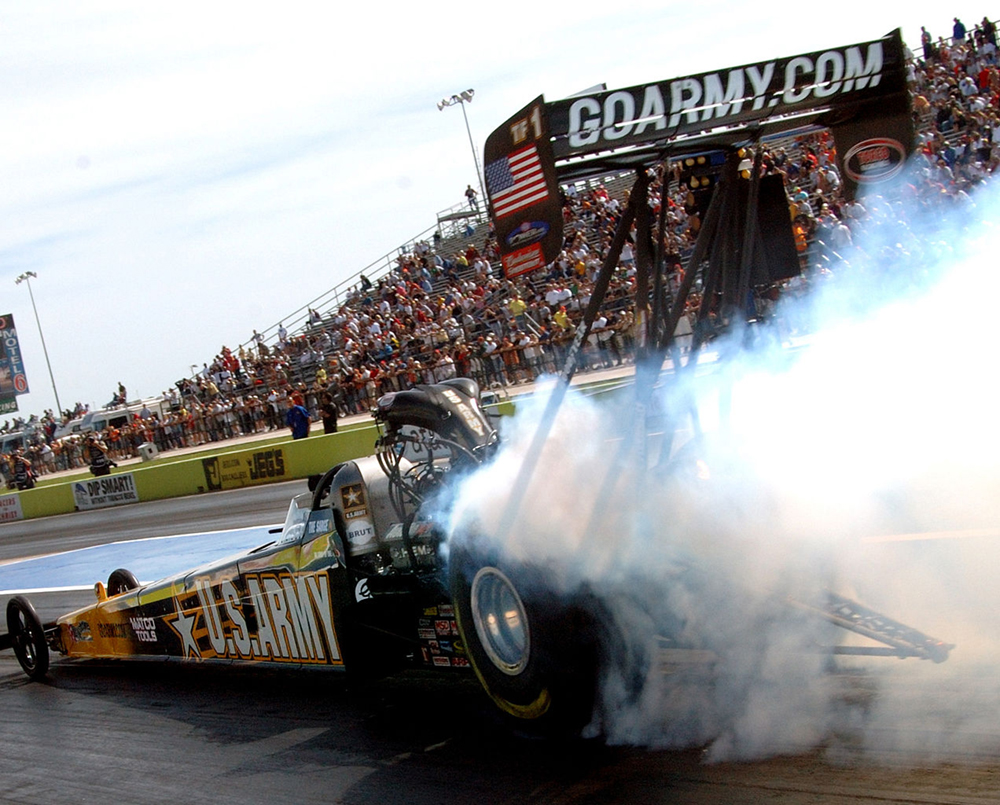
\includegraphics{images/Figure_02_04_02.jpg}
\caption{U.S. Army Top Fuel pilot Tony ``The Sarge'' Schumacher begins a race
with a controlled burnout. (credit: Lt. Col. William Thurmond. Photo
Courtesy of U.S.
Army.)}\label{import-auto-id2356722}
}
\end{figure}

\begin{tinysection}

{Strategy}

\end{tinysection}

Draw a sketch.

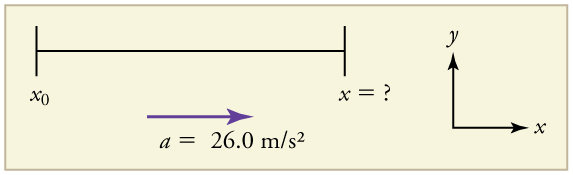
\includegraphics{images/Figure_02_04_02a.jpg}

We are asked to find displacement, which is \(x\) if we take \(x_{0}{}\) to
be zero. (Think about it like the starting line of a race. It can be
anywhere, but we call it 0 and measure all other positions relative to
it.) We can use the equation
\({{x = {x_{0} + v_{0}}}{t + \frac{1}{2}}\text{at}^{2}}{}\)\emph{}once
we identify \(v_{0}{}\), \(a{}\), and \(t{}\) from the statement of the
problem.

\begin{tinysection}

{Solution}

\end{tinysection}

1. Identify the knowns. \textbf{}Starting from
rest means that \({v_{0} = 0}{}\),
\emph{}\(a{}\)\emph{} is
given as \({\text{26}\text{.}0\ \text{m/s}^{2}}{}\) and
\(t{}\)\emph{} is given as 5.56 s.

2. Plug the known values into the equation to solve for the unknown
\(x{}\):

\leavevmode\hypertarget{import-auto-id2171407}{}%
\[{{x = {x_{0} + v_{0}}}{t + \frac{1}{2}}\text{at}^{2}\text{.}}{}\]

Since the initial position and velocity are both zero, this simplifies
to

\leavevmode\hypertarget{import-auto-id2171445}{}%
\[{{x = \frac{1}{2}}\text{at}^{2}\text{.}}{}\]

Substituting the identified values of \(a{}\) and \(t{}\) gives

\leavevmode\hypertarget{import-auto-id2169820}{}%
\[{{x = \frac{1}{2}}\left( {\text{26}\text{.}\text{0\ m/s}^{2}} \right)\left( {5\text{.}\text{56\ s}} \right)^{2},}{}\]

yielding

\leavevmode\hypertarget{import-auto-id2171362}{}%
\[{x = \text{402\ m.}}{}\]

\begin{tinysection}

{Discussion}

\end{tinysection}

If we convert 402 m to miles, we find that the distance covered is very
close to one quarter of a mile, the standard distance for drag racing.
So the answer is reasonable. This is an impressive displacement in only
5.56 s, but top-notch dragsters can do a quarter mile in even less time
than this.

What else can we learn by examining the equation
\({{x = {x_{0} + v_{0}}}{t + \frac{1}{2}}\text{at}^{2}}?\) We see that:

\begin{itemize}
\tightlist
\item
  \protect\hypertarget{import-auto-id2166810}{}{displacement depends on the square of the elapsed time when
  acceleration is not zero. In
  \protect\hyperlink{fs-id1164906457202}{link}, the dragster
  covers only one fourth of the total distance in the first half of
  the elapsed time}
\item
  \protect\hypertarget{import-auto-id2167534}{}{if acceleration is zero, then the initial velocity equals average
  velocity (\({v_{0} = \overset{-}{v}}{}\)) and
  \({{x = {x_{0} + v_{0}}}{t + \frac{1}{2}}\text{at}^{2}}{}\) becomes
  \({{x = {x_{0} + v_{0}}}t}{}\)}
\end{itemize}

\hypertarget{fs-id1164906460433}{}
\begin{note}

Solving for Final Velocity when Velocity Is Not Constant (\(a \neq 0\))

A fourth useful equation can be obtained from another algebraic
manipulation of previous equations.

If we solve \({v = {v_{0} + \text{at}}}{}\) for \(t{}\), we get

\leavevmode\hypertarget{import-auto-id2365760}{}%
\[{{t = \frac{v - v_{0}}{a}}\text{.}}{}\]

Substituting this and \({\overset{-}{v} = \frac{v_{0} + v}{2}}{}\) into
\({{x = {x_{0} + \overset{-}{v}}}t}{}\), we get

\leavevmode\hypertarget{import-auto-id1659227}{}%
\[{v^{2} = {v_{0}^{2} + 2a}}\left( {x - x_{0}} \right)\ (\text{constant} a)\text{.}\]

\end{note}

\hypertarget{fs-id1164906443776}{}
Calculating Final Velocity: Dragsters

Calculate the final velocity of the dragster in
\protect\hyperlink{fs-id1164906457202}{link} without using
information about time.

\begin{tinysection}

{Strategy}

\end{tinysection}

Draw a sketch.

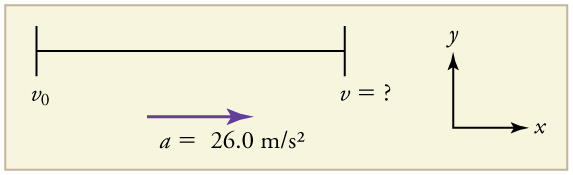
\includegraphics{images/Figure_02_04_02b.jpg}

The equation \({{v^{2} = {v_{0}^{2} + 2a}}({x - x_{0}})}{}\) is ideally
suited to this task because it relates velocities, acceleration, and
displacement, and no time information is required.

\begin{tinysection}

{Solution}

\end{tinysection}

1. Identify the known values. We know that \({v_{0} = 0}{}\), since the
dragster starts from rest. Then we note that
\({{x - x_{0}} = \text{402\ m}}{}\) (this was the answer in
\protect\hyperlink{fs-id1164906457202}{link}). Finally, the
average acceleration was given to be
\({{a = \text{26}}\text{.}\text{0\ m/s}^{2}}{}\).

2. Plug the knowns into the equation
\({v^{2} = {v_{0}^{2} + 2a}}({x - x_{0}})\) and solve for \(v.\)

\leavevmode\hypertarget{import-auto-id1680164}{}%
\[{{{v^{2} = {0 + 2}}\left( {\text{26}\text{.}\text{0\ m/s}^{2}} \right)\left( \text{402\ m} \right)}.}{}\]

Thus

\leavevmode\hypertarget{import-auto-id2177794}{}%
\[{{{v^{2} = 2}\text{.}{\text{09} \times \text{10}^{4}}\ \text{m}^{2}\text{/s}^{2}}.}{}\]

To get \(v{}\), we take the square root:

\leavevmode\hypertarget{import-auto-id2177812}{}%
\[{{v = \sqrt{2\text{.}{\text{09} \times \text{10}^{4}}\ \text{m}^{2}\text{/s}^{2}}} = \text{145\ m/s}}.\]

\begin{tinysection}

{Discussion}

\end{tinysection}

145 m/s is about 522 km/h or about 324 mi/h, but even this breakneck
speed is short of the record for the quarter mile. Also, note that a
square root has two values; we took the positive value to indicate a
velocity in the same direction as the acceleration.

An examination of the equation
\({{v^{2} = {v_{0}^{2} + 2a}}({x - x_{0}})}{}\) can produce further
insights into the general relationships among physical quantities:

\begin{itemize}
\tightlist
\item
  \protect\hypertarget{import-auto-id1680053}{}{The final velocity depends on how large the acceleration is and the
  distance over which it acts}
\item
  \protect\hypertarget{import-auto-id1680020}{}{For a fixed deceleration, a car that is going twice as fast
  doesn't simply stop in twice the distance---it takes much further
  to stop. (This is why we have reduced speed zones near
  schools.)}
\end{itemize}

\hypertarget{fs-id1164906446591}{}
\hypertarget{putting-equations-together}{%
\subsection{Putting Equations Together}\label{putting-equations-together}}

In the following examples, we further explore one-dimensional motion,
but in situations requiring slightly more algebraic manipulation. The
examples also give insight into problem-solving techniques. The box
below provides easy reference to the equations needed.

\hypertarget{fs-id1164906460309}{}
\begin{note}

Summary of Kinematic Equations (constant \(a{}\))

\leavevmode\hypertarget{import-auto-id1771742}{}%
\[{{x =}x_{0}{+}\overset{-}{v}t}{}\]

\leavevmode\hypertarget{import-auto-id4178996}{}%
\[{{\overset{-}{v} =}\frac{v_{0} + v}{2}}{}\]

\leavevmode\hypertarget{import-auto-id1680040}{}%
\[{v = {v_{0} + \text{at}}}{}\]

\leavevmode\hypertarget{import-auto-id1680037}{}%
\[{{x = {x_{0} + v_{0}}}{t + \frac{1}{2}}\text{at}^{2}}{}\]

\leavevmode\hypertarget{import-auto-id2178979}{}%
\[{{v^{2} = {v_{0}^{2} + 2a}}\left( {x - x_{0}} \right)}{}\]

\end{note}

\hypertarget{fs-id1164906424692}{}
Calculating Displacement: How Far Does a Car Go When Coming to a Halt?

On dry concrete, a car can decelerate at a rate of
\({7\text{.}\text{00\ m/s}^{2}}{}\), whereas on wet concrete it can
decelerate at only \({5\text{.}\text{00\ m/s}^{2}}{}\). Find the distances
necessary to stop a car moving at 30.0
m/s\emph{} (about 110 km/h) (a) on dry concrete
and (b) on wet concrete. (c) Repeat both calculations, finding the
displacement from the point where the driver sees a traffic light turn
red, taking into account his reaction time of 0.500 s to get his foot on
the brake.

\begin{tinysection}

{Strategy}

\end{tinysection}

Draw a sketch.

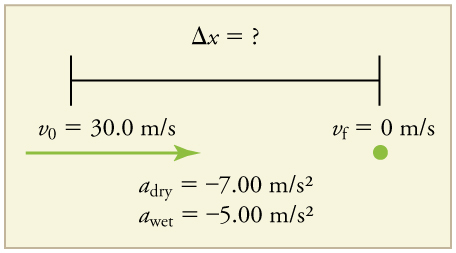
\includegraphics{images/Figure_02_04_02c.jpg}

In order to determine which equations are best to use, we need to list
all of the known values and identify exactly what we need to solve for.
We shall do this explicitly in the next several examples, using tables
to set them off.

\begin{tinysection}

{Solution for (a)}

\end{tinysection}

1. Identify the knowns and what we want to solve for. We know that
\({{v_{0} = \text{30}}\text{.}\text{0\ m/s}}{}\); \({v = \text{0}}{}\);
\({{a = {- 7}}\text{.}\text{00}\ \text{m/s}^{2}}{}\) (\(a\) is negative
because it is in a direction opposite to velocity). We take \(x_{0}{}\) to
be 0. We are looking for displacement \({\Delta x}{}\), or
\({x - x_{0}}{}\).

2. Identify the equation that will help up solve the problem. The best
equation to use is

\leavevmode\hypertarget{import-auto-id2180580}{}%
\[{{{v^{2} = {v_{0}^{2} + 2a}}\left( {x - x_{0}} \right)}.}{}\]

This equation is best because it includes only one unknown, \(x{}\). We
know the values of all the other variables in this equation. (There are
other equations that would allow us to solve for \(x{}\), but they require
us to know the stopping time, \(t{}\), which we do not know. We could use
them but it would entail additional calculations.)

3. Rearrange the equation to solve for \(x{}\).

\leavevmode\hypertarget{import-auto-id4179294}{}%
\[x - x_{0} = \frac{v^{2} - v_{0}^{2}}{2a}\]

4. Enter known values.

\leavevmode\hypertarget{import-auto-id2293184}{}%
\[{{x - 0} = \frac{0^{2} - \left( {\text{30}\text{.}\text{0\ m/s}} \right)^{2}}{2\left( {{- 7}\text{.}\text{00\ m/s}^{2}} \right)}}{}\]

Thus,

\leavevmode\hypertarget{import-auto-id2293155}{}%
\[{{x = \text{64}}\text{.}\text{3\ m\ on\ dry\ concrete}\text{.}}{}\]

\begin{tinysection}

{Solution for (b)}

\end{tinysection}

This part can be solved in exactly the same manner as Part A. The only
difference is that the deceleration is
\({{–5}\text{.}\text{00\ m/s}^{2}}{}\). The result is

\leavevmode\hypertarget{import-auto-id2178635}{}%
\[{{x_{\text{wet}} = \text{90}}\text{.}\text{0\ m\ on\ wet\ concrete}\text{.}}{}\]

\begin{tinysection}

{Solution for (c)}

\end{tinysection}

Once the driver reacts, the stopping distance is the same as it is in
Parts A and B for dry and wet concrete. So to answer this question, we
need to calculate how far the car travels during the reaction time, and
then add that to the stopping time. It is reasonable to assume that the
velocity remains constant during the driver's reaction time.

1. Identify the knowns and what we want to solve for. We know that
\(\overset{-}{v} = \text{30.0\ m/s}\);
\(t_{\text{reaction}} = 0.500\,\text{s}\); \(a_{\text{reaction}} = 0\). We
take \(x_{0 - \text{reaction}}\) to be 0. We are looking for
\(x_{\text{reaction}}{}\).

2. Identify the best equation to use.

\({{x = {x_{0} + \overset{-}{v}}}t}{}\) works well because the only
unknown value is \(x{}\), which is what we want to solve for.

3. Plug in the knowns to solve the equation.

\leavevmode\hypertarget{import-auto-id2175306}{}%
\[{{{x = {0 + \left( {\text{30}\text{.}\text{0\ m/s}} \right)}}{\left( {0\text{.}\text{500\ s}} \right) = \text{15}}\text{.}\text{0\ m}}.}{}\]

This means the car travels 15.0 m while the driver reacts, making the
total displacements in the two cases of dry and wet concrete 15.0 m
greater than if he reacted instantly.

4. Add the displacement during the reaction time to the displacement
when braking.

\leavevmode\hypertarget{import-auto-id1658817}{}%
\[{{x_{\text{braking}} + x_{\text{reaction}}} = x_{\text{total}}}{}\]

\begin{enumerate}
\def\labelenumi{\alph{enumi}.}
\tightlist
\item
  \protect\hypertarget{import-auto-id1658854}{}{64.3 m + 15.0 m = 79.3 m when dry}
\item
  \protect\hypertarget{import-auto-id1658828}{}{90.0 m + 15.0 m = 105 m when wet}
\end{enumerate}

\begin{figure}
\hypertarget{import-auto-id1658840}{%
\centering
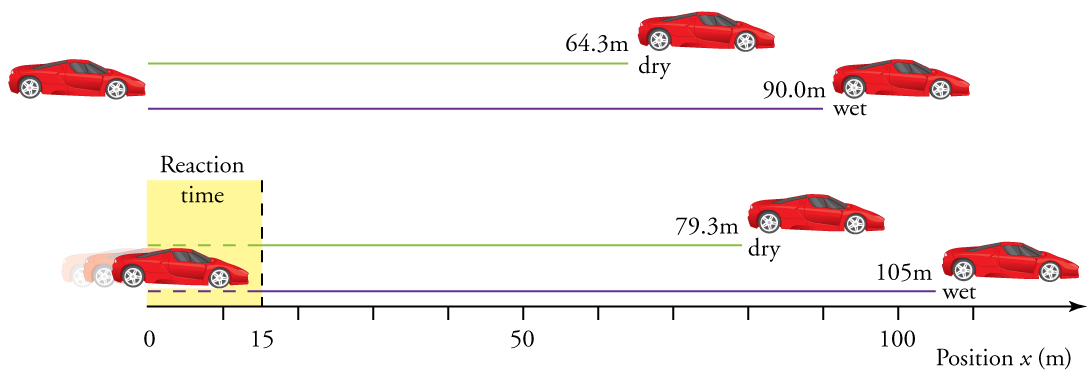
\includegraphics{images/Figure_02_04_03.jpg}
\caption{The distance necessary to stop a car varies greatly, depending on road
conditions and driver reaction time. Shown here are the braking
distances for dry and wet pavement, as calculated in this example, for a
car initially traveling at 30.0 m/s. Also shown are the total distances
traveled from the point where the driver first sees a light turn red,
assuming a 0.500 s reaction
time.}\label{import-auto-id1658840}
}
\end{figure}

\begin{tinysection}

{Discussion}

\end{tinysection}

The displacements found in this example seem reasonable for stopping a
fast-moving car. It should take longer to stop a car on wet rather than
dry pavement. It is interesting that reaction time adds significantly to
the displacements. But more important is the general approach to solving
problems. We identify the knowns and the quantities to be determined and
then find an appropriate equation. There is often more than one way to
solve a problem. The various parts of this example can in fact be solved
by other methods, but the solutions presented above are the shortest.

\hypertarget{fs-id1164906470852}{}
Calculating Time: A Car Merges into Traffic

Suppose a car merges into freeway traffic on a 200-m-long ramp. If its
initial velocity is 10.0 m/s and it accelerates at
\({2\text{.}\text{00\ m/s}^{2}}{}\), how long does it take to travel the
200 m up the ramp? (Such information might be useful to a traffic
engineer.)

\begin{tinysection}

{Strategy}

\end{tinysection}

Draw a sketch.

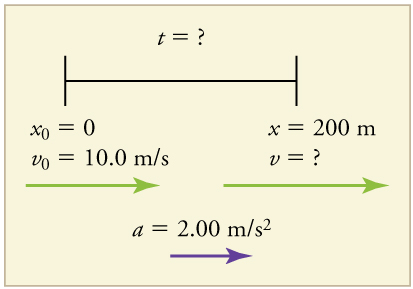
\includegraphics{images/Figure_02_04_03a.jpg}

We are asked to solve for the time \(t{}\). As before, we identify the
known quantities in order to choose a convenient physical relationship
(that is, an equation with one unknown, \(t{}\)).

\begin{tinysection}

{Solution}

\end{tinysection}

1. Identify the knowns and what we want to solve for. We know that
\({v_{0} = \text{10\ m/s}}{}\); \({{a = 2}\text{.}\text{00\ m/s}^{2}}{}\);
and \({x = \text{200\ m}}{}\).

2. We need to solve for \(t{}\). Choose the best equation.
\({{x = {x_{0} + v_{0}}}{t + \frac{1}{2}}\text{at}^{2}}{}\) works best
because the only unknown in the equation is the variable \(t{}\) for which
we need to solve.

3. We will need to rearrange the equation to solve for \(t{}\). In this
case, it will be easier to plug in the knowns first.

\leavevmode\hypertarget{import-auto-id2179013}{}%
\[{{\text{200\ m} = {\text{0\ m} + \left( {\text{10}\text{.}\text{0\ m/s}} \right)}}{t + \frac{1}{2}}\left( {2\text{.}\text{00\ m/s}^{2}} \right)\, t^{2}}{}\]

4. Simplify the equation. The units of meters (m) cancel because they
are in each term. We can get the units of seconds (s) to cancel by
taking \({{t = t}\ \text{s}}{}\), where \(t{}\) is the magnitude of time and
s is the unit. Doing so leaves

\leavevmode\hypertarget{eip-635}{}%
\[{{{\text{200} = \text{10}}{t + t^{2}}}\text{.}}{}\]

5. Use the quadratic formula to solve for \(t{}\)\emph{.}

\(a\) Rearrange the equation to get 0 on one side of the equation.

\leavevmode\hypertarget{import-auto-id1680208}{}%
\[{{t^{2} + \text{10}}{{t - \text{200}} = 0}}{}\]

This is a quadratic equation of the form

\leavevmode\hypertarget{import-auto-id1680214}{}%
\[{{{{\text{at}^{2} + \text{bt}} + c} = 0},}{}\]

where the constants are
\({{a = 1}\text{.}\text{00,}\ {b = \text{10}}\text{.}\text{0,}\ \text{and}\ {c = {- \text{200}}}}{}\).

\(b\) Its solutions are given by the quadratic formula:

\leavevmode\hypertarget{import-auto-id2367246}{}%
\[{t = \frac{{- b} \pm \sqrt{{b^{2} - 4}\text{ac}}}{2a}}\text{.}\]

This yields two solutions for \(t{}\), which are

\leavevmode\hypertarget{import-auto-id1772100}{}%
\[{{{t = \text{10}}\text{.}0\ \text{and}{- \text{20}}\text{.}0}.}{}\]

In this case, then, the time is
\({t = t}{}\)\emph{}
in\emph{} seconds, or

\leavevmode\hypertarget{import-auto-id2175275}{}%
\[{{{t = \text{10}}\text{.}0\ \text{s}\ {\text{and} - \text{20}}\text{.}0\ \text{s}}.}{}\]

A negative value for time is unreasonable, since it would mean that the
event happened 20 s before the motion began. We can discard that
solution. Thus,

\leavevmode\hypertarget{import-auto-id2177316}{}%
\[{{{t = \text{10}}\text{.}0\ \text{s}}.}{}\]

\begin{tinysection}

{Discussion}

\end{tinysection}

Whenever an equation contains an unknown squared, there will be two
solutions. In some problems both solutions are meaningful, but in
others, such as the above, only one solution is reasonable. The 10.0 s
answer seems reasonable for a typical freeway on-ramp.

With the basics of kinematics established, we can go on to many other
interesting examples and applications. In the process of developing
kinematics, we have also glimpsed a general approach to problem solving
that produces both correct answers and insights into physical
relationships. \href{/m54774}{Problem-Solving Basics} discusses
problem-solving basics and outlines an approach that will help you
succeed in this invaluable task.

\hypertarget{fs-id1164906508057}{}
\begin{note}

Making Connections: Take-Home Experiment---Breaking News

We have been using SI units of meters per second squared to describe
some examples of acceleration or deceleration of cars, runners, and
trains. To achieve a better feel for these numbers, one can measure the
braking deceleration of a car doing a slow (and safe) stop. Recall that,
for average acceleration, \({\overset{-}{a} = {\Delta v/\Delta t}}{}\).
While traveling in a car, slowly apply the brakes as you come up to a
stop sign. Have a passenger note the initial speed in miles per hour and
the time taken (in seconds) to stop. From this, calculate the
deceleration in miles per hour per second. Convert this to meters per
second squared and compare with other decelerations mentioned in this
chapter. Calculate the distance traveled in braking.

\end{note}

\hypertarget{fs-id1164906434690}{}
Check Your Understanding

\leavevmode\hypertarget{fs-id1164906434693}{}%
A manned rocket accelerates at a rate of \(\text{20\ m/s}^{2}{}\) during
launch. How long does it take the rocket reach a velocity of 400 m/s?

\leavevmode\hypertarget{fs-id1164906458555}{}%
To answer this, choose an equation that allows you to solve for time
\emph{\(t{}\)}, given only \(a{}\), \(v_{0}{}\), and \(v{}\).

\leavevmode\hypertarget{import-auto-id2168910}{}%
\[{v\, = \, v_{0} + \text{at}}{}\]

Rearrange to solve for \(t{}\)\emph{.}

\leavevmode\hypertarget{import-auto-id2168930}{}%
{t = v − v 0 a = 400 m/s − 0 m/s 20 m/s 2 = 20 s t = v − v 0 a = 400
m/s − 0 m/s 20 m/s 2 = 20 s size 12\{t= \{ \{v - v"" lSub \{ size 8\{0\} \} \}
over \{a\} \} = \{ \{"400 m/s" - "0 m/s"\} over \{"20 m/s" rSup \{ size
8\{2\} \} \} \} ="20 s"\} \{\}}

\hypertarget{fs-id1164906426121-summary}{}
\hypertarget{section-summary-4}{%
\subsection{Section Summary}\label{section-summary-4}}

\begin{itemize}
\item
  \protect\hypertarget{import-auto-id2171459}{}{To simplify calculations we take acceleration to be constant, so
  that \({\overset{-}{a} = a}{}\) at all times.}
\item
  \protect\hypertarget{import-auto-id2168260}{}{We also take initial time to be zero.}
\item
  \protect\hypertarget{import-auto-id2167408}{}{Initial position and velocity are given a subscript 0; final values
  have no subscript. Thus,}
  ::: \{\#import-auto-id2168257 data-type=``equation''\}
  \[\left. \begin{array}{lll}
  {\Delta t} & = & t \\
  {\Delta x} & = & {x - x_{0}} \\
  {\Delta v} & = & {v - v_{0}} \\
  \end{array} \right\}\]

  :::
\item
  \protect\hypertarget{import-auto-id2175179}{}{The following kinematic equations for motion with constant \(a{}\)
  are useful:}
  ::: \{\#import-auto-id2175197 data-type=``equation''\}
  \[{{x = {x_{0} + \overset{-}{v}}}t}{}\]

  :::

  \leavevmode\hypertarget{import-auto-id2175206}{}%
  \[{\overset{-}{v} = \frac{v_{0} + v}{2}}{}\]

  \leavevmode\hypertarget{import-auto-id2175249}{}%
  \[{v = {v_{0} + \text{at}}}{}\]

  \leavevmode\hypertarget{import-auto-id2176087}{}%
  \[{{x = {x_{0} + v_{0}}}{t + \frac{1}{2}}\text{at}^{2}}{}\]

  \leavevmode\hypertarget{import-auto-id2175231}{}%
  \[{{v^{2} = {v_{0}^{2} + 2a}}\left( {x - x_{0}} \right)}{}\]
\item
  \protect\hypertarget{import-auto-id2176131}{}{In vertical motion, \(y{}\) is substituted for
  \(x{}\).}
\end{itemize}

\hypertarget{fs-id1164906440394}{}
\begin{problems-exercises}

\hypertarget{problems-exercises-3}{%
\subsection{Problems \& Exercises}\label{problems-exercises-3}}

\hypertarget{fs-id1164906440403}{}
\leavevmode\hypertarget{fs-id1164906435871}{}%
An Olympic-class sprinter starts a race with an acceleration of
\({4\text{.}\text{50\ m/s}^{2}}{}\). (a) What is her speed 2.40 s later?
(b) Sketch a graph of her position vs.~time for this period.

\leavevmode\hypertarget{fs-id1164906440054}{}%
\(a\) \({\text{10}\text{.}8\ \text{m/s}}{}\)

\(b\)

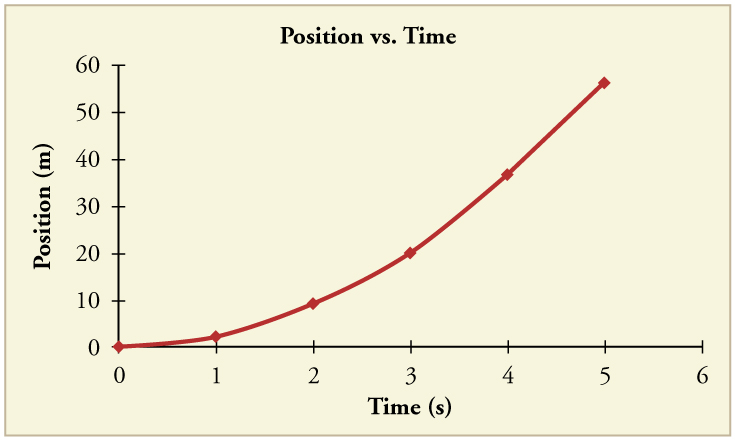
\includegraphics{images/unnumbered_art_p44.jpg}

\hypertarget{fs-id1164906478917}{}
\leavevmode\hypertarget{fs-id1164906478920}{}%
A well-thrown ball is caught in a well-padded mitt. If the deceleration
of the ball is
\({2\text{.}\text{10} \times \text{10}^{4}\ \text{m/s}^{2}}{}\), and 1.85
ms \({({\text{1\ ms} = \text{10}^{- 3}}\ \text{s})}{}\) elapses from the
time the ball first touches the mitt until it stops, what was the
initial velocity of the ball?

\leavevmode\hypertarget{fs-id1164906499124}{}%
38.9 m/s (about 87 miles per hour)

\hypertarget{fs-id1164906452216}{}
\leavevmode\hypertarget{fs-id1164906452219}{}%
A bullet in a gun is accelerated from the firing chamber to the end of
the barrel at an average rate of
\({6\text{.20} \times \text{10}^{5}\ \text{m/s}^{2}}{}\) for
\({8\text{.}\text{10} \times \text{10}^{- 4}\ \text{s}}{}\). What is its
muzzle velocity (that is, its final velocity)?

\hypertarget{fs-id1164906424347}{}
\leavevmode\hypertarget{fs-id1164906424350}{}%
\(a\) A light-rail commuter train accelerates at a rate of
\({1\text{.}\text{35\ m/s}^{2}}{}\). How long does it take to reach its
top speed of 80.0 km/h, starting from rest? (b) The same train
ordinarily decelerates at a rate of \({1\text{.}\text{65\ m/s}^{2}}{}\).
How long does it take to come to a stop from its top speed? (c) In
emergencies the train can decelerate more rapidly, coming to rest from
80.0 km/h in 8.30 s. What is its emergency deceleration in
\(\text{m/s}^{2}{}\)?

\leavevmode\hypertarget{fs-id1164906496443}{}%
\(a\) \({\text{16}\text{.}\text{5\ s}}{}\)

\(b\) \({\text{13}\text{.}\text{5\ s}}{}\)

\(c\) \({{- 2}\text{.}\text{68\ m/s}^{2}}{}\)

\hypertarget{fs-id1164906441407}{}
\leavevmode\hypertarget{fs-id1164906441410}{}%
While entering a freeway, a car accelerates from rest at a rate of
\({2\text{.}\text{40\ m/s}^{2}}{}\) for 12.0 s. (a) Draw a sketch of the
situation. (b) List the knowns in this problem. (c) How far does the car
travel in those 12.0 s? To solve this part, first identify the unknown,
and then discuss how you chose the appropriate equation to solve for it.
After choosing the equation, show your steps in solving for the unknown,
check your units, and discuss whether the answer is reasonable. (d) What
is the car's final velocity? Solve for this unknown in the same manner
as in part (c), showing all steps explicitly.

\hypertarget{fs-id1164906459799}{}
\leavevmode\hypertarget{fs-id1164906444281}{}%
At the end of a race, a runner decelerates from a velocity of 9.00 m/s
at a rate of \({2\text{.}\text{00\ m/s}^{2}}{}\). (a) How far does she
travel in the next 5.00 s? (b) What is her final velocity? (c) Evaluate
the result. Does it make sense?

\leavevmode\hypertarget{fs-id1164906453162}{}%
\(a\) \({\text{20}\text{.}\text{0\ m}}{}\)

\(b\) \({{- 1}\text{.}\text{00\ m/s}}{}\)

\(c\) This result does not really make sense. If the runner starts at
9.00 m/s and decelerates at \({2\text{.}\text{00\ m/s}^{2}}{}\), then she
will have stopped after 4.50 s. If she continues to decelerate, she will
be running backwards.

\hypertarget{fs-id1164906435065}{}
\hypertarget{fs-id1164906435068}{}
\begin{tinysection}

{Professional Application:}

\end{tinysection}

Blood is accelerated from rest to 30.0 cm/s in a distance of 1.80 cm by
the left ventricle of the heart. (a) Make a sketch of the situation. (b)
List the knowns in this problem. (c) How long does the acceleration
take? To solve this part, first identify the unknown, and then discuss
how you chose the appropriate equation to solve for it. After choosing
the equation, show your steps in solving for the unknown, checking your
units. (d) Is the answer reasonable when compared with the time for a
heartbeat?

\hypertarget{fs-id1164906467421}{}
\leavevmode\hypertarget{fs-id1164906467424}{}%
In a slap shot, a hockey player accelerates the puck from a velocity of
8.00 m/s to 40.0 m/s in the same direction. If this shot takes
\({3\text{.}\text{33} \times \text{10}^{- 2}\ \text{s}}{}\), calculate the
distance over which the puck accelerates.

\leavevmode\hypertarget{fs-id1164906461971}{}%
\({0\text{.}\text{799\ m}}{}\)

\hypertarget{fs-id1164906508513}{}
\leavevmode\hypertarget{fs-id1164906508516}{}%
A powerful motorcycle can accelerate from rest to 26.8 m/s (100 km/h) in
only 3.90 s. (a) What is its average acceleration? (b) How far does it
travel in that time?

\hypertarget{fs-id1164906451358}{}
\leavevmode\hypertarget{fs-id1164906451361}{}%
Freight trains can produce only relatively small accelerations and
decelerations. (a) What is the final velocity of a freight train that
accelerates at a rate of
\({0\text{.}\text{0500\ m/s}^{2}}{}\)\textsuperscript{} for
8.00 min, starting with an initial velocity of 4.00 m/s? (b) If the
train can slow down at a rate of \({0\text{.}\text{550\ m/s}^{2}}{}\), how
long will it take to come to a stop from this velocity? (c) How far will
it travel in each case?

\leavevmode\hypertarget{fs-id1164906495779}{}%
\(a\) \({\text{28}\text{.}\text{0\ m/s}}{}\)

\(b\) \({\text{50}\text{.}\text{9\ s}}{}\)

\(c\) 7.68 km to accelerate and 713 m to decelerate

\hypertarget{fs-id1164906430928}{}
\leavevmode\hypertarget{fs-id1164906430931}{}%
A fireworks shell is accelerated from rest to a velocity of 65.0 m/s
over a distance of 0.250 m. (a) How long did the acceleration last? (b)
Calculate the acceleration.

\hypertarget{fs-id1164906453058}{}
\leavevmode\hypertarget{fs-id1164906453061}{}%
A swan on a lake gets airborne by flapping its wings and running on top
of the water. (a) If the swan must reach a velocity of 6.00 m/s to take
off and it accelerates from rest at an average rate of
\({0\text{.}\text{350\ m/s}^{2}}{}\), how far will it travel before
becoming airborne? (b) How long does this take?

\leavevmode\hypertarget{fs-id1164906478379}{}%
\(a\) \({51\text{.}4\ \text{m}}{}\)

\(b\) \({\text{17}\text{.}\text{1\ s}}{}\)

\hypertarget{fs-id1164906459326}{}
\hypertarget{fs-id1164906459329}{}
\begin{tinysection}

{Professional Application:}

\end{tinysection}

A woodpecker's brain is specially protected from large decelerations by
tendon-like attachments inside the skull. While pecking on a tree, the
woodpecker's head comes to a stop from an initial velocity of 0.600 m/s
in a distance of only 2.00 mm. (a) Find the acceleration in
\(\text{m/s}^{2}{}\)\textsuperscript{} and in multiples of
\({g\ \left( {{g = 9}\text{.}\text{80}\ \text{m/s}^{2}} \right)}{}\). (b)
Calculate the stopping time. (c) The tendons cradling the brain stretch,
making its stopping distance 4.50 mm (greater than the head and, hence,
less deceleration of the brain). What is the brain's deceleration,
expressed in multiples of \(g\)?

\hypertarget{fs-id1164906466373}{}
\leavevmode\hypertarget{fs-id1164906466376}{}%
An unwary football player collides with a padded goalpost while running
at a velocity of 7.50 m/s and comes to a full stop after compressing the
padding and his body 0.350 m. (a) What is his deceleration? (b) How long
does the collision last?

\leavevmode\hypertarget{fs-id1164906466801}{}%
\(a\) \({{- \text{80}}\text{.}4\ \text{m/s}^{2}}{}\)

\(b\) \({9\text{.}{\text{33} \times \text{10}^{- 2}\ }\text{s}}{}\)

\hypertarget{fs-id1164906495926}{}
\leavevmode\hypertarget{fs-id1164906495929}{}%
In World War II, there were several reported cases of airmen who jumped
from their flaming airplanes with no parachute to escape certain death.
Some fell about 20,000 feet (6000 m), and some of them survived, with
few life-threatening injuries. For these lucky pilots, the tree branches
and snow drifts on the ground allowed their deceleration to be
relatively small. If we assume that a pilot's speed upon impact was 123
mph (54 m/s), then what was his deceleration? Assume that the trees and
snow stopped him over a distance of 3.0 m.

\hypertarget{fs-id1164906495944}{}
\leavevmode\hypertarget{fs-id1164906495948}{}%
Consider a grey squirrel falling out of a tree to the ground. (a) If we
ignore air resistance in this case (only for the sake of this problem),
determine a squirrel's velocity just before hitting the ground,
assuming it fell from a height of 3.0 m. (b) If the squirrel stops in a
distance of 2.0 cm through bending its limbs, compare its deceleration
with that of the airman in the previous problem.

\leavevmode\hypertarget{fs-id1164906459010}{}%
\(a\) \({7\text{.}\text{7\ m/s}}{}\)

\(b\) \({{{- \text{15}} \times \text{10}^{2}}\ \text{m/s}^{2}}{}\). This
is about 3 times the deceleration of the pilots, who were falling from
thousands of meters high!

\hypertarget{fs-id1164906433746}{}
\leavevmode\hypertarget{fs-id1164906433747}{}%
An express train passes through a station. It enters with an initial
velocity of 22.0 m/s and decelerates at a rate of
\({0\text{.}\text{150\ m/s}^{2}}{}\) as it goes through. The station is
210 m long. (a) How long is the nose of the train in the station? (b)
How fast is it going when the nose leaves the station? (c) If the train
is 130 m long, when does the end of the train leave the station? (d)
What is the velocity of the end of the train as it leaves?

\hypertarget{fs-id1164906502756}{}
\leavevmode\hypertarget{fs-id1164906502757}{}%
Dragsters can actually reach a top speed of 145 m/s in only 4.45
s---considerably less time than given in
\protect\hyperlink{fs-id1164906457202}{link} and
\protect\hyperlink{fs-id1164906443776}{link}. (a) Calculate the
average acceleration for such a dragster. (b) Find the final velocity of
this dragster starting from rest and accelerating at the rate found in
(a) for 402 m (a quarter mile) without using any information on time.
(c) Why is the final velocity greater than that used to find the average
acceleration? \emph{Hint}: Consider whether the assumption of constant
acceleration is valid for a dragster. If not, discuss whether the
acceleration would be greater at the beginning or end of the run and
what effect that would have on the final velocity.

\leavevmode\hypertarget{fs-id1164906446759}{}%
\(a\) \({\text{32}\text{.}\text{6\ m/s}^{2}}{}\)

\(b\) \(\text{162\ m/s}{}\)

\(c\) \({v > v_{\text{max}}}{}\), because the assumption of constant
acceleration is not valid for a dragster. A dragster changes gears, and
would have a greater acceleration in first gear than second gear than
third gear, etc. The acceleration would be greatest at the beginning, so
it would not be accelerating at \({\text{32}\text{.}\text{6\ m/s}^{2}}{}\)
during the last few meters, but substantially less, and the final
velocity would be less than 162 m/s.

\hypertarget{fs-id1164906479070}{}
\leavevmode\hypertarget{fs-id1164906479073}{}%
A bicycle racer sprints at the end of a race to clinch a victory. The
racer has an initial velocity of 11.5 m/s and accelerates at the rate of
\({0\text{.}\text{500\ m/s}^{2}}{}\) for 7.00 s. (a) What is his final
velocity? (b) The racer continues at this velocity to the finish line.
If he was 300 m from the finish line when he started to accelerate, how
much time did he save? (c) One other racer was 5.00 m ahead when the
winner started to accelerate, but he was unable to accelerate, and
traveled at 11.8 m/s until the finish line. How far ahead of him (in
meters and in seconds) did the winner finish?

\hypertarget{fs-id1164906433774}{}
\leavevmode\hypertarget{fs-id1164906433777}{}%
In 1967, New Zealander Burt Munro set the world record for an Indian
motorcycle, on the Bonneville Salt Flats in Utah, with a maximum speed
of 183.58 mi/h. The one-way course was 5.00 mi long. Acceleration rates
are often described by the time it takes to reach 60.0 mi/h from rest.
If this time was 4.00 s, and Burt accelerated at this rate until he
reached his maximum speed, how long did it take Burt to complete the
course?

\leavevmode\hypertarget{fs-id1164906433797}{}%
104 s

\hypertarget{fs-id1164906508150}{}
\leavevmode\hypertarget{fs-id1164906508153}{}%
\(a\) A world record was set for the men's 100-m dash in the 2008
Olympic Games in Beijing by Usain Bolt of Jamaica. Bolt ``coasted'' across
the finish line with a time of 9.69 s. If we assume that Bolt
accelerated for 3.00 s to reach his maximum speed, and maintained that
speed for the rest of the race, calculate his maximum speed and his
acceleration. (b) During the same Olympics, Bolt also set the world
record in the 200-m dash with a time of 19.30 s. Using the same
assumptions as for the 100-m dash, what was his maximum speed for this
race?

\leavevmode\hypertarget{fs-id1164906508162}{}%
\(a\) \({{v = \text{12}}\text{.}\text{2\ m/s}}{}\);
\({{a = 4}\text{.}\text{07\ m/s}^{2}}{}\)

\(b\) \({{v = \text{11}}\text{.}\text{2\ m/s}}{}\)

\end{problems-exercises}

\hypertarget{fs-id2388866}{}
\begin{ap-test-prep}

\hypertarget{test-prep-for-ap-courses-4}{%
\subsection{Test Prep for AP Courses}\label{test-prep-for-ap-courses-4}}

\hypertarget{fs-id1844508}{}
\leavevmode\hypertarget{fs-id1844512}{}%
A group of students is attempting to determine the average acceleration
of a marble released from the top of a long ramp. Below is a set of data
representing the marble's position with respect to time.

\begin{longtable}[]{@{}ll@{}}
\toprule
Position (cm) & Time (s)\tabularnewline
\midrule
\endhead
0.0 & 0.0\tabularnewline
0.3 & 0.5\tabularnewline
1.25 & 1.0\tabularnewline
2.8 & 1.5\tabularnewline
5.0 & 2.0\tabularnewline
7.75 & 2.5\tabularnewline
11.3 & 3.0\tabularnewline
\bottomrule
\end{longtable}

Use the data table above to construct a graph determining the
acceleration of the marble. Select a set of data points from the table
and plot those points on the graph. Fill in the blank column in the
table for any quantities you graph other than the given data. Label the
axes and indicate the scale for each. Draw a best-fit line or curve
through your data points.

Using the best-fit line, determine the value of the marble's
acceleration.

\end{ap-test-prep}

\hypertarget{problem-solving-basics-for-one-dimensional-kinematics}{%
\section{Problem-Solving Basics for One Dimensional Kinematics}\label{problem-solving-basics-for-one-dimensional-kinematics}}

\begin{figure}
\hypertarget{import-auto-id1788945}{%
\centering
\includegraphics{images/Figure_02_06_00.jpg}
\caption{Problem-solving skills are essential to your success in Physics.
(credit: scui3asteveo,
Flickr)}\label{import-auto-id1788945}
}
\end{figure}

\hypertarget{fs-id2494789}{}
\begin{learning-objectives}

\hypertarget{learning-objectives-4}{%
\subsection{Learning Objectives}\label{learning-objectives-4}}

By the end of this section, you will be able to:

\begin{itemize}
\tightlist
\item
  Apply problem-solving steps and strategies to solve problems of
  one-dimensional kinematics.
\item
  Apply strategies to determine whether or not the result of a problem
  is reasonable, and if not, determine the cause.
\end{itemize}

\end{learning-objectives}

Problem-solving skills are obviously essential to success in a
quantitative course in physics. More importantly, the ability to apply
broad physical principles, usually represented by equations, to specific
situations is a very powerful form of knowledge. It is much more
powerful than memorizing a list of facts. Analytical skills and
problem-solving abilities can be applied to new situations, whereas a
list of facts cannot be made long enough to contain every possible
circumstance. Such analytical skills are useful both for solving
problems in this text and for applying physics in everyday and
professional life.

\hypertarget{fs-id952201}{}
\hypertarget{problem-solving-steps}{%
\subsection{Problem-Solving Steps}\label{problem-solving-steps}}

While there is no simple step-by-step method that works for every
problem, the following general procedures facilitate problem solving and
make it more meaningful. A certain amount of creativity and insight is
required as well.

\hypertarget{fs-id2092387}{}
\hypertarget{step-1}{%
\subsubsection{Step 1}\label{step-1}}

\emph{Examine the situation to determine which physical principles are
involved}. It often helps to \emph{draw a simple sketch} at the outset. You
will also need to decide which direction is positive and note that on
your sketch. Once you have identified the physical principles, it is
much easier to find and apply the equations representing those
principles. Although finding the correct equation is essential, keep in
mind that equations represent physical principles, laws of nature, and
relationships among physical quantities. Without a conceptual
understanding of a problem, a numerical solution is meaningless.

\hypertarget{fs-id2204794}{}
\hypertarget{step-2}{%
\subsubsection{Step 2}\label{step-2}}

\emph{Make a list of what is given or can be inferred from the problem as
stated (identify the knowns)}. Many problems are stated very succinctly
and require some inspection to determine what is known. A sketch can
also be very useful at this point. Formally identifying the knowns is of
particular importance in applying physics to real-world situations.
Remember, ``stopped'' means velocity is zero, and we often can take
initial time and position as zero.

\hypertarget{fs-id1754393}{}
\hypertarget{step-3}{%
\subsubsection{Step 3}\label{step-3}}

\emph{Identify exactly what needs to be determined in the problem (identify
the unknowns)}. In complex problems, especially, it is not always
obvious what needs to be found or in what sequence. Making a list can
help.

\hypertarget{fs-id758749}{}
\hypertarget{step-4}{%
\subsubsection{Step 4}\label{step-4}}

\emph{Find an equation or set of equations that can help you solve the
problem}. Your list of knowns and unknowns can help here. It is easiest
if you can find equations that contain only one unknown---that is, all
of the other variables are known, so you can easily solve for the
unknown. If the equation contains more than one unknown, then an
additional equation is needed to solve the problem. In some problems,
several unknowns must be determined to get at the one needed most. In
such problems it is especially important to keep physical principles in
mind to avoid going astray in a sea of equations. You may have to use
two (or more) different equations to get the final answer.

\hypertarget{fs-id1770068}{}
\hypertarget{step-5}{%
\subsubsection{Step 5}\label{step-5}}

\emph{Substitute the knowns along with their units into the appropriate
equation, and obtain numerical solutions complete with units}. This step
produces the numerical answer; it also provides a check on units that
can help you find errors. If the units of the answer are incorrect, then
an error has been made. However, be warned that correct units do not
guarantee that the numerical part of the answer is also correct.

\hypertarget{fs-id1372026}{}
\hypertarget{step-6}{%
\subsubsection{Step 6}\label{step-6}}

\emph{Check the answer to see if it is reasonable: Does it make sense?} This
final step is extremely important---the goal of physics is to accurately
describe nature. To see if the answer is reasonable, check both its
magnitude and its sign, in addition to its units. Your judgment will
improve as you solve more and more physics problems, and it will become
possible for you to make finer and finer judgments regarding whether
nature is adequately described by the answer to a problem. This step
brings the problem back to its conceptual meaning. If you can judge
whether the answer is reasonable, you have a deeper understanding of
physics than just being able to mechanically solve a problem.

When solving problems, we often perform these steps in different order,
and we also tend to do several steps simultaneously. There is no rigid
procedure that will work every time. Creativity and insight grow with
experience, and the basics of problem solving become almost automatic.
One way to get practice is to work out the text's examples for yourself
as you read. Another is to work as many end-of-section problems as
possible, starting with the easiest to build confidence and progressing
to the more difficult. Once you become involved in physics, you will see
it all around you, and you can begin to apply it to situations you
encounter outside the classroom, just as is done in many of the
applications in this text.

\hypertarget{fs-id2176647}{}
\hypertarget{unreasonable-results}{%
\subsection{Unreasonable Results}\label{unreasonable-results}}

Physics must describe nature accurately. Some problems have results that
are unreasonable because one premise is unreasonable or because certain
premises are inconsistent with one another. The physical principle
applied correctly then produces an unreasonable result. For example, if
a person starting a foot race accelerates at
\({0\text{.}\text{40\ m/s}^{2}}{}\) for 100 s, his final speed will be 40
m/s (about 150 km/h)---clearly unreasonable because the time of 100 s is
an unreasonable premise. The physics is correct in a sense, but there is
more to describing nature than just manipulating equations correctly.
Checking the result of a problem to see if it is reasonable does more
than help uncover errors in problem solving---it also builds intuition
in judging whether nature is being accurately described.

Use the following strategies to determine whether an answer is
reasonable and, if it is not, to determine what is the cause.

\hypertarget{fs-id1987367}{}
\hypertarget{step-1-1}{%
\subsubsection{Step 1}\label{step-1-1}}

\emph{Solve the problem using strategies as outlined and in the format
followed in the worked examples in the text}. In the example given in
the preceding paragraph, you would identify the givens as the
acceleration and time and use the equation below to find the unknown
final velocity. That is,

\leavevmode\hypertarget{import-auto-id4167672}{}%
\[{{{{v = {v_{0} + \text{at}}} = {0 + \left( {0\text{.}\text{40}\ \text{m/s}^{2}} \right)}}{\left( {\text{100}\ \text{s}} \right) = \text{40}}\ \text{m/s}}.}{}\]

\hypertarget{fs-id2525779}{}
\hypertarget{step-2-1}{%
\subsubsection{Step 2}\label{step-2-1}}

\emph{Check to see if the answer is reasonable}. Is it too large or too
small, or does it have the wrong sign, improper units, \ldots? In this
case, you may need to convert meters per second into a more familiar
unit, such as miles per hour.

\leavevmode\hypertarget{import-auto-id1437508}{}%
\[\left( \frac{\text{40\ m}}{s} \right)\left( \frac{\text{3.28\ ft}}{m} \right)\left( \frac{\text{1\ mi}}{\text{5280\ ft}} \right)\left( \frac{\text{60\ s}}{\text{min}} \right){\left( \frac{\text{60\ min}}{\text{1\ h}} \right) = 89\ mph}\]

This velocity is about four times greater than a person can run---so it
is too large.

\hypertarget{fs-id4130945}{}
\hypertarget{step-3-1}{%
\subsubsection{Step 3}\label{step-3-1}}

\emph{If the answer is unreasonable, look for what specifically could cause
the identified difficulty}. In the example of the runner, there are only
two assumptions that are suspect. The acceleration could be too great or
the time too long. First look at the acceleration and think about what
the number means. If someone accelerates at
\({0\text{.}\text{40\ m/s}^{2}}{}\), their velocity is increasing by 0.4
m/s each second. Does this seem reasonable? If so, the time must be too
long. It is not possible for someone to accelerate at a constant rate of
\({0\text{.}\text{40\ m/s}^{2}}{}\) for 100 s (almost two minutes).

\hypertarget{fs-id1602384-summary}{}
\hypertarget{section-summary-5}{%
\subsection{Section Summary}\label{section-summary-5}}

\begin{itemize}
\item
  \protect\hypertarget{import-auto-id927917}{}{\emph{The six basic problem solving steps for physics
  are:}}

  \emph{Step 1}. Examine the situation to determine which physical
  principles are involved.

  \emph{Step 2}. Make a list of what is given or can be inferred from the
  problem as stated (identify the knowns).

  \emph{Step 3}. Identify exactly what needs to be determined in the
  problem (identify the unknowns).

  \emph{Step 4}. Find an equation or set of equations that can help you
  solve the problem.

  \emph{Step 5}. Substitute the knowns along with their units into the
  appropriate equation, and obtain numerical solutions complete with
  units.

  \emph{Step 6}. Check the answer to see if it is reasonable: Does it make
  sense?
\end{itemize}

\hypertarget{fs-id2577484}{}
\begin{conceptual-questions}

\hypertarget{conceptual-questions-4}{%
\subsection{Conceptual Questions}\label{conceptual-questions-4}}

\hypertarget{fs-id4087579}{}
\leavevmode\hypertarget{fs-id4067228}{}%
What information do you need in order to choose which equation or
equations to use to solve a problem? Explain.

\hypertarget{fs-id1986766}{}
\leavevmode\hypertarget{fs-id2013359}{}%
What is the last thing you should do when solving a problem? Explain.

\end{conceptual-questions}

\hypertarget{falling-objects}{%
\section{Falling Objects}\label{falling-objects}}

\hypertarget{fs-id3275688}{}
\begin{learning-objectives}

\hypertarget{learning-objectives-5}{%
\subsection{Learning Objectives}\label{learning-objectives-5}}

By the end of this section, you will be able to:

\begin{itemize}
\tightlist
\item
  Describe the effects of gravity on objects in motion.
\item
  Describe the motion of objects that are in free fall.
\item
  Calculate the position and velocity of objects in free fall.
\end{itemize}

The information presented in this section supports the following AP®
learning objectives and science practices:

\begin{itemize}
\tightlist
\item
  \textbf{3.A.1.1} The student is able to express the motion of an object
  using narrative, mathematical, or graphical representations. \textbf{(S.P.
  1.5, 2.1, 2.2)}
\item
  \textbf{3.A.1.2} The student is able to design an experimental
  investigation of the motion of an object. \textbf{(S.P. 4.2)}
\item
  \textbf{3.A.1.3} The student is able to analyze experimental data
  describing the motion of an object and is able to express the
  results of the analysis using narrative, mathematical, and graphical
  representations. \textbf{(S.P. 5.1)}
\end{itemize}

\end{learning-objectives}

Falling objects form an interesting class of motion problems. For
example, we can estimate the depth of a vertical mine shaft by dropping
a rock into it and listening for the rock to hit the bottom. By applying
the kinematics developed so far to falling objects, we can examine some
interesting situations and learn much about gravity in the process.

\hypertarget{fs-id4178141}{}
\hypertarget{gravity}{%
\subsection{Gravity}\label{gravity}}

The most remarkable and unexpected fact about falling objects is that,
if air resistance and friction are negligible, then in a given location
all objects fall toward the center of Earth with the \emph{same constant
acceleration}, \emph{independent of their mass}. This experimentally
determined fact is unexpected, because we are so accustomed to the
effects of air resistance and friction that we expect light objects to
fall slower than heavy ones.

\begin{figure}
\hypertarget{import-auto-id4126662}{%
\centering
\includegraphics{images/Figure_02_07_00a.jpg}
\caption{A hammer and a feather will fall with the same constant acceleration
if air resistance is considered negligible. This is a general
characteristic of gravity not unique to Earth, as astronaut David R.
Scott demonstrated on the Moon in 1971, where the acceleration due to
gravity is only
\({1\text{.}\text{67\ m/s}^{2}}{}\).}\label{import-auto-id4126662}
}
\end{figure}

In the real world, air resistance can cause a lighter object to fall
slower than a heavier object of the same size. A tennis ball will reach
the ground after a hard baseball dropped at the same time. (It might be
difficult to observe the difference if the height is not large.) Air
resistance opposes the motion of an object through the air, while
friction between objects---such as between clothes and a laundry chute
or between a stone and a pool into which it is dropped---also opposes
motion between them. For the ideal situations of these first few
chapters, an object \emph{falling without air resistance or friction} is
defined to be in \protect\hypertarget{import-auto-id1714641}{}{free-fall}.

The force of gravity causes objects to fall toward the center of Earth.
The acceleration of free-falling objects is therefore called the
\protect\hypertarget{import-auto-id1707599}{}{acceleration due to gravity}.
The acceleration due to gravity is \emph{constant}, which means we can apply
the kinematics equations to any falling object where air resistance and
friction are negligible. This opens a broad class of interesting
situations to us. The acceleration due to gravity is so important that
its magnitude is given its own symbol, \(g{}\). It is constant at any
given location on Earth and has the average value

\leavevmode\hypertarget{eip-636}{}%
\[{{g = 9}\text{.}\text{80\ m/s}^{2}}\text{.}{}\]

Although \(g{}\) varies from \({9\text{.}\text{78\ m/s}^{2}}{}\) to
\({9\text{.}\text{83\ m/s}^{2}}{}\), depending on latitude, altitude,
underlying geological formations, and local topography, the average
value of \({9\text{.}\text{80\ m/s}^{2}}{}\) will be used in this text
unless otherwise specified. The direction of the acceleration due to
gravity is \emph{downward (towards the center of Earth)}. In fact, its
direction \emph{defines} what we call vertical. Note that whether the
acceleration \(a{}\) in the kinematic equations has the value \({+ g}{}\) or
\({- g}{}\) depends on how we define our coordinate system. If we define
the upward direction as positive, then
\({{{a = {- g}} = {- 9}}\text{.}\text{80\ m/s}^{2}}{}\), and if we define
the downward direction as positive, then
\({{{a = g} = 9}\text{.}\text{80\ m/s}^{2}}{}\).

\hypertarget{fs-id2854808}{}
\hypertarget{one-dimensional-motion-involving-gravity}{%
\subsection{One-Dimensional Motion Involving Gravity}\label{one-dimensional-motion-involving-gravity}}

The best way to see the basic features of motion involving gravity is to
start with the simplest situations and then progress toward more complex
ones. So we start by considering straight up and down motion with no air
resistance or friction. These assumptions mean that the velocity (if
there is any) is vertical. If the object is dropped, we know the initial
velocity is zero. Once the object has left contact with whatever held or
threw it, the object is in free-fall. Under these circumstances, the
motion is one-dimensional and has constant acceleration of magnitude
\(g{}\). We will also represent vertical displacement with the symbol
\(y{}\) and use \(x{}\) for horizontal displacement.

\hypertarget{fs-id1931991}{}
\begin{note}

Kinematic Equations for Objects in Free-Fall where Acceleration = -\emph{g}

\leavevmode\hypertarget{import-auto-id2222965}{}%
\[{v = {v_{0} - \text{gt}}}{}\]

\leavevmode\hypertarget{import-auto-id4048491}{}%
\[{{y = {y_{0} + v_{0}}}{t - \frac{1}{2}}\text{gt}^{2}}{}\]

\leavevmode\hypertarget{import-auto-id4019890}{}%
\[{{v^{2} = {v_{0}^{2} - 2g}}\left( {y - y_{0}} \right)}{}\]

\end{note}

\hypertarget{fs-id4067058}{}
Calculating Position and Velocity of a Falling Object: A Rock Thrown
Upward

A person standing on the edge of a high cliff throws a rock straight up
with an initial velocity of 13.0 m/s. The rock misses the edge of the
cliff as it falls back to Earth. Calculate the position and velocity of
the rock 1.00 s, 2.00 s, and 3.00 s after it is thrown, neglecting the
effects of air resistance.

\begin{tinysection}

{Strategy}

\end{tinysection}

Draw a sketch.

\includegraphics{images/Figure_02_07_00b.jpg}

We are asked to determine the position \(y{}\) at various times. It is
reasonable to take the initial position \(y_{0}{}\) to be zero. This
problem involves one-dimensional motion in the vertical direction. We
use plus and minus signs to indicate direction, with up being positive
and down negative. Since up is positive, and the rock is thrown upward,
the initial velocity must be positive too. The acceleration due to
gravity is downward, so \(a{}\) is negative. It is crucial that the
initial velocity and the acceleration due to gravity have opposite
signs. Opposite signs indicate that the acceleration due to gravity
opposes the initial motion and will slow and eventually reverse it.

Since we are asked for values of position and velocity at three times,
we will refer to these as \(y_{1}{}\) and \(v_{1}{}\); \emph{\(y_{2}{}\)} and
\(v_{2}{}\); and \(y_{3}{}\) and \(v_{3}{}\).

\textbf{Solution for Position} \(y_{1}{}\)

1. Identify the knowns. We know that \({y_{0} = 0}{}\);
\({{v_{0} = \text{13}}\text{.}\text{0\ m/s}}{}\);
\({{{a = {- g}} = {- 9}}\text{.}\text{80\ m/s}^{2}}{}\); and
\({{t = 1}\text{.}\text{00\ s}}{}\).

2. Identify the best equation to use. We will use
\({{y = {y_{0} + v_{0}}}{t + \frac{1}{2}}\text{at}^{2}}{}\) because it
includes only one unknown, \(y{}\) (or \(y_{1}{}\),
here),\emph{} which is the value we want to
find.

3. Plug in the known values and solve for \(y_{1}{}\).

\leavevmode\hypertarget{import-auto-id2302522}{}%
{y 1 = 0 + 13 . 0 m/s 1 . 00 s + 1 2 − 9 . 80 m/s 2 1 . 00 s 2 = 8 . 10
m y 1 = 0 + 13 . 0 m/s 1 . 00 s + 1 2 − 9 . 80 m/s 2 1 . 00 s 2 = 8 . 10
m size 12\{y"" lSub \{ size 8\{1\} \} =0+ left ("13" "." "0 m/s"
right ) left (1 "." "00 s" right )+ \{ \{1\} over \{2\} \} left ( - 9
"." "80"" m/s" rSup \{ size 8\{2\} \} right ) left (1 "." "00 s"
right ) rSup \{ size 8\{2\} \} =8 "." "10"`m\} \{\}}

\begin{tinysection}

{Discussion}

\end{tinysection}

The rock is 8.10 m above its starting point at
\({{t = 1}\text{.}\text{00}}{}\) s, since \({y_{1} > y_{0}}{}\). It could be
\emph{moving} up or down; the only way to tell is to calculate \(v_{1}{}\) and
find out if it is positive or negative.

\textbf{Solution for Velocity} \(v_{1}{}\)

1. Identify the knowns. We know that \({y_{0} = 0}{}\);
\({{v_{0} = \text{13}}\text{.}\text{0\ m/s}}{}\);
\({{{a = {- g}} = {- 9}}\text{.}\text{80\ m/s}^{2}}{}\); and
\({{t = 1}\text{.}\text{00\ s}}{}\). We also know from the solution above
that \({{y_{1} = 8}\text{.}\text{10\ m}}{}\).

2. Identify the best equation to use. The most straightforward is
\({v = {v_{0} - \text{gt}}}{}\) (from \({v = {v_{0} + \text{at}}}{}\), where
\({{a = \text{gravitational\ acceleration}} = {- g}}{}\)).

3. Plug in the knowns and solve.

\leavevmode\hypertarget{import-auto-id1688803}{}%
\[{{{v_{1} = {v_{0} - \text{gt}}} = \text{13}}\text{.}{\text{0\ m/s} - \left( {9\text{.}\text{80\ m/s}^{2}} \right)}{\left( {1\text{.}\text{00\ s}} \right) = 3}\text{.}\text{20\ m/s}}{}\]

\begin{tinysection}

{Discussion}

\end{tinysection}

The positive value for \(v_{1}{}\) means that the rock is still heading
upward at \({{t = 1}\text{.}\text{00}\ \text{s}}{}\). However, it has
slowed from its original 13.0\emph{} m/s, as
expected.

\textbf{Solution for Remaining Times}

The procedures for calculating the position and velocity at
\({{t = 2}\text{.}\text{00}\ \text{s}}{}\) and \({3\text{.}\text{00\ s}}{}\)
are the same as those above. The results are summarized in
\protect\hyperlink{eip-304}{link} and illustrated in
\protect\hyperlink{import-auto-id4064055}{link}.

\begin{longtable}[]{@{}llll@{}}
\caption{{Results}}\tabularnewline
\toprule
Time, \emph{t} & Position, \emph{y} & Velocity, \emph{v} & Acceleration, \emph{a}\tabularnewline
\midrule
\endfirsthead
\toprule
Time, \emph{t} & Position, \emph{y} & Velocity, \emph{v} & Acceleration, \emph{a}\tabularnewline
\midrule
\endhead
\({1\text{.}\text{00\ s}}{}\) & \({8\text{.}\text{10\ m}}{}\) & \({3\text{.}\text{20\ m/s}}{}\) & \({{- 9}\text{.}\text{80\ m/s}^{2}}{}\)\tabularnewline
\({2\text{.}\text{00\ s}}{}\) & \({6\text{.}\text{40\ m}}{}\) & \({{- 6}\text{.}\text{60\ m/s}}{}\) & \({{- 9}\text{.}\text{80\ m/s}^{2}}{}\)\tabularnewline
\({3\text{.}\text{00\ s}}{}\) & \({{- 5}\text{.}\text{10\ m}}{}\) & \({{- \text{16}}\text{.}\text{4\ m/s}}{}\) & \({{- 9}\text{.}\text{80\ m/s}^{2}}{}\)\tabularnewline
\bottomrule
\end{longtable}

Graphing the data helps us understand it more clearly.

\begin{figure}
\hypertarget{import-auto-id4064055}{%
\centering
\includegraphics{images/Figure_02_06_01.jpg}
\caption{Vertical position, vertical velocity, and vertical acceleration vs.
time for a rock thrown vertically up at the edge of a cliff. Notice that
velocity changes linearly with time and that acceleration is constant.
\emph{Misconception Alert!} Notice that the position vs.~time graph shows
vertical position only. It is easy to get the impression that the graph
shows some horizontal motion---the shape of the graph looks like the
path of a projectile. But this is not the case; the horizontal axis is
\emph{time}, not space. The actual path of the rock in space is straight up,
and straight down.}\label{import-auto-id4064055}
}
\end{figure}

\begin{tinysection}

{Discussion}

\end{tinysection}

The interpretation of these results is important. At 1.00 s the rock is
above its starting point and heading upward, since \(y_{1}{}\) and
\(v_{1}{}\) are both positive. At 2.00 s, the rock is still above its
starting point, but the negative velocity means it is moving downward.
At 3.00 s, both \(y_{3}{}\) and \(v_{3}{}\) are negative, meaning the rock
is below its starting point and continuing to move downward. Notice that
when the rock is at its highest point (at 1.5 s), its velocity is zero,
but its acceleration is still \({{- 9}\text{.}\text{80\ m/s}^{2}}{}\). Its
acceleration is
\({{- 9}\text{.}\text{80\ m/s}^{2}}{}\)\textsuperscript{}
for the whole trip---while it is moving up and while it is moving down.
Note that the values for \(y{}\)\emph{} are the
positions (or displacements) of the rock, not the total distances
traveled. Finally, note that free-fall applies to upward motion as well
as downward. Both have the same acceleration---the acceleration due to
gravity, which remains constant the entire time. Astronauts training in
the famous Vomit Comet, for example, experience free-fall while arcing
up as well as down, as we will discuss in more detail later.

\hypertarget{fs-id1773192}{}
\begin{note}

Making Connections: Take-Home Experiment---Reaction Time

A simple experiment can be done to determine your reaction time. Have a
friend hold a ruler between your thumb and index finger, separated by
about 1 cm. Note the mark on the ruler that is right between your
fingers. Have your friend drop the ruler unexpectedly, and try to catch
it between your two fingers. Note the new reading on the ruler. Assuming
acceleration is that due to gravity, calculate your reaction time. How
far would you travel in a car (moving at 30 m/s) if the time it took
your foot to go from the gas pedal to the brake was twice this reaction
time?

\end{note}

\hypertarget{fs-id2186600}{}
Calculating Velocity of a Falling Object: A Rock Thrown Down

What happens if the person on the cliff throws the rock straight down,
instead of straight up? To explore this question, calculate the velocity
of the rock when it is 5.10 m below the starting point, and has been
thrown downward with an initial speed of 13.0 m/s.

\begin{tinysection}

{Strategy}

\end{tinysection}

Draw a sketch.

\includegraphics{images/Figure_02_06_01a.jpg}

Since up is positive, the final position of the rock will be negative
because it finishes below the starting point at \({y_{0} = 0}{}\).
Similarly, the initial velocity is downward and therefore negative, as
is the acceleration due to gravity. We expect the final velocity to be
negative since the rock will continue to move downward.

\begin{tinysection}

{Solution}

\end{tinysection}

1. Identify the knowns. \(y_{0} = 0\);
\({y_{1}{= - 5}}\text{.}\text{10\ m}\);
\(v_{0} = {- \text{13}}\text{.0\ m/s}\);
\({{{a = {- g}} = {- 9}}\text{.}\text{80\ m}\text{/s}^{2}}{}\).

2. Choose the kinematic equation that makes it easiest to solve the
problem. The equation \({{v^{2} = {v_{0}^{2} + 2a}}({y - y_{0}})}{}\)
works well because the only unknown in it is \(v{}\). (We will plug
\(y_{1}{}\) in for \(y{}\).)

3. Enter the known values

\leavevmode\hypertarget{import-auto-id2025017}{}%
\[{{{v^{2} = {\left( {{- \text{13}}\text{.}\text{0\ m/s}} \right)^{2} + 2}}\left( {{- 9}\text{.}\text{80\ m/s}^{2}} \right){\left( {{- 5}\text{.}{\text{10\ m} - \text{0\ m}}} \right) = \text{268}}\text{.}\text{96\ m}^{2}\text{/s}^{2}},}{}\]

where we have retained extra significant figures because this is an
intermediate result.

Taking the square root, and noting that a square root can be positive or
negative, gives

\leavevmode\hypertarget{import-auto-id1763704}{}%
\[{{{v = {\pm \text{16}}}\text{.4\ m/s}}.}{}\]

The negative root is chosen to indicate that the rock is still heading
down. Thus,

\leavevmode\hypertarget{import-auto-id2563747}{}%
\[{{{v = {- \text{16}}}\text{.4\ m/s}}.}{}\]

\begin{tinysection}

{Discussion}

\end{tinysection}

Note that \emph{this is exactly the same velocity the rock had at this
position when it was thrown straight upward with the same initial
speed}. (See \protect\hyperlink{fs-id4067058}{link} and
\protect\hyperlink{import-auto-id4173440}{link}(a).) This is not
a coincidental result. Because we only consider the acceleration due to
gravity in this problem, the \emph{speed} of a falling object depends only on
its initial speed and its vertical position relative to the starting
point. For example, if the velocity of the rock is calculated at a
height of 8.10 m above the starting point (using the method from
\protect\hyperlink{fs-id4067058}{link}) when the initial velocity
is 13.0 m/s straight up, a result of \({{\pm 3}\text{.}\text{20\ m/s}}{}\)
is obtained. Here both signs are meaningful; the positive value occurs
when the rock is at 8.10 m and heading up, and the negative value occurs
when the rock is at 8.10 m and heading back down. It has the same
\emph{speed} but the opposite direction.

\begin{figure}
\hypertarget{import-auto-id4173440}{%
\centering
\includegraphics{images/Figure_02_06_00b.jpg}
\caption{(a) A person throws a rock straight up, as explored in
\protect\hyperlink{fs-id4067058}{link}. The arrows are velocity
vectors at 0, 1.00, 2.00, and 3.00 s. (b) A person throws a rock
straight down from a cliff with the same initial speed as before, as in
\protect\hyperlink{fs-id2186600}{link}. Note that at the same
distance below the point of release, the rock has the same velocity in
both cases.}\label{import-auto-id4173440}
}
\end{figure}

Another way to look at it is this: In
\protect\hyperlink{fs-id4067058}{link}, the rock is thrown up
with an initial velocity of \({\text{13}\text{.0\ m/s}}{}\). It rises and
then falls back down. When its position is \(y = 0\) on its way back down,
its velocity is \({{- \text{13}}\text{.0\ m/s}}{}\). That is, it has the
same speed on its way down as on its way up. We would then expect its
velocity at a position of \({{y = {- 5}}\text{.}\text{10\ m}}{}\) to be
the same whether we have thrown it upwards at
\({+ \text{13}}\text{.0\ m/s}\) or thrown it downwards at
\({- \text{13}}\text{.0\ m/s}\). The velocity of the rock on its way down
from \(y = 0\) is the same whether we have thrown it up or down to start
with, as long as the speed with which it was initially thrown is the
same.

\hypertarget{fs-id3526422}{}
Find \emph{g} from Data on a Falling Object

The acceleration due to gravity on Earth differs slightly from place to
place, depending on topography (e.g., whether you are on a hill or in a
valley) and subsurface geology (whether there is dense rock like iron
ore as opposed to light rock like salt beneath you.) The precise
acceleration due to gravity can be calculated from data taken in an
introductory physics laboratory course. An object, usually a metal ball
for which air resistance is negligible, is dropped and the time it takes
to fall a known distance is measured. See, for example,
\protect\hyperlink{import-auto-id4097254}{link}. Very precise
results can be produced with this method if sufficient care is taken in
measuring the distance fallen and the elapsed time.

\begin{figure}
\hypertarget{import-auto-id4097254}{%
\centering
\includegraphics{images/Figure_02_06_02.jpg}
\caption{Positions and velocities of a metal ball released from rest when air
resistance is negligible. Velocity is seen to increase linearly with
time while displacement increases with time squared. Acceleration is a
constant and is equal to gravitational
acceleration.}\label{import-auto-id4097254}
}
\end{figure}

Suppose the ball falls 1.0000 m in 0.45173 s. Assuming the ball is not
affected by air resistance, what is the precise acceleration due to
gravity at this location?

\begin{tinysection}

{Strategy}

\end{tinysection}

Draw a sketch.

\includegraphics{images/Figure_02_06_02b.jpg}

We need to solve for acceleration \(a{}\). Note that in this case,
displacement is downward and therefore negative, as is acceleration.

\begin{tinysection}

{Solution}

\end{tinysection}

1. Identify the knowns. \(y_{0} = 0\); \(y = –1\text{.0000\ m}\);
\({{t = 0}\text{.45173}}{}\); \({v_{0} = 0}{}\).

2. Choose the equation that allows you to solve for \(a{}\) using the
known values.

\leavevmode\hypertarget{import-auto-id3578358}{}%
\[{{y = {y_{0} + v_{0}}}{t + \frac{1}{2}}\text{at}^{2}}{}\]

3. Substitute 0 for \(v_{0}{}\) and rearrange the equation to solve for
\(a{}\). Substituting 0 for \(v_{0}{}\) yields

\leavevmode\hypertarget{import-auto-id3538274}{}%
\[{{y = {y_{0} + \frac{1}{2}}}\text{at}^{2}\text{.}}{}\]

Solving for \(a{}\) gives

\leavevmode\hypertarget{import-auto-id3504484}{}%
\[{{a = \frac{2\left( {y - y_{0}} \right)}{t^{2}}}\text{.}}{}\]

4. Substitute known values yields

\leavevmode\hypertarget{import-auto-id2571438}{}%
\[{{{a = \frac{2{( - 1}\text{.}\text{0000\ m\ –\ 0})}{(0\text{.}\text{45173\ s})^{2}}} = {- 9}}\text{.}\text{8010\ m/s}^{2},}{}\]

so, because \({a = {- g}}{}\) with the directions we have chosen,

\leavevmode\hypertarget{import-auto-id1706716}{}%
\[{{{g = 9}\text{.}\text{8010\ m/s}^{2}}.}{}\]

\begin{tinysection}

{Discussion}

\end{tinysection}

The negative value for \(a{}\) indicates that the gravitational
acceleration is downward, as expected. We expect the value to be
somewhere around the average value of \({9\text{.}\text{80\ m/s}^{2}}{}\),
so \({9\text{.}\text{8010\ m/s}^{2}}{}\) makes sense. Since the data going
into the calculation are relatively precise, this value for \(g{}\) is
more precise than the average value of
\({9\text{.}\text{80\ m/s}^{2}}{}\); it represents the local value for the
acceleration due to gravity.

\hypertarget{fs-id2149869}{}
\begin{note}

Applying the Science Practices: Finding Acceleration Due to Gravity

While it is well established that the acceleration due to gravity is
quite nearly 9.8 m/s\textsuperscript{2} at all locations on Earth, you can verify this
for yourself with some basic materials.

Your task is to find the acceleration due to gravity at your location.
Achieving an acceleration of precisely 9.8 m/s\textsuperscript{2} will be difficult.
However, with good preparation and attention to detail, you should be
able to get close. Before you begin working, consider the following
questions.

\emph{What measurements will you need to take in order to find the
acceleration due to gravity?}

\emph{What relationships and equations found in this chapter may be useful in
calculating the acceleration?}

\emph{What variables will you need to hold constant?}

\emph{What materials will you use to record your measurements?}

Upon completing these four questions, record your procedure. Once
recorded, you may carry out the experiment. If you find that your
experiment cannot be carried out, you may revise your procedure.

Once you have found your experimental acceleration, compare it to the
assumed value of 9.8 m/s\textsuperscript{2}. If error exists, what were the likely
sources of this error? How could you change your procedure in order to
improve the accuracy of your findings?

\end{note}

\hypertarget{fs-id4172780}{}
Check Your Understanding

\leavevmode\hypertarget{fs-id1747475}{}%
A chunk of ice breaks off a glacier and falls 30.0 meters before it hits
the water. Assuming it falls freely (there is no air resistance), how
long does it take to hit the water?

\leavevmode\hypertarget{fs-id1652531}{}%
We know that initial position \({y_{0} = 0}{}\), final position
\({y = \text{−30}\text{.}\text{0\ m}}{}\), and
\({{a = {- g}} = {- 9}}\text{.}\text{80\ m/s}^{2}\). We can then use the
equation \({y = {y_{0} + v_{0}}}{t + \frac{1}{2}}\text{at}^{2}\) to solve
for \(t\). Inserting \({a = {- g}}{}\), we obtain

\leavevmode\hypertarget{import-auto-id2358783}{}%
\[\begin{array}{lll}
y & = & {{{0 + 0} - \frac{1}{2}}\text{gt}^{2}} \\
t^{2} & = & \frac{2y}{- g} \\
t & = & {{{{\pm \sqrt{\frac{2y}{- g}} = {\pm \sqrt{\frac{2( - \text{30.0\ m})}{- 9.80\ m\text{/s}^{2}}}}} = {\pm \sqrt{\text{6.12}\ s^{2}}}} = \text{2.47\ s} \approx}\text{2.5\ s}} \\
\end{array}\]

where we take the positive value as the physically relevant answer.
Thus, it takes about 2.5 seconds for the piece of ice to hit the water.

\hypertarget{fs-id2006949}{}
\begin{note}

Equation Grapher

Learn about graphing polynomials. The shape of the curve changes as the
constants are adjusted. View the curves for the individual terms (e.g.
\({y = \text{bx}}{}\)) to see how they add to generate the polynomial
curve.

\hypertarget{graphing_polynomials}{}

\end{note}

\hypertarget{fs-id1822906-summary}{}
\hypertarget{section-summary-6}{%
\subsection{Section Summary}\label{section-summary-6}}

\begin{itemize}
\item
  \protect\hypertarget{import-auto-id1715211}{}{An object in free-fall experiences constant acceleration if air
  resistance is negligible.}
\item
  \protect\hypertarget{import-auto-id1715213}{}{On Earth, all free-falling objects have an acceleration due to
  gravity \(g{}\), which averages}
  ::: \{\#import-auto-id3547826 data-type=``equation''\}
  \[{{{g = 9}\text{.}\text{80\ m/s}^{2}}.}{}\]

  :::
\item
  \protect\hypertarget{import-auto-id2150922}{}{Whether the acceleration \emph{a} should be taken as \({+ g}{}\) or
  \({- g}{}\) is determined by your choice of coordinate system. If you
  choose the upward direction as positive,
  \({{a = {- g}} = {- 9}}\text{.}\text{80\ m}\text{/s}^{2}\) is
  negative. In the opposite case,
  \({a = {{+g} = 9}\text{.}\text{80\ m/s}^{2}}{}\) is positive. Since
  acceleration is constant, the kinematic equations above can be
  applied with the appropriate \({+ g}{}\) or \({- g}{}\) substituted for
  \(a{}\).}
\item
  \protect\hypertarget{import-auto-id4051701}{}{For objects in free-fall, up is normally taken as positive for
  displacement, velocity, and acceleration.}
\end{itemize}

\hypertarget{fs-id1358164}{}
\begin{conceptual-questions}

\hypertarget{conceptual-questions-5}{%
\subsection{Conceptual Questions}\label{conceptual-questions-5}}

\hypertarget{fs-id1427339}{}
\leavevmode\hypertarget{fs-id4095246}{}%
What is the acceleration of a rock thrown straight upward on the way up?
At the top of its flight? On the way down?

\hypertarget{fs-id3606158}{}
\leavevmode\hypertarget{fs-id1713184}{}%
An object that is thrown straight up falls back to Earth. This is
one-dimensional motion. (a) When is its velocity zero? (b) Does its
velocity change direction? (c) Does the acceleration due to gravity have
the same sign on the way up as on the way down?

\hypertarget{fs-id2044867}{}
\leavevmode\hypertarget{fs-id2006404}{}%
Suppose you throw a rock nearly straight up at a coconut in a palm tree,
and the rock misses on the way up but hits the coconut on the way down.
Neglecting air resistance, how does the speed of the rock when it hits
the coconut on the way down compare with what it would have been if it
had hit the coconut on the way up? Is it more likely to dislodge the
coconut on the way up or down? Explain.

\hypertarget{fs-id1773324}{}
\leavevmode\hypertarget{fs-id2300211}{}%
If an object is thrown straight up and air resistance is negligible,
then its speed when it returns to the starting point is the same as when
it was released. If air resistance were not negligible, how would its
speed upon return compare with its initial speed? How would the maximum
height to which it rises be affected?

\hypertarget{fs-id1776230}{}
\leavevmode\hypertarget{fs-id2158441}{}%
The severity of a fall depends on your speed when you strike the ground.
All factors but the acceleration due to gravity being the same, how many
times higher could a safe fall on the Moon be than on Earth
(gravitational acceleration on the Moon is about 1/6 that of the Earth)?

\hypertarget{fs-id2271654}{}
\leavevmode\hypertarget{fs-id4018154}{}%
How many times higher could an astronaut jump on the Moon than on Earth
if his takeoff speed is the same in both locations (gravitational
acceleration on the Moon is about 1/6 of \(g{}\) on Earth)?

\end{conceptual-questions}

\hypertarget{fs-id3514521}{}
\begin{problems-exercises}

\hypertarget{problems-exercises-4}{%
\subsection{Problems \& Exercises}\label{problems-exercises-4}}

Assume air resistance is negligible unless otherwise stated.

\hypertarget{fs-id1516821}{}
\leavevmode\hypertarget{fs-id2558696}{}%
Calculate the displacement and velocity at times of (a) 0.500, (b) 1.00,
(c) 1.50, and (d) 2.00 s for a ball thrown straight up with an initial
velocity of 15.0 m/s. Take the point of release to be \({y_{0} = 0}{}\).

\leavevmode\hypertarget{fs-id1722520}{}%
\(a\) \({{y_{1} = 6}\text{.}\text{28\ m}}{}\);
\({{v_{1} = \text{10}}\text{.}\text{1\ m/s}}{}\)

\(b\) \({{y_{2} = \text{10}}\text{.}\text{1\ m}}{}\);
\({{v_{2} = 5}\text{.}\text{20\ m/s}}{}\)

\(c\) \({{y_{3} = 11}\text{.}5\ \ m}{}\);
\({{v_{3} = 0}\text{.300\ m/s}}{}\)

\(d\) \({y_{4} = 10}\text{.4\ m}\); \({{v_{4} = {- 4}}\text{.60\ m/s}}{}\)

\hypertarget{fs-id1746555}{}
\leavevmode\hypertarget{fs-id4057791}{}%
Calculate the displacement and velocity at times of (a) 0.500, (b) 1.00,
(c) 1.50, (d) 2.00, and (e) 2.50 s for a rock thrown straight down with
an initial velocity of 14.0 m/s from the Verrazano Narrows Bridge in New
York City. The roadway of this bridge is 70.0 m above the water.

\hypertarget{fs-id1781525}{}
\leavevmode\hypertarget{fs-id1781526}{}%
A basketball referee tosses the ball straight up for the starting
tip-off. At what velocity must a basketball player leave the ground to
rise 1.25 m above the floor in an attempt to get the ball?

\leavevmode\hypertarget{fs-id2300377}{}%
\({{v_{0} = 4}\text{.}\text{95\ m/s}}{}\)

\hypertarget{fs-id1582773}{}
\leavevmode\hypertarget{fs-id2593341}{}%
A rescue helicopter is hovering over a person whose boat has sunk. One
of the rescuers throws a life preserver straight down to the victim with
an initial velocity of 1.40 m/s and observes that it takes 1.8 s to
reach the water. (a) List the knowns in this problem. (b) How high above
the water was the preserver released? Note that the downdraft of the
helicopter reduces the effects of air resistance on the falling life
preserver, so that an acceleration equal to that of gravity is
reasonable.

\hypertarget{fs-id1788413}{}
\leavevmode\hypertarget{fs-id1757046}{}%
A dolphin in an aquatic show jumps straight up out of the water at a
velocity of 13.0 m/s. (a) List the knowns in this problem. (b) How high
does his body rise above the water? To solve this part, first note that
the final velocity is now a known and identify its value. Then identify
the unknown, and discuss how you chose the appropriate equation to solve
for it. After choosing the equation, show your steps in solving for the
unknown, checking units, and discuss whether the answer is reasonable.
(c) How long is the dolphin in the air? Neglect any effects due to his
size or orientation.

\leavevmode\hypertarget{fs-id1722491}{}%
\(a\) \({{a = {- 9}}\text{.}\text{80\ m/s}^{2}}{}\);
\({{v_{0} = \text{13}}\text{.}\text{0\ m/s}}{}\);
\({y_{0} = \text{0\ m}}{}\)

\(b\) \({{v = 0}\text{m/s}}{}\). Unknown is distance \(y{}\) to top of
trajectory, where velocity is zero. Use equation
\({{v^{2} = {v_{0}^{2} + 2a}}\left( {y - y_{0}} \right)}{}\) because it
contains all known values except for \(y{}\), so we can solve for \(y{}\).
Solving for \(y{}\) gives

\hypertarget{eip-id2418613}{}
\begin{unnumbered}

\[\begin{array}{lll}
{v^{2} - v_{0}^{2}} & = & {2a\left( {y - y_{0}} \right)} \\
\frac{v^{2} - v_{0}^{2}}{2a} & = & {y - y_{0}} \\
y & = & {{{{y_{0} + \frac{v^{2} - v_{0}^{2}}{2a}} = 0\ m + \frac{\left( \text{0\ m/s} \right)^{2} - \left( \text{13.0\ m/s} \right)^{2}}{2\left( {- \text{9.80\ m}\text{/s}^{2}} \right)}} =}\text{8.62\ m}} \\
\end{array}\]

\end{unnumbered}

Dolphins measure about 2 meters long and can jump several times their
length out of the water, so this is a reasonable result.

\(c\) \({2\text{.}\text{65\ s}}{}\)

\hypertarget{fs-id1818111}{}
\leavevmode\hypertarget{fs-id1758954}{}%
A swimmer bounces straight up from a diving board and falls feet first
into a pool. She starts with a velocity of 4.00 m/s, and her takeoff
point is 1.80 m above the pool. (a) How long are her feet in the air?
(b) What is her highest point above the board? (c) What is her velocity
when her feet hit the water?

\hypertarget{fs-id4035152}{}
\leavevmode\hypertarget{fs-id1746294}{}%
\(a\) Calculate the height of a cliff if it takes 2.35 s for a rock to
hit the ground when it is thrown straight up from the cliff with an
initial velocity of 8.00 m/s. (b) How long would it take to reach the
ground if it is thrown straight down with the same speed?

\leavevmode\hypertarget{fs-id2367879}{}%
\includegraphics{images/Figure_02_07_05.jpg}

\(a\) 8.26 m

\(b\) 0.717 s

\hypertarget{fs-id2576295}{}
\leavevmode\hypertarget{fs-id1742640}{}%
A very strong, but inept, shot putter puts the shot straight up
vertically with an initial velocity of 11.0 m/s. How long does he have
to get out of the way if the shot was released at a height of 2.20 m,
and he is 1.80 m tall?

\hypertarget{fs-id3543404}{}
\leavevmode\hypertarget{fs-id1471620}{}%
You throw a ball straight up with an initial velocity of 15.0 m/s. It
passes a tree branch on the way up at a height of 7.00 m. How much
additional time will pass before the ball passes the tree branch on the
way back down?

\leavevmode\hypertarget{fs-id2042262}{}%
1.91 s

\hypertarget{fs-id4076783}{}
\leavevmode\hypertarget{fs-id1544876}{}%
A kangaroo can jump over an object 2.50 m high. (a) Calculate its
vertical speed when it leaves the ground. (b) How long is it in the air?

\hypertarget{fs-id4073110}{}
\leavevmode\hypertarget{fs-id2360908}{}%
Standing at the base of one of the cliffs of Mt. Arapiles in Victoria,
Australia, a hiker hears a rock break loose from a height of 105 m. He
can't see the rock right away but then does, 1.50 s later. (a) How far
above the hiker is the rock when he can see it? (b) How much time does
he have to move before the rock hits his head?

\leavevmode\hypertarget{fs-id4065048}{}%
\(a\) 94.0 m

\(b\) 3.13 s

\hypertarget{fs-id776278}{}
\leavevmode\hypertarget{fs-id3510883}{}%
An object is dropped from a height of 75.0 m above ground level. (a)
Determine the distance traveled during the first second. (b) Determine
the final velocity at which the object hits the ground. (c) Determine
the distance traveled during the last second of motion before hitting
the ground.

\hypertarget{fs-id1798285}{}
\leavevmode\hypertarget{fs-id1757237}{}%
There is a 250-m-high cliff at Half Dome in Yosemite National Park in
California. Suppose a boulder breaks loose from the top of this cliff.
(a) How fast will it be going when it strikes the ground? (b) Assuming a
reaction time of 0.300 s, how long will a tourist at the bottom have to
get out of the way after hearing the sound of the rock breaking loose
(neglecting the height of the tourist, which would become negligible
anyway if hit)? The speed of sound is 335 m/s on this day.

\leavevmode\hypertarget{fs-id1465838}{}%
\(a\) -70.0 m/s (downward)

\(b\) 6.10 s

\hypertarget{fs-id4044798}{}
\leavevmode\hypertarget{fs-id1758045}{}%
A ball is thrown straight up. It passes a 2.00-m-high window 7.50 m off
the ground on its path up and takes .310 s to go past the window. What
was the ball's initial velocity?

\hypertarget{fs-id4048528}{}
\leavevmode\hypertarget{fs-id4122121}{}%
Suppose you drop a rock into a dark well and, using precision equipment,
you measure the time for the sound of a splash to return. (a) Neglecting
the time required for sound to travel up the well, calculate the
distance to the water if the sound returns in 2.0000 s. (b) Now
calculate the distance taking into account the time for sound to travel
up the well. The speed of sound is 332.00 m/s in this well.

\leavevmode\hypertarget{fs-id1772027}{}%
\(a\) \({\text{19}\text{.}\text{6\ m}}{}\)

\(b\) \({\text{18}\text{.}\text{5\ m}}{}\)

\hypertarget{fs-id2561073}{}
\leavevmode\hypertarget{fs-id4020060}{}%
A steel ball is dropped onto a hard floor from a height of 1.50 m and
rebounds to a height of 1.45 m. (a) Calculate its velocity just before
it strikes the floor. (b) Calculate its velocity just after it leaves
the floor on its way back up. (c) Calculate its acceleration during
contact with the floor if that contact lasts 0.0800 ms
\({(8\text{.}{\text{00} \times \text{10}^{- 5}}\ \text{s})}{}\). (d) How
much did the ball compress during its collision with the floor, assuming
the floor is absolutely rigid?

\hypertarget{fs-id2227967}{}
\leavevmode\hypertarget{fs-id1934778}{}%
A coin is dropped from a hot-air balloon that is 300 m above the ground
and rising at 10.0 m/s upward. For the coin, find (a) the maximum height
reached, (b) its position and velocity 4.00 s after being released, and
(c) the time before it hits the ground.

\leavevmode\hypertarget{fs-id3557416}{}%
\(a\) 305 m

\(b\) 262 m, -29.2 m/s

\(c\) 8.91 s

\hypertarget{fs-id3597625}{}
\leavevmode\hypertarget{fs-id3502580}{}%
A soft tennis ball is dropped onto a hard floor from a height of 1.50 m
and rebounds to a height of 1.10 m. (a) Calculate its velocity just
before it strikes the floor. (b) Calculate its velocity just after it
leaves the floor on its way back up. (c) Calculate its acceleration
during contact with the floor if that contact lasts 3.50 ms
\({(3\text{.}{\text{50} \times \text{10}^{- 3}}\ \text{s})}{}\). (d) How
much did the ball compress during its collision with the floor, assuming
the floor is absolutely rigid?

\end{problems-exercises}

\hypertarget{fs-id2378715}{}
\begin{ap-test-prep}

\hypertarget{test-prep-for-ap-courses-5}{%
\subsection{Test Prep for AP Courses}\label{test-prep-for-ap-courses-5}}

\hypertarget{fs-id2378722}{}
\leavevmode\hypertarget{fs-id2378725}{}%
Observing a spacecraft land on a distant asteroid, scientists notice
that the craft is falling at a rate of 5 m/s. When it is 100 m closer to
the surface of the asteroid, the craft reports a velocity of 8 m/s.
According to their data, what is the approximate gravitational
acceleration on this asteroid?

\begin{enumerate}
\def\labelenumi{\alph{enumi}.}
\tightlist
\item
  0 m/s\textsuperscript{2}
\item
  0.03 m/s\textsuperscript{2}
\item
  0.20 m/s\textsuperscript{2}
\item
  0.65 m/s\textsuperscript{2}
\item
  33 m/s\textsuperscript{2}
\end{enumerate}

\leavevmode\hypertarget{fs-id2346806}{}%
\(c\)

\end{ap-test-prep}

\hypertarget{glossary-4}{%
\subsection{Glossary}\label{glossary-4}}

\begin{description}
\tightlist
\item[free-fall]
the state of movement that results from gravitational force only
\end{description}

\begin{description}
\tightlist
\item[acceleration due to gravity]
acceleration of an object as a result of gravity
\end{description}

\hypertarget{graphical-analysis-of-one-dimensional-motion}{%
\section{Graphical Analysis of One Dimensional Motion}\label{graphical-analysis-of-one-dimensional-motion}}

\hypertarget{fs-id1367279}{}
\begin{learning-objectives}

\hypertarget{learning-objectives-6}{%
\subsection{Learning Objectives}\label{learning-objectives-6}}

By the end of this section, you will be able to:

\begin{itemize}
\tightlist
\item
  Describe a straight-line graph in terms of its slope and
  \emph{y}-intercept.
\item
  Determine average velocity or instantaneous velocity from a graph of
  position vs.~time.
\item
  Determine average or instantaneous acceleration from a graph of
  velocity vs.~time.
\item
  Derive a graph of velocity vs.~time from a graph of position vs.
  time.
\item
  Derive a graph of acceleration vs.~time from a graph of velocity vs.
  time.
\end{itemize}

\end{learning-objectives}

A graph, like a picture, is worth a thousand words. Graphs not only
contain numerical information; they also reveal relationships between
physical quantities. This section uses graphs of position, velocity, and
acceleration versus time to illustrate one-dimensional kinematics.

\hypertarget{fs-id1396690}{}
\hypertarget{slopes-and-general-relationships}{%
\subsection{Slopes and General Relationships}\label{slopes-and-general-relationships}}

First note that graphs in this text have perpendicular axes, one
horizontal and the other vertical. When two physical quantities are
plotted against one another in such a graph, the horizontal axis is
usually considered to be an \protect\hypertarget{import-auto-id1690042}{}{independent
variable} and the vertical axis
a \protect\hypertarget{import-auto-id2013112}{}{dependent variable}. If we
call the horizontal axis the \(x{}\)-axis and the vertical axis the
\(y{}\)-axis, as in
\protect\hyperlink{import-auto-id2359358}{link}, a straight-line
graph has the general form

\leavevmode\hypertarget{import-auto-id4175150}{}%
\[{{{y = {\text{mx} +}}b}.}{}\]

Here \(m{}\) is the \protect\hypertarget{import-auto-id1773074}{}{slope},
defined to be the rise divided by the run (as seen in the figure) of the
straight line. The letter \(b{}\) is used for the
\protect\hypertarget{import-auto-id2955215}{}{\emph{y}-intercept}, which is the
point at which the line crosses the vertical axis.

\begin{figure}
\hypertarget{import-auto-id2359358}{%
\centering
\includegraphics{images/Figure_02_07_01.jpg}
\caption{A straight-line graph. The equation for a straight line is
\({y = {\text{mx} + b}}{}\)
.}\label{import-auto-id2359358}
}
\end{figure}

\hypertarget{fs-id2201114}{}
\hypertarget{graph-of-position-vs.-time-a-0-so-v-is-constant}{%
\subsection{\texorpdfstring{Graph of Position vs.~Time (\emph{a} = 0, so \emph{v} is constant)}{Graph of Position vs.~Time (a = 0, so v is constant)}}\label{graph-of-position-vs.-time-a-0-so-v-is-constant}}

Time is usually an independent variable that other quantities, such as
position, depend upon. A graph of position versus time would, thus, have
\(x{}\) on the vertical axis and \(t{}\) on the horizontal axis.
\protect\hyperlink{import-auto-id2574769}{link} is just such a
straight-line graph. It shows a graph of position versus time for a
jet-powered car on a very flat dry lake bed in Nevada.

\begin{figure}
\hypertarget{import-auto-id2574769}{%
\centering
\includegraphics{images/Figure_02_07_02.jpg}
\caption{Graph of position versus time for a jet-powered car on the Bonneville
Salt Flats.}\label{import-auto-id2574769}
}
\end{figure}

Using the relationship between dependent and independent variables, we
see that the slope in the graph above is average velocity
\(\overset{-}{v}{}\) and the intercept is position at time zero---that is,
\(x_{0}{}\). Substituting these symbols into \({y = {\text{mx} + b}}{}\)
gives

\leavevmode\hypertarget{import-auto-id4019047}{}%
\[{{x = \overset{-}{v}}{t + x_{0}}}{}\]

or

\leavevmode\hypertarget{import-auto-id2357165}{}%
\[{{{x = {x_{0} + \overset{-}{v}}}t}.}{}\]

Thus a graph of position versus time gives a general relationship among
position, velocity, and time, as well as giving detailed numerical
information about a specific situation.

\hypertarget{fs-id4125096}{}
\begin{note}

The Slope of \emph{x} vs.~\emph{t}

The slope of the graph of position \(x{}\) vs.~time
\(t{}\)\emph{} is velocity \(v{}\).

\leavevmode\hypertarget{import-auto-id4121188}{}%
\[\text{slope} = \frac{\Delta x}{\Delta t} = v\]

Notice that this equation is the same as that derived algebraically from
other motion equations in \href{/m54773}{Motion Equations for Constant Acceleration in
One Dimension}.

\end{note}

From the figure we can see that the car has a position of 400 m at time
0.650 m at \(t{}\) = 1.0 s, and so on. Its position at times other than
those listed in the table can be read from the graph; furthermore,
information about its velocity and acceleration can also be obtained
from the graph.

\hypertarget{fs-id1714610}{}
Determining Average Velocity from a Graph of Position versus Time: Jet
Car

Find the average velocity of the car whose position is graphed in
\protect\hyperlink{import-auto-id2574769}{link}.

\begin{tinysection}

{Strategy}

\end{tinysection}

The slope of a graph of \(x{}\) vs.~\(t{}\) is average velocity, since slope
equals rise over run. In this case, rise = change in position and run =
change in time, so that

\leavevmode\hypertarget{import-auto-id1850584}{}%
\[{\text{slope} = \frac{\Delta x}{\Delta t} = \overset{-}{v}}.\]

Since the slope is constant here, any two points on the graph can be
used to find the slope. (Generally speaking, it is most accurate to use
two widely separated points on the straight line. This is because any
error in reading data from the graph is proportionally smaller if the
interval is larger.)

\begin{tinysection}

{Solution}

\end{tinysection}

1. Choose two points on the line. In this case, we choose the points
labeled on the graph: (6.4 s, 2000 m) and (0.50 s, 525 m). (Note,
however, that you could choose any two points.)

2. Substitute the \(x\) and \(t\) values of the chosen points into the
equation. Remember in calculating change \({(\Delta)}{}\) we always use
final value minus initial value.

\leavevmode\hypertarget{import-auto-id4181834}{}%
\[{{{\overset{-}{v} = \frac{\Delta x}{\Delta t}} = \frac{\text{2000\ m} - \text{525\ m}}{6\text{.}{\text{4\ s} - 0}\text{.}\text{50\ s}}},}{}\]

yielding

\leavevmode\hypertarget{import-auto-id2024433}{}%
\[{{\overset{-}{v} = \text{250\ m/s}}.}{}\]

\begin{tinysection}

{Discussion}

\end{tinysection}

This is an impressively large land speed (900 km/h, or about 560 mi/h):
much greater than the typical highway speed limit of 60 mi/h (27 m/s or
96 km/h), but considerably shy of the record of 343 m/s (1234 km/h or
766 mi/h) set in 1997.

\hypertarget{fs-id2570304}{}
\hypertarget{graphs-of-motion-when-a-is-constant-but-a-neq-0}{%
\subsection{\texorpdfstring{Graphs of Motion when \(a{}\) is constant but \({a \neq 0}{}\)}{Graphs of Motion when a\{\} is constant but \{a \textbackslash neq 0\}\{\}}}\label{graphs-of-motion-when-a-is-constant-but-a-neq-0}}

The graphs in \protect\hyperlink{import-auto-id3596921}{link}
below represent the motion of the jet-powered car as it accelerates
toward its top speed, but only during the time when its acceleration is
constant. Time starts at zero for this motion (as if measured with a
stopwatch), and the position and velocity are initially 200 m and 15
m/s, respectively.

\begin{figure}
\hypertarget{import-auto-id3596921}{%
\centering
\includegraphics{images/Figure_02_07_03.jpg}
\caption{Graphs of motion of a jet-powered car during the time span when its
acceleration is constant. (a) The slope of an \(x{}\) vs.~\(t{}\) graph is
velocity. This is shown at two points, and the instantaneous velocities
obtained are plotted in the next graph. Instantaneous velocity at any
point is the slope of the tangent at that point. (b) The slope of the
\(v{}\) vs.~\(t{}\) graph is constant for this part of the motion,
indicating constant acceleration. (c) Acceleration has the constant
value of \({5\text{.}\text{0\ m/s}^{2}}{}\) over the time interval
plotted.}\label{import-auto-id3596921}
}
\end{figure}

\begin{figure}
\hypertarget{import-auto-id3583460}{%
\centering
\includegraphics{images/Figure_02_07_03a.jpg}
\caption{A U.S. Air Force jet car speeds down a track. (credit: Matt Trostle,
Flickr)}\label{import-auto-id3583460}
}
\end{figure}

The graph of position versus time in
\protect\hyperlink{import-auto-id3596921}{link}(a) is a curve
rather than a straight line. The slope of the curve becomes steeper as
time progresses, showing that the velocity is increasing over time. The
slope at any point on a position-versus-time graph is the instantaneous
velocity at that point. It is found by drawing a straight line tangent
to the curve at the point of interest and taking the slope of this
straight line. Tangent lines are shown for two points in
\protect\hyperlink{import-auto-id3596921}{link}(a). If this is
done at every point on the curve and the values are plotted against
time, then the graph of velocity versus time shown in
\protect\hyperlink{import-auto-id3596921}{link}(b) is obtained.
Furthermore, the slope of the graph of velocity versus time is
acceleration, which is shown in
\protect\hyperlink{import-auto-id3596921}{link}(c).

\hypertarget{fs-id1516659}{}
Determining Instantaneous Velocity from the Slope at a Point: Jet Car

Calculate the velocity of the jet car at a time of 25 s by finding the
slope of the \(x{}\) vs.~\(t{}\) graph in the graph below.

\begin{figure}
\hypertarget{import-auto-id4141386}{%
\centering
\includegraphics{images/Figure_02_07_03b.jpg}
\caption{The slope of an \(x{}\) vs.~\(t{}\) graph is velocity. This is shown at
two points. Instantaneous velocity at any point is the slope of the
tangent at that
point.}\label{import-auto-id4141386}
}
\end{figure}

\begin{tinysection}

{Strategy}

\end{tinysection}

The slope of a curve at a point is equal to the slope of a straight line
tangent to the curve at that point. This principle is illustrated in
\protect\hyperlink{import-auto-id4141386}{link}, where Q is the
point at \({t = \text{25\ s}}{}\).

\begin{tinysection}

{Solution}

\end{tinysection}

1. Find the tangent line to the curve at \({t = \text{25\ s}}{}\).

2. Determine the endpoints of the tangent. These correspond to a
position of 1300 m at time 19 s and a position of 3120 m at time 32 s.

3. Plug these endpoints into the equation to solve for the slope,
\emph{\(v{}\)}.

\leavevmode\hypertarget{import-auto-id3627758}{}%
\[{{\text{slope} = v_{Q}} = \frac{{\Delta x}_{Q}}{{\Delta t}_{Q}}} = \frac{\left( {\text{3120\ m} - \text{1300\ m}} \right)}{\left( {\text{32\ s} - \text{19\ s}} \right)}\]

Thus,

\leavevmode\hypertarget{import-auto-id1657105}{}%
\[{v_{Q} = \frac{\text{1820\ m}}{\text{13\ s}}} = \text{140\ m/s.}\]

\begin{tinysection}

{Discussion}

\end{tinysection}

This is the value given in this figure's table for \(v{}\) at
\(t = \text{25\ s}\). The value of 140 m/s for \(v_{Q}\) is plotted in
\protect\hyperlink{import-auto-id4141386}{link}. The entire graph
of \(v{}\) vs.~\(t\) can be obtained in this fashion.

Carrying this one step further, we note that the slope of a velocity
versus time graph is acceleration. Slope is rise divided by run; on a
\(v{}\) vs.~\(t\) graph, rise = change in velocity \({\Delta v}{}\) and run =
change in time \({\Delta t}{}\).

\hypertarget{fs-id1405001}{}
\begin{note}

The Slope of \emph{v} vs.~\emph{t}

The slope of a graph of velocity \(v{}\) vs.~time \(t{}\) is acceleration
\(a{}\).

\leavevmode\hypertarget{import-auto-id4096826}{}%
\[\text{slope} = \frac{\Delta v}{\Delta t} = a\]

\end{note}

Since the velocity versus time graph in
\protect\hyperlink{import-auto-id3596921}{link}(b) is a straight
line, its slope is the same everywhere, implying that acceleration is
constant. Acceleration versus time is graphed in
\protect\hyperlink{import-auto-id3596921}{link}(c).

Additional general information can be obtained from
\protect\hyperlink{import-auto-id4141386}{link} and the
expression for a straight line, \({y = {\text{mx} + b}}{}\).

In this case, the vertical axis \(y{}\) is \(V{}\), the intercept \(b{}\) is
\(v_{0}{}\), the slope \(m{}\) is \(a{}\), and the horizontal axis \(x{}\) is
\(t{}\). Substituting these symbols yields

\leavevmode\hypertarget{import-auto-id1714581}{}%
\[{v = {v_{0} + \text{at}}.}{}\]

A general relationship for velocity, acceleration, and time has again
been obtained from a graph. Notice that this equation was also derived
algebraically from other motion equations in \href{/m54773}{Motion Equations for
Constant Acceleration in One Dimension}.

It is not accidental that the same equations are obtained by graphical
analysis as by algebraic techniques. In fact, an important way to
\emph{discover} physical relationships is to measure various physical
quantities and then make graphs of one quantity against another to see
if they are correlated in any way. Correlations imply physical
relationships and might be shown by smooth graphs such as those above.
From such graphs, mathematical relationships can sometimes be
postulated. Further experiments are then performed to determine the
validity of the hypothesized relationships.

\hypertarget{fs-id2306208}{}
\hypertarget{graphs-of-motion-where-acceleration-is-not-constant}{%
\subsection{Graphs of Motion Where Acceleration is Not Constant}\label{graphs-of-motion-where-acceleration-is-not-constant}}

Now consider the motion of the jet car as it goes from 165 m/s to its
top velocity of 250 m/s, graphed in
\protect\hyperlink{import-auto-id1534076}{link}. Time again
starts at zero, and the initial position and velocity are 2900 m and 165
m/s, respectively. (These were the final position and velocity of the
car in the motion graphed in
\protect\hyperlink{import-auto-id3596921}{link}.) Acceleration
gradually decreases from \(5\text{.}\text{0\ m/s}^{2}\) to zero when the
car hits 250 m/s. The slope of the \(x{}\) vs.~\(t{}\) graph increases until
\({t = \text{55\ s}}{}\), after which time the slope is constant.
Similarly, velocity increases until 55 s and then becomes constant,
since acceleration decreases to zero at 55 s and remains zero afterward.

\begin{figure}
\hypertarget{import-auto-id1534076}{%
\centering
\includegraphics{images/Figure_02_07_04.jpg}
\caption{Graphs of motion of a jet-powered car as it reaches its top velocity.
This motion begins where the motion in
\protect\hyperlink{import-auto-id3596921}{link} ends. (a) The
slope of this graph is velocity; it is plotted in the next graph. (b)
The velocity gradually approaches its top value. The slope of this graph
is acceleration; it is plotted in the final graph. (c) Acceleration
gradually declines to zero when velocity becomes
constant.}\label{import-auto-id1534076}
}
\end{figure}

\hypertarget{fs-id1406638}{}
Calculating Acceleration from a Graph of Velocity versus Time

Calculate the acceleration of the jet car at a time of 25 s by finding
the slope of the \(v{}\) vs.~\(t{}\) graph in
\protect\hyperlink{import-auto-id1534076}{link}(b).

\begin{tinysection}

{Strategy}

\end{tinysection}

The slope of the curve at \({t = \text{25\ s}}{}\) is equal to the slope
of the line tangent at that point, as illustrated in
\protect\hyperlink{import-auto-id1534076}{link}(b).

\begin{tinysection}

{Solution}

\end{tinysection}

Determine endpoints of the tangent line from the figure, and then plug
them into the equation to solve for slope, \(a{}\).

\leavevmode\hypertarget{import-auto-id3503054}{}%
\[\text{slope} = \frac{\Delta v}{\Delta t} = \frac{\left( {\text{260\ m/s} - \text{210\ m/s}} \right)}{\left( {\text{51\ s} - 1.0\ s} \right)}\]

\leavevmode\hypertarget{import-auto-id2028886}{}%
\[{{{a = \frac{\text{50\ m/s}}{\text{50\ s}}} = 1}\text{.}0\ m\text{/s}^{2}}.\]

\begin{tinysection}

{Discussion}

\end{tinysection}

Note that this value for \(a{}\) is consistent with the value plotted in
\protect\hyperlink{import-auto-id1534076}{link}(c) at
\({t = \text{25\ s}}{}\).

A graph of position versus time can be used to generate a graph of
velocity versus time, and a graph of velocity versus time can be used to
generate a graph of acceleration versus time. We do this by finding the
slope of the graphs at every point. If the graph is linear (i.e., a line
with a constant slope), it is easy to find the slope at any point and
you have the slope for every point. Graphical analysis of motion can be
used to describe both specific and general characteristics of
kinematics. Graphs can also be used for other topics in physics. An
important aspect of exploring physical relationships is to graph them
and look for underlying relationships.

\hypertarget{fs-id1571006}{}
Check Your Understanding

\leavevmode\hypertarget{fs-id1429801}{}%
A graph of velocity vs.~time of a ship coming into a harbor is shown
below. (a) Describe the motion of the ship based on the graph. (b)What
would a graph of the ship's acceleration look like?

\includegraphics{images/Figure_02_07_04a.jpg}

\leavevmode\hypertarget{fs-id1658952}{}%
\(a\) The ship moves at constant velocity and then begins to decelerate
at a constant rate. At some point, its deceleration rate decreases. It
maintains this lower deceleration rate until it stops moving.

\(b\) A graph of acceleration vs.~time would show zero acceleration in
the first leg, large and constant negative acceleration in the second
leg, and constant negative acceleration.

\includegraphics{images/Figure_02_07_04b.jpg}

\hypertarget{fs-id1762928-summary}{}
\hypertarget{section-summary-7}{%
\subsection{Section Summary}\label{section-summary-7}}

\begin{itemize}
\tightlist
\item
  \protect\hypertarget{import-auto-id2388505}{}{Graphs of motion can be used to analyze
  motion.}
\item
  \protect\hypertarget{import-auto-id4097898}{}{Graphical solutions yield identical solutions to mathematical
  methods for deriving motion equations.}
\item
  \protect\hypertarget{import-auto-id2294483}{}{The slope of a graph of position \(x{}\) vs.~time \(t{}\) is velocity
  \(v{}\).}
\item
  \protect\hypertarget{import-auto-id2025741}{}{The slope of a graph of velocity
  \(v{}\)\emph{} vs.~time \(t{}\) graph is
  acceleration \(a{}\).}
\item
  \protect\hypertarget{import-auto-id1561758}{}{Average velocity, instantaneous velocity, and acceleration can all
  be obtained by analyzing graphs.}
\end{itemize}

\hypertarget{fs-id1773324}{}
\begin{conceptual-questions}

\hypertarget{conceptual-questions-6}{%
\subsection{Conceptual Questions}\label{conceptual-questions-6}}

\hypertarget{fs-id1550042}{}
\leavevmode\hypertarget{fs-id4182585}{}%
\(a\) Explain how you can use the graph of position versus time in
\protect\hyperlink{import-auto-id4064025}{link} to describe the
change in velocity over time. Identify (b) the time (\(t_{a}\), \(t_{b}\),
\(t_{c}\), \(t_{d}\), or \(t_{e}\)) at which the instantaneous velocity is
greatest, (c) the time at which it is zero, and (d) the time at which it
is negative.

\includegraphics{images/Figure_03_08Sol_01.jpg}

\hypertarget{fs-id4168594}{}
\leavevmode\hypertarget{fs-id1759884}{}%
\(a\) Sketch a graph of velocity versus time corresponding to the graph
of position versus time given in
\protect\hyperlink{import-auto-id2562897}{link}. (b) Identify the
time or times (\(t_{a}\), \(t_{b}\), \(t_{c}\), etc.) at which the
instantaneous velocity is greatest. (c) At which times is it zero? (d)
At which times is it negative?

\includegraphics{images/Figure_03_08Sol_02.jpg}

\hypertarget{fs-id1549493}{}
\leavevmode\hypertarget{fs-id1549495}{}%
\(a\) Explain how you can determine the acceleration over time from a
velocity versus time graph such as the one in
\protect\hyperlink{import-auto-id1778975}{link}. (b) Based on the
graph, how does acceleration change over time?

\includegraphics{images/Figure_03_08Sol_04.jpg}

\hypertarget{fs-id4131202}{}
\leavevmode\hypertarget{fs-id2086598}{}%
\(a\) Sketch a graph of acceleration versus time corresponding to the
graph of velocity versus time given in
\protect\hyperlink{import-auto-id1447833}{link}. (b) Identify the
time or times (\(t_{a}\), \(t_{b}\), \(t_{c}\), etc.) at which the
acceleration is greatest. (c) At which times is it zero? (d) At which
times is it negative?

\includegraphics{images/Figure_03_08Sol_05.jpg}

\hypertarget{fs-id1365827}{}
\leavevmode\hypertarget{fs-id4021330}{}%
Consider the velocity vs.~time graph of a person in an elevator shown in
\protect\hyperlink{import-auto-id2006890}{link}. Suppose the
elevator is initially at rest. It then accelerates for 3 seconds,
maintains that velocity for 15 seconds, then decelerates for 5 seconds
until it stops. The acceleration for the entire trip is not constant so
we cannot use the equations of motion from \href{/m54773}{Motion Equations for
Constant Acceleration in One Dimension} for the complete trip.
(We could, however, use them in the three individual sections where
acceleration is a constant.) Sketch graphs of (a) position vs.~time and
(b) acceleration vs.~time for this trip.

\includegraphics{images/Figure_03_08Sol_07.jpg}

\hypertarget{fs-id2576953}{}
\leavevmode\hypertarget{fs-id2589937}{}%
A cylinder is given a push and then rolls up an inclined plane. If the
origin is the starting point, sketch the position, velocity, and
acceleration of the cylinder vs.~time as it goes up and then down the
plane.

\end{conceptual-questions}

\hypertarget{fs-id1987308}{}
\begin{problems-exercises}

\hypertarget{problems-exercises-5}{%
\subsection{Problems \& Exercises}\label{problems-exercises-5}}

Note: There is always uncertainty in numbers taken from graphs. If your
answers differ from expected values, examine them to see if they are
within data extraction uncertainties estimated by you.

\hypertarget{fs-id4088406}{}
\leavevmode\hypertarget{fs-id4088408}{}%
\(a\) By taking the slope of the curve in
\protect\hyperlink{import-auto-id1798398}{link}, verify that the
velocity of the jet car is 115 m/s at \({t = \text{20\ s}}{}\). (b) By
taking the slope of the curve at any point in
\protect\hyperlink{import-auto-id4101417}{link}, verify that the
jet car's acceleration is \({5\text{.}\text{0\ m/s}^{2}}{}\).

\includegraphics{images/Figure_02_08Sol_11.jpg}

\includegraphics{images/Figure_02_08Sol_12.jpg}

\leavevmode\hypertarget{fs-id2295253}{}%
\(a\) \(\text{115\ m/s}{}\)

\(b\) \({5\text{.}\text{0\ m/s}^{2}}{}\)

\hypertarget{fs-id4012994}{}
\leavevmode\hypertarget{fs-id4012996}{}%
Using approximate values, calculate the slope of the curve in
\protect\hyperlink{import-auto-id4122996}{link} to verify that
the velocity at \({t = \text{10.0\ s}}{}\) is 0.208 m/s. Assume all values
are known to 3 significant figures.

\includegraphics{images/Figure_02_08Sol_13.jpg}

\hypertarget{fs-id1770908}{}
\leavevmode\hypertarget{fs-id1770911}{}%
Using approximate values, calculate the slope of the curve in
\protect\hyperlink{import-auto-id4122996}{link} to verify that
the velocity at \(t = \text{30.0\ s}\) is 0.238 m/s. Assume all values are
known to 3 significant figures.

\leavevmode\hypertarget{fs-id1707522}{}%
\({v = \frac{(\text{11.7} - 6.95) \times \text{10}^{3}\ \text{m}}{(40\text{.}\text{0\ –\ 20}.0)\ \text{s}}} = \text{238\ m/s}\)

\hypertarget{fs-id2475925}{}
\leavevmode\hypertarget{fs-id1744756}{}%
By taking the slope of the curve in
\protect\hyperlink{import-auto-id3552017}{link}, verify that the
acceleration is approximately \({3\text{.}2\ m\text{/s}^{2}}{}\) at
\({t = \text{10\ s}}{}\).

\includegraphics{images/Figure_02_08Sol_14.jpg}

\hypertarget{fs-id1372323}{}
\leavevmode\hypertarget{fs-id1544965}{}%
Construct the position graph for the subway shuttle train as shown in
\href{/m54772\#import-auto-id2590556}{link}(a). Your
graph should show the position of the train, in kilometers, from t = 0
to 20 s. You will need to use the information on acceleration and
velocity given in the examples for this figure.

\leavevmode\hypertarget{fs-id1778988}{}%
\includegraphics{images/Figure_02_08Sol_15.jpg}

\hypertarget{fs-id2290187}{}
\leavevmode\hypertarget{fs-id2290189}{}%
\(a\) Take the slope of the curve in
\protect\hyperlink{import-auto-id4064858}{link} to find the
jogger's velocity at \({{t = 2}\text{.}5\ s}{}\). (b) Repeat at 7.5 s.
These values must be consistent with the graph in
\protect\hyperlink{import-auto-id4128350}{link}.

\includegraphics{images/Figure_02_08Sol_16.jpg}

\includegraphics{images/Figure_02_08Sol_17.jpg}

\includegraphics{images/Figure_02_08Sol_18.jpg}

\hypertarget{fs-id3520768}{}
\leavevmode\hypertarget{fs-id1434602}{}%
A graph of \({v\left( t \right)}{}\) is shown for a world-class track
sprinter in a 100-m race. (See
\protect\hyperlink{import-auto-id4125036}{link}). (a) What is his
average velocity for the first 4 s? (b) What is his instantaneous
velocity at \({t = 5\ s}{}\)? (c) What is his average acceleration between
0 and 4 s? (d) What is his time for the race?

\includegraphics{images/Figure_02_08Sol_20.jpg}

\leavevmode\hypertarget{fs-id1778256}{}%
\(a\) 6 m/s

\(b\) 12 m/s

\(c\) \(\text{3\ m/s}^{2}{}\)

\(d\) 10 s

\hypertarget{fs-id1582774}{}
\leavevmode\hypertarget{fs-id1598940}{}%
\protect\hyperlink{import-auto-id4035681}{link} shows the
position graph for a particle for 6 s. (a) Draw the corresponding
Velocity vs.~Time graph. (b) What is the acceleration between 0 s and 2
s? (c) What happens to the acceleration at exactly 2 s?

\includegraphics{images/Figure_02_08Sol_21.jpg}

\end{problems-exercises}

\hypertarget{glossary-5}{%
\subsection{Glossary}\label{glossary-5}}

\begin{description}
\tightlist
\item[independent variable]
the variable that the dependent variable is measured with respect
to; usually plotted along the \(x{}\)-axis
\end{description}

\begin{description}
\tightlist
\item[dependent variable]
the variable that is being measured; usually plotted along the
\(y{}\)-axis
\end{description}

\begin{description}
\tightlist
\item[slope]
the difference in \(y{}\)-value (the rise) divided by the difference
in \(x{}\)-value (the run) of two points on a straight line
\end{description}

\begin{description}
\tightlist
\item[y-intercept]
the \({y\text{-}}{}\)value when \(x{}\)\emph{}=
0, or when the graph crosses the \(y{}\)-axis
\end{description}

\hypertarget{two-dimensional-kinematics}{%
\chapter{Two-Dimensional Kinematics}\label{two-dimensional-kinematics}}

\hypertarget{connection-for-ap-courses}{%
\section{Connection for AP® Courses}\label{connection-for-ap-courses}}

class="introduction"
class="section-summary"
title="Section Summary"
class="conceptual-questions"
title="Conceptual Questions"
class="problems-exercises"
title="Problems \& Exercises"
class="ap-test-prep" title="Test
Prep for AP Courses"

\begin{figure}
\hypertarget{import-auto-id1165298827978}{%
\centering
\includegraphics{images/Figure_03_00_01a.jpg}
\caption{Everyday motion that we experience is, thankfully, rarely as tortuous
as a rollercoaster ride like this---the Dragon Khan in Spain's
Universal Port Aventura Amusement Park. However, most motion is in
curved, rather than straight-line, paths. Motion along a curved path is
two- or three-dimensional motion, and can be described in a similar
fashion to one-dimensional motion. (credit: Boris23/Wikimedia
Commons)}\label{import-auto-id1165298827978}
}
\end{figure}

Most instances of motion in everyday life involve changes in
displacement and velocity that occur in more than one direction. For
example, when you take a long road trip, you drive on different roads in
different directions for different amounts of time at different speeds.
How can these motions all be combined to determine information about the
trip such as the total displacement and average velocity? If you kick a
ball from ground level at some angle above the horizontal, how can you
describe its motion? To what maximum height does the object rise above
the ground? How long is the object in the air? How much horizontal
distance is covered before the ball lands? To answer questions such as
these, we need to describe motion in two dimensions.

Examining two-dimensional motion requires an understanding of both the
scalar and the vector quantities associated with the motion. You will
learn how to combine vectors to incorporate both the magnitude and
direction of vectors into your analysis. You will learn strategies for
simplifying the calculations involved by choosing the appropriate
reference frame and by treating each dimension of the motion separately
as a one-dimensional problem, but you will also see that the motion
itself occurs in the same way regardless of your chosen reference frame
(Essential Knowledge 3.A.1).

This chapter lays a necessary foundation for examining interactions of
objects described by forces (Big Idea 3). Changes in direction result
from acceleration, which necessitates force on an object. In this
chapter, you will concentrate on describing motion that involves changes
in direction. In later chapters, you will apply this understanding as
you learn about how forces cause these motions (Enduring Understanding
3.A). The concepts in this chapter support:

\textbf{Big Idea 3} The interactions of an object with other objects can be
described by forces.

Enduring Understanding 3.A All forces share certain common
characteristics when considered by observers in inertial reference
frames.

Essential Knowledge 3.A.1 An observer in a particular reference frame
can describe the motion of an object using such quantities as position,
displacement, distance, velocity, speed, and acceleration.

\hypertarget{concept-trailer-2d-kinematics}{}

\hypertarget{kinematics-in-two-dimensions-an-introduction}{%
\section{Kinematics in Two Dimensions: An Introduction}\label{kinematics-in-two-dimensions-an-introduction}}

\hypertarget{fs-id1263980}{}
\begin{learning-objectives}

\hypertarget{learning-objectives-7}{%
\subsection{Learning Objectives}\label{learning-objectives-7}}

By the end of this section, you will be able to:

\begin{itemize}
\tightlist
\item
  Observe that motion in two dimensions consists of horizontal and
  vertical components.
\item
  Understand the independence of horizontal and vertical vectors in
  two-dimensional motion.
\end{itemize}

The information presented in this section supports the following AP®
learning objectives and science practices:

\begin{itemize}
\tightlist
\item
  \textbf{3.A.1.1} The student is able to express the motion of an object
  using narrative, mathematical, and graphical representations.
  \textbf{(S.P. 1.5, 2.1, 2.2)}
\item
  \textbf{3.A.1.2} The student is able to design an experimental
  investigation of the motion of an object. \textbf{(S.P. 4.2)}
\item
  \textbf{3.A.1.3} The student is able to analyze experimental data
  describing the motion of an object and is able to express the
  results of the analysis using narrative, mathematical, and graphical
  representations. \textbf{(S.P. 5.1)}
\end{itemize}

\end{learning-objectives}

\begin{figure}
\hypertarget{import-auto-id1165298608692}{%
\centering
\includegraphics{images/Figure_03_01_00.jpg}
\caption{Walkers and drivers in a city like New York are rarely able to travel
in straight lines to reach their destinations. Instead, they must follow
roads and sidewalks, making two-dimensional, zigzagged paths. (credit:
Margaret W.
Carruthers)}\label{import-auto-id1165298608692}
}
\end{figure}

\hypertarget{fs-id1165298595412}{}
\hypertarget{two-dimensional-motion-walking-in-a-city}{%
\subsection{Two-Dimensional Motion: Walking in a City}\label{two-dimensional-motion-walking-in-a-city}}

Suppose you want to walk from one point to another in a city with
uniform square blocks, as pictured in
\protect\hyperlink{import-auto-id1165296250183}{link}.

\begin{figure}
\hypertarget{import-auto-id1165296250183}{%
\centering
\includegraphics{images/Figure_03_01_01.jpg}
\caption{A pedestrian walks a two-dimensional path between two points in a
city. In this scene, all blocks are square and are the same
size.}\label{import-auto-id1165296250183}
}
\end{figure}

The straight-line path that a helicopter might fly is blocked to you as
a pedestrian, and so you are forced to take a two-dimensional path, such
as the one shown. You walk 14 blocks in all, 9 east followed by 5 north.
What is the straight-line distance?

An old adage states that the shortest distance between two points is a
straight line. The two legs of the trip and the straight-line path form
a right triangle, and so the Pythagorean theorem,
\({a^{2}\text{~+~}b^{2}\text{~=~}c^{2}}{}\), can be used to find the
straight-line distance.

\begin{figure}
\hypertarget{import-auto-id1165298608693}{%
\centering
\includegraphics{images/Figure_03_01_02.jpg}
\caption{The Pythagorean theorem relates the length of the legs of a right
triangle, labeled \(a{}\) and \(b{}\), with the hypotenuse, labeled \(c{}\).
The relationship is given by: \({a^{2}\text{+~}b^{2}\text{=~}c^{2}}{}\).
This can be rewritten, solving for \(c{}\) :
\({c\text{~=~}\sqrt{a^{2}\text{+~}b^{2}}}{}\).}\label{import-auto-id1165298608693}
}
\end{figure}

The hypotenuse of the triangle is the straight-line path, and so in this
case its length in units of city blocks is
\({\sqrt{(\text{9\ blocks})^{2}\text{+~}(\text{5\ blocks})^{2}}\text{=~10}\text{.}\text{3\ blocks}}{}\),
considerably shorter than the 14 blocks you walked. (Note that we are
using three significant figures in the answer. Although it appears that
``9'' and ``5'' have only one significant digit, they are discrete numbers.
In this case ``9 blocks'' is the same as ``9.0 or 9.00 blocks.'' We have
decided to use three significant figures in the answer in order to show
the result more precisely.)

\begin{figure}
\hypertarget{import-auto-id1165298535408}{%
\centering
\includegraphics{images/Figure_03_01_03.jpg}
\caption{The straight-line path followed by a helicopter between the two points
is shorter than the 14 blocks walked by the pedestrian. All blocks are
square and the same
size.}\label{import-auto-id1165298535408}
}
\end{figure}

The fact that the straight-line distance (10.3 blocks) in
\protect\hyperlink{import-auto-id1165298535408}{link} is less
than the total distance walked (14 blocks) is one example of a general
characteristic of vectors. (Recall that
\protect\hypertarget{import-auto-id1165298541000}{}{vectors} are quantities
that have both magnitude and direction.)

As for one-dimensional kinematics, we use arrows to represent vectors.
The length of the arrow is proportional to the vector's magnitude. The
arrow's length is indicated by hash marks in
\protect\hyperlink{import-auto-id1165296250183}{link} and
\protect\hyperlink{import-auto-id1165298535408}{link}. The arrow
points in the same direction as the vector. For two-dimensional motion,
the path of an object can be represented with three vectors: one vector
shows the straight-line path between the initial and final points of the
motion, one vector shows the horizontal component of the motion, and one
vector shows the vertical component of the motion. The horizontal and
vertical components of the motion add together to give the straight-line
path. For example, observe the three vectors in
\protect\hyperlink{import-auto-id1165298535408}{link}. The first
represents a 9-block displacement east. The second represents a 5-block
displacement north. These vectors are added to give the third vector,
with a 10.3-block total displacement. The third vector is the
straight-line path between the two points. Note that in this example,
the vectors that we are adding are perpendicular to each other and thus
form a right triangle. This means that we can use the Pythagorean
theorem to calculate the magnitude of the total displacement. (Note that
we cannot use the Pythagorean theorem to add vectors that are not
perpendicular. We will develop techniques for adding vectors having any
direction, not just those perpendicular to one another, in \href{/m54781}{Vector
Addition and Subtraction: Graphical Methods} and \href{/m54783}{Vector
Addition and Subtraction: Analytical Methods}.)

\hypertarget{fs-id1165298695671}{}
\hypertarget{the-independence-of-perpendicular-motions}{%
\subsection{The Independence of Perpendicular Motions}\label{the-independence-of-perpendicular-motions}}

The person taking the path shown in
\protect\hyperlink{import-auto-id1165298535408}{link} walks east
and then north (two perpendicular directions). How far he or she walks
east is only affected by his or her motion eastward. Similarly, how far
he or she walks north is only affected by his or her motion northward.

\hypertarget{fs-id1165298714031}{}
\begin{note}

Independence of Motion

The horizontal and vertical components of two-dimensional motion are
independent of each other. Any motion in the horizontal direction does
not affect motion in the vertical direction, and vice versa.

\end{note}

This is true in a simple scenario like that of walking in one direction
first, followed by another. It is also true of more complicated motion
involving movement in two directions at once. For example, let's
compare the motions of two baseballs. One baseball is dropped from rest.
At the same instant, another is thrown horizontally from the same height
and follows a curved path. A stroboscope has captured the positions of
the balls at fixed time intervals as they fall.

\begin{figure}
\hypertarget{import-auto-id1165296248287}{%
\centering
\includegraphics{images/Figure_03_01_04a.jpg}
\caption{This shows the motions of two identical balls---one falls from rest,
the other has an initial horizontal velocity. Each subsequent position
is an equal time interval. Arrows represent horizontal and vertical
velocities at each position. The ball on the right has an initial
horizontal velocity, while the ball on the left has no horizontal
velocity. Despite the difference in horizontal velocities, the vertical
velocities and positions are identical for both balls. This shows that
the vertical and horizontal motions are
independent.}\label{import-auto-id1165296248287}
}
\end{figure}

\hypertarget{fs-id1909528}{}
\begin{note}

Applying the Science Practices: Independence of Horizontal and Vertical
Motion or Maximum Height and Flight Time

Choose one of the following experiments to design:

Design an experiment to confirm what is shown in \protect\hyperlink{import-auto-id1165296248287}{Figure
3.6}, that the vertical motion of the two
balls is independent of the horizontal motion. As you think about your
experiment, consider the following questions:

\begin{itemize}
\tightlist
\item
  How will you measure the horizontal and vertical positions of each
  ball over time? What equipment will this require?
\item
  How will you measure the time interval between each of your position
  measurements? What equipment will this require?
\item
  If you were to create separate graphs of the horizontal velocity for
  each ball versus time, what do you predict it would look like?
  Explain.
\item
  If you were to compare graphs of the vertical velocity for each ball
  versus time, what do you predict it would look like? Explain.
\item
  If there is a significant amount of air resistance, how will that
  affect each of your graphs?
\end{itemize}

Design a two-dimensional ballistic motion experiment that demonstrates
the relationship between the maximum height reached by an object and the
object's time of flight. As you think about your experiment, consider
the following questions:

\begin{itemize}
\tightlist
\item
  How will you measure the maximum height reached by your object?
\item
  How can you take advantage of the symmetry of an object in ballistic
  motion launched from ground level, reaching maximum height, and
  returning to ground level?
\item
  Will it make a difference if your object has no horizontal component
  to its velocity? Explain.
\item
  Will you need to measure the time at multiple different positions?
  Why or why not?
\item
  Predict what a graph of travel time versus maximum height will look
  like. Will it be linear? Parabolic? Horizontal? Explain the shape of
  your predicted graph qualitatively or quantitatively.
\item
  If there is a significant amount of air resistance, how will that
  affect your measurements and your results?
\end{itemize}

\end{note}

It is remarkable that for each flash of the strobe, the vertical
positions of the two balls are the same. This similarity implies that
the vertical motion is independent of whether or not the ball is moving
horizontally. (Assuming no air resistance, the vertical motion of a
falling object is influenced by gravity only, and not by any horizontal
forces.) Careful examination of the ball thrown horizontally shows that
it travels the same horizontal distance between flashes. This is due to
the fact that there are no additional forces on the ball in the
horizontal direction after it is thrown. This result means that the
horizontal velocity is constant, and affected neither by vertical motion
nor by gravity (which is vertical). Note that this case is true only for
ideal conditions. In the real world, air resistance will affect the
speed of the balls in both directions.

The two-dimensional curved path of the horizontally thrown ball is
composed of two independent one-dimensional motions (horizontal and
vertical). The key to analyzing such motion, called \textbf{projectile
motion}, is to \textbf{resolve} (break) it into motions along perpendicular
directions. Resolving two-dimensional motion into perpendicular
components is possible because the components are independent. We shall
see how to resolve vectors in \href{/m54781}{Vector Addition and Subtraction:
Graphical Methods} and \href{/m54783}{Vector Addition and Subtraction:
Analytical Methods}. We will find such techniques to be useful
in many areas of physics.

\hypertarget{eip-652}{}
\begin{note}

Ladybug Motion 2D

Learn about position, velocity and acceleration vectors. Move the
ladybug by setting the position, velocity or acceleration, and see how
the vectors change. Choose linear, circular or elliptical motion, and
record and playback the motion to analyze the behavior. {\hfill\break
}

\hypertarget{fs-id1167062339457}{}

\end{note}

\hypertarget{fs-id1817678}{}
\begin{ap-test-prep}

\hypertarget{test-prep-for-ap-courses-6}{%
\subsection{Test Prep for AP Courses}\label{test-prep-for-ap-courses-6}}

\hypertarget{fs-id1421044}{}
\leavevmode\hypertarget{fs-id1309259}{}%
A ball is thrown at an angle of 45 degrees above the horizontal. Which
of the following best describes the acceleration of the ball from the
instant after it leaves the thrower's hand until the time it hits the
ground?

\begin{enumerate}
\def\labelenumi{\alph{enumi}.}
\tightlist
\item
  Always in the same direction as the motion, initially positive and
  gradually dropping to zero by the time it hits the ground
\item
  Initially positive in the upward direction, then zero at maximum
  height, then negative from there until it hits the ground
\item
  Always in the opposite direction as the motion, initially positive
  and gradually dropping to zero by the time it hits the ground
\item
  Always in the downward direction with the same constant value
\end{enumerate}

\leavevmode\hypertarget{fs-id1683193}{}%
\(d\)

\hypertarget{fs-id895568}{}
\leavevmode\hypertarget{fs-id1488718}{}%
In an experiment, a student launches a ball with an initial horizontal
velocity at an elevation 2 meters above ground. The ball follows a
parabolic trajectory until it hits the ground. Which of the following
accurately describes the graph of the ball's vertical acceleration
versus time (taking the downward direction to be negative)?

\begin{enumerate}
\def\labelenumi{\alph{enumi}.}
\tightlist
\item
  A negative value that does not change with time
\item
  A gradually increasing negative value (straight line)
\item
  An increasing rate of negative values over time (parabolic curve)
\item
  Zero at all times since the initial motion is horizontal
\end{enumerate}

\hypertarget{fs-id1462671}{}
\leavevmode\hypertarget{fs-id2166894}{}%
A student wishes to design an experiment to show that the acceleration
of an object is independent of the object's velocity. To do this, ball
A is launched horizontally with some initial speed at an elevation 1.5
meters above the ground, ball B is dropped from rest 1.5 meters above
the ground, and ball C is launched vertically with some initial speed at
an elevation 1.5 meters above the ground. What information would the
student need to collect about each ball in order to test the hypothesis?

\leavevmode\hypertarget{fs-id1414446}{}%
We would need to know the horizontal and vertical positions of each ball
at several times. From that data, we could deduce the velocities over
several time intervals and also the accelerations (both horizontal and
vertical) for each ball over several time intervals.

\end{ap-test-prep}

\hypertarget{fs-id1165298944131-summary}{}
\hypertarget{summary}{%
\subsection{Summary}\label{summary}}

\begin{itemize}
\tightlist
\item
  \protect\hypertarget{import-auto-id1165296313373}{}{The shortest path between any two points is a straight line. In two
  dimensions, this path can be represented by a vector with horizontal
  and vertical components.}
\item
  \protect\hypertarget{import-auto-id1165296414067}{}{The horizontal and vertical components of a vector are independent
  of one another. Motion in the horizontal direction does not affect
  motion in the vertical direction, and vice
  versa.}
\end{itemize}

\hypertarget{glossary-6}{%
\subsection{Glossary}\label{glossary-6}}

\begin{description}
\tightlist
\item[vector]
a quantity that has both magnitude and direction; an arrow used to
represent quantities with both magnitude and direction
\end{description}

\hypertarget{vector-addition-and-subtraction-graphical-methods}{%
\section{Vector Addition and Subtraction: Graphical Methods}\label{vector-addition-and-subtraction-graphical-methods}}

\hypertarget{fs-id2265665}{}
\begin{learning-objectives}

\hypertarget{learning-objectives-8}{%
\subsection{Learning Objectives}\label{learning-objectives-8}}

By the end of this section, you will be able to:

\begin{itemize}
\tightlist
\item
  Understand the rules of vector addition, subtraction, and
  multiplication.
\item
  Apply graphical methods of vector addition and subtraction to
  determine the displacement of moving objects.
\end{itemize}

The information presented in this section supports the following AP®
learning objectives and science practices:

\begin{itemize}
\tightlist
\item
  \textbf{3.A.1.1} The student is able to express the motion of an object
  using narrative, mathematical, and graphical representations.
  \textbf{(S.P. 1.5, 2.1, 2.2)}
\item
  \textbf{3.A.1.3} The student is able to analyze experimental data
  describing the motion of an object and is able to express the
  results of the analysis using narrative, mathematical, and graphical
  representations. \textbf{(S.P. 5.1)}
\end{itemize}

\end{learning-objectives}

\begin{figure}
\hypertarget{import-auto-id1165296227310}{%
\centering
\includegraphics{images/Figure_03_02_00a.jpg}
\caption{Displacement can be determined graphically using a scale map, such as
this one of the Hawaiian Islands. A journey from Hawai'i to Moloka'i
has a number of legs, or journey segments. These segments can be added
graphically with a ruler to determine the total two-dimensional
displacement of the journey. (credit: US Geological
Survey)}\label{import-auto-id1165296227310}
}
\end{figure}

\hypertarget{fs-id1165296240221}{}
\hypertarget{vectors-in-two-dimensions}{%
\subsection{Vectors in Two Dimensions}\label{vectors-in-two-dimensions}}

A \protect\hypertarget{import-auto-id1165296389850}{}{vector} is a quantity
that has magnitude and direction. Displacement, velocity, acceleration,
and force, for example, are all vectors. In one-dimensional, or
straight-line, motion, the direction of a vector can be given simply by
a plus or minus sign. In two dimensions (2-d), however, we specify the
direction of a vector relative to some reference frame (i.e., coordinate
system), using an arrow having length proportional to the vector's
magnitude and pointing in the direction of the vector.

\protect\hyperlink{import-auto-id1165298666909}{link} shows such
a \emph{graphical representation of a vector}, using as an example the total
displacement for the person walking in a city considered in \href{/m54779}{Kinematics
in Two Dimensions: An Introduction}. We shall use the notation
that a boldface symbol, such as \(\text{D}{}\), stands for a vector. Its
magnitude is represented by the symbol in italics, \(D{}\), and its
direction by \(\theta{}\).

\hypertarget{fs-id1165296218458}{}
\begin{note}

Vectors in this Text

In this text, we will represent a vector with a boldface variable. For
example, we will represent the quantity force with the vector
\(\text{F}{}\), which has both magnitude and direction. The magnitude of
the vector will be represented by a variable in italics, such as \(F{}\),
and the direction of the variable will be given by an angle \(\theta{}\).

\end{note}

\begin{figure}
\hypertarget{import-auto-id1165298666909}{%
\centering
\includegraphics{images/Figure_03_02_01.jpg}
\caption{A person walks 9 blocks east and 5 blocks north. The displacement is
10.3 blocks at an angle \({\text{29}\text{.1°}}{}\) north of
east.}\label{import-auto-id1165298666909}
}
\end{figure}

\begin{figure}
\hypertarget{import-auto-id1165298918248}{%
\centering
\includegraphics{images/Figure_03_02_02a.jpg}
\caption{To describe the resultant vector for the person walking in a city
considered in
\protect\hyperlink{import-auto-id1165298666909}{link}
graphically, draw an arrow to represent the total displacement vector
\(\text{D}{}\). Using a protractor, draw a line at an angle \(\theta{}\)
relative to the east-west axis. The length \(D{}\) of the arrow is
proportional to the vector's magnitude and is measured along the line
with a ruler. In this example, the magnitude \(D{}\) of the vector is 10.3
units, and the direction \(\theta{}\) is \(29.1{^\circ}\) north of
east.}\label{import-auto-id1165298918248}
}
\end{figure}

\hypertarget{fs-id1165298995028}{}
\hypertarget{vector-addition-head-to-tail-method}{%
\subsection{Vector Addition: Head-to-Tail Method}\label{vector-addition-head-to-tail-method}}

The \protect\hypertarget{import-auto-id1165298552505}{}{head-to-tail method}
is a graphical way to add vectors, described in
\protect\hyperlink{import-auto-id1165298643218}{link} below and
in the steps following. The \protect\hypertarget{import-auto-id1165298535408}{}{tail} of the vector is the starting point of the vector, and
the \protect\hypertarget{import-auto-id1165298982372}{}{head} (or tip) of a
vector is the final, pointed end of the arrow.

\begin{figure}
\hypertarget{import-auto-id1165298643218}{%
\centering
\includegraphics{images/Figure_03_02_03.jpg}
\caption{\textbf{Head-to-Tail Method:} The head-to-tail method of graphically adding
vectors is illustrated for the two displacements of the person walking
in a city considered in
\protect\hyperlink{import-auto-id1165298666909}{link}. (a) Draw a
vector representing the displacement to the east. (b) Draw a vector
representing the displacement to the north. The tail of this vector
should originate from the head of the first, east-pointing vector. (c)
Draw a line from the tail of the east-pointing vector to the head of the
north-pointing vector to form the sum or {resultant
vector} \(\text{D}{}\). The length of the arrow
\(\text{D}{}\) is proportional to the vector's magnitude and is measured
to be 10.3 units . Its direction, described as the angle with respect to
the east (or horizontal axis) \(\theta{}\) is measured with a protractor
to be
\({\text{29}\text{.}1{^\circ}}{}\).}\label{import-auto-id1165298643218}
}
\end{figure}

\textbf{\emph{Step 1.}} \textbf{Draw an arrow to represent the first vector (9 blocks to
the east) using a ruler and protractor}.

\includegraphics{images/Figure_03_02_04a.jpg}

\textbf{\emph{Step 2.}} Now draw an arrow to represent the second vector (5 blocks
to the north). \emph{Place the tail of the second vector at the head of the
first vector}.

\includegraphics{images/Figure_03_02_05a.jpg}

\textbf{\emph{Step 3.}} \emph{If there are more than two vectors, continue this process
for each vector to be added. Note that in our example, we have only two
vectors, so we have finished placing arrows tip to tail}.

\textbf{\emph{Step 4.}} \emph{Draw an arrow from the tail of the first vector to the
head of the last vector}. This is the
\protect\hypertarget{import-auto-id1165296311722}{}{resultant}, or the sum,
of the other vectors.

\includegraphics{images/Figure_03_02_06a.jpg}

\textbf{\emph{Step 5.}} To get the \protect\hypertarget{import-auto-id1165298794109}{}{magnitude} of the resultant, \emph{measure its length with a ruler.
(Note that in most calculations, we will use the Pythagorean theorem to
determine this length.)}

\textbf{\emph{Step 6.}} To get the \protect\hypertarget{import-auto-id1165298932041}{}{direction} of the resultant, \textbf{measure the angle it makes with
the reference frame using a protractor. (Note that in most calculations,
we will use trigonometric relationships to determine this angle.)}

The graphical addition of vectors is limited in accuracy only by the
precision with which the drawings can be made and the precision of the
measuring tools. It is valid for any number of vectors.

\hypertarget{fs-id1165296298332}{}
Adding Vectors Graphically Using the Head-to-Tail Method: A Woman Takes
a Walk

Use the graphical technique for adding vectors to find the total
displacement of a person who walks the following three paths
(displacements) on a flat field. First, she walks 25.0 m in a direction
\(\text{49.0°}{}\) north of east. Then, she walks 23.0 m heading
\(\text{15.0°}{}\) north of east. Finally, she turns and walks 32.0 m in a
direction 68.0° south of east.

\begin{tinysection}

{Strategy}

\end{tinysection}

Represent each displacement vector graphically with an arrow, labeling
the first \(\text{A}{}\), the second \(\text{B}{}\), and the third
\(\text{C}{}\), making the lengths proportional to the distance and the
directions as specified relative to an east-west line. The head-to-tail
method outlined above will give a way to determine the magnitude and
direction of the resultant displacement, denoted \(\textbf{R}{}\).

\begin{tinysection}

{Solution}

\end{tinysection}

\(1\) Draw the three displacement vectors.

\includegraphics{images/Figure_03_02_08.jpg}

\(2\) Place the vectors head to tail retaining both their initial
magnitude and direction.

\includegraphics{images/Figure_03_02_09.jpg}

\(3\) Draw the resultant vector, \(\text{R}{}\).

\includegraphics{images/Figure_03_02_10.jpg}

\(4\) Use a ruler to measure the magnitude of \(\textbf{R}{}\), and a
protractor to measure the direction of \(\text{R}{}\). While the direction
of the vector can be specified in many ways, the easiest way is to
measure the angle between the vector and the nearest horizontal or
vertical axis. Since the resultant vector is south of the eastward
pointing axis, we flip the protractor upside down and measure the angle
between the eastward axis and the vector.

\includegraphics{images/Figure_03_02_11a.jpg}

In this case, the total displacement \(\textbf{R}{}\) is seen to have a
magnitude of 50.0 m and to lie in a direction \(7.0{^\circ}{}\) south of
east. By using its magnitude and direction, this vector can be expressed
as \({R = \text{50.0\ m}}{}\) and \({{\theta = 7}\text{.}\text{0°}}{}\)
south of east.

\begin{tinysection}

{Discussion}

\end{tinysection}

The head-to-tail graphical method of vector addition works for any
number of vectors. It is also important to note that the resultant is
independent of the order in which the vectors are added. Therefore, we
could add the vectors in any order as illustrated in
\protect\hyperlink{import-auto-id1165298931858}{link} and we will
still get the same solution.

\includegraphics{images/Figure_03_02_12.jpg}

Here, we see that when the same vectors are added in a different order,
the result is the same. This characteristic is true in every case and is
an important characteristic of vectors. Vector addition is
{commutative}. Vectors can be added in any order.

\leavevmode\hypertarget{eip-376}{}%
\[{\textbf{A} + \textbf{B} = \textbf{B} + \textbf{A}}{}\text{.}\]

(This is true for the addition of ordinary numbers as well---you get the
same result whether you add \({\textbf{2} + \textbf{3}}{}\) or
\({\textbf{3} + \textbf{2}}{}\), for example).

\hypertarget{fs-id1165298779158}{}
\hypertarget{vector-subtraction}{%
\subsection{Vector Subtraction}\label{vector-subtraction}}

Vector subtraction is a straightforward extension of vector addition. To
define subtraction (say we want to subtract \(\textbf{B}\) from
\(\textbf{A}\) , written \(\textbf{A}–\textbf{B}\) , we must first define
what we mean by subtraction. The \emph{negative} of a vector \(\textbf{B}{}\)
is defined to be \(\textbf{–B}\); that is, graphically \emph{the negative of
any vector has the same magnitude but the opposite direction}, as shown
in \protect\hyperlink{import-auto-id1165298692950}{link}. In
other words, \(\textbf{B}{}\) has the same length as \(\textbf{–B}{}\), but
points in the opposite direction. Essentially, we just flip the vector
so it points in the opposite direction.

\begin{figure}
\hypertarget{import-auto-id1165298692950}{%
\centering
\includegraphics{images/Figure_03_02_13a.jpg}
\caption{The negative of a vector is just another vector of the same magnitude
but pointing in the opposite direction. So \(\textbf{B}{}\) is the
negative of \(\textbf{–B}{}\); it has the same length but opposite
direction.}\label{import-auto-id1165298692950}
}
\end{figure}

The \textbf{subtraction} of vector \(\textbf{B}{}\) from vector \(\textbf{A}{}\)
is then simply defined to be the addition of \(\textbf{–B}{}\) to
\(\textbf{A}{}\). Note that vector subtraction is the addition of a
negative vector. The order of subtraction does not affect the results.

\leavevmode\hypertarget{eip-454}{}%
\[{\text{A~–~B~=~A~+~}(\text{–B})}{}\text{.}\]

This is analogous to the subtraction of scalars (where, for example,
\({\text{5~–~2~=~5~+~}(\text{–2})}{}\)). Again, the result is independent
of the order in which the subtraction is made. When vectors are
subtracted graphically, the techniques outlined above are used, as the
following example illustrates.

\hypertarget{fs-id1165296679497}{}
Subtracting Vectors Graphically: A Woman Sailing a Boat

A woman sailing a boat at night is following directions to a dock. The
instructions read to first sail 27.5 m in a direction \(\text{66.0°}{}\)
north of east from her current location, and then travel 30.0 m in a
direction \(\text{112°}\) north of east (or \(\text{22.0°}{}\) west of
north). If the woman makes a mistake and travels in the \textbf{opposite}
direction for the second leg of the trip, where will she end up? Compare
this location with the location of the dock.

\includegraphics{images/Figure_03_02_14.jpg}

\begin{tinysection}

{Strategy}

\end{tinysection}

We can represent the first leg of the trip with a vector \(\textbf{A}\),
and the second leg of the trip with a vector \(\textbf{B}{}\). The dock is
located at a location \({\textbf{A} + \textbf{B}}{}\). If the woman
mistakenly travels in the \emph{opposite} direction for the second leg of the
journey, she will travel a distance \(B\) (30.0 m) in the direction
\({180{^\circ}–112{^\circ} = 68{^\circ}}{}\) south of east. We represent
this as \(\textbf{–B}{}\), as shown below. The vector \(\textbf{–B}\) has
the same magnitude as \(\textbf{B}\) but is in the opposite direction.
Thus, she will end up at a location \({\textbf{A} +}(\textbf{–B})\), or
\({\textbf{A}–\textbf{B}}{}\).

\includegraphics{images/Figure_03_02_15a.jpg}

We will perform vector addition to compare the location of the dock,
\({\text{A~}\text{+~}\mathbf{B}}{}\), with the location at which the woman
mistakenly arrives, \({\text{A~+~}(\text{–B})}{}\).

\begin{tinysection}

{Solution}

\end{tinysection}

\(1\) To determine the location at which the woman arrives by accident,
draw vectors \(\textbf{A}{}\) and \(\textbf{–B}{}\).

\(2\) Place the vectors head to tail.

\(3\) Draw the resultant vector \(\mathbf{R}{}\).

\(4\) Use a ruler and protractor to measure the magnitude and direction
of \(\mathbf{R}{}\).

\includegraphics{images/Figure_03_02_16a.jpg}

In this case, \({R = \text{23}\text{.}\text{0\ m}}{}\) and
\({{\theta = 7}\text{.}\text{5°}}{}\) south of east.

\(5\) To determine the location of the dock, we repeat this method to
add vectors \(\textbf{A}{}\) and \(\textbf{B}{}\). We obtain the resultant
vector \({\textbf{R}'}{}\):

\includegraphics{images/Figure_03_02_17a.jpg}

In this case \(R\text{~=~52.9\ m}\) and \({\theta = \text{90.1°}}{}\)
~north~of~east.

We can see that the woman will end up a significant distance from the
dock if she travels in the opposite direction for the second leg of the
trip.

\begin{tinysection}

{Discussion}

\end{tinysection}

Because subtraction of a vector is the same as addition of a vector with
the opposite direction, the graphical method of subtracting vectors
works the same as for addition.

\hypertarget{fs-id1165298652611}{}
\hypertarget{multiplication-of-vectors-and-scalars}{%
\subsection{Multiplication of Vectors and Scalars}\label{multiplication-of-vectors-and-scalars}}

If we decided to walk three times as far on the first leg of the trip
considered in the preceding example, then we would walk
\({{\text{3~} \times \text{~27}}\text{.}\text{5\ m}}{}\), or 82.5 m, in a
direction \({\text{66}\text{.}0\text{°}}{}\) north of east. This is an
example of multiplying a vector by a positive
\protect\hypertarget{import-auto-id1165296219603}{}{scalar}. Notice that the
magnitude changes, but the direction stays the same.

If the scalar is negative, then multiplying a vector by it changes the
vector's magnitude and gives the new vector the \textbf{opposite} direction.
For example, if you multiply by --2, the magnitude doubles but the
direction changes. We can summarize these rules in the following way:
When vector \(\mathbf{A}{}\) is multiplied by a scalar \(c{}\),

\begin{itemize}
\tightlist
\item
  \protect\hypertarget{import-auto-id1165298651742}{}{the magnitude of the vector becomes the absolute value of
  \(c{}\)\(A{}\),}
\item
  \protect\hypertarget{import-auto-id1165298881521}{}{if \(c{}\) is positive, the direction of the vector does not
  change,}
\item
  \protect\hypertarget{import-auto-id1165298455414}{}{if \(c{}\) is negative, the direction is
  reversed.}
\end{itemize}

In our case, \(c = 3\) and \(A = 27.5\ m\). Vectors are multiplied by
scalars in many situations. Note that division is the inverse of
multiplication. For example, dividing by 2 is the same as multiplying by
the value (1/2). The rules for multiplication of vectors by scalars are
the same for division; simply treat the divisor as a scalar between 0
and 1.

\hypertarget{fs-id1165298819725}{}
\hypertarget{resolving-a-vector-into-components}{%
\subsection{Resolving a Vector into Components}\label{resolving-a-vector-into-components}}

In the examples above, we have been adding vectors to determine the
resultant vector. In many cases, however, we will need to do the
opposite. We will need to take a single vector and find what other
vectors added together produce it. In most cases, this involves
determining the perpendicular \protect\hypertarget{import-auto-id1165298555736}{}{components}of a single vector, for example the \textbf{x}- \emph{and}
\textbf{y}-components, or the north-south and east-west components.

For example, we may know that the total displacement of a person walking
in a city is 10.3 blocks in a direction \(\text{29}\text{.0°}\) north of
east and want to find out how many blocks east and north had to be
walked. This method is called \textbf{finding the components (or parts)} of
the displacement in the east and north directions, and it is the inverse
of the process followed to find the total displacement. It is one
example of finding the components of a vector. There are many
applications in physics where this is a useful thing to do. We will see
this soon in \href{/m54787}{Projectile Motion}, and much more when we cover
\textbf{forces} in \href{/m54802}{Dynamics: Newton's Laws of Motion}. Most of
these involve finding components along perpendicular axes (such as north
and east), so that right triangles are involved. The analytical
techniques presented in \href{/m54783}{Vector Addition and Subtraction: Analytical
Methods} are ideal for finding vector components.

\hypertarget{eip-718}{}
\begin{note}

Maze Game

Learn about position, velocity, and acceleration in the "Arena of
Pain". Use the green arrow to move the ball. Add more walls to the
arena to make the game more difficult. Try to make a goal as fast as you
can. {\hfill\break
}

\hypertarget{fs-id1167067104720}{}

\end{note}

\hypertarget{fs-id1636015}{}
\begin{ap-test-prep}

\hypertarget{test-prep-for-ap-courses-7}{%
\subsection{Test Prep for AP Courses}\label{test-prep-for-ap-courses-7}}

\hypertarget{fs-id1398128}{}
\leavevmode\hypertarget{fs-id1879989}{}%
A ball is launched vertically upward. The vertical position of the ball
is recorded at various points in time in the table shown.

\begin{longtable}[]{@{}ll@{}}
\caption{{}}\tabularnewline
\toprule
Height (m) & Time (sec)\tabularnewline
\midrule
\endfirsthead
\toprule
Height (m) & Time (sec)\tabularnewline
\midrule
\endhead
0.490 & 0.1\tabularnewline
0.882 & 0.2\tabularnewline
1.176 & 0.3\tabularnewline
1.372 & 0.4\tabularnewline
1.470 & 0.5\tabularnewline
1.470 & 0.6\tabularnewline
1.372 & 0.7\tabularnewline
\bottomrule
\end{longtable}

Which of the following correctly describes the graph of the ball's
vertical velocity versus time?

\begin{enumerate}
\def\labelenumi{\alph{enumi}.}
\tightlist
\item
  Always positive, steadily decreasing
\item
  Always positive, constant
\item
  Initially positive, steadily decreasing, becoming negative at the
  end
\item
  Initially zero, steadily getting more and more negative
\end{enumerate}

\hypertarget{fs-id2061889}{}
\hypertarget{fs-id1418139}{}
\begin{longtable}[]{@{}ll@{}}
\caption{{}}\tabularnewline
\toprule
Height (m) & Time (sec)\tabularnewline
\midrule
\endfirsthead
\toprule
Height (m) & Time (sec)\tabularnewline
\midrule
\endhead
0.490 & 0.1\tabularnewline
0.882 & 0.2\tabularnewline
1.176 & 0.3\tabularnewline
1.372 & 0.4\tabularnewline
1.470 & 0.5\tabularnewline
1.470 & 0.6\tabularnewline
1.372 & 0.7\tabularnewline
\bottomrule
\end{longtable}

A ball is launched at an angle of 60 degrees above the horizontal, and
the vertical position of the ball is recorded at various points in time
in the table shown, assuming the ball was at a height of 0 at time t =
0.

\begin{enumerate}
\def\labelenumi{\alph{enumi}.}
\tightlist
\item
  Draw a graph of the ball's vertical velocity versus time.
\item
  Describe the graph of the ball's horizontal velocity.
\item
  Draw a graph of the ball's vertical acceleration versus time.
\end{enumerate}

\leavevmode\hypertarget{fs-id1928435}{}%
The graph of the ball's vertical velocity over time should begin at
4.90 m/s during the time interval 0 - 0.1 sec (there should be a data
point at t = 0.05 sec, v = 4.90 m/s). It should then have a slope of
-9.8 m/s\textsuperscript{2}, crossing through v = 0 at t = 0.55 sec and ending at v =
-0.98 m/s at t = 0.65 sec.

The graph of the ball's horizontal velocity would be a constant
positive value, a flat horizontal line at some positive velocity from t
= 0 until t = 0.7 sec.

\end{ap-test-prep}

\hypertarget{fs-id1165298622440-summary}{}
\hypertarget{summary-1}{%
\subsection{Summary}\label{summary-1}}

\begin{itemize}
\tightlist
\item
  \protect\hypertarget{import-auto-id1165296253334}{}{The \textbf{graphical method of adding vectors} \(\mathbf{A}{}\) and
  \(\mathbf{B}{}\) involves drawing vectors on a graph and adding them
  using the head-to-tail method. The resultant vector \(\mathbf{R}{}\)
  is defined such that \({\textbf{A} + \textbf{B} = \textbf{R}}{}\). The
  magnitude and direction of \(\mathbf{R}{}\) are then determined with a
  ruler and protractor, respectively.}
\item
  \protect\hypertarget{import-auto-id1165298573640}{}{The \textbf{graphical method of subtracting vector} \(\mathbf{B}\) from
  \(\mathbf{A}{}\) involves adding the opposite of vector
  \(\mathbf{B}{}\), which is defined as \({- \mathbf{B}}{}\). In this
  case, \({\text{A}–\textbf{B} = \textbf{A} +}(\text{–B}){= \text{R}}\).
  Then, the head-to-tail method of addition is followed in the usual
  way to obtain the resultant vector
  \(\mathbf{R}\).}
\item
  \protect\hypertarget{import-auto-id1165296680072}{}{Addition of vectors is \protect\hypertarget{import-auto-id1165296680069}{}{commutative} such that
  \({\textbf{A} + \textbf{B} = \textbf{B} + \textbf{A}}{}\)
  .}
\item
  \protect\hypertarget{import-auto-id1165296269519}{}{The \protect\hypertarget{import-auto-id1165298982089}{}{head-to-tail method} of adding vectors involves drawing the first
  vector on a graph and then placing the tail of each subsequent
  vector at the head of the previous vector. The resultant vector is
  then drawn from the tail of the first vector to the head of the
  final vector.}
\item
  \protect\hypertarget{import-auto-id1165298819524}{}{If a vector \(\mathbf{A}{}\) is multiplied by a scalar quantity
  \(c{}\), the magnitude of the product is given by \(\text{cA}{}\). If
  \(c{}\) is positive, the direction of the product points in the same
  direction as \(\mathbf{A}{}\); if \(c{}\) is negative, the direction of
  the product points in the opposite direction as
  \(\mathbf{A}{}\).}
\end{itemize}

\hypertarget{fs-id1165299003649}{}
\begin{conceptual-questions}

\hypertarget{conceptual-questions-7}{%
\subsection{Conceptual Questions}\label{conceptual-questions-7}}

\hypertarget{fs-id1165298732767}{}
\leavevmode\hypertarget{fs-id1165298730553}{}%
Which of the following is a vector: a person's height, the altitude on
Mt. Everest, the age of the Earth, the boiling point of water, the cost
of this book, the Earth's population, the acceleration of gravity?

\hypertarget{fs-id1165298775836}{}
\leavevmode\hypertarget{fs-id1165298806849}{}%
Give a specific example of a vector, stating its magnitude, units, and
direction.

\hypertarget{fs-id1165298783616}{}
\leavevmode\hypertarget{fs-id1165298725379}{}%
What do vectors and scalars have in common? How do they differ?

\hypertarget{fs-id1165296576944}{}
\leavevmode\hypertarget{fs-id1165298861181}{}%
Two campers in a national park hike from their cabin to the same spot on
a lake, each taking a different path, as illustrated below. The total
distance traveled along Path 1 is 7.5 km, and that along Path 2 is 8.2
km. What is the final displacement of each camper?

\includegraphics{images/Figure_03_02_18a.jpg}

\hypertarget{fs-id1165298981819}{}
\leavevmode\hypertarget{fs-id1165298981820}{}%
If an airplane pilot is told to fly 123 km in a straight line to get
from San Francisco to Sacramento, explain why he could end up anywhere
on the circle shown in
\protect\hyperlink{import-auto-id1165296384452}{link}. What other
information would he need to get to Sacramento?

\includegraphics{images/Figure_03_02_19a.jpg}

\hypertarget{fs-id1165298754450}{}
\leavevmode\hypertarget{fs-id1165298754451}{}%
Suppose you take two steps \(\textbf{A}\) and \(\textbf{B}\) (that is, two
nonzero displacements). Under what circumstances can you end up at your
starting point? More generally, under what circumstances can two nonzero
vectors add to give zero? Is the maximum distance you can end up from
the starting point \(\textbf{A} + \textbf{B}\) the sum of the lengths of
the two steps?

\hypertarget{fs-id1165298761188}{}
\leavevmode\hypertarget{fs-id1165298993266}{}%
Explain why it is not possible to add a scalar to a vector.

\hypertarget{fs-id1165296242489}{}
\leavevmode\hypertarget{fs-id1165298645243}{}%
If you take two steps of different sizes, can you end up at your
starting point? More generally, can two vectors with different
magnitudes ever add to zero? Can three or more?

\end{conceptual-questions}

\hypertarget{fs-id1165298586130}{}
\begin{problems-exercises}

\hypertarget{problems-exercises-6}{%
\subsection{Problems \& Exercises}\label{problems-exercises-6}}

\textbf{Use graphical methods to solve these problems. You may assume data
taken from graphs is accurate to three digits.}

\hypertarget{fs-id1165298745593}{}
\leavevmode\hypertarget{fs-id1165296363125}{}%
Find the following for path A in
\protect\hyperlink{import-auto-id1165298872310}{link}: (a) the
total distance traveled, and (b) the magnitude and direction of the
displacement from start to finish.

\begin{figure}
\hypertarget{import-auto-id1165298872310}{%
\centering
\includegraphics{images/Figure_03_02_20a.jpg}
\caption{The various lines represent paths taken by different people walking in
a city. All blocks are 120 m on a
side.}\label{import-auto-id1165298872310}
}
\end{figure}

\leavevmode\hypertarget{fs-id1165296403819}{}%
\(a\) \(\text{480\ m}{}\)

\(b\) \(\text{379\ m}{}\), \(\text{18.4°}{}\) east of north

\hypertarget{fs-id1165298474424}{}
\leavevmode\hypertarget{fs-id1165298770529}{}%
Find the following for path B in
\protect\hyperlink{import-auto-id1165298872310}{link}: (a) the
total distance traveled, and (b) the magnitude and direction of the
displacement from start to finish.

\hypertarget{fs-id1165298867580}{}
\leavevmode\hypertarget{fs-id1165296248676}{}%
Find the north and east components of the displacement for the hikers
shown in \protect\hyperlink{import-auto-id1165298840401}{link}.

\leavevmode\hypertarget{fs-id1165296301840}{}%
north component 3.21 km, east component 3.83 km

\hypertarget{fs-id1165298536705}{}
\leavevmode\hypertarget{fs-id1165296255759}{}%
Suppose you walk 18.0 m straight west and then 25.0 m straight north.
How far are you from your starting point, and what is the compass
direction of a line connecting your starting point to your final
position? (If you represent the two legs of the walk as vector
displacements \(\textbf{A}{}\) and \(\textbf{B}{}\), as in
\protect\hyperlink{import-auto-id1165296241785}{link}, then this
problem asks you to find their sum
\({\textbf{R} = \textbf{A} + \textbf{B}}{}\).)

\begin{figure}
\hypertarget{import-auto-id1165296241785}{%
\centering
\includegraphics{images/Figure_03_02_21a.jpg}
\caption{The two displacements \(\mathbf{A}{}\) and \(\mathbf{B}{}\) add to give a
total displacement \(\mathbf{R}{}\) having magnitude \(R{}\) and direction
\(\theta{}\).}\label{import-auto-id1165296241785}
}
\end{figure}

\hypertarget{fs-id1165298797729}{}
\leavevmode\hypertarget{fs-id1165298797730}{}%
Suppose you first walk 12.0 m in a direction \(\text{20°}{}\) west of
north and then 20.0 m in a direction \(\text{40.0°}{}\) south of west. How
far are you from your starting point, and what is the compass direction
of a line connecting your starting point to your final position? (If you
represent the two legs of the walk as vector displacements
\(\mathbf{A}{}\) and \(\mathbf{B}{}\), as in
\protect\hyperlink{import-auto-id1165296430663}{link}, then this
problem finds their sum \(\text{R~=~A~+~B}{}\).)

\includegraphics{images/Figure_03_02_22a.jpg}

\leavevmode\hypertarget{fs-id1165298995751}{}%
\({\text{19}\text{.}\text{5\ m}}{}\), \({4\text{.}\text{65°}}{}\) south of
west

\hypertarget{fs-id1165298849088}{}
\leavevmode\hypertarget{fs-id1165296252134}{}%
Repeat the problem above, but reverse the order of the two legs of the
walk; show that you get the same final result. That is, you first walk
leg \(\mathbf{B}{}\), which is 20.0 m in a direction exactly
\(\text{40°}{}\) south of west, and then leg \(\mathbf{A}{}\), which is 12.0
m in a direction exactly \(\text{20°}{}\) west of north. (This problem
shows that \({{\mathbf{A} + \mathbf{B}} = {\mathbf{B} + \mathbf{A}}}{}\).)

\hypertarget{fs-id1165298560552}{}
\leavevmode\hypertarget{fs-id1165296243866}{}%
\(a\) Repeat the problem two problems prior, but for the second leg you
walk 20.0 m in a direction \(\text{40.0°}{}\) north of east (which is
equivalent to subtracting \(\textbf{B}{}\) from \(\mathbf{A}{}\) ---that is,
to finding \({{\textbf{R}\prime} = {\textbf{A} - \textbf{B}}}{}\)). (b)
Repeat the problem two problems prior, but now you first walk 20.0 m in
a direction \(\text{40.0°}{}\) south of west and then 12.0 m in a
direction \(\text{20.0°}{}\) east of south (which is equivalent to
subtracting \(\textbf{A}{}\) from \(\textbf{B}{}\) ---that is, to finding
\({\textbf{R}\operatorname{\prime\prime} = \textbf{B} - \textbf{A} = - \textbf{R}\prime}{}\)).
Show that this is the case.

\leavevmode\hypertarget{fs-id1165296252966}{}%
\(a\) \({\text{26}\text{.}\text{6\ m}}{}\),
\({\text{65}\text{.}\text{1°}}{}\) north of east

\(b\) \({\text{26}\text{.}\text{6\ m}}{}\),
\({\text{65}\text{.}\text{1°}}{}\) south of west

\hypertarget{fs-id1165296576869}{}
\leavevmode\hypertarget{fs-id1165296576870}{}%
Show that the \textbf{order} of addition of three vectors does not affect
their sum. Show this property by choosing any three vectors
\(\mathbf{A}{}\), \(\mathbf{B}{}\), and \(\mathbf{C}{}\), all having different
lengths and directions. Find the sum \(\text{A~+~B~+~C}{}\) then find
their sum when added in a different order and show the result is the
same. (There are five other orders in which \(\mathbf{A}{}\),
\(\mathbf{B}{}\), and \(\mathbf{C}{}\) can be added; choose only one.)

\hypertarget{fs-id1165298800490}{}
\leavevmode\hypertarget{fs-id1165298879927}{}%
Show that the sum of the vectors discussed in
\protect\hyperlink{fs-id1165296679497}{link} gives the result
shown in \protect\hyperlink{import-auto-id1165296298190}{link}.

\leavevmode\hypertarget{fs-id1165298695430}{}%
\({\text{52}\text{.}\text{9\ m}}{}\), \({\text{90}\text{.}\text{1°}}{}\)
with respect to the \emph{x}-axis.

\hypertarget{fs-id1165298704732}{}
\leavevmode\hypertarget{fs-id1165298994968}{}%
Find the magnitudes of velocities \(v_{\text{A}}{}\) and \(v_{\text{B}}{}\)
in \protect\hyperlink{import-auto-id1165296217666}{link}

\begin{figure}
\hypertarget{import-auto-id1165296217666}{%
\centering
\includegraphics{images/Figure_03_02_23a.jpg}
\caption{The two velocities \(\textbf{v}_{\text{A}}{}\) and
\(\textbf{v}_{\text{B}}{}\) add to give a total
\(\textbf{v}_{\text{tot}}{}\).}\label{import-auto-id1165296217666}
}
\end{figure}

\hypertarget{fs-id1165298735190}{}
\leavevmode\hypertarget{fs-id1165296330739}{}%
Find the components of \(v_{\text{tot}}{}\) along the \textbf{x}- and
\textbf{y}-axes in
\protect\hyperlink{import-auto-id1165296217666}{link}.

\leavevmode\hypertarget{fs-id1165298808711}{}%
\emph{x}-component 4.41 m/s

\emph{y}-component 5.07 m/s

\hypertarget{fs-id1165296227129}{}
\leavevmode\hypertarget{fs-id1165296227130}{}%
Find the components of \(v_{\text{tot}}{}\) along a set of perpendicular
axes rotated \(\text{30°}{}\) counterclockwise relative to those in
\protect\hyperlink{import-auto-id1165296217666}{link}.

\end{problems-exercises}

\hypertarget{glossary-7}{%
\subsection{Glossary}\label{glossary-7}}

\begin{description}
\tightlist
\item[component (of a 2-d vector)]
a piece of a vector that points in either the vertical or the
horizontal direction; every 2-d vector can be expressed as a sum of
two vertical and horizontal vector components
\end{description}

\begin{description}
\tightlist
\item[commutative]
refers to the interchangeability of order in a function; vector
addition is commutative because the order in which vectors are added
together does not affect the final sum
\end{description}

\begin{description}
\tightlist
\item[direction (of a vector)]
the orientation of a vector in space
\end{description}

\begin{description}
\tightlist
\item[head (of a vector)]
the end point of a vector; the location of the tip of the vector's
arrowhead; also referred to as the ``tip''
\end{description}

\begin{description}
\tightlist
\item[head-to-tail method]
a method of adding vectors in which the tail of each vector is
placed at the head of the previous vector
\end{description}

\begin{description}
\tightlist
\item[magnitude (of a vector)]
the length or size of a vector; magnitude is a scalar quantity
\end{description}

\begin{description}
\tightlist
\item[resultant]
the sum of two or more vectors
\end{description}

\begin{description}
\tightlist
\item[resultant vector]
the vector sum of two or more vectors
\end{description}

\begin{description}
\tightlist
\item[scalar]
a quantity with magnitude but no direction
\end{description}

\begin{description}
\tightlist
\item[tail]
the start point of a vector; opposite to the head or tip of the
arrow
\end{description}

\hypertarget{vector-addition-and-subtraction-analytical-methods}{%
\section{Vector Addition and Subtraction: Analytical Methods}\label{vector-addition-and-subtraction-analytical-methods}}

\hypertarget{fs-id1468448}{}
\begin{learning-objectives}

\hypertarget{learning-objectives-9}{%
\subsection{Learning Objectives}\label{learning-objectives-9}}

By the end of this section, you will be able to:

\begin{itemize}
\tightlist
\item
  Understand the rules of vector addition and subtraction using
  analytical methods.
\item
  Apply analytical methods to determine vertical and horizontal
  component vectors.
\item
  Apply analytical methods to determine the magnitude and direction of
  a resultant vector.
\end{itemize}

The information presented in this section supports the following AP®
learning objectives and science practices:

\begin{itemize}
\tightlist
\item
  \textbf{3.A.1.1} The student is able to express the motion of an object
  using narrative, mathematical, and graphical representations.
  \textbf{(S.P. 1.5, 2.1, 2.2)}
\end{itemize}

\end{learning-objectives}

\protect\hypertarget{import-auto-id1165298770648}{}{Analytical methods} of
vector addition and subtraction employ geometry and simple trigonometry
rather than the ruler and protractor of graphical methods. Part of the
graphical technique is retained, because vectors are still represented
by arrows for easy visualization. However, analytical methods are more
concise, accurate, and precise than graphical methods, which are limited
by the accuracy with which a drawing can be made. Analytical methods are
limited only by the accuracy and precision with which physical
quantities are known.

\hypertarget{fs-id1472855}{}
\hypertarget{resolving-a-vector-into-perpendicular-components}{%
\subsection{Resolving a Vector into Perpendicular Components}\label{resolving-a-vector-into-perpendicular-components}}

Analytical techniques and right triangles go hand-in-hand in physics
because (among other things) motions along perpendicular directions are
independent. We very often need to separate a vector into perpendicular
components. For example, given a vector like \(\mathbf{A}{}\) in
\protect\hyperlink{import-auto-id1165298677803}{link}, we may
wish to find which two perpendicular vectors, \(\mathbf{A}_{x}{}\) and
\(\mathbf{A}_{y}{}\), add to produce it.

\begin{figure}
\hypertarget{import-auto-id1165298677803}{%
\centering
\includegraphics{images/Figure_03_03_01a.jpg}
\caption{The vector \(\mathbf{A}{}\), with its tail at the origin of an \emph{x},
\emph{y}-coordinate system, is shown together with its \emph{x}- and
\emph{y}-components, \(\mathbf{A}_{x}{}\) and \(\mathbf{A}_{y}{}\). These vectors
form a right triangle. The analytical relationships among these vectors
are summarized
below.}\label{import-auto-id1165298677803}
}
\end{figure}

\(\mathbf{A}_{x}{}\) and \(\mathbf{A}_{y}{}\) are defined to be the
components of \emph{}\(\mathbf{A}{}\) along the
\textbf{x}- and \textbf{y}-axes. The three vectors \(\mathbf{A}{}\),
\(\mathbf{A}_{x}{}\), and \(\mathbf{A}_{y}{}\) form a right triangle:

\leavevmode\hypertarget{eip-680}{}%
\[{{\mathbf{A}_{x}\text{~+~A}_{y}\text{~=~A}}\text{.}}{}\]

Note that this relationship between vector components and the resultant
vector holds only for vector quantities (which include both magnitude
and direction). The relationship does not apply for the magnitudes
alone. For example, if \({\textbf{A}_{x} = 3\ m}{}\) east,
\({\textbf{A}_{y} = 4\ m}{}\) north, and \({\textbf{A} = 5\ m}{}\)
north-east, then it is true that the vectors
\({\mathbf{A}_{x}\text{~+~A}_{y}\text{~=~A}}{}\). However, it is \textbf{not}
true that the sum of the magnitudes of the vectors is also equal. That
is,

\leavevmode\hypertarget{eip-818}{}%
{3 m+4 m~ ≠ ~5 m 3 m+4 m~ ≠ ~5 m alignl \{ stack \{ size 12\{"3 M~+~4
M~" \textless\textgreater{} "~5 M"\} \{\} \# \{\} \} \} \{\}}

Thus,

\leavevmode\hypertarget{eip-505}{}%
\[{{A_{x} + A_{y}} \neq A}{}\]

If the vector \(\mathbf{A}{}\) is known, then its magnitude \(A{}\) (its
length) and its angle \(\theta{}\) (its direction) are known. To find
\(A_{x}{}\)\emph{} and
\emph{}\(A_{y}{}\), its \textbf{x}- and
\emph{}y**-components, we use the following
relationships for a right triangle.

\leavevmode\hypertarget{eip-377}{}%
\[{{A_{x} = A}\ \text{cos}\ \theta}{}\]

and

\leavevmode\hypertarget{eip-69}{}%
\[{{A_{y} = A}\ \text{sin}\ \theta}\text{.}{}\]

\begin{figure}
\hypertarget{import-auto-id1165298704788}{%
\centering
\includegraphics{images/Figure_03_03_02a.jpg}
\caption{The magnitudes of the vector components \(\mathbf{A}_{x}{}\) and
\(\mathbf{A}_{y}{}\) can be related to the resultant vector \(\mathbf{A}{}\)
and the angle \(\theta{}\) with trigonometric identities. Here we see that
\({{A_{x} = A}\ \text{cos}\ \theta}{}\) and
\({{A_{y} = A}\ \text{sin}\ \theta}{}\).}\label{import-auto-id1165298704788}
}
\end{figure}

Suppose, for example, that \(\mathbf{A}{}\) is the vector representing the
total displacement of the person walking in a city considered in
\href{/m54779}{Kinematics in Two Dimensions: An Introduction} and \href{/m54781}{Vector
Addition and Subtraction: Graphical Methods}.

\begin{figure}
\hypertarget{import-auto-id1165298544262}{%
\centering
\includegraphics{images/Figure_03_03_03.jpg}
\caption{We can use the relationships \({{A_{x} = A}\ \text{cos}\ \theta}{}\) and
\({{A_{y} = A\ }\text{sin}\ \theta}{}\) to determine the magnitude of the
horizontal and vertical component vectors in this
example.}\label{import-auto-id1165298544262}
}
\end{figure}

Then \({A = 10.3}{}\) blocks and \(\theta = 29.1º\) , so that

\leavevmode\hypertarget{eip-id1646569}{}%
\[A_{x} = A\ \text{cos}\ \theta = \left( \text{10.3\ blocks} \right)\left( \text{cos}\ 29.1º \right) = \text{9.0\ blocks}\]

\leavevmode\hypertarget{eip-id2495034}{}%
\[{A_{y} = A\ \text{sin}\ \theta = \left( \text{10.3\ blocks} \right)\left( \text{sin}\ 29.1º \right) = \text{5.0\ blocks}}\text{.}\]

\hypertarget{fs-id1344575}{}
\hypertarget{calculating-a-resultant-vector}{%
\subsection{Calculating a Resultant Vector}\label{calculating-a-resultant-vector}}

If the perpendicular components \(\mathbf{A}_{x}{}\) and
\(\mathbf{A}_{y}{}\) of a vector \(\mathbf{A}{}\) are known, then
\(\mathbf{A}{}\) can also be found analytically. To find the magnitude
\(A{}\) and direction \(\theta{}\) of a vector from its perpendicular
components \(\mathbf{A}_{x}{}\) and \(\mathbf{A}_{y}{}\), we use the
following relationships:

\leavevmode\hypertarget{eip-109}{}%
\[{A = \sqrt{A_{x^{2}} + A_{y^{2}}}}{}\]

\leavevmode\hypertarget{eip-750}{}%
\[{{\theta = \text{tan}^{- 1}}({A_{y}/A_{x}})}\text{.}{}\]

\begin{figure}
\hypertarget{import-auto-id1165298723894}{%
\centering
\includegraphics{images/Figure_03_03_04a.jpg}
\caption{The magnitude and direction of the resultant vector can be determined
once the horizontal and vertical components \(A_{x}{}\) and \(A_{y}{}\) have
been
determined.}\label{import-auto-id1165298723894}
}
\end{figure}

Note that the equation \(A = \sqrt{A_{x}^{2} + A_{y}^{2}}\) is just the
Pythagorean theorem relating the legs of a right triangle to the length
of the hypotenuse. For example, if \(A_{x}{}\) and \(A_{y}{}\) are 9 and 5
blocks, respectively, then
\({{A = \sqrt{9^{2}\text{+5}^{2}}}\text{=10}\text{.}3}{}\) blocks, again
consistent with the example of the person walking in a city. Finally,
the direction is \({\theta = \text{tan}^{–1}}(\text{5/9})=29.1º\) , as
before.

\hypertarget{fs-id1607685}{}
\begin{note}

Determining Vectors and Vector Components with Analytical Methods

Equations \({{A_{x} = A}\ \text{cos}\ \theta}{}\) and
\({{A_{y} = A}\ \text{sin}\ \theta}{}\) are used to find the perpendicular
components of a vector---that is, to go from \(A{}\) and \(\theta{}\) to
\(A_{x}{}\) and \(A_{y}{}\). Equations
\({A = \sqrt{A_{x}^{2} + A_{y}^{2}}}{}\) and
\({{\theta = \text{tan}^{\text{–1}}}({A_{y}/A_{x}})}{}\) are used to find
a vector from its perpendicular components---that is, to go from
\(A_{x}{}\) and \(A_{y}{}\) to \(A{}\) and \(\theta\). Both processes are
crucial to analytical methods of vector addition and subtraction.

\end{note}

\hypertarget{fs-id1461904}{}
\hypertarget{adding-vectors-using-analytical-methods}{%
\subsection{Adding Vectors Using Analytical Methods}\label{adding-vectors-using-analytical-methods}}

To see how to add vectors using perpendicular components, consider
\protect\hyperlink{import-auto-id1165298839640}{link}, in which
the vectors \(\mathbf{A}{}\) and \(\mathbf{B}{}\) are added to produce the
resultant \(\mathbf{R}{}\).

\begin{figure}
\hypertarget{import-auto-id1165298839640}{%
\centering
\includegraphics{images/Figure_03_03_05a.jpg}
\caption{Vectors \(\mathbf{A}{}\) and \(\mathbf{B}{}\) are two legs of a walk, and
\(\mathbf{R}{}\) is the resultant or total displacement. You can use
analytical methods to determine the magnitude and direction of
\(\mathbf{R}{}\).}\label{import-auto-id1165298839640}
}
\end{figure}

If \(\mathbf{A}\) and \(\mathbf{B}\) represent two legs of a walk (two
displacements), then \(\mathbf{R}\) is the total displacement. The person
taking the walk ends up at the tip of \(\mathbf{R}.\) There are many ways
to arrive at the same point. In particular, the person could have walked
first in the \emph{x}-direction and then in the \emph{y}-direction. Those paths
are the \emph{x}- and \emph{y}-components of the resultant, \(\mathbf{R}_{x}\) and
\(\mathbf{R}_{y}{}\). If we know \(\textbf{R}_{x}{}\) and
\(\mathbf{R}_{y}{}\), we can find \(R\) and \(\theta\) using the equations
\(A = \sqrt{{A_{x}}^{2} + {A_{y}}^{2}}\) and
\(\theta = \text{tan}^{–1}(A_{y}/A_{x})\). When you use the analytical
method of vector addition, you can determine the components or the
magnitude and direction of a vector.

\emph{\textbf{Step 1.} }Identify the x- and y-axes that will be used in the
problem. Then, find the components of each vector to be added along the
chosen perpendicular axes\emph{.} Use the equations
\({{A_{x} = A}\ \text{cos}\ \theta}{}\) and
\({{A_{y} = A}\ \text{sin}\ \theta}{}\) to find the components. In
\protect\hyperlink{import-auto-id1165296674934}{link}, these
components are \(A_{x}{}\), \(A_{y}{}\), \(B_{x}{}\), and \(B_{y}{}\). The
angles that vectors \(\mathbf{A}{}\) and \(\mathbf{B}{}\) make with the
\textbf{x}-axis are \(\theta_{\text{A}}{}\) and \(\theta_{\text{B}}{}\),
respectively.

\begin{figure}
\hypertarget{import-auto-id1165296674934}{%
\centering
\includegraphics{images/Figure_03_03_06a.jpg}
\caption{To add vectors \(\mathbf{A}{}\) and \(\mathbf{B}{}\), first determine the
horizontal and vertical components of each vector. These are the dotted
vectors \(\mathbf{A}_{x}{}\), \(\mathbf{A}_{y}{}\), \(\mathbf{B}_{x}{}\) and
\(\textbf{B}_{y}\) shown in the
image.}\label{import-auto-id1165296674934}
}
\end{figure}

\emph{\textbf{Step 2.} }Find the components of the resultant along each axis by
adding the components of the individual vectors along that axis\emph{.} That
is, as shown in
\protect\hyperlink{import-auto-id1165298866862}{link},

\leavevmode\hypertarget{eip-284}{}%
\[{R_{x} = {A_{x} + B_{x}}}{}\]

and

\leavevmode\hypertarget{eip-92}{}%
\[{R_{y} = {A_{y} + B_{y}}}\text{.}{}\]

\begin{figure}
\hypertarget{import-auto-id1165298866862}{%
\centering
\includegraphics{images/Figure_03_03_07a.jpg}
\caption{The magnitude of the vectors \(\mathbf{A}_{x}{}\) and \(\mathbf{B}_{x}{}\)
add to give the magnitude \(R_{x}{}\) of the resultant vector in the
horizontal direction. Similarly, the magnitudes of the vectors
\(\mathbf{A}_{y}{}\) and \(\mathbf{B}_{y}{}\) add to give the magnitude
\(R_{y}{}\) of the resultant vector in the vertical
direction.}\label{import-auto-id1165298866862}
}
\end{figure}

Components along the same axis, say the \textbf{x}-axis, are vectors along
the same line and, thus, can be added to one another like ordinary
numbers. The same is true for components along the \textbf{y}-axis. (For
example, a 9-block eastward walk could be taken in two legs, the first 3
blocks east and the second 6 blocks east, for a total of 9, because they
are along the same direction.) So resolving vectors into components
along common axes makes it easier to add them. Now that the components
of \(\mathbf{R}{}\) are known, its magnitude and direction can be found.

\emph{\textbf{Step 3.} }To get the magnitude \(R\) of the resultant, use the
Pythagorean theorem:**

\leavevmode\hypertarget{eip-960}{}%
\[{R = \sqrt{R_{x}^{2} + R_{y}^{2}}}\text{.}{}\]

\emph{\textbf{Step 4.} }To get the direction of the resultant:**

\leavevmode\hypertarget{eip-173}{}%
\[{{\theta = \text{tan}^{- 1}}({R_{y}/R_{x}})}\text{.}{}\]

The following example illustrates this technique for adding vectors
using perpendicular components.

\hypertarget{fs-id1608746}{}
Adding Vectors Using Analytical Methods

Add the vector \(\mathbf{A}{}\) to the vector \(\mathbf{B}{}\) shown in
\protect\hyperlink{import-auto-id1165296662297}{link}, using
perpendicular components along the \textbf{x}- and \textbf{y}-axes. The \textbf{x}- and
\textbf{y}-axes are along the east--west and north--south directions,
respectively. Vector \(\mathbf{A}{}\) represents the first leg of a walk
in which a person walks \({\text{53}\text{.}\text{0\ m}}{}\) in a
direction \({\text{20}\text{.}0\text{º}}{}\) north of east. Vector
\(\mathbf{B}{}\) represents the second leg, a displacement of
\({\text{34}\text{.}\text{0\ m}}{}\) in a direction
\({\text{63}\text{.}0\text{º}}{}\) north of east.

\begin{figure}
\hypertarget{import-auto-id1165296662297}{%
\centering
\includegraphics{images/Figure_03_03_08a.jpg}
\caption{Vector \(\mathbf{A}{}\) has magnitude \({\text{53}\text{.}\text{0\ m}}{}\)
and direction \({\text{20}\text{.}0º}{}\) north of the \emph{x}-axis. Vector
\(\mathbf{B}{}\) has magnitude \({\text{34}\text{.}\text{0\ m}}{}\) and
direction \({\text{63}\text{.}0\text{º}}{}\) north of the \emph{x}-axis. You
can use analytical methods to determine the magnitude and direction of
\(\mathbf{R}{}\).}\label{import-auto-id1165296662297}
}
\end{figure}

\begin{tinysection}

{Strategy}

\end{tinysection}

The components of \(\mathbf{A}{}\) and \(\mathbf{B}{}\) along the \textbf{x}- and
\textbf{y}-axes represent walking due east and due north to get to the same
ending point. Once found, they are combined to produce the resultant.

\begin{tinysection}

{Solution}

\end{tinysection}

Following the method outlined above, we first find the components of
\(\mathbf{A}{}\) and \(\mathbf{B}{}\) along the \textbf{x}- and \textbf{y}-axes. Note
that \(A = 53.0\ m\), \(\theta_{\text{A}} = 20.0º\), \(B = 34.0\ m\), and
\({\theta_{\text{B}} = 63.0º}{}\). We find the \textbf{x}-components by using
\({{A_{x} = A}\ \text{cos}\ \theta}{}\), which gives

\leavevmode\hypertarget{eip-253}{}%
\[\begin{array}{lll}
A_{x} & = & {A\ \text{cos}\ {\theta_{A} = (}\text{53.}0\ m)(\text{cos\ 20.0º})} \\
 & = & {(\text{53.}0\ m)(0\text{.940}) = \text{49.}8\ m} \\
\end{array}\]

and

\leavevmode\hypertarget{eip-356}{}%
\[\begin{array}{lll}
B_{x} & = & {B\ \text{cos}\ {\theta_{B} = (}\text{34}\text{.}0\ m)(\text{cos\ 63.0º})} \\
 & = & {{(}\text{34}\text{.}0\ m)(0\text{.}\text{454}{) = \text{15}}\text{.}4\ m\text{.}} \\
\end{array}{}\]

Similarly, the \emph{y}-components are found using
\({{A_{y} = A}\ \text{sin}\ \theta_{A}}{}\):

\leavevmode\hypertarget{eip-802}{}%
\[\begin{array}{lll}
A_{y} & = & {A\ \text{sin}{\ \theta_{A} = (}\text{53}\text{.}0\ m)(\text{sin\ 20.0º})} \\
 & = & {{(}\text{53}\text{.}0\ m)(0\text{.}\text{342}{) = \text{18}}\text{.}1\ m} \\
\end{array}{}\]

and

\leavevmode\hypertarget{eip-837}{}%
\[\begin{array}{lll}
B_{y} & = & {B\ \text{sin}\ {\theta_{B} = (}\text{34}\text{.}0\ m)(\text{sin\ 63}\text{.}0º)} \\
 & = & {{(}\text{34}\text{.}0\ m)(0\text{.}\text{891}{) = \text{30}}\text{.}3\ m\text{.}} \\
\end{array}{}\]

The \textbf{x}- and \textbf{y}-components of the resultant are thus

\leavevmode\hypertarget{eip-196}{}%
\[{{{R_{x} = {A_{x} + B_{x}}} = \text{49}}\text{.}8\ m{+ \text{15}}\text{.}4\ m{= \text{65}}\text{.}2\ m}{}\]

and

\leavevmode\hypertarget{eip-325}{}%
\[{{{R_{y} = {A_{y} + B_{y}}} = \text{18}}\text{.}1\ m{+ \text{30}}\text{.}3\ m{= \text{48}}\text{.}4\ m\text{.}}{}\]

Now we can find the magnitude of the resultant by using the Pythagorean
theorem:

\leavevmode\hypertarget{eip-941}{}%
\[{{R = \sqrt{R_{x}^{2} + R_{y}^{2}}} = \sqrt{{(\text{65}\text{.}2{)^{2} + (}\text{48}\text{.}4)^{2}}\ \text{m}}}{}\]

so that

\leavevmode\hypertarget{eip-702}{}%
\[R = 81.2\ m.\]

Finally, we find the direction of the resultant:

\leavevmode\hypertarget{eip-713}{}%
\[{{{\theta = \text{tan}^{- 1}}({R_{y}/R_{x}})\text{=+}\text{tan}^{- 1}(\text{48}\text{.}{4/\text{65}}\text{.}2)}\text{.}}{}\]

Thus,

\leavevmode\hypertarget{eip-755}{}%
\[{{\theta = \text{tan}^{- 1}}(0\text{.}\text{742}{) = \text{36}}\text{.}6º\text{.}}{}\]

\begin{figure}
\hypertarget{import-auto-id1165298804108}{%
\centering
\includegraphics{images/Figure_03_03_09a.jpg}
\caption{Using analytical methods, we see that the magnitude of \(\mathbf{R}{}\)
is \({\text{81}\text{.}\text{2\ m}}{}\) and its direction is
\({\text{36}\text{.}6º}{}\) north of
east.}\label{import-auto-id1165298804108}
}
\end{figure}

\begin{tinysection}

{Discussion}

\end{tinysection}

This example illustrates the addition of vectors using perpendicular
components. Vector subtraction using perpendicular components is very
similar---it is just the addition of a negative vector.

Subtraction of vectors is accomplished by the addition of a negative
vector. That is,
\({{{\mathbf{A} - \mathbf{B}} \equiv {{\mathbf{A} + (}\mathbf{–B}}})}{}\).
Thus, \emph{the method for the subtraction of vectors using perpendicular
components is identical to that for addition}. The components of
\(\textbf{–B}{}\) are the negatives of the components of \(\mathbf{B}{}\).
The \emph{x}- and \textbf{y}-components of the resultant
\({\mathbf{A} - \text{B\ =\ R}}{}\) are thus

\leavevmode\hypertarget{eip-772}{}%
\[{R_{x} = {A_{x} + \left( –B_{x} \right)}}{}\]

and

\leavevmode\hypertarget{eip-532}{}%
\[{R_{y} = {A_{y} + \left( –B_{y} \right)}}{}\]

and the rest of the method outlined above is identical to that for
addition. (See
\protect\hyperlink{import-auto-id1165298841604}{link}.)

Analyzing vectors using perpendicular components is very useful in many
areas of physics, because perpendicular quantities are often independent
of one another. The next module, \href{/m54787}{Projectile Motion}, is one of
many in which using perpendicular components helps make the picture
clear and simplifies the physics.

\begin{figure}
\hypertarget{import-auto-id1165298841604}{%
\centering
\includegraphics{images/Figure_03_03_10a.jpg}
\caption{The subtraction of the two vectors shown in
\protect\hyperlink{import-auto-id1165298839640}{link}. The
components of \(\textbf{–B}{}\) are the negatives of the components of
\(\mathbf{B}{}\). The method of subtraction is the same as that for
addition.}\label{import-auto-id1165298841604}
}
\end{figure}

\hypertarget{eip-948}{}
\begin{note}

Vector Addition

Learn how to add vectors. Drag vectors onto a graph, change their length
and angle, and sum them together. The magnitude, angle, and components
of each vector can be displayed in several formats. {\hfill\break
}

\hypertarget{fs-id1167066847646}{}

\end{note}

\hypertarget{fs-id1628255-summary}{}
\hypertarget{summary-2}{%
\subsection{Summary}\label{summary-2}}

\begin{itemize}
\item
  \protect\hypertarget{import-auto-id1165296238488}{}{The analytical method of vector addition and subtraction involves
  using the Pythagorean theorem and trigonometric identities to
  determine the magnitude and direction of a resultant
  vector.}
\item
  \protect\hypertarget{import-auto-id1165296238492}{}{The steps to add vectors \(\mathbf{A}{}\) and \(\mathbf{B}{}\) using
  the analytical method are as follows:}

  Step 1: Determine the coordinate system for the vectors. Then,
  determine the horizontal and vertical components of each vector
  using the equations

  \leavevmode\hypertarget{import-auto-id1165298699812}{}%
  \[\begin{array}{lll}
  A_{x} & = & {A\ \text{cos}\ \theta} \\
  B_{x} & = & {B\ \text{cos}\ \theta} \\
  \end{array}{}\]

  and

  \leavevmode\hypertarget{import-auto-id1165298717989}{}%
  \[\begin{array}{lll}
  A_{y} & = & {A\ \text{sin}\ \theta} \\
  B_{y} & = & {B\ \text{sin}\ \theta\text{.}} \\
  \end{array}{}\]

  Step 2: Add the horizontal and vertical components of each vector to
  determine the components \(R_{x}{}\) and \(R_{y}{}\) of the resultant
  vector, \(\textbf{R}{}\):

  \leavevmode\hypertarget{import-auto-id1165298564746}{}%
  \[{R_{x} = {A_{x} + B_{x}}}{}\]

  and

  \leavevmode\hypertarget{import-auto-id1165298586327}{}%
  \[{R_{y} = {A_{y} + B_{y.}}}{}\]

  Step 3: Use the Pythagorean theorem to determine the magnitude,
  \(R{}\), of the resultant vector \(\textbf{R}{}\):

  \leavevmode\hypertarget{import-auto-id1165298936413}{}%
  \[{R = \sqrt{R_{x}^{2} + R_{y}^{2}}}{}.\]

  Step 4: Use a trigonometric identity to determine the direction,
  \(\theta{}\), of \(\textbf{R}{}\):

  \leavevmode\hypertarget{import-auto-id1165296245925}{}%
  \[{{\theta = \text{tan}^{- 1}}({R_{y}/R_{x}}).}{}\]
\end{itemize}

\hypertarget{fs-id1611286}{}
\begin{conceptual-questions}

\hypertarget{conceptual-questions-8}{%
\subsection{Conceptual Questions}\label{conceptual-questions-8}}

\hypertarget{fs-id1611291}{}
\leavevmode\hypertarget{fs-id1611292}{}%
Suppose you add two vectors \(\mathbf{A}{}\) and \(\mathbf{B}{}\). What
relative direction between them produces the resultant with the greatest
magnitude? What is the maximum magnitude? What relative direction
between them produces the resultant with the smallest magnitude? What is
the minimum magnitude?

\hypertarget{fs-id1611340}{}
\leavevmode\hypertarget{fs-id1611341}{}%
Give an example of a nonzero vector that has a component of zero.

\hypertarget{fs-id1611347}{}
\leavevmode\hypertarget{fs-id1611348}{}%
Explain why a vector cannot have a component greater than its own
magnitude.

\hypertarget{fs-id1611354}{}
\leavevmode\hypertarget{fs-id1611356}{}%
If the vectors \(\mathbf{A}{}\) and \(\mathbf{B}{}\) are perpendicular, what
is the component of \(\mathbf{A}{}\) along the direction of
\(\mathbf{B}{}\)? What is the component of \(\mathbf{B}{}\) along the
direction of \(\mathbf{A}{}\)?

\end{conceptual-questions}

\hypertarget{eip-18}{}
\begin{problems-exercises}

\hypertarget{problems-exercises-7}{%
\subsection{Problems \& Exercises}\label{problems-exercises-7}}

\hypertarget{fs-id1611479}{}
\leavevmode\hypertarget{fs-id1611480}{}%
Find the following for path C in
\protect\hyperlink{import-auto-id1165298863773}{link}: (a) the
total distance traveled and (b) the magnitude and direction of the
displacement from start to finish. In this part of the problem,
explicitly show how you follow the steps of the analytical method of
vector addition.

\begin{figure}
\hypertarget{import-auto-id1165298863773}{%
\centering
\includegraphics{images/Figure_03_02_20a.jpg}
\caption{The various lines represent paths taken by different people walking in
a city. All blocks are 120 m on a
side.}\label{import-auto-id1165298863773}
}
\end{figure}

\leavevmode\hypertarget{eip-id2052721}{}%
\(a\) 1.56 km

\(b\) 120 m east

\hypertarget{fs-id1876099}{}
\leavevmode\hypertarget{fs-id1876100}{}%
Find the following for path D in
\protect\hyperlink{import-auto-id1165298863773}{link}: (a) the
total distance traveled and (b) the magnitude and direction of the
displacement from start to finish. In this part of the problem,
explicitly show how you follow the steps of the analytical method of
vector addition.

\hypertarget{fs-id1751204}{}
\leavevmode\hypertarget{fs-id1751205}{}%
Find the north and east components of the displacement from San
Francisco to Sacramento shown in
\protect\hyperlink{import-auto-id1165298797444}{link}.

\includegraphics{images/Figure_03_02_19a.jpg}

\leavevmode\hypertarget{eip-id2406348}{}%
North-component 87.0 km, east-component 87.0 km

\hypertarget{eip-287}{}
\leavevmode\hypertarget{eip-61}{}%
Solve the following problem using analytical techniques: Suppose you
walk 18.0 m straight west and then 25.0 m straight north. How far are
you from your starting point, and what is the compass direction of a
line connecting your starting point to your final position? (If you
represent the two legs of the walk as vector displacements
\(\mathbf{A}{}\) and \(\mathbf{B}{}\), as in
\protect\hyperlink{import-auto-id1165298935750}{link}, then this
problem asks you to find their sum
\({\mathbf{R} = {\mathbf{A} + \mathbf{B}}}{}\).)

\begin{figure}
\hypertarget{import-auto-id1165298935750}{%
\centering
\includegraphics{images/Figure_03_02_21a.jpg}
\caption{The two displacements \(\mathbf{A}{}\) and \(\mathbf{B}{}\) add to give a
total displacement \(\mathbf{R}{}\) having magnitude \(R{}\) and direction
\(\theta{}\).}\label{import-auto-id1165298935750}
}
\end{figure}

Note that you can also solve this graphically. Discuss why the
analytical technique for solving this problem is potentially more
accurate than the graphical technique.

\hypertarget{eip-430}{}
\leavevmode\hypertarget{eip-400}{}%
Repeat \protect\hyperlink{eip-287}{link} using analytical
techniques, but reverse the order of the two legs of the walk and show
that you get the same final result. (This problem shows that adding them
in reverse order gives the same result---that is,
\(\textbf{B\ +\ A\ =\ A\ +\ B}\).) Discuss how taking another path to
reach the same point might help to overcome an obstacle blocking you
other path.

\leavevmode\hypertarget{eip-24}{}%
30.8 m, 35.8 west of north

\hypertarget{fs-id1862376}{}
\leavevmode\hypertarget{fs-id1862377}{}%
You drive \({7\text{.}\text{50\ km}}{}\) in a straight line in a direction
\(15º\) east of north. (a) Find the distances you would have to drive
straight east and then straight north to arrive at the same point. (This
determination is equivalent to find the components of the displacement
along the east and north directions.) (b) Show that you still arrive at
the same point if the east and north legs are reversed in order.

\hypertarget{fs-id1629683}{}
\leavevmode\hypertarget{fs-id1629684}{}%
Do \protect\hyperlink{eip-287}{link} again using analytical
techniques and change the second leg of the walk to \(\text{25.0\ m}{}\)
straight south. (This is equivalent to subtracting \(\mathbf{B}{}\) from
\(\mathbf{A}{}\) ---that is, finding
\({\textbf{R}\prime = \textbf{A\ –\ B}}{}\)) (b) Repeat again, but now you
first walk \({\text{25}\text{.}\text{0\ m}}{}\) north and then
\({\text{18}\text{.}\text{0\ m}}{}\) east. (This is equivalent to subtract
\(\mathbf{A}{}\) from \(\mathbf{B}{}\) ---that is, to find
\({\mathbf{A} = {\mathbf{B} + \mathbf{C}}}{}\). Is that consistent with
your result?)

\leavevmode\hypertarget{fs-id1822911}{}%
\(a\) \({\text{30}\text{.}\text{8\ m}}{}\), \({\text{54}\text{.}2º}{}\)
south of west

\(b\) \({\text{30}\text{.}\text{8\ m}}{}\), \({\text{54}\text{.}2º}{}\)
north of east

\hypertarget{fs-id1956316}{}
\leavevmode\hypertarget{fs-id1956317}{}%
A new landowner has a triangular piece of flat land she wishes to fence.
Starting at the west corner, she measures the first side to be 80.0 m
long and the next to be 105 m. These sides are represented as
displacement vectors \(\mathbf{A}{}\) from \(\mathbf{B}{}\) in
\protect\hyperlink{eip-id3165265}{link}. She then correctly
calculates the length and orientation of the third side \(\text{C}{}\).
What is her result?

\includegraphics{images/Figure_03_03_11a.jpg}

\hypertarget{fs-id1874820}{}
\leavevmode\hypertarget{fs-id1874821}{}%
You fly \({\text{32}\text{.}\text{0\ km}}{}\) in a straight line in still
air in the direction \(35.0º{}\) south of west. (a) Find the distances you
would have to fly straight south and then straight west to arrive at the
same point. (This determination is equivalent to finding the components
of the displacement along the south and west directions.) (b) Find the
distances you would have to fly first in a direction \(45.0º{}\) south of
west and then in a direction \(45.0º{}\) west of north. These are the
components of the displacement along a different set of axes---one
rotated \(45º{}\).

\leavevmode\hypertarget{fs-id1797961}{}%
18.4 km south, then 26.2 km west(b) 31.5 km at \(45.0º{}\) south of west,
then 5.56 km at \(45.0º{}\) west of north

\hypertarget{eip-379}{}
\leavevmode\hypertarget{eip-201}{}%
A farmer wants to fence off his four-sided plot of flat land. He
measures the first three sides, shown as \({\mathbf{A},}{}\)
\({\mathbf{B},}{}\) and \(\mathbf{C}{}\) in
\protect\hyperlink{import-auto-id1165298543237}{link}, and then
correctly calculates the length and orientation of the fourth side
\(\mathbf{D}{}\). What is his result?

\includegraphics{images/Figure_03_03_12a.jpg}

\hypertarget{fs-id1849688}{}
\leavevmode\hypertarget{fs-id1849689}{}%
In an attempt to escape his island, Gilligan builds a raft and sets to
sea. The wind shifts a great deal during the day, and he is blown along
the following straight lines: \({2\text{.}\text{50\ km}}{}\) \(45.0º{}\)
north of west; then \({4\text{.}\text{70\ km}}{}\) \(60.0º{}\) south of
east; then \({1.30\ \text{km}}{}\) \(25.0º{}\) south of west; then
\({5\text{.}\text{10\ km}}{}\) straight east; then \({1.70\ \text{km}}{}\)
\(5.00º\) east of north; then \({7\text{.}\text{20\ km}}{}\) \(55.0º\) south
of west; and finally \({2\text{.}\text{80\ km}}{}\) \(10.0º\) north of east.
What is his final position relative to the island?

\leavevmode\hypertarget{fs-id1930787}{}%
\({7\text{.}\text{34\ km}}{}\), \({\text{63}\text{.}5º}{}\) south of east

\hypertarget{fs-id1955218}{}
\leavevmode\hypertarget{fs-id1955219}{}%
Suppose a pilot flies \({\text{40}\text{.}\text{0\ km}}{}\) in a direction
\(\text{60º}{}\) north of east and then flies
\({\text{30}\text{.}\text{0\ km}}{}\) in a direction \(\text{15º}{}\) north
of east as shown in
\protect\hyperlink{import-auto-id1165298708571}{link}. Find her
total distance \(R{}\) from the starting point and the direction
\(\theta{}\) of the straight-line path to the final position. Discuss
qualitatively how this flight would be altered by a wind from the north
and how the effect of the wind would depend on both wind speed and the
speed of the plane relative to the air mass.

\includegraphics{images/Figure_03_03_13a.jpg}

\end{problems-exercises}

\hypertarget{glossary-8}{%
\subsection{Glossary}\label{glossary-8}}

\begin{description}
\tightlist
\item[analytical method]
the method of determining the magnitude and direction of a resultant
vector using the Pythagorean theorem and trigonometric identities
\end{description}

\hypertarget{projectile-motion}{%
\section{Projectile Motion}\label{projectile-motion}}

\hypertarget{fs-id1563341}{}
\begin{learning-objectives}

\hypertarget{learning-objectives-10}{%
\subsection{Learning Objectives}\label{learning-objectives-10}}

By the end of this section, you will be able to:

\begin{itemize}
\tightlist
\item
  Identify and explain the properties of a projectile, such as
  acceleration due to gravity, range, maximum height, and trajectory.
\item
  Determine the location and velocity of a projectile at different
  points in its trajectory.
\item
  Apply the principle of independence of motion to solve projectile
  motion problems.
\end{itemize}

The information presented in this section supports the following AP®
learning objectives:

\begin{itemize}
\tightlist
\item
  \textbf{3.A.1.1} The student is able to express the motion of an object
  using narrative, mathematical, and graphical representations.
  \textbf{(S.P. 1.5, 2.1, 2.2)}
\item
  \textbf{3.A.1.3} The student is able to analyze experimental data
  describing the motion of an object and is able to express the
  results of the analysis using narrative, mathematical, and graphical
  representations. \textbf{(S.P. 5.1)}
\end{itemize}

\end{learning-objectives}

\protect\hypertarget{import-auto-id1560216}{}{Projectile motion} is the
\protect\hypertarget{import-auto-id1846113}{}{motion} of an object thrown or
projected into the air, subject to only the acceleration of gravity. The
object is called a \protect\hypertarget{import-auto-id1809247}{}{projectile}, and its path is called its
\protect\hypertarget{import-auto-id1397020}{}{trajectory}. The motion of
falling objects, as covered in \href{/m54774}{Problem-Solving Basics for
One-Dimensional Kinematics}, is a simple one-dimensional type
of projectile motion in which there is no horizontal movement. In this
section, we consider two-dimensional projectile motion, such as that of
a football or other object for which \protect\hypertarget{import-auto-id1230666}{}{air
resistance} \textbf{is negligible}.

The most important fact to remember here is that \textbf{motions along
perpendicular axes are independent} and thus can be analyzed
separately. This fact was discussed in \href{/m54779}{Kinematics in Two Dimensions: An
Introduction}, where vertical and horizontal motions were seen
to be independent. The key to analyzing two-dimensional projectile
motion is to break it into two motions, one along the horizontal axis
and the other along the vertical. (This choice of axes is the most
sensible, because acceleration due to gravity is vertical---thus, there
will be no acceleration along the horizontal axis when air resistance is
negligible.) As is customary, we call the horizontal axis the \textbf{x}-axis
and the vertical axis the \textbf{y}-axis.
\protect\hyperlink{import-auto-id2242290}{link} illustrates the
notation for displacement, where \(\mathbf{s}{}\) is defined to be the
total displacement and \(\mathbf{x}{}\) and \(\mathbf{y}{}\) are its
components along the horizontal and vertical axes, respectively. The
magnitudes of these vectors are \textbf{s}, \textbf{x}, and \textbf{y}. (Note that in
the last section we used the notation \(\mathbf{A}{}\) to represent a
vector with components \(\mathbf{A}_{x}{}\) and \(\mathbf{A}_{y}{}\). If we
continued this format, we would call displacement \(\mathbf{s}{}\) with
components \(\mathbf{s}_{x}{}\) and \(\mathbf{s}_{y}{}\). However, to
simplify the notation, we will simply represent the component vectors as
\(\mathbf{x}{}\) and \(\mathbf{y}{}\).)

Of course, to describe motion we must deal with velocity and
acceleration, as well as with displacement. We must find their
components along the \textbf{x}- and \textbf{y}-axes, too. We will assume all
forces except gravity (such as air resistance and friction, for example)
are negligible. The components of acceleration are then very simple:
\({{a_{y} = –g} = –9.80\ m\text{/s}^{2}}{}\). (Note that this definition
assumes that the upwards direction is defined as the positive direction.
If you arrange the coordinate system instead such that the downwards
direction is positive, then acceleration due to gravity takes a positive
value.) Because gravity is vertical, \({a_{x} = 0}{}\). Both accelerations
are constant, so the kinematic equations can be used.

\hypertarget{fs-id1767845}{}
\begin{note}

Review of Kinematic Equations (constant \(a\))

\leavevmode\hypertarget{eip-891}{}%
\[{{x =}x_{0}{+}\overset{-}{v}t}{}\]

\leavevmode\hypertarget{eip-557}{}%
\[{{\overset{-}{v} =}\frac{v_{0} + v}{2}}{}\]

\leavevmode\hypertarget{eip-405}{}%
\[{v = {v_{0} + \text{at}}}{}\]

\leavevmode\hypertarget{eip-556}{}%
\[{{x = {x_{0} + v_{0}}}{t + \frac{1}{2}}\text{at}^{2}}{}\]

\leavevmode\hypertarget{eip-389}{}%
\[{{v^{2} = {v_{0}^{2} + 2a}}({x - x_{0}})}\text{.}{}\]

\end{note}

\begin{figure}
\hypertarget{import-auto-id2242290}{%
\centering
\includegraphics{images/Figure_03_04_01.jpg}
\caption{The total displacement \(\mathbf{s}{}\) of a soccer ball at a point
along its path. The vector \(\mathbf{s}{}\) has components \(\mathbf{x}{}\)
and \(\mathbf{y}{}\) along the horizontal and vertical axes. Its magnitude
is \(s{}\), and it makes an angle \(\theta{}\) with the
horizontal.}\label{import-auto-id2242290}
}
\end{figure}

Given these assumptions, the following steps are then used to analyze
projectile motion:

\textbf{\emph{Step 1.}} \emph{Resolve or break the motion into horizontal and vertical
components along the x- and y-axes.} These axes are perpendicular, so
\({{A_{x} = A}\ \text{cos}\ \theta}{}\) and
\({{A_{y} = A}\ \text{sin}\ \theta}{}\) are used. The magnitude of the
components of displacement \(\mathbf{s}{}\) along these axes are \(x{}\) and
\({y.}{}\) The magnitudes of the components of the velocity \(\mathbf{v}{}\)
are \({{v_{x} = v}\ \text{cos}\ \theta}{}\) and
\({{v_{y} = v}\ \text{sin}\ {\theta,}}{}\) where \(v{}\) is the magnitude of
the velocity and \(\theta{}\) is its direction, as shown in
\protect\hyperlink{import-auto-id1815222}{link}. Initial values
are denoted with a subscript 0, as usual.

\textbf{\emph{Step 2.}} \emph{Treat the motion as two independent one-dimensional
motions, one horizontal and the other vertical.} The kinematic equations
for horizontal and vertical motion take the following forms:

\leavevmode\hypertarget{eip-338}{}%
\[{\text{Horizontal\ Motion}({a_{x} = 0})}{}\]

\leavevmode\hypertarget{eip-362}{}%
\[{{x = {x_{0} + v_{x}}}t}{}\]

\leavevmode\hypertarget{eip-627}{}%
\[{{{v_{x} = v_{0x}} = v_{x}} = \text{velocity\ is\ a\ constant.}}{}\]

\leavevmode\hypertarget{eip-293}{}%
\[{\text{Vertical\ Motion}\operatorname{}(\text{assuming\ positive\ is\ up}\ \operatorname{}{{a_{y} = {- g}} = {{- 9.}\text{80}}}\operatorname{}\text{m/s}^{2})}{}\]

\leavevmode\hypertarget{eip-131}{}%
\[{{y = {y_{0} + \frac{1}{2}}}({v_{0y} + v_{y}})t}{}\]

\leavevmode\hypertarget{eip-305}{}%
\[{v_{y} = {v_{0y} - \text{gt}}}{}\]

\leavevmode\hypertarget{eip-542}{}%
\[{{y = {y_{0} + v_{0y}}}{t - \frac{1}{2}}{gt}^{2}}{}\]

\leavevmode\hypertarget{eip-243}{}%
\[{{v_{y}^{2} = {v_{0y}^{2} - 2g}}({y - y_{0}})\text{.}}{}\]

\textbf{\emph{Step 3.}} \emph{Solve for the unknowns in the two separate motions---one
horizontal and one vertical.} Note that the only common variable between
the motions is time \(t{}\). The problem solving procedures here are the
same as for one-dimensional {kinematics} and are
illustrated in the solved examples below.

\textbf{\emph{Step 4.}} \emph{Recombine the two motions to find the total displacement}
\(\textbf{s}\) \emph{and velocity} \(\textbf{v}{}\). Because the \emph{x} - and \emph{y}
-motions are perpendicular, we determine these vectors by using the
techniques outlined in the \href{/m54783}{Vector Addition and Subtraction: Analytical
Methods} and employing \({A = \sqrt{A_{x}^{2} + A_{y}^{2}}}{}\)
and \({{\theta = \text{tan}^{- 1}}({A_{y}/A_{x}})}{}\) in the following
form, where \(\theta{}\) is the direction of the displacement
\(\mathbf{s}{}\) and \(\theta_{v}{}\) is the direction of the velocity
\(\mathbf{v}{}\):

\begin{tinysection}

{Total displacement and velocity}

\end{tinysection}

\leavevmode\hypertarget{eip-743}{}%
\[{s = \sqrt{x^{2} + y^{2}}}{}\]

\leavevmode\hypertarget{eip-373}{}%
\[{{\theta = \text{tan}^{- 1}}({y/x})}{}\]

\leavevmode\hypertarget{eip-679}{}%
\[{v = \sqrt{v_{x}^{2} + v_{y}^{2}}}{}\]

\leavevmode\hypertarget{eip-264}{}%
\[{{\theta_{v} = \text{tan}^{- 1}}({v_{y}/v_{x}})\text{.}}{}\]

\begin{figure}
\hypertarget{import-auto-id1815222}{%
\centering
\includegraphics{images/Figure_03_04_02.jpg}
\caption{(a) We analyze two-dimensional projectile motion by breaking it into
two independent one-dimensional motions along the vertical and
horizontal axes. (b) The horizontal motion is simple, because
\({a_{x} = 0}{}\) and \(v_{x}{}\) is thus constant. (c) The velocity in the
vertical direction begins to decrease as the object rises; at its
highest point, the vertical velocity is zero. As the object falls
towards the Earth again, the vertical velocity increases again in
magnitude but points in the opposite direction to the initial vertical
velocity. (d) The \emph{x} - and \emph{y} -motions are recombined to give the
total velocity at any given point on the
trajectory.}\label{import-auto-id1815222}
}
\end{figure}

\hypertarget{fs-id2175010}{}
A Fireworks Projectile Explodes High and Away

During a fireworks display, a shell is shot into the air with an initial
speed of 70.0 m/s at an angle of \(75.0{^\circ}\) above the horizontal, as
illustrated in \protect\hyperlink{import-auto-id934168}{link}.
The fuse is timed to ignite the shell just as it reaches its highest
point above the ground. (a) Calculate the height at which the shell
explodes. (b) How much time passed between the launch of the shell and
the explosion? (c) What is the horizontal displacement of the shell when
it explodes?

\begin{tinysection}

{Strategy}

\end{tinysection}

Because air resistance is negligible for the unexploded shell, the
analysis method outlined above can be used. The motion can be broken
into horizontal and vertical motions in which \({a_{x} = 0}{}\) and
\({a_{y} = –g}{}\). We can then define \(x_{0}{}\) and \(y_{0}{}\) to be zero
and solve for the desired quantities.

\begin{tinysection}

{Solution for (a)}

\end{tinysection}

By ``height'' we mean the altitude or vertical position \(y{}\) above the
starting point. The highest point in any trajectory, called the apex, is
reached when \({v_{y} = 0}{}\). Since we know the initial and final
velocities as well as the initial position, we use the following
equation to find \(y{}\):

\leavevmode\hypertarget{eip-734}{}%
\[{{v_{y}^{2} = {v_{0y}^{2} - 2g}}({y - y_{0}})\text{.}}{}\]

\begin{figure}
\hypertarget{import-auto-id934168}{%
\centering
\includegraphics{images/Figure_03_04_03a.jpg}
\caption{The trajectory of a fireworks shell. The fuse is set to explode the
shell at the highest point in its trajectory, which is found to be at a
height of 233 m and 125 m away
horizontally.}\label{import-auto-id934168}
}
\end{figure}

Because \(y_{0}{}\) and \(v_{y}{}\) are both zero, the equation simplifies
to

\leavevmode\hypertarget{eip-42}{}%
\[{{0 = {v_{0y}^{2} - 2}}\text{gy.}}{}\]

Solving for \(y{}\) gives

\leavevmode\hypertarget{eip-256}{}%
\[{{y = \frac{v_{0y}^{2}}{2g}}\text{.}}{}\]

Now we must find \(v_{0y}{}\), the component of the initial velocity in
the \emph{y}-direction. It is given by {v0y=v0sinθv0y=v0sinθ size 12\{v rSub \{
size 8\{0y rSup\} =v rSub \{0 rSup size 12\{"sin"θ\}\} \{\}}, where
\(v_{0y}{}\) is the initial velocity of 70.0 m/s, and
\({\theta_{0} = 75.0{^\circ}}{}\) is the initial angle. Thus,

\leavevmode\hypertarget{eip-677}{}%
\[{{v_{0y} = v_{0}}\ \text{sin}\ {\theta_{0} = (}\text{70.0\ m/s})(\text{sin\ 75°}{) = \text{67.6\ m/s.}}}{}\]

and \(y{}\) is

\leavevmode\hypertarget{eip-512}{}%
\[{y = \frac{(\text{67}\text{.6\ m/s})^{2}}{2(9\text{.}\text{80\ m}\text{/s}^{2})}},\]

so that

\leavevmode\hypertarget{eip-310}{}%
\[{{y = \text{233}}\operatorname{}\text{m.}}{}\]

\begin{tinysection}

{Discussion for (a)}

\end{tinysection}

Note that because up is positive, the initial velocity is positive, as
is the maximum height, but the acceleration due to gravity is negative.
Note also that the maximum height depends only on the vertical component
of the initial velocity, so that any projectile with a 67.6 m/s initial
vertical component of velocity will reach a maximum height of 233 m
(neglecting air resistance). The numbers in this example are reasonable
for large fireworks displays, the shells of which do reach such heights
before exploding. In practice, air resistance is not completely
negligible, and so the initial velocity would have to be somewhat larger
than that given to reach the same height.

\begin{tinysection}

{Solution for (b)}

\end{tinysection}

As in many physics problems, there is more than one way to solve for the
time to the highest point. In this case, the easiest method is to use
\({{y = {y_{0} + \frac{1}{2}}}({v_{0y} + v_{y}})t}{}\). Because \(y_{0}{}\)
is zero, this equation reduces to simply

\leavevmode\hypertarget{eip-383}{}%
\[{{y = \frac{1}{2}}({v_{0y} + v_{y}})t}\text{.}{}\]

Note that the final vertical velocity, \(v_{y}{}\), at the highest point
is zero. Thus,

\leavevmode\hypertarget{eip-50}{}%
\[\begin{array}{lll}
t & = & {\frac{2y}{({v_{0y} + v_{y}})} = \frac{{2(\text{233\ m}})}{(\text{67.6\ m/s})}} \\
 & = & {\text{6.90\ s}\text{.}} \\
\end{array}{}\]

\begin{tinysection}

{Discussion for (b)}

\end{tinysection}

This time is also reasonable for large fireworks. When you are able to
see the launch of fireworks, you will notice several seconds pass before
the shell explodes. (Another way of finding the time is by using
\({{y = {y_{0} + v_{0y}}}{t - \frac{1}{2}}\text{gt}^{2}}{}\), and solving
the quadratic equation for \(t{}\).)

\begin{tinysection}

{Solution for (c)}

\end{tinysection}

Because air resistance is negligible, \({a_{x} = 0}{}\) and the horizontal
velocity is constant, as discussed above. The horizontal displacement is
horizontal velocity multiplied by time as given by
\({{x = {x_{0} + v_{x}}}t}{}\), where \(x_{0}{}\) is equal to zero:

\leavevmode\hypertarget{eip-675}{}%
\[{{x = v_{x}}t\text{,}}{}\]

where \(v_{x}{}\) is the \textbf{x}-component of the velocity, which is given
by \({{v_{x} = v_{0}}\ \text{cos}\ \theta_{0}\text{.}}{}\) Now,

\leavevmode\hypertarget{eip-884}{}%
\[{{v_{x} = v_{0}}\ \text{cos}\ {\theta_{0} = (}\text{70}\text{.}0\ m/s)(\text{cos\ 75.0°}{) = \text{18}}\text{.}1\ m/s.}{}\]

The time \(t{}\) for both motions is the same, and so \(x{}\) is

\leavevmode\hypertarget{eip-685}{}%
\[{{x = (}\text{18}\text{.}1\ m/s)(6\text{.}\text{90\ s}{) = \text{125\ m.}}}{}\]

\begin{tinysection}

{Discussion for (c)}

\end{tinysection}

The horizontal motion is a constant velocity in the absence of air
resistance. The horizontal displacement found here could be useful in
keeping the fireworks fragments from falling on spectators. Once the
shell explodes, air resistance has a major effect, and many fragments
will land directly below.

In solving part (a) of the preceding example, the expression we found
for \(y{}\) is valid for any projectile motion where air resistance is
negligible. Call the maximum height \({y = h}{}\); then,

\leavevmode\hypertarget{eip-803}{}%
\[{{h = \frac{v_{0y}^{2}}{2g}}\text{.}}{}\]

This equation defines the \textbf{maximum height of a projectile} and depends
only on the vertical component of the initial velocity.

\hypertarget{fs-id1479427}{}
\begin{note}

Defining a Coordinate System

It is important to set up a coordinate system when analyzing projectile
motion. One part of defining the coordinate system is to define an
origin for the \(x{}\) and \(y{}\) positions. Often, it is convenient to
choose the initial position of the object as the origin such that
\({x_{0} = 0}{}\) and \({y_{0} = 0}{}\). It is also important to define the
positive and negative directions in the \(x{}\) and \(y{}\) directions.
Typically, we define the positive vertical direction as upwards, and the
positive horizontal direction is usually the direction of the object's
motion. When this is the case, the vertical acceleration, \(g{}\), takes a
negative value (since it is directed downwards towards the Earth).
However, it is occasionally useful to define the coordinates
differently. For example, if you are analyzing the motion of a ball
thrown downwards from the top of a cliff, it may make sense to define
the positive direction downwards since the motion of the ball is solely
in the downwards direction. If this is the case, \(g{}\) takes a positive
value.

\end{note}

\hypertarget{fs-id708626}{}
Calculating Projectile Motion: Hot Rock Projectile

Kilauea in Hawaii is the world's most continuously active volcano. Very
active volcanoes characteristically eject red-hot rocks and lava rather
than smoke and ash. Suppose a large rock is ejected from the volcano
with a speed of 25.0 m/s and at an angle \(\text{35.0°}{}\) above the
horizontal, as shown in
\protect\hyperlink{import-auto-id1817519}{link}. The rock strikes
the side of the volcano at an altitude 20.0 m lower than its starting
point. (a) Calculate the time it takes the rock to follow this path. (b)
What are the magnitude and direction of the rock's velocity at impact?

\begin{figure}
\hypertarget{import-auto-id1817519}{%
\centering
\includegraphics{images/Figure_03_04_04a.jpg}
\caption{The trajectory of a rock ejected from the Kilauea
volcano.}\label{import-auto-id1817519}
}
\end{figure}

\begin{tinysection}

{Strategy}

\end{tinysection}

Again, resolving this two-dimensional motion into two independent
one-dimensional motions will allow us to solve for the desired
quantities. The time a projectile is in the air is governed by its
vertical motion alone. We will solve for \(t{}\) first. While the rock is
rising and falling vertically, the horizontal motion continues at a
constant velocity. This example asks for the final velocity. Thus, the
vertical and horizontal results will be recombined to obtain \(v{}\) and
\(\theta_{v}{}\) at the final time \(t{}\) determined in the first part of
the example.

\begin{tinysection}

{Solution for (a)}

\end{tinysection}

While the rock is in the air, it rises and then falls to a final
position 20.0 m lower than its starting altitude. We can find the time
for this by using

\leavevmode\hypertarget{eip-895}{}%
\[{{y = {y_{0} + v_{0y}}}{t - \frac{1}{2}}\text{gt}^{2}\text{.}}{}\]

If we take the initial position \(y_{0}{}\) to be zero, then the final
position is \({{y = {- \text{20}}}\text{.0\ \ m}\text{.}}{}\) Now the
initial vertical velocity is the vertical component of the initial
velocity, found from \({{v_{0y} = v_{0}}\ \text{sin}\ \theta_{0}}{}\) =
(\({\text{25}\text{.}\text{0~m/s}}{}\))(\(\text{sin\ 35.0°}{}\)) =
\({\text{14}\text{.}\text{3~m/s}}{}\). Substituting known values yields

\leavevmode\hypertarget{eip-722}{}%
\[{{{- \text{20}}\text{.}0\ m{= (}\text{14}\text{.}3\ m/s){t - \left( {4\text{.}\text{90\ m/s}^{2}} \right)}t^{2}}\text{.}}{}\]

Rearranging terms gives a quadratic equation in \(t{}\):

\leavevmode\hypertarget{eip-931}{}%
\[{\left( {4\text{.}\text{90\ m/s}^{2}} \right){t^{2} - \left( {\text{14}\text{.}\text{3\ m/s}} \right)}{{t - \left( \text{20.0\ m} \right)} = 0.}}{}\]

This expression is a quadratic equation of the form
\({at}^{2} + {bt} + c = 0\), where the constants are \(a = 4.90\),
\(b = –14.3\), and \(c = –20.0.\) Its solutions are given by the quadratic
formula:

\leavevmode\hypertarget{eip-880}{}%
\[{{t = \frac{{- b} \pm \sqrt{{b^{2} - 4}\text{ac}}}{\text{2}\text{a}}}\text{.}}{}\]

This equation yields two solutions: \(t = 3.96\) and \(t = –1.03\). (It is
left as an exercise for the reader to verify these solutions.) The time
is \(t = 3.96\ \text{s}\) or \(–1.03\ \text{s}\). The negative value of time
implies an event before the start of motion, and so we discard it. Thus,

\leavevmode\hypertarget{eip-267}{}%
\[{{t = 3}\text{.}\text{96\ s}\text{.}}{}\]

\begin{tinysection}

{Discussion for (a)}

\end{tinysection}

The time for projectile motion is completely determined by the vertical
motion. So any projectile that has an initial vertical velocity of 14.3
m/s and lands 20.0 m below its starting altitude will spend 3.96 s in
the air.

\begin{tinysection}

{Solution for (b)}

\end{tinysection}

From the information now in hand, we can find the final horizontal and
vertical velocities \(v_{x}{}\) and \(v_{y}{}\) and combine them to find the
total velocity \(v{}\) and the angle \(\theta_{0}{}\) it makes with the
horizontal. Of course, \(v_{x}{}\) is constant so we can solve for it at
any horizontal location. In this case, we chose the starting point since
we know both the initial velocity and initial angle. Therefore:

\leavevmode\hypertarget{eip-873}{}%
\[{{v_{x} = v_{0}}\ \text{cos}\ {\theta_{0} = (}\text{25}\text{.}0\ m/s)(\text{cos\ 35°}{) = \text{20}}\text{.}5\ m/s.}{}\]

The final vertical velocity is given by the following equation:

\leavevmode\hypertarget{eip-168}{}%
\[{v_{y} = {v_{0y} - \text{gt,}}}{}\]

where \(v_{0y}{}\) was found in part (a) to be
\({\text{14}\text{.}\text{3~m/s}}{}\). Thus,

\leavevmode\hypertarget{eip-113}{}%
\[{{v_{y} = \text{14}}\text{.}3\ m/s{- (}9\text{.}\text{80\ m/s}^{2})(3\text{.}\text{96\ s})}{}\]

so that

\leavevmode\hypertarget{eip-571}{}%
\[{{v_{y} = {- \text{24}}}\text{.}5\ m/s.}{}\]

To find the magnitude of the final velocity \(v{}\) we combine its
perpendicular components, using the following equation:

\leavevmode\hypertarget{eip-394}{}%
\[{{v = \sqrt{v_{x}^{2} + v_{y}^{2}}} = \sqrt{(\text{20}\text{.}5\ m/s{{)^{2} + (} - \text{24}}\text{.}5\ m/s)^{2}}\text{,}}{}\]

which gives

\leavevmode\hypertarget{eip-60}{}%
\[{{v = \text{31}}\text{.}9\ m/s.}{}\]

The direction \(\theta_{v}{}\) is found from the equation:

\leavevmode\hypertarget{eip-353}{}%
\[{{\theta_{v} = \text{tan}^{- 1}}({v_{y}/v_{x}})}{}\]

so that

\leavevmode\hypertarget{eip-589}{}%
\[{{\theta_{v} = \text{tan}^{- 1}}{( - \text{24}}\text{.}{5/\text{20}}\text{.}5{) = \text{tan}^{- 1}}{( - 1}\text{.}\text{19})\text{.}}{}\]

Thus,

\leavevmode\hypertarget{eip-379}{}%
\[{{\theta_{v} = {- \text{50}}}\text{.}1{{^\circ}\text{.}}}{}\]

\begin{tinysection}

{Discussion for (b)}

\end{tinysection}

The negative angle means that the velocity is
\({\text{50}\text{.}1{^\circ}}{}\) below the horizontal. This result is
consistent with the fact that the final vertical velocity is negative
and hence downward---as you would expect because the final altitude is
20.0 m lower than the initial altitude. (See
\protect\hyperlink{import-auto-id1817519}{link}.)

One of the most important things illustrated by projectile motion is
that vertical and horizontal motions are independent of each other.
Galileo was the first person to fully comprehend this characteristic. He
used it to predict the range of a projectile. On level ground, we define
\protect\hypertarget{import-auto-id1751163}{}{range} to be the horizontal
distance \(R{}\) traveled by a projectile. Galileo and many others were
interested in the range of projectiles primarily for military
purposes---such as aiming cannons. However, investigating the range of
projectiles can shed light on other interesting phenomena, such as the
orbits of satellites around the Earth. Let us consider projectile range
further.

\begin{figure}
\hypertarget{import-auto-id1904800}{%
\centering
\includegraphics{images/Figure_03_04_05a.jpg}
\caption{Trajectories of projectiles on level ground. (a) The greater the
initial speed \(v_{0}{}\), the greater the range for a given initial
angle. (b) The effect of initial angle \(\theta_{0}{}\) on the range of a
projectile with a given initial speed. Note that the range is the same
for \(\text{15°}{}\) and \(\text{75°}{}\), although the maximum heights of
those paths are
different.}\label{import-auto-id1904800}
}
\end{figure}

How does the initial velocity of a projectile affect its range?
Obviously, the greater the initial speed \(v_{0}{}\), the greater the
range, as shown in
\protect\hyperlink{import-auto-id1904800}{link}(a). The initial
angle \(\theta_{0}{}\) also has a dramatic effect on the range, as
illustrated in
\protect\hyperlink{import-auto-id1904800}{link}(b). For a fixed
initial speed, such as might be produced by a cannon, the maximum range
is obtained with \({\theta_{0} = \text{45°}}{}\). This is true only for
conditions neglecting air resistance. If air resistance is considered,
the maximum angle is approximately \(\text{38°}{}\). Interestingly, for
every initial angle except \(\text{45°}{}\), there are two angles that
give the same range---the sum of those angles is \(\text{90°}{}\). The
range also depends on the value of the acceleration of gravity \(g{}\).
The lunar astronaut Alan Shepherd was able to drive a golf ball a great
distance on the Moon because gravity is weaker there. The range \(R{}\) of
a projectile on \textbf{level ground} for which air resistance is negligible
is given by

\leavevmode\hypertarget{eip-240}{}%
\[{R = \frac{v_{0}^{2}\ \text{sin}\ {2\theta}_{0}}{g}}\text{,}{}\]

where \(v_{0}{}\) is the initial speed and \(\theta_{0}{}\) is the initial
angle relative to the horizontal. The proof of this equation is left as
an end-of-chapter problem (hints are given), but it does fit the major
features of projectile range as described.

When we speak of the range of a projectile on level ground, we assume
that \(R{}\) is very small compared with the circumference of the Earth.
If, however, the range is large, the Earth curves away below the
projectile and acceleration of gravity changes direction along the path.
The range is larger than predicted by the range equation given above
because the projectile has farther to fall than it would on level
ground. (See \protect\hyperlink{import-auto-id1645881}{link}.) If
the initial speed is great enough, the projectile goes into orbit. This
possibility was recognized centuries before it could be accomplished.
When an object is in orbit, the Earth curves away from underneath the
object at the same rate as it falls. The object thus falls continuously
but never hits the surface. These and other aspects of orbital motion,
such as the rotation of the Earth, will be covered analytically and in
greater depth later in this text.

Once again we see that thinking about one topic, such as the range of a
projectile, can lead us to others, such as the Earth orbits. In
\href{/m55089}{Addition of Velocities}, we will examine the addition of
velocities, which is another important aspect of two-dimensional
kinematics and will also yield insights beyond the immediate topic.

\begin{figure}
\hypertarget{import-auto-id1645881}{%
\centering
\includegraphics{images/Figure_03_04_06a.jpg}
\caption{Projectile to satellite. In each case shown here, a projectile is
launched from a very high tower to avoid air resistance. With increasing
initial speed, the range increases and becomes longer than it would be
on level ground because the Earth curves away underneath its path. With
a large enough initial speed, orbit is
achieved.}\label{import-auto-id1645881}
}
\end{figure}

\hypertarget{eip-89}{}
\begin{note}

Projectile Motion

Blast a Buick out of a cannon! Learn about projectile motion by firing
various objects. Set the angle, initial speed, and mass. Add air
resistance. Make a game out of this simulation by trying to hit a
target.

\hypertarget{fs-id1167061400916}{}

\end{note}

\hypertarget{fs-id1619869}{}
\begin{ap-test-prep}

\hypertarget{test-prep-for-ap-courses-8}{%
\subsection{Test Prep for AP Courses}\label{test-prep-for-ap-courses-8}}

\hypertarget{fs-id1316152}{}
\leavevmode\hypertarget{fs-id1749813}{}%
In an experiment, a student launches a ball with an initial horizontal
velocity of 5.00 meters/sec at an elevation 2.00 meters above ground.
Draw and clearly label with appropriate values and units a graph of the
ball's horizontal velocity vs.~time and the ball's vertical velocity
vs.~time. The graph should cover the motion from the instant after the
ball is launched until the instant before it hits the ground. Assume the
downward direction is negative for this problem.

``\{=html\}

\end{ap-test-prep}

\hypertarget{fs-id1843457-summary}{}
\hypertarget{summary-3}{%
\subsection{Summary}\label{summary-3}}

\begin{itemize}
\item
  \protect\hypertarget{import-auto-id1677012}{}{Projectile motion is the motion of an object through the air that
  is subject only to the acceleration of
  gravity.}
\item
  \protect\hypertarget{import-auto-id1786765}{}{To solve projectile motion problems, perform the following
  steps:}

  \begin{enumerate}
  \def\labelenumi{\arabic{enumi}.}
  \item
    \protect\hypertarget{import-auto-id1830314}{}{Determine a coordinate system. Then, resolve the position
    and/or velocity of the object in the horizontal and vertical
    components. The components of position \(\mathbf{s}{}\) are given
    by the quantities \(x{}\) and \(y{}\), and the components of the
    velocity \(\mathbf{v}{}\) are given by
    \({{v_{x} = v}\ \text{cos}\ \theta}{}\) and
    \({{v_{y} = v}\ \text{sin}\ \theta}{}\), where \(v{}\) is the
    magnitude of the velocity and \(\theta{}\) is its
    direction.}
  \item
    \protect\hypertarget{import-auto-id1830316}{}{Analyze the motion of the projectile in the horizontal
    direction using the following
    equations:}
    ::: \{\#eip-898 data-type=``equation''\}
    \[{\text{Horizontal\ motion}({a_{x} = 0})}{}\]

    :::

    \leavevmode\hypertarget{eip-236}{}%
    \[{{x = {x_{0} + v_{x}}}t}{}\]

    \leavevmode\hypertarget{eip-612}{}%
    \[{{{v_{x} = v_{0x}} = \textbf{v}_{\text{x}}} = \text{velocity\ is\ a\ constant.}}{}\]
  \item
    \protect\hypertarget{import-auto-id1939082}{}{Analyze the motion of the projectile in the vertical direction
    using the following equations:}
    ::: \{\#import-auto-id1939084 data-type=``equation''\}
    \[{\text{Vertical\ motion}(\text{Assuming\ positive\ direction\ is\ up;}\ {{a_{y} = {- g}} = {- 9}}\text{.}\text{80\ m}\text{/s}^{2})}{}\]

    :::

    \leavevmode\hypertarget{import-auto-id1492830}{}%
    \[{{y = {y_{0} + \frac{1}{2}}}({v_{0y} + v_{y}})t}{}\]

    \leavevmode\hypertarget{import-auto-id2022844}{}%
    \[{v_{y} = {v_{0y} - \text{gt}}}{}\]

    \leavevmode\hypertarget{import-auto-id1677876}{}%
    \[{{y = {y_{0} + v_{0y}}}{t - \frac{1}{2}}\text{gt}^{2}}{}\]

    \leavevmode\hypertarget{import-auto-id1653540}{}%
    \[{{v_{y}^{2} = {v_{0y}^{2} - 2g}}({y - y_{0}})}.{}\]
  \item
    \protect\hypertarget{import-auto-id1552181}{}{Recombine the horizontal and vertical components of location
    and/or velocity using the following
    equations:}
    ::: \{\#import-auto-id2092332 data-type=``equation''\}
    \[{s = \sqrt{x^{2} + y^{2}}}{}\]

    :::

    \leavevmode\hypertarget{import-auto-id2282348}{}%
    \[{{\theta = \text{tan}^{- 1}}({y/x})}{}\]

    \leavevmode\hypertarget{import-auto-id2274748}{}%
    \[{v = \sqrt{v_{x}^{2} + v_{y}^{2}}}{}\]

    \leavevmode\hypertarget{import-auto-id1979208}{}%
    \[{{\theta_{\text{v}} = \text{tan}^{- 1}}({v_{y}/v_{x}})}{}.\]
  \end{enumerate}
\item
  \protect\hypertarget{import-auto-id1888635}{}{The maximum height \(h{}\) of a projectile launched with initial
  vertical velocity \(v_{0y}{}\) is given by}
  ::: \{\#import-auto-id1534227 data-type=``equation''\}
  \[{h = \frac{v_{0y}^{2}}{2g}}{}.\]

  :::
\item
  \protect\hypertarget{import-auto-id1823593}{}{The maximum horizontal distance traveled by a projectile is called
  the \textbf{range}. The range \(R{}\) of a projectile on level ground
  launched at an angle \(\theta_{0}{}\) above the horizontal with
  initial speed \(v_{0}{}\) is given by}
  ::: \{\#import-auto-id1951750 data-type=``equation''\}
  \[{R = \frac{v_{0}^{2}\ \text{sin}\ {2\theta}_{0}}{g}}{}.\]

  :::
\end{itemize}

\hypertarget{fs-id2865659}{}
\begin{conceptual-questions}

\hypertarget{conceptual-questions-9}{%
\subsection{Conceptual Questions}\label{conceptual-questions-9}}

\hypertarget{fs-id2183300}{}
\leavevmode\hypertarget{fs-id2183302}{}%
Answer the following questions for projectile motion on level ground
assuming negligible air resistance (the initial angle being neither
\(\text{0°}{}\) nor \(\text{90°}{}\)): (a) Is the velocity ever zero? (b)
When is the velocity a minimum? A maximum? (c) Can the velocity ever be
the same as the initial velocity at a time other than at \({t = 0}{}\)?
(d) Can the speed ever be the same as the initial speed at a time other
than at \({t = 0}{}\)?

\hypertarget{fs-id1638420}{}
\leavevmode\hypertarget{fs-id1638423}{}%
Answer the following questions for projectile motion on level ground
assuming negligible air resistance (the initial angle being neither
\(\text{0°}{}\) nor \(\text{90°}{}\)): (a) Is the acceleration ever zero?
(b) Is the acceleration ever in the same direction as a component of
velocity? (c) Is the acceleration ever opposite in direction to a
component of velocity?

\hypertarget{fs-id2062475}{}
\leavevmode\hypertarget{fs-id2062477}{}%
For a fixed initial speed, the range of a projectile is determined by
the angle at which it is fired. For all but the maximum, there are two
angles that give the same range. Considering factors that might affect
the ability of an archer to hit a target, such as wind, explain why the
smaller angle (closer to the horizontal) is preferable. When would it be
necessary for the archer to use the larger angle? Why does the punter in
a football game use the higher trajectory?

\hypertarget{fs-id1875651}{}
\leavevmode\hypertarget{fs-id1875652}{}%
During a lecture demonstration, a professor places two coins on the edge
of a table. She then flicks one of the coins horizontally off the table,
simultaneously nudging the other over the edge. Describe the subsequent
motion of the two coins, in particular discussing whether they hit the
floor at the same time.

\end{conceptual-questions}

\hypertarget{fs-id1875655}{}
\begin{problems-exercises}

\hypertarget{problems-exercises-8}{%
\subsection{Problems \& Exercises}\label{problems-exercises-8}}

\hypertarget{fs-id1923898}{}
\leavevmode\hypertarget{fs-id1105650}{}%
A projectile is launched at ground level with an initial speed of 50.0
m/s at an angle of \(30.0{^\circ}\) above the horizontal. It strikes a
target above the ground 3.00 seconds later. What are the \(x{}\) and \(y{}\)
distances from where the projectile was launched to where it lands?

\leavevmode\hypertarget{fs-id1543587}{}%
\(\begin{array}{lll} x & = & {\text{1.30\ m} \times 10^{2}} \\ y & = & {\text{30}\text{.9\ m.}} \\ \end{array}\)

\hypertarget{fs-id1275043}{}
\leavevmode\hypertarget{fs-id1019417}{}%
A ball is kicked with an initial velocity of 16 m/s in the horizontal
direction and 12 m/s in the vertical direction. (a) At what speed does
the ball hit the ground? (b) For how long does the ball remain in the
air? (c)What maximum height is attained by the ball?

\hypertarget{fs-id2889503}{}
\leavevmode\hypertarget{fs-id1790979}{}%
A ball is thrown horizontally from the top of a 60.0-m building and
lands 100.0 m from the base of the building. Ignore air resistance. (a)
How long is the ball in the air? (b) What must have been the initial
horizontal component of the velocity? (c) What is the vertical component
of the velocity just before the ball hits the ground? (d) What is the
velocity (including both the horizontal and vertical components) of the
ball just before it hits the ground?

\leavevmode\hypertarget{fs-id1945253}{}%
\(a\) 3.50 s

\(b\) 28.6 m/s (c) 34.3 m/s

\(d\) 44.7 m/s, \(50.2{^\circ}\) below horizontal

\hypertarget{fs-id2197387}{}
\leavevmode\hypertarget{fs-id2261404}{}%
\(a\) A daredevil is attempting to jump his motorcycle over a line of
buses parked end to end by driving up a \(\text{32°}{}\) ramp at a speed
of \({\text{40}\text{.}\text{0~m/s~}(\text{144~km/h})}{}\). How many buses
can he clear if the top of the takeoff ramp is at the same height as the
bus tops and the buses are 20.0 m long? (b) Discuss what your answer
implies about the margin of error in this act---that is, consider how
much greater the range is than the horizontal distance he must travel to
miss the end of the last bus. (Neglect air resistance.)

\hypertarget{fs-id1420192}{}
\leavevmode\hypertarget{fs-id1078714}{}%
An archer shoots an arrow at a 75.0 m distant target; the bull's-eye of
the target is at same height as the release height of the arrow. (a) At
what angle must the arrow be released to hit the bull's-eye if its
initial speed is 35.0 m/s? In this part of the problem, explicitly show
how you follow the steps involved in solving projectile motion problems.
(b) There is a large tree halfway between the archer and the target with
an overhanging horizontal branch 3.50 m above the release height of the
arrow. Will the arrow go over or under the branch?

\leavevmode\hypertarget{fs-id1970452}{}%
\(a\) \({\text{18}\text{.}\text{4°}}{}\)

\(b\) The arrow will go over the branch.

\hypertarget{fs-id1934878}{}
\leavevmode\hypertarget{fs-id2226553}{}%
A rugby player passes the ball 7.00 m across the field, where it is
caught at the same height as it left his hand. (a) At what angle was the
ball thrown if its initial speed was 12.0 m/s, assuming that the smaller
of the two possible angles was used? (b) What other angle gives the same
range, and why would it not be used? (c) How long did this pass take?

\hypertarget{fs-id2126267}{}
\leavevmode\hypertarget{fs-id2889922}{}%
Verify the ranges for the projectiles in
\protect\hyperlink{import-auto-id1904800}{link}(a) for
\({\theta = \text{45°}}{}\) and the given initial velocities.

\leavevmode\hypertarget{fs-id1903883}{}%
{R=v02 sin2θ0gFor θ=45°, R=v02gR=v02 sin2θ0gFor θ=45°, R=v02galignl \{
stack \{ size 12\{R= \{ \{v rSub \{ size 8\{0\} rSup \{ size 8\{2\} \} \} "sin"2θ
rSub \{ size 8\{0\} \} \} over \{g\} \} \} \{\} \# "For "θ="45"°: \{\} \# R= \{ \{v
rSub \{ size 8\{0\} rSup \{ size 8\{2\} \} \} \} over \{g\} \} \{\} \} \} \{\}}

\({R = 91.8\ \text{m}}{}\) for \({v_{0} = 30\ \text{m/s}}{}\);
\({R = 163\ \text{m}}{}\) for \({v_{0} = 40\ \text{m/s}}{}\);
\({R = 255\ \text{m}}{}\) for \({v_{0} = 50\ \text{m/s}}{}\).

\hypertarget{fs-id2214647}{}
\leavevmode\hypertarget{fs-id2214182}{}%
Verify the ranges shown for the projectiles in
\protect\hyperlink{import-auto-id1904800}{link}(b) for an initial
velocity of 50 m/s at the given initial angles.

\hypertarget{fs-id2905201}{}
\leavevmode\hypertarget{fs-id1851487}{}%
The cannon on a battleship can fire a shell a maximum distance of 32.0
km. (a) Calculate the initial velocity of the shell. (b) What maximum
height does it reach? (At its highest, the shell is above 60\% of the
atmosphere---but air resistance is not really negligible as assumed to
make this problem easier.) (c) The ocean is not flat, because the Earth
is curved. Assume that the radius of the Earth is
\({6\text{.}{\text{37} \times \text{10}^{3}}\ \text{km}}{}\). How many
meters lower will its surface be 32.0 km from the ship along a
horizontal line parallel to the surface at the ship? Does your answer
imply that error introduced by the assumption of a flat Earth in
projectile motion is significant here?

\leavevmode\hypertarget{fs-id2075683}{}%
\(a\) 560 m/s

\(b\) \({8\text{.}{\text{00} \times \text{10}^{3}}\ \text{m}}{}\)

\(c\) 80.0 m. This error is not significant because it is only 1\% of the
answer in part (b).

\hypertarget{fs-id1925728}{}
\leavevmode\hypertarget{fs-id2282381}{}%
An arrow is shot from a height of 1.5 m toward a cliff of height \(H{}\).
It is shot with a velocity of 30 m/s at an angle of \(\text{60°}{}\) above
the horizontal. It lands on the top edge of the cliff 4.0 s later. (a)
What is the height of the cliff? (b) What is the maximum height reached
by the arrow along its trajectory? (c) What is the arrow's impact speed
just before hitting the cliff?

\hypertarget{fs-id1745072}{}
\leavevmode\hypertarget{fs-id2275266}{}%
In the standing broad jump, one squats and then pushes off with the legs
to see how far one can jump. Suppose the extension of the legs from the
crouch position is 0.600 m and the acceleration achieved from this
position is 1.25 times the acceleration due to gravity, \(g{}\). How far
can they jump? State your assumptions. (Increased range can be achieved
by swinging the arms in the direction of the jump.)

\leavevmode\hypertarget{fs-id2864553}{}%
1.50 m, assuming launch angle of \(45{^\circ}\)

\hypertarget{fs-id1875777}{}
\leavevmode\hypertarget{fs-id2864558}{}%
The world long jump record is 8.95 m (Mike Powell, USA, 1991). Treated
as a projectile, what is the maximum range obtainable by a person if he
has a take-off speed of 9.5 m/s? State your assumptions.

\hypertarget{fs-id2254986}{}
\leavevmode\hypertarget{fs-id1543443}{}%
Serving at a speed of 170 km/h, a tennis player hits the ball at a
height of 2.5 m and an angle \(\theta{}\) below the horizontal. The
baseline from which the ball is served is 11.9 m from the net, which is
0.91 m high. What is the angle \(\theta{}\) such that the ball just
crosses the net? Will the ball land in the service box, which has an
outermost service line is 6.40 m from the net?

\leavevmode\hypertarget{fs-id722706}{}%
\({\theta = 6.1{^\circ}}{}\)

yes, the ball lands at 5.3 m from the net

\hypertarget{fs-id2173828}{}
\leavevmode\hypertarget{fs-id2088349}{}%
A football quarterback is moving straight backward at a speed of 2.00
m/s when he throws a pass to a player 18.0 m straight downfield. (a) If
the ball is thrown at an angle of \(\text{25°}{}\) relative to the ground
and is caught at the same height as it is released, what is its initial
speed relative to the ground? (b) How long does it take to get to the
receiver? (c) What is its maximum height above its point of release?

\hypertarget{fs-id1796436}{}
\leavevmode\hypertarget{fs-id1979282}{}%
Gun sights are adjusted to aim high to compensate for the effect of
gravity, effectively making the gun accurate only for a specific range.
(a) If a gun is sighted to hit targets that are at the same height as
the gun and 100.0 m away, how low will the bullet hit if aimed directly
at a target 150.0 m away? The muzzle velocity of the bullet is 275 m/s.
(b) Discuss qualitatively how a larger muzzle velocity would affect this
problem and what would be the effect of air resistance.

\leavevmode\hypertarget{fs-id2175653}{}%
\(a\) −0.486 m

\(b\) The larger the muzzle velocity, the smaller the deviation in the
vertical direction, because the time of flight would be smaller. Air
resistance would have the effect of decreasing the time of flight,
therefore increasing the vertical deviation.

\hypertarget{fs-id2177814}{}
\leavevmode\hypertarget{fs-id1781566}{}%
An eagle is flying horizontally at a speed of 3.00 m/s when the fish in
her talons wiggles loose and falls into the lake 5.00 m below. Calculate
the velocity of the fish relative to the water when it hits the water.

\hypertarget{fs-id1914025}{}
\leavevmode\hypertarget{fs-id2057849}{}%
An owl is carrying a mouse to the chicks in its nest. Its position at
that time is 4.00 m west and 12.0 m above the center of the 30.0 cm
diameter nest. The owl is flying east at 3.50 m/s at an angle
\(30.0{^\circ}{}\) below the horizontal when it accidentally drops the
mouse. Is the owl lucky enough to have the mouse hit the nest? To answer
this question, calculate the horizontal position of the mouse when it
has fallen 12.0 m.

\leavevmode\hypertarget{fs-id2042074}{}%
4.23 m. No, the owl is not lucky; he misses the nest.

\hypertarget{fs-id1403577}{}
\leavevmode\hypertarget{fs-id2865734}{}%
Suppose a soccer player kicks the ball from a distance 30 m toward the
goal. Find the initial speed of the ball if it just passes over the
goal, 2.4 m above the ground, given the initial direction to be
\(\text{40°}{}\) above the horizontal.

\hypertarget{fs-id2260735}{}
\leavevmode\hypertarget{fs-id1789803}{}%
Can a goalkeeper at her/ his goal kick a soccer ball into the
opponent's goal without the ball touching the ground? The distance will
be about 95 m. A goalkeeper can give the ball a speed of 30 m/s.

\leavevmode\hypertarget{fs-id1985242}{}%
No, the maximum range (neglecting air resistance) is about 92 m.

\hypertarget{fs-id1437858}{}
\leavevmode\hypertarget{fs-id1891285}{}%
The free throw line in basketball is 4.57 m (15 ft) from the basket,
which is 3.05 m (10 ft) above the floor. A player standing on the free
throw line throws the ball with an initial speed of 8.15 m/s, releasing
it at a height of 2.44 m (8 ft) above the floor. At what angle above the
horizontal must the ball be thrown to exactly hit the basket? Note that
most players will use a large initial angle rather than a flat shot
because it allows for a larger margin of error. Explicitly show how you
follow the steps involved in solving projectile motion problems.

\hypertarget{fs-id1827481}{}
\leavevmode\hypertarget{fs-id1750926}{}%
In 2007, Michael Carter (U.S.) set a world record in the shot put with a
throw of 24.77 m. What was the initial speed of the shot if he released
it at a height of 2.10 m and threw it at an angle of \(38.0{^\circ}{}\)
above the horizontal? (Although the maximum distance for a projectile on
level ground is achieved at \(\text{45°}{}\) when air resistance is
neglected, the actual angle to achieve maximum range is smaller; thus,
\(\text{38°}{}\) will give a longer range than \(\text{45°}{}\) in the shot
put.)

\leavevmode\hypertarget{fs-id1630701}{}%
15.0 m/s

\hypertarget{fs-id1670278}{}
\leavevmode\hypertarget{fs-id1945400}{}%
A basketball player is running at \({5\text{.}\text{00~m/s}}{}\) directly
toward the basket when he jumps into the air to dunk the ball. He
maintains his horizontal velocity. (a) What vertical velocity does he
need to rise 0.750 m above the floor? (b) How far from the basket
(measured in the horizontal direction) must he start his jump to reach
his maximum height at the same time as he reaches the basket?

\hypertarget{fs-id1779635}{}
\leavevmode\hypertarget{fs-id1637691}{}%
A football player punts the ball at a \(45.0{^\circ}{}\) angle. Without an
effect from the wind, the ball would travel 60.0 m horizontally. (a)
What is the initial speed of the ball? (b) When the ball is near its
maximum height it experiences a brief gust of wind that reduces its
horizontal velocity by 1.50 m/s. What distance does the ball travel
horizontally?

\leavevmode\hypertarget{fs-id1545352}{}%
\(a\) 24.2 m/s

\(b\) The ball travels a total of 57.4 m with the brief gust of wind.

\hypertarget{fs-id2046931}{}
\leavevmode\hypertarget{fs-id2241558}{}%
Prove that the trajectory of a projectile is parabolic, having the form
\({y = {\text{ax} + \text{bx}^{2}}}{}\). To obtain this expression, solve
the equation \({x = v_{0x}t}{}\) for \(t{}\) and substitute it into the
expression for \({{y = v_{0y}}t–({1/2})\text{gt}^{2}}{}\) (These equations
describe the \(x{}\) and \(y{}\) positions of a projectile that starts at
the origin.) You should obtain an equation of the form
\({y = {\text{ax} + \text{bx}^{2}}}{}\) where \(a{}\) and \(b{}\) are
constants.

\hypertarget{fs-id2133758}{}
\leavevmode\hypertarget{fs-id2890360}{}%
Derive \({R = \frac{v_{0}^{2}\ \text{sin}\ 2\theta_{0}}{g}}{}\) for the
range of a projectile on level ground by finding the time \(t{}\) at which
\(y{}\) becomes zero and substituting this value of \(t{}\) into the
expression for \({x - x_{0}}{}\), noting that \({R = {x - x_{0}}}{}\)

\leavevmode\hypertarget{eip-id2932521}{}%
\({{{{y - y_{0}} = 0} = v_{0y}}{t - \frac{1}{2}}{{gt}^{2} = (}v_{0}\ \text{sin}\ \theta){t - \frac{1}{2}}{gt}^{2}}{}\),

so that \({t = \frac{2(v_{0}\ \text{sin}\ \theta)}{g}}{}\)

\({{{x - x_{0}} = v_{0x}}{t = (}v_{0}\ \text{cos}\ \theta){t = R},}{}\)
and substituting for \(t{}\) gives:

\({{R = v_{0}}\ \text{cos}\ \theta{\left( \frac{{2v}_{0}\ \text{sin}\ \theta}{g} \right) = \frac{{2v}_{0}^{2}\ \text{sin}\ \theta\ \text{cos}\ \theta}{g}}}{}\)

since
\({2\ \text{sin}\ \theta\ \text{cos}\ {\theta = \text{sin}\ }2\theta,}{}\)
the range is:

\({R = \frac{{v_{0}}^{2}\ \text{sin}\ 2\theta}{g}}{}\).

\hypertarget{fs-id1794949}{}
\hypertarget{fs-id1626931}{}
\begin{tinysection}

{Unreasonable Results} (a) Find the maximum range of
a super cannon that has a muzzle velocity of 4.0 km/s. (b) What is
unreasonable about the range you found? (c) Is the premise unreasonable
or is the available equation inapplicable? Explain your answer. (d) If
such a muzzle velocity could be obtained, discuss the effects of air
resistance, thinning air with altitude, and the curvature of the Earth
on the range of the super cannon.

\end{tinysection}

\hypertarget{fs-id1815382}{}
\hypertarget{fs-id2255165}{}
\begin{tinysection}

{Construct Your Own Problem} Consider a ball tossed
over a fence. Construct a problem in which you calculate the ball's
needed initial velocity to just clear the fence. Among the things to
determine are; the height of the fence, the distance to the fence from
the point of release of the ball, and the height at which the ball is
released. You should also consider whether it is possible to choose the
initial speed for the ball and just calculate the angle at which it is
thrown. Also examine the possibility of multiple solutions given the
distances and heights you have chosen.

\end{tinysection}

\end{problems-exercises}

\hypertarget{glossary-9}{%
\subsection{Glossary}\label{glossary-9}}

\begin{description}
\tightlist
\item[air resistance]
a frictional force that slows the motion of objects as they travel
through the air; when solving basic physics problems, air resistance
is assumed to be zero
\end{description}

\begin{description}
\tightlist
\item[kinematics]
the study of motion without regard to mass or force
\end{description}

\begin{description}
\tightlist
\item[motion]
displacement of an object as a function of time
\end{description}

\begin{description}
\tightlist
\item[projectile]
an object that travels through the air and experiences only
acceleration due to gravity
\end{description}

\begin{description}
\tightlist
\item[projectile motion]
the motion of an object that is subject only to the acceleration of
gravity
\end{description}

\begin{description}
\tightlist
\item[range]
the maximum horizontal distance that a projectile travels
\end{description}

\begin{description}
\tightlist
\item[trajectory]
the path of a projectile through the air
\end{description}

\hypertarget{addition-of-velocities}{%
\section{Addition of Velocities}\label{addition-of-velocities}}

\hypertarget{fs-id1524943}{}
\begin{learning-objectives}

\hypertarget{learning-objectives-11}{%
\subsection{Learning Objectives}\label{learning-objectives-11}}

By the end of this section, you will be able to:

\begin{itemize}
\tightlist
\item
  Apply principles of vector addition to determine relative velocity.
\item
  Explain the significance of the observer in the measurement of
  velocity.
\end{itemize}

The information presented in this section supports the following AP®
learning objectives and science practices:

\begin{itemize}
\tightlist
\item
  \textbf{3.A.1.1} The student is able to express the motion of an object
  using narrative, mathematical, and graphical representations.
  \textbf{(S.P. 1.5, 2.1, 2.2)}
\item
  \textbf{3.A.1.3} The student is able to analyze experimental data
  describing the motion of an object and is able to express the
  results of the analysis using narrative, mathematical, and graphical
  representations. \textbf{(S.P. 5.1)}
\end{itemize}

\end{learning-objectives}

\hypertarget{fs-id1629614}{}
\hypertarget{relative-velocity}{%
\subsection{Relative Velocity}\label{relative-velocity}}

If a person rows a boat across a rapidly flowing river and tries to head
directly for the other shore, the boat instead moves \textbf{diagonally}
relative to the shore, as in
\protect\hyperlink{import-auto-id1635451}{link}. The boat does
not move in the direction in which it is pointed. The reason, of course,
is that the river carries the boat downstream. Similarly, if a small
airplane flies overhead in a strong crosswind, you can sometimes see
that the plane is not moving in the direction in which it is pointed, as
illustrated in \protect\hyperlink{import-auto-id1851600}{link}.
The plane is moving straight ahead relative to the air, but the movement
of the air mass relative to the ground carries it sideways.

\begin{figure}
\hypertarget{import-auto-id1635451}{%
\centering
\includegraphics{images/Figure_03_05_01a.jpg}
\caption{A boat trying to head straight across a river will actually move
diagonally relative to the shore as shown. Its total velocity (solid
arrow) relative to the shore is the sum of its velocity relative to the
river plus the velocity of the river relative to the
shore.}\label{import-auto-id1635451}
}
\end{figure}

\begin{figure}
\hypertarget{import-auto-id1851600}{%
\centering
\includegraphics{images/Figure_03_05_02a.jpg}
\caption{An airplane heading straight north is instead carried to the west and
slowed down by wind. The plane does not move relative to the ground in
the direction it points; rather, it moves in the direction of its total
velocity (solid
arrow).}\label{import-auto-id1851600}
}
\end{figure}

In each of these situations, an object has a
\protect\hypertarget{import-auto-id1831655}{}{velocity} relative to a medium
(such as a river) and that medium has a velocity relative to an observer
on solid ground. The velocity of the object \textbf{relative to the observer}
is the sum of these velocity vectors, as indicated in
\protect\hyperlink{import-auto-id1635451}{link} and
\protect\hyperlink{import-auto-id1851600}{link}. These situations
are only two of many in which it is useful to add velocities. In this
module, we first re-examine how to add velocities and then consider
certain aspects of what relative velocity means.

How do we add velocities? Velocity is a vector (it has both magnitude
and direction); the rules of \protect\hypertarget{import-auto-id1402169}{}{vector addition} discussed in \href{/m54781}{Vector Addition and Subtraction:
Graphical Methods} and \href{/m54783}{Vector Addition and Subtraction:
Analytical Methods} apply to the addition of velocities, just
as they do for any other vectors. In one-dimensional motion, the
addition of velocities is simple---they add like ordinary numbers. For
example, if a field hockey player is moving at \(\text{5~m/s}{}\) straight
toward the goal and drives the ball in the same direction with a
velocity of \(\text{30~m/s}{}\) relative to her body, then the velocity of
the ball is \(\text{35~m/s}{}\) relative to the stationary, profusely
sweating goalkeeper standing in front of the goal.

In two-dimensional motion, either graphical or analytical techniques can
be used to add velocities. We will concentrate on analytical techniques.
The following equations give the relationships between the magnitude and
direction of velocity (\(v{}\) and \(\theta{}\)) and its components
(\(v_{x}{}\) and \(v_{y}{}\)) along the \textbf{x}- and \textbf{y}-axes of an
appropriately chosen coordinate system:

\leavevmode\hypertarget{eip-343}{}%
\[{{v_{x} = v}\ \text{cos}\ \theta}{}\]

\leavevmode\hypertarget{eip-859}{}%
\[{{v_{y} = v\ }\text{sin}\ \theta}{}\]

\leavevmode\hypertarget{eip-505}{}%
\[{v = \sqrt{v_{x}^{2} + v_{y}^{2}}}{}\]

\leavevmode\hypertarget{eip-213}{}%
\[{{\theta = \text{tan}^{- 1}}({v_{y}/v_{x}})}.{}\]

\begin{figure}
\hypertarget{import-auto-id1382383}{%
\centering
\includegraphics{images/Figure_03_05_03a.jpg}
\caption{The velocity, \(v{}\), of an object traveling at an angle \(\theta{}\) to
the horizontal axis is the sum of component vectors \(\textbf{v}_{x}{}\)
and
\(\textbf{v}_{y}{}\).}\label{import-auto-id1382383}
}
\end{figure}

These equations are valid for any vectors and are adapted specifically
for velocity. The first two equations are used to find the components of
a velocity when its magnitude and direction are known. The last two are
used to find the magnitude and direction of velocity when its components
are known.

\hypertarget{fs-id2187811}{}
\begin{note}

Take-Home Experiment: Relative Velocity of a Boat

Fill a bathtub half-full of water. Take a toy boat or some other object
that floats in water. Unplug the drain so water starts to drain. Try
pushing the boat from one side of the tub to the other and perpendicular
to the flow of water. Which way do you need to push the boat so that it
ends up immediately opposite? Compare the directions of the flow of
water, heading of the boat, and actual velocity of the boat.

\end{note}

\hypertarget{fs-id1076781}{}
Adding Velocities: A Boat on a River

\begin{figure}
\hypertarget{import-auto-id2070798}{%
\centering
\includegraphics{images/Figure_03_05_09a.jpg}
\caption{A boat attempts to travel straight across a river at a speed 0.75 m/s.
The current in the river, however, flows at a speed of 1.20 m/s to the
right. What is the total displacement of the boat relative to the
shore?}\label{import-auto-id2070798}
}
\end{figure}

Refer to \protect\hyperlink{import-auto-id2070798}{link}, which
shows a boat trying to go straight across the river. Let us calculate
the magnitude and direction of the boat's velocity relative to an
observer on the shore, \(\textbf{v}_{\text{tot}}{}\). The velocity of the
boat, \(\textbf{v}_{\text{boat}}{}\), is 0.75 m/s in the \(y{}\)-direction
relative to the river and the velocity of the river,
\(\textbf{v}_{\text{river}}{}\), is 1.20 m/s to the right.

\begin{tinysection}

{Strategy}

\end{tinysection}

We start by choosing a coordinate system with its \(x\)-axis parallel to
the velocity of the river, as shown in
\protect\hyperlink{import-auto-id2070798}{link}. Because the boat
is directed straight toward the other shore, its velocity relative to
the water is parallel to the \(y\)-axis and perpendicular to the velocity
of the river. Thus, we can add the two velocities by using the equations
\({v_{\text{tot}} = \sqrt{v_{x}^{2} + v_{y}^{2}}}{}\) and
\({{\theta = \text{tan}^{- 1}}({v_{y}/v_{x}})}{}\) directly.

\begin{tinysection}

{Solution}

\end{tinysection}

The magnitude of the total velocity is

\leavevmode\hypertarget{eip-120}{}%
\[{{v_{\text{tot}} = \sqrt{v_{x}^{2} + v_{y}^{2}}}\text{,}}{}\]

where

\leavevmode\hypertarget{eip-845}{}%
\[{{{v_{x} = v_{\text{river}}} = 1}\text{.}\text{20\ m/s}}{}\]

and

\leavevmode\hypertarget{eip-311}{}%
\[{{{v_{y} = v_{\text{boat}}} = 0}\text{.}\text{750\ m/s.}}{}\]

Thus,

\leavevmode\hypertarget{eip-869}{}%
\[{v_{\text{tot}} = \sqrt{(1\text{.}\text{20\ m/s}{)^{2} + (}0\text{.}\text{750\ m/s})^{2}}}{}\]

yielding

\leavevmode\hypertarget{eip-166}{}%
\[{{v_{\text{tot}} = 1}\text{.}\text{42\ m/s.}}{}\]

The direction of the total velocity \(\theta{}\) is given by:

\leavevmode\hypertarget{eip-862}{}%
\[{{\theta = \text{tan}^{- 1}}({v_{y}/v_{x}}{) = \text{tan}^{- 1}}(0\text{.}{\text{750}/1}\text{.}\text{20})}\text{.}{}\]

This equation gives

\leavevmode\hypertarget{eip-16}{}%
\[{{{\theta = \text{32}}\text{.}0º}\text{.}}{}\]

\begin{tinysection}

{Discussion}

\end{tinysection}

Both the magnitude \(v\) and the direction \(\theta\) of the total velocity
are consistent with
\protect\hyperlink{import-auto-id2070798}{link}. Note that
because the velocity of the river is large compared with the velocity of
the boat, it is swept rapidly downstream. This result is evidenced by
the small angle (only \(32.0º\)) the total velocity has relative to the
riverbank.

\hypertarget{fs-id1088238}{}
Calculating Velocity: Wind Velocity Causes an Airplane to Drift

Calculate the wind velocity for the situation shown in
\protect\hyperlink{import-auto-id1546060}{link}. The plane is
known to be moving at 45.0 m/s due north relative to the air mass, while
its velocity relative to the ground (its total velocity) is 38.0 m/s in
a direction \({\text{20}\text{.0º}}{}\) west of north.

\begin{figure}
\hypertarget{import-auto-id1546060}{%
\centering
\includegraphics{images/Figure_03_05_04a.jpg}
\caption{An airplane is known to be heading north at 45.0 m/s, though its
velocity relative to the ground is 38.0 m/s at an angle west of north.
What is the speed and direction of the
wind?}\label{import-auto-id1546060}
}
\end{figure}

\begin{tinysection}

{Strategy}

\end{tinysection}

In this problem, somewhat different from the previous example, we know
the total velocity \(\textbf{v}_{\text{tot}}\) and that it is the sum of
two other velocities, \(\textbf{v}_{\text{w}}{}\) (the wind) and
\(\textbf{v}_{\text{p}}{}\) (the plane relative to the air mass). The
quantity \(\textbf{v}_{\text{p}}{}\) is known, and we are asked to find
\(\textbf{v}_{\text{w}}{}\). None of the velocities are perpendicular, but
it is possible to find their components along a common set of
perpendicular axes. If we can find the components of
\(\textbf{v}_{\text{w}}{}\), then we can combine them to solve for its
magnitude and direction. As shown in
\protect\hyperlink{import-auto-id1546060}{link}, we choose a
coordinate system with its \emph{x}-axis due east and its \emph{y}-axis due north
(parallel to \(\textbf{v}_{\text{p}}{}\)). (You may wish to look back at
the discussion of the addition of vectors using perpendicular components
in \href{/m54783}{Vector Addition and Subtraction: Analytical Methods}.)

\begin{tinysection}

{Solution}

\end{tinysection}

Because \(\textbf{v}_{\text{tot}}{}\) is the vector sum of the
\(\textbf{v}_{\text{w}}{}\) and \(\textbf{v}_{\text{p}}{}\), its \emph{x}- and
\emph{y}-components are the sums of the \emph{x}- and \emph{y}-components of the wind
and plane velocities. Note that the plane only has vertical component of
velocity so \({v_{px} = 0}{}\) and \({v_{py} = v_{\text{p}}}{}\). That is,

\leavevmode\hypertarget{eip-190}{}%
\[{v_{\text{tot}x} = v_{\text{w}x}}{}\]

and

\leavevmode\hypertarget{eip-690}{}%
\[{{v_{\text{tot}y} = {v_{\text{w}y} + v_{\text{p}}}}\text{.}}{}\]

We can use the first of these two equations to find \(v_{\text{w}x}{}\):

\leavevmode\hypertarget{eip-615}{}%
\[{{{{v_{\text{w}x} = v_{\text{tot}x}} = v_{\text{tot}}}\text{cos\ 110º}}\text{.}}{}\]

Because \({v_{\text{tot}} = \text{38}}\text{.}{0\ m/\text{s}}\) and
\({\text{cos\ 110º} = –0.342}{}\) we have

\leavevmode\hypertarget{eip-112}{}%
\[{{v_{\text{w}x} = (}\text{38}\text{.}\text{0\ m/s})(\text{–0}\text{.}\text{342})\text{=–13}\text{.}\text{0\ m/s.}}{}\]

The minus sign indicates motion west which is consistent with the
diagram.

Now, to find \(v_{\text{w}\text{y}}{}\) we note that

\leavevmode\hypertarget{eip-142}{}%
\[{v_{\text{tot}y} = {v_{\text{w}y} + v_{\text{p}}}}{}\]

Here \({{{v_{\text{tot}y} =}v_{\text{tot}}}\text{sin~110º}}{}\); thus,

\leavevmode\hypertarget{eip-206}{}%
\[{{v_{\text{w}y} = (}\text{38}\text{.}0\ m/s)(0\text{.}\text{940}{) - \text{45}}\text{.}0\ m/s{= {- 9}}\text{.}\text{29\ m/s.}}{}\]

This minus sign indicates motion south which is consistent with the
diagram.

Now that the perpendicular components of the wind velocity
\(v_{\text{w}x}{}\) and \(v_{\text{w}y}{}\) are known, we can find the
magnitude and direction of \(\textbf{v}_{\text{w}}{}\). First, the
magnitude is

\leavevmode\hypertarget{eip-128}{}%
\[\begin{array}{lll}
v_{\text{w}} & = & \sqrt{v_{\text{w}x}^{2} + v_{\text{w}y}^{2}} \\
 & = & \sqrt{{( - \text{13}}\text{.}0\ m/s{{)^{2} + (} - 9}\text{.}\text{29\ m/s})^{2}} \\
\end{array}\]

so that

\leavevmode\hypertarget{eip-637}{}%
\[{{v_{\text{w}} = \text{16}}\text{.}0\ m/s\text{.}}{}\]

The direction is:

\leavevmode\hypertarget{eip-359}{}%
\[{{\theta = \text{tan}^{- 1}}({v_{\text{w}y}/v_{\text{w}x}}{) = \text{tan}^{- 1}}{( - 9}\text{.}{\text{29}/{- \text{13}}}\text{.}0)}{}\]

giving

\leavevmode\hypertarget{eip-955}{}%
\[{{\theta = \text{35}}\text{.}6º}\text{.}{}\]

\begin{tinysection}

{Discussion}

\end{tinysection}

The wind's speed and direction are consistent with the significant
effect the wind has on the total velocity of the plane, as seen in
\protect\hyperlink{import-auto-id1546060}{link}. Because the
plane is fighting a strong combination of crosswind and head-wind, it
ends up with a total velocity significantly less than its velocity
relative to the air mass as well as heading in a different direction.

Note that in both of the last two examples, we were able to make the
mathematics easier by choosing a coordinate system with one axis
parallel to one of the velocities. We will repeatedly find that choosing
an appropriate coordinate system makes problem solving easier. For
example, in projectile motion we always use a coordinate system with one
axis parallel to gravity.

\hypertarget{fs-id1969463}{}
\hypertarget{relative-velocities-and-classical-relativity}{%
\subsection{Relative Velocities and Classical Relativity}\label{relative-velocities-and-classical-relativity}}

When adding velocities, we have been careful to specify that the
\textbf{velocity is relative to some reference frame}. These velocities are
called \protect\hypertarget{import-auto-id1929302}{}{relative velocities}.
For example, the velocity of an airplane relative to an air mass is
different from its velocity relative to the ground. Both are quite
different from the velocity of an airplane relative to its passengers
(which should be close to zero). Relative velocities are one aspect of
\protect\hypertarget{import-auto-id1982113}{}{relativity}, which is defined
to be the study of how different observers moving relative to each other
measure the same phenomenon.

Nearly everyone has heard of relativity and immediately associates it
with Albert Einstein (1879--1955), the greatest physicist of the 20th
century. Einstein revolutionized our view of nature with his \textbf{modern}
theory of relativity, which we shall study in later chapters. The
relative velocities in this section are actually aspects of classical
relativity, first discussed correctly by Galileo and Isaac Newton.
\protect\hypertarget{import-auto-id1447237}{}{Classical relativity} is
limited to situations where speeds are less than about 1\% of the speed
of light---that is, less than \(\text{3,000~km/s}{}\). Most things we
encounter in daily life move slower than this speed.

Let us consider an example of what two different observers see in a
situation analyzed long ago by Galileo. Suppose a sailor at the top of a
mast on a moving ship drops his binoculars. Where will it hit the deck?
Will it hit at the base of the mast, or will it hit behind the mast
because the ship is moving forward? The answer is that if air resistance
is negligible, the binoculars will hit at the base of the mast at a
point directly below its point of release. Now let us consider what two
different observers see when the binoculars drop. One observer is on the
ship and the other on shore. The binoculars have no horizontal velocity
relative to the observer on the ship, and so he sees them fall straight
down the mast. (See
\protect\hyperlink{import-auto-id1892076}{link}.) To the observer
on shore, the binoculars and the ship have the \textbf{same} horizontal
velocity, so both move the same distance forward while the binoculars
are falling. This observer sees the curved path shown in
\protect\hyperlink{import-auto-id1892076}{link}. Although the
paths look different to the different observers, each sees the same
result---the binoculars hit at the base of the mast and not behind it.
To get the correct description, it is crucial to correctly specify the
velocities relative to the observer.

\begin{figure}
\hypertarget{import-auto-id1892076}{%
\centering
\includegraphics{images/Figure_03_05_05.jpg}
\caption{Classical relativity. The same motion as viewed by two different
observers. An observer on the moving ship sees the binoculars dropped
from the top of its mast fall straight down. An observer on shore sees
the binoculars take the curved path, moving forward with the ship. Both
observers see the binoculars strike the deck at the base of the mast.
The initial horizontal velocity is different relative to the two
observers. (The ship is shown moving rather fast to emphasize the
effect.)}\label{import-auto-id1892076}
}
\end{figure}

\hypertarget{fs-id1890300}{}
Calculating Relative Velocity: An Airline Passenger Drops a Coin

An airline passenger drops a coin while the plane is moving at 260 m/s.
What is the velocity of the coin when it strikes the floor 1.50 m below
its point of release: (a) Measured relative to the plane? (b) Measured
relative to the Earth?

\begin{figure}
\hypertarget{import-auto-id1944737}{%
\centering
\includegraphics{images/Figure_03_05_06a.jpg}
\caption{The motion of a coin dropped inside an airplane as viewed by two
different observers. (a) An observer in the plane sees the coin fall
straight down. (b) An observer on the ground sees the coin move almost
horizontally.}\label{import-auto-id1944737}
}
\end{figure}

\begin{tinysection}

{Strategy}

\end{tinysection}

Both problems can be solved with the techniques for falling objects and
projectiles. In part (a), the initial velocity of the coin is zero
relative to the plane, so the motion is that of a falling object
(one-dimensional). In part (b), the initial velocity is 260 m/s
horizontal relative to the Earth and gravity is vertical, so this motion
is a projectile motion. In both parts, it is best to use a coordinate
system with vertical and horizontal axes.

\begin{tinysection}

{Solution for (a)}

\end{tinysection}

Using the given information, we note that the initial velocity and
position are zero, and the final position is 1.50 m. The final velocity
can be found using the equation:

\leavevmode\hypertarget{eip-313}{}%
\[{{{{v_{y}}^{2} = {{v_{0,y}}^{2} - 2g}}({y - y_{0}})}\text{.}}{}\]

Substituting known values into the equation, we get

\leavevmode\hypertarget{eip-444}{}%
\[{{{v_{y}}^{2} = {0^{2} - 2}}(9\text{.}\text{80}\ \text{m/s}^{2}){( - 1}\text{.}\text{50}\ {\text{m} - 0\ m}{) = \text{29}}\text{.}4\ \text{m}^{2}\text{/s}^{2}}{}\]

yielding

\leavevmode\hypertarget{eip-877}{}%
\[{{v_{y} = {- 5}}\text{.}\text{42\ m/s.}}{}\]

We know that the square root of 29.4 has two roots: 5.42 and -5.42. We
choose the negative root because we know that the velocity is directed
downwards, and we have defined the positive direction to be upwards.
There is no initial horizontal velocity relative to the plane and no
horizontal acceleration, and so the motion is straight down relative to
the plane.

\begin{tinysection}

{Solution for (b)}

\end{tinysection}

Because the initial vertical velocity is zero relative to the ground and
vertical motion is independent of horizontal motion, the final vertical
velocity for the coin relative to the ground is
\(v_{y} = - 5.42\ \text{m/s}\), the same as found in part (a). In contrast
to part (a), there now is a horizontal component of the velocity.
However, since there is no horizontal acceleration, the initial and
final horizontal velocities are the same and
\({v_{x} = \text{260~m/s}}{}\). The \emph{x}- and \emph{y}-components of velocity
can be combined to find the magnitude of the final velocity:

\leavevmode\hypertarget{eip-558}{}%
\[{v = \sqrt{{v_{x}}^{2} + {v_{y}}^{2}}}\text{.}{}\]

Thus,

\leavevmode\hypertarget{eip-842}{}%
\[{v = \sqrt{(\text{260\ m/s}{{)^{2} + (} - 5}\text{.}\text{42\ m/s})^{2}}}{}\]

yielding

\leavevmode\hypertarget{eip-98}{}%
\[{{v = \text{260}}\text{.}\text{06\ m/s.}}{}\]

The direction is given by:

\leavevmode\hypertarget{eip-73}{}%
\[{{\theta = \text{tan}^{- 1}}({v_{y}/v_{x}}{) = \text{tan}^{- 1}}{( - 5}\text{.}{\text{42}/\text{260}})}{}\]

so that

\leavevmode\hypertarget{eip-328}{}%
\[{{\theta = \text{tan}^{- 1}}{( - 0}\text{.}\text{0208}{) = {- 1}}\text{.}\text{19º}}\text{.}\]

\begin{tinysection}

{Discussion}

\end{tinysection}

In part (a), the final velocity relative to the plane is the same as it
would be if the coin were dropped from rest on the Earth and fell 1.50
m. This result fits our experience; objects in a plane fall the same way
when the plane is flying horizontally as when it is at rest on the
ground. This result is also true in moving cars. In part (b), an
observer on the ground sees a much different motion for the coin. The
plane is moving so fast horizontally to begin with that its final
velocity is barely greater than the initial velocity. Once again, we see
that in two dimensions, vectors do not add like ordinary numbers---the
final velocity v in part (b) is \textbf{not}
\({(\text{260\ –\ 5}\text{.}\text{42})\text{~m/s}}{}\); rather, it is
\({\text{260}\text{.}\text{06~m/s}}{}\). The velocity's magnitude had to
be calculated to five digits to see any difference from that of the
airplane. The motions as seen by different observers (one in the plane
and one on the ground) in this example are analogous to those discussed
for the binoculars dropped from the mast of a moving ship, except that
the velocity of the plane is much larger, so that the two observers see
\textbf{very} different paths. (See
\protect\hyperlink{import-auto-id1944737}{link}.) In addition,
both observers see the coin fall 1.50 m vertically, but the one on the
ground also sees it move forward 144 m (this calculation is left for the
reader). Thus, one observer sees a vertical path, the other a nearly
horizontal path.

\hypertarget{fs-id1820082}{}
\begin{note}

Making Connections: Relativity and Einstein

Because Einstein was able to clearly define how measurements are made
(some involve light) and because the speed of light is the same for all
observers, the outcomes are spectacularly unexpected. Time varies with
observer, energy is stored as increased mass, and more surprises await.

\end{note}

\hypertarget{eip-584}{}
\begin{note}

Motion in 2D

Try the "Ladybug Motion 2D" simulation. Learn about position,
velocity, and acceleration vectors. Move the ball with the mouse or let
the simulation move the ball in four types of motion (2 types of linear,
simple harmonic, circle).

\hypertarget{fs-id1167062339457}{}

\end{note}

\hypertarget{fs-id2070835-summary}{}
\hypertarget{summary-4}{%
\subsection{Summary}\label{summary-4}}

\begin{itemize}
\item
  \protect\hypertarget{import-auto-id2094922}{}{Velocities in two dimensions are added using the same analytical
  vector techniques, which are rewritten as}
  ::: \{\#import-auto-id2094926 data-type=``equation''\}
  \[{{v_{x} = v\ }\text{cos}\ \theta}{}\]

  :::

  \leavevmode\hypertarget{import-auto-id2094928}{}%
  \[{{v_{y} = v\ }\text{sin}\ \theta}{}\]

  \leavevmode\hypertarget{import-auto-id1887202}{}%
  \[{v = \sqrt{v_{x}^{2} + v_{y}^{2}}}{}\]

  \leavevmode\hypertarget{import-auto-id1938198}{}%
  \[{{\theta = \text{tan}^{- 1}}({v_{y}/v_{x}})}{}.\]
\item
  \protect\hypertarget{import-auto-id1847577}{}{Relative velocity is the velocity of an object as observed from a
  particular reference frame, and it varies dramatically with
  reference frame.}
\item
  \protect\hypertarget{import-auto-id1847580}{}{\textbf{Relativity} is the study of how different observers measure the
  same phenomenon, particularly when the observers move relative to
  one another. \textbf{Classical relativity} is limited to situations where
  speed is less than about 1\% of the speed of light
  (3000~km/s).}
\end{itemize}

\hypertarget{fs-id1894444}{}
\begin{conceptual-questions}

\hypertarget{conceptual-questions-10}{%
\subsection{Conceptual Questions}\label{conceptual-questions-10}}

\hypertarget{fs-id1125168}{}
\leavevmode\hypertarget{fs-id1125169}{}%
What frame or frames of reference do you instinctively use when driving
a car? When flying in a commercial jet airplane?

\hypertarget{fs-id1462868}{}
\leavevmode\hypertarget{fs-id1936006}{}%
A basketball player dribbling down the court usually keeps his eyes
fixed on the players around him. He is moving fast. Why doesn't he need
to keep his eyes on the ball?

\hypertarget{fs-id1635072}{}
\leavevmode\hypertarget{fs-id1635073}{}%
If someone is riding in the back of a pickup truck and throws a softball
straight backward, is it possible for the ball to fall straight down as
viewed by a person standing at the side of the road? Under what
condition would this occur? How would the motion of the ball appear to
the person who threw it?

\hypertarget{fs-id1912925}{}
\leavevmode\hypertarget{fs-id1912926}{}%
The hat of a jogger running at constant velocity falls off the back of
his head. Draw a sketch showing the path of the hat in the jogger's
frame of reference. Draw its path as viewed by a stationary observer.

\hypertarget{fs-id1551935}{}
\leavevmode\hypertarget{fs-id1551936}{}%
A clod of dirt falls from the bed of a moving truck. It strikes the
ground directly below the end of the truck. What is the direction of its
velocity relative to the truck just before it hits? Is this the same as
the direction of its velocity relative to ground just before it hits?
Explain your answers.

\end{conceptual-questions}

\hypertarget{fs-id1804537}{}
\begin{problems-exercises}

\hypertarget{problems-exercises-9}{%
\subsection{Problems \& Exercises}\label{problems-exercises-9}}

\hypertarget{fs-id1533507}{}
\leavevmode\hypertarget{fs-id1533508}{}%
Bryan Allen pedaled a human-powered aircraft across the English Channel
from the cliffs of Dover to Cap Gris-Nez on June 12, 1979. (a) He flew
for 169 min at an average velocity of 3.53 m/s in a direction
\(\text{45º}{}\) south of east. What was his total displacement? (b) Allen
encountered a headwind averaging 2.00 m/s almost precisely in the
opposite direction of his motion relative to the Earth. What was his
average velocity relative to the air? (c) What was his total
displacement relative to the air mass?

\leavevmode\hypertarget{fs-id1711341}{}%
\(a\) \({\text{35}\text{.}8\ km}{}\), \(\text{45º}{}\) south of east

\(b\) \({5\text{.}\text{53\ m/s}}{}\), \(\text{45º}{}\) south of east

\(c\) \({\text{56}\text{.}1\ km}{}\), \(\text{45º}{}\) south of east

\hypertarget{eip-342}{}
\leavevmode\hypertarget{eip-949}{}%
A seagull flies at a velocity of 9.00 m/s straight into the wind. (a) If
it takes the bird 20.0 min to travel 6.00 km relative to the Earth, what
is the velocity of the wind? (b) If the bird turns around and flies with
the wind, how long will he take to return 6.00 km? (c) Discuss how the
wind affects the total round-trip time compared to what it would be with
no wind.

\hypertarget{fs-id1374901}{}
\leavevmode\hypertarget{fs-id1374902}{}%
Near the end of a marathon race, the first two runners are separated by
a distance of 45.0 m. The front runner has a velocity of 3.50 m/s, and
the second a velocity of 4.20 m/s. (a) What is the velocity of the
second runner relative to the first? (b) If the front runner is 250 m
from the finish line, who will win the race, assuming they run at
constant velocity? (c) What distance ahead will the winner be when she
crosses the finish line?

\leavevmode\hypertarget{fs-id2080060}{}%
\(a\) 0.70 m/s faster

\(b\) Second runner wins

\(c\) 4.17 m

\hypertarget{fs-id1543938}{}
\leavevmode\hypertarget{fs-id1543939}{}%
Verify that the coin dropped by the airline passenger in the
\protect\hyperlink{fs-id1890300}{link} travels 144 m horizontally
while falling 1.50 m in the frame of reference of the Earth.

\hypertarget{fs-id1678133}{}
\leavevmode\hypertarget{fs-id1924856}{}%
A football quarterback is moving straight backward at a speed of 2.00
m/s when he throws a pass to a player 18.0 m straight downfield. The
ball is thrown at an angle of \(25.0º\) relative to the ground and is
caught at the same height as it is released. What is the initial
velocity of the ball \emph{relative to the quarterback} ?

\leavevmode\hypertarget{fs-id2134144}{}%
\({17\text{.}\text{0\ m/s}}{}\), \({\text{22}\text{.}1º}{}\)

\hypertarget{fs-id1545568}{}
\leavevmode\hypertarget{fs-id1545569}{}%
A ship sets sail from Rotterdam, The Netherlands, heading due north at
7.00 m/s relative to the water. The local ocean current is 1.50 m/s in a
direction \(\text{40.0º}{}\) north of east. What is the velocity of the
ship relative to the Earth?

\hypertarget{eip-741}{}
\leavevmode\hypertarget{eip-689}{}%
\(a\) A jet airplane flying from Darwin, Australia, has an air speed of
260 m/s in a direction \(5.0º{}\) south of west. It is in the jet stream,
which is blowing at 35.0 m/s in a direction \(15º{}\) south of east. What
is the velocity of the airplane relative to the Earth? (b) Discuss
whether your answers are consistent with your expectations for the
effect of the wind on the plane's path.

\leavevmode\hypertarget{eip-295}{}%
\(a\) \({2\text{30\ m/s}}{}\), \(8.0º{}\) south of west

\(b\) The wind should make the plane travel slower and more to the
south, which is what was calculated.

\hypertarget{fs-id1845552}{}
\leavevmode\hypertarget{fs-id1845553}{}%
\(a\) In what direction would the ship in
\protect\hyperlink{fs-id1545568}{link} have to travel in order to
have a velocity straight north relative to the Earth, assuming its speed
relative to the water remains \({7\text{.}\text{00\ m/s}}{}\)? (b) What
would its speed be relative to the Earth?

\hypertarget{fs-id1545174}{}
\leavevmode\hypertarget{fs-id1545175}{}%
\(a\) Another airplane is flying in a jet stream that is blowing at 45.0
m/s in a direction \(\text{20º}{}\) south of east (as in
\protect\hyperlink{eip-741}{link}). Its direction of motion
relative to the Earth is \(45.0º{}\) south of west, while its direction of
travel relative to the air is \(5.00º{}\) south of west. What is the
airplane's speed relative to the air mass? (b) What is the airplane's
speed relative to the Earth?

\leavevmode\hypertarget{fs-id1868571}{}%
\(a\) 63.5 m/s

\(b\) 29.6 m/s

\hypertarget{fs-id2022863}{}
\leavevmode\hypertarget{fs-id2022864}{}%
A sandal is dropped from the top of a 15.0-m-high mast on a ship moving
at 1.75 m/s due south. Calculate the velocity of the sandal when it hits
the deck of the ship: (a) relative to the ship and (b) relative to a
stationary observer on shore. (c) Discuss how the answers give a
consistent result for the position at which the sandal hits the deck.

\hypertarget{fs-id1924931}{}
\leavevmode\hypertarget{fs-id1924932}{}%
The velocity of the wind relative to the water is crucial to sailboats.
Suppose a sailboat is in an ocean current that has a velocity of 2.20
m/s in a direction \(30.0º{}\) east of north relative to the Earth. It
encounters a wind that has a velocity of 4.50 m/s in a direction of
\(50.0º{}\) south of west relative to the Earth. What is the velocity of
the wind relative to the water?

\leavevmode\hypertarget{fs-id2080382}{}%
\({6\text{.}\text{68\ m/s}}{}\), \({\text{53}\text{.}3º}{}\) south of west

\hypertarget{fs-id2150516}{}
\leavevmode\hypertarget{fs-id2150517}{}%
The great astronomer Edwin Hubble discovered that all distant galaxies
are receding from our Milky Way Galaxy with velocities proportional to
their distances. It appears to an observer on the Earth that we are at
the center of an expanding universe.
\protect\hyperlink{import-auto-id1915192}{link} illustrates this
for five galaxies lying along a straight line, with the Milky Way Galaxy
at the center. Using the data from the figure, calculate the velocities:
(a) relative to galaxy 2 and (b) relative to galaxy 5. The results mean
that observers on all galaxies will see themselves at the center of the
expanding universe, and they would likely be aware of relative
velocities, concluding that it is not possible to locate the center of
expansion with the given information.

\begin{figure}
\hypertarget{import-auto-id1915192}{%
\centering
\includegraphics{images/Figure_03_05_07.jpg}
\caption{Five galaxies on a straight line, showing their distances and
velocities relative to the Milky Way (MW) Galaxy. The distances are in
millions of light years (Mly), where a light year is the distance light
travels in one year. The velocities are nearly proportional to the
distances. The sizes of the galaxies are greatly exaggerated; an average
galaxy is about 0.1 Mly
across.}\label{import-auto-id1915192}
}
\end{figure}

\hypertarget{fs-id1781067}{}
\leavevmode\hypertarget{fs-id1781068}{}%
\(a\) Use the distance and velocity data in
\protect\hyperlink{import-auto-id1915192}{link} to find the rate
of expansion as a function of distance.

\(b\) If you extrapolate back in time, how long ago would all of the
galaxies have been at approximately the same position? The two parts of
this problem give you some idea of how the Hubble constant for universal
expansion and the time back to the Big Bang are determined,
respectively.

\leavevmode\hypertarget{fs-id2101167}{}%
\(a\)
\({H_{\text{average}} =}{\text{14}\text{.}\text{9}\frac{\text{km/s}}{\text{Mly}}}{}\)

\(b\) 20.2 billion years

\hypertarget{fs-id2080170}{}
\leavevmode\hypertarget{fs-id2079874}{}%
An athlete crosses a 25-m-wide river by swimming perpendicular to the
water current at a speed of 0.5 m/s relative to the water. He reaches
the opposite side at a distance 40 m downstream from his starting point.
How fast is the water in the river flowing with respect to the ground?
What is the speed of the swimmer with respect to a friend at rest on the
ground?

\hypertarget{fs-id2040310}{}
\leavevmode\hypertarget{fs-id2040311}{}%
A ship sailing in the Gulf Stream is heading \(25.0º{}\) west of north at
a speed of 4.00 m/s relative to the water. Its velocity relative to the
Earth is \(4.80\ m/s{}\) \(5.00º{}\) west of north. What is the velocity of
the Gulf Stream? (The velocity obtained is typical for the Gulf Stream a
few hundred kilometers off the east coast of the United States.)

\leavevmode\hypertarget{fs-id1820036}{}%
\({1\text{.}\text{72\ m/s}}{}\), \(42.3º{}\) north of east

\hypertarget{fs-id1769191}{}
\leavevmode\hypertarget{fs-id1769192}{}%
An ice hockey player is moving at 8.00 m/s when he hits the puck toward
the goal. The speed of the puck relative to the player is 29.0 m/s. The
line between the center of the goal and the player makes a \(90.0º{}\)
angle relative to his path as shown in
\protect\hyperlink{import-auto-id1829266}{link}. What angle must
the puck's velocity make relative to the player (in his frame of
reference) to hit the center of the goal?

\begin{figure}
\hypertarget{import-auto-id1829266}{%
\centering
\includegraphics{images/Figure_03_05_08a.jpg}
\caption{An ice hockey player moving across the rink must shoot backward to
give the puck a velocity toward the
goal.}\label{import-auto-id1829266}
}
\end{figure}

\hypertarget{fs-id1839158}{}
\hypertarget{fs-id1839159}{}
\begin{tinysection}

{Unreasonable Results} Suppose you wish to shoot
supplies straight up to astronauts in an orbit 36,000 km above the
surface of the Earth. (a) At what velocity must the supplies be
launched? (b) What is unreasonable about this velocity? (c) Is there a
problem with the relative velocity between the supplies and the
astronauts when the supplies reach their maximum height? (d) Is the
premise unreasonable or is the available equation inapplicable? Explain
your answer.

\end{tinysection}

\hypertarget{fs-id1915156}{}
\hypertarget{fs-id1915157}{}
\begin{tinysection}

{Unreasonable Results} A commercial airplane has an
air speed of \(\text{280~m/s}{}\) due east and flies with a strong
tailwind. It travels 3000 km in a direction \(5º{}\) south of east in 1.50
h. (a) What was the velocity of the plane relative to the ground? (b)
Calculate the magnitude and direction of the tailwind's velocity. (c)
What is unreasonable about both of these velocities? (d) Which premise
is unreasonable?

\end{tinysection}

\hypertarget{fs-id1913487}{}
\hypertarget{fs-id1802325}{}
\begin{tinysection}

{Construct Your Own Problem} Consider an airplane
headed for a runway in a cross wind. Construct a problem in which you
calculate the angle the airplane must fly relative to the air mass in
order to have a velocity parallel to the runway. Among the things to
consider are the direction of the runway, the wind speed and direction
(its velocity) and the speed of the plane relative to the air mass. Also
calculate the speed of the airplane relative to the ground. Discuss any
last minute maneuvers the pilot might have to perform in order for the
plane to land with its wheels pointing straight down the runway.

\end{tinysection}

\end{problems-exercises}

\hypertarget{glossary-10}{%
\subsection{Glossary}\label{glossary-10}}

\begin{description}
\tightlist
\item[classical relativity]
the study of relative velocities in situations where speeds are less
than about 1\% of the speed of light---that is, less than 3000 km/s
\end{description}

\begin{description}
\tightlist
\item[relative velocity]
the velocity of an object as observed from a particular reference
frame
\end{description}

\begin{description}
\tightlist
\item[relativity]
the study of how different observers moving relative to each other
measure the same phenomenon
\end{description}

\begin{description}
\tightlist
\item[velocity]
speed in a given direction
\end{description}

\begin{description}
\tightlist
\item[vector addition]
the rules that apply to adding vectors together
\end{description}

\hypertarget{dynamics-force-and-newtons-laws-of-motion}{%
\chapter{Dynamics: Force and Newton's Laws of Motion}\label{dynamics-force-and-newtons-laws-of-motion}}

\hypertarget{connection-for-ap-courses-1}{%
\section{Connection for AP® Courses}\label{connection-for-ap-courses-1}}

class="introduction"
class="section-summary"
title="Section Summary"
class="conceptual-questions"
title="Conceptual Questions"
class="problems-exercises"
title="Problems \& Exercises"
class="ap-test-prep" title="Test
Prep for AP Courses"

\begin{figure}
\hypertarget{import-auto-id2351295}{%
\centering
\includegraphics{images/Figure_04_00_01.jpg}
\caption{Newton's laws of motion describe the motion of the dolphin's path.
(credit: Jin Jang)}\label{import-auto-id2351295}
}
\end{figure}

Motion draws our attention. Motion itself can be beautiful, causing us
to marvel at the forces needed to achieve spectacular motion, such as
that of a jumping dolphin, a leaping pole vaulter, a bird in flight, or
an orbiting satellite. The study of motion is kinematics, but kinematics
only \emph{describes} the way objects move---their velocity and their
acceleration. \protect\hypertarget{import-auto-id2665402}{}{Dynamics}\textbf{} considers the forces
that affect the motion of moving objects and systems. Newton's laws of
motion are the foundation of dynamics. These laws provide an example of
the breadth and simplicity of principles under which nature functions.
They are also universal laws in that they apply to situations on Earth
as well as in space.

Isaac Newton's (1642--1727) laws of motion were just one part of the
monumental work that has made him legendary. The development of Newton's
laws marks the transition from the Renaissance into the modern era. This
transition was characterized by a revolutionary change in the way people
thought about the physical universe. For many centuries natural
philosophers had debated the nature of the universe based largely on
certain rules of logic, with great weight given to the thoughts of
earlier classical philosophers such as Aristotle (384--322 BC). Among
the many great thinkers who contributed to this change were Newton and
Galileo Galilei (1564--1647).

\begin{figure}
\hypertarget{import-auto-id2054696}{%
\centering
\includegraphics{images/Figure_04_00_02.jpg}
\caption{Isaac Newton's monumental work, \emph{Philosophiae Naturalis Principia
Mathematica}, was published in 1687. It proposed scientific laws that
are still used today to describe the motion of objects. (credit: Service
commun de la documentation de l'Université de
Strasbourg)}\label{import-auto-id2054696}
}
\end{figure}

Galileo was instrumental in establishing \emph{observation} as the absolute
determinant of truth, rather than ``logical'' argument. Galileo's use of
the telescope was his most notable achievement in demonstrating the
importance of observation. He discovered moons orbiting Jupiter and made
other observations that were inconsistent with certain ancient ideas and
religious dogma. For this reason, and because of the manner in which he
dealt with those in authority, Galileo was tried by the Inquisition and
punished. He spent the final years of his life under a form of house
arrest. Because others before Galileo had also made discoveries by
\emph{observing} the nature of the universe and because repeated observations
verified those of Galileo, his work could not be suppressed or denied.
After his death, his work was verified by others, and his ideas were
eventually accepted by the church and scientific communities.

Galileo also contributed to the formulation of what is now called
Newton's first law of motion. Newton made use of the work of his
predecessors, which enabled him to develop laws of motion, discover the
law of gravity, invent calculus, and make great contributions to the
theories of light and color. It is amazing that many of these
developments were made by Newton working alone, without the benefit of
the usual interactions that take place among scientists today.

Newton's laws are introduced along with Big Idea 3, that interactions
can be described by forces. These laws provide a theoretical basis for
studying motion depending on interactions between the objects. In
particular, Newton's laws are applicable to all forces in inertial
frames of references (Enduring Understanding 3.A). We will find that all
forces are vectors; that is, forces always have both a magnitude and a
direction (Essential Knowledge 3.A.2). Furthermore, we will learn that
all forces are a result of interactions between two or more objects
(Essential Knowledge 3.A.3). These interactions between any two objects
are described by Newton's third law, stating that the forces exerted on
these objects are equal in magnitude and opposite in direction to each
other (Essential Knowledge 3.A.4).

We will discover that there is an empirical cause-effect relationship
between the net force exerted on an object of mass \emph{m} and its
acceleration, with this relationship described by Newton's second law
(Enduring Understanding 3.B). This supports Big Idea 1, that inertial
mass is a property of an object or a system. The mass of an object or a
system is one of the factors affecting changes in motion when an object
or a system interacts with other objects or systems (Essential Knowledge
1.C.1). Another is the net force on an object, which is the vector sum
of all the forces exerted on the object (Essential Knowledge 3.B.1). To
analyze this, we use free-body diagrams to visualize the forces exerted
on a given object in order to find the net force and analyze the
object's motion (Essential Knowledge 3.B.2).

Thinking of these objects as systems is a concept introduced in this
chapter, where a system is a collection of elements that could be
considered as a single object without any internal structure (Essential
Knowledge 5.A.1). This will support Big Idea 5, that changes that occur
to the system due to interactions are governed by conservation laws.
These conservation laws will be the focus of later chapters in this
book. They explain whether quantities are conserved in the given system
or change due to transfer to or from another system due to interactions
between the systems (Enduring Understanding 5.A).

Furthermore, when a situation involves more than one object, it is
important to define the system and analyze the motion of a whole system,
not its elements, based on analysis of external forces on the system.
This supports Big Idea 4, that interactions between systems cause
changes in those systems. All kinematics variables in this case describe
the motion of the center of mass of the system (Essential Knowledge
4.A.1, Essential Knowledge 4.A.2). The internal forces between the
elements of the system do not affect the velocity of the center of mass
(Essential Knowledge 4.A.3). The velocity of the center of mass will
change only if there is a net external force exerted on the system
(Enduring Understanding 4.A).

We will learn that some of these interactions can be explained by the
existence of fields extending through space, supporting Big Idea 2. For
example, any object that has mass creates a gravitational field in space
(Enduring Understanding 2.B). Any material object (one that has mass)
placed in the gravitational field will experience gravitational force
(Essential Knowledge 2.B.1).

Forces may be categorized as contact or long-distance (Enduring
Understanding 3.C). In this chapter we will work with both. An example
of a long-distance force is gravitation (Essential Knowledge 3.C.1).
Contact forces, such as tension, friction, normal force, and the force
of a spring, result from interatomic electric forces at the microscopic
level (Essential Knowledge 3.C.4).

It was not until the advent of modern physics early in the twentieth
century that it was discovered that Newton's laws of motion produce a
good approximation to motion only when the objects are moving at speeds
much, much less than the speed of light and when those objects are
larger than the size of most molecules (about 10\textsuperscript{--9} m in diameter).
These constraints define the realm of classical mechanics, as discussed
in \href{/m54763}{Introduction to the Nature of Science and Physics}. At the
beginning of the twentieth century, Albert Einstein (1879--1955)
developed the theory of relativity and, along with many other
scientists, quantum theory. Quantum theory does not have the constraints
present in classical physics. All of the situations we consider in this
chapter, and all those preceding the introduction of relativity in
\textbf{Special Relativity}, are in the realm of classical physics.

The development of special relativity and empirical observations at
atomic scales led to the idea that there are four basic forces that
account for all known phenomena. These forces are called fundamental
(Enduring Understanding 3.G). The properties of gravitational (Essential
Knowledge 3.G.1) and electromagnetic (Essential Knowledge 3.G.2) forces
are explained in more detail.

\textbf{Big Idea 1} Objects and systems have properties such as mass and
charge. Systems may have internal structure.

Essential Knowledge 1.C.1 Inertial mass is the property of an object or
a system that determines how its motion changes when it interacts with
other objects or systems.

\textbf{Big Idea 2} Fields existing in space can be used to explain
interactions.

Enduring Understanding 2.A A field associates a value of some physical
quantity with every point in space. Field models are useful for
describing interactions that occur at a distance (long-range forces) as
well as a variety of other physical phenomena.

Essential Knowledge 2.A.1 A vector field gives, as a function of
position (and perhaps time), the value of a physical quantity that is
described by a vector.

Essential Knowledge 2.A.2 A scalar field gives the value of a physical
quantity.

Enduring Understanding 2.B A gravitational field is caused by an object
with mass.

Essential Knowledge 2.B.1 A gravitational field \emph{g} at the location of
an object with mass \emph{m} causes a gravitational force of magnitude \emph{mg}
to be exerted on the object in the direction of the field.

\textbf{Big Idea 3} The interactions of an object with other objects can be
described by forces.

Enduring Understanding 3.A All forces share certain common
characteristics when considered by observers in inertial reference
frames.

Essential Knowledge 3.A.2 Forces are described by vectors.

Essential Knowledge 3.A.3 A force exerted on an object is always due to
the interaction of that object with another object.

Essential Knowledge 3.A.4 If one object exerts a force on a second
object, the second object always exerts a force of equal magnitude on
the first object in the opposite direction.

Enduring Understanding 3.B Classically, the acceleration of an object
interacting with other objects can be predicted by using
\(a = {\sum{F/m}}\).

Essential Knowledge 3.B.1 If an object of interest interacts with
several other objects, the net force is the vector sum of the individual
forces.

Essential Knowledge 3.B.2 Free-body diagrams are useful tools for
visualizing the forces being exerted on a single object and writing the
equations that represent a physical situation.

Enduring Understanding 3.C At the macroscopic level, forces can be
categorized as either long-range (action-at-a-distance) forces or
contact forces.

Essential Knowledge 3.C.1 Gravitational force describes the interaction
of one object that has mass with another object that has mass.

Essential Knowledge 3.C.4 Contact forces result from the interaction of
one object touching another object, and they arise from interatomic
electric forces. These forces include tension, friction, normal, spring
(Physics 1), and buoyant (Physics 2).

Enduring Understanding 3.G Certain types of forces are considered
fundamental.

Essential Knowledge 3.G.1 Gravitational forces are exerted at all scales
and dominate at the largest distance and mass scales.

Essential Knowledge 3.G.2 Electromagnetic forces are exerted at all
scales and can dominate at the human scale.

\textbf{Big Idea 4} Interactions between systems can result in changes in
those systems.

Enduring Understanding 4.A The acceleration of the center of mass of a
system is related to the net force exerted on the system, where
\(a = {\sum{F/m}}\).

Essential Knowledge 4.A.1 The linear motion of a system can be described
by the displacement, velocity, and acceleration of its center of mass.

Essential Knowledge 4.A.2 The acceleration is equal to the rate of
change of velocity with time, and velocity is equal to the rate of
change of position with time.

Essential Knowledge 4.A.3 Forces that systems exert on each other are
due to interactions between objects in the systems. If the interacting
objects are parts of the same system, there will be no change in the
center-of-mass velocity of that system.

\textbf{Big Idea 5} Changes that occur as a result of interactions are
constrained by conservation laws.

Enduring Understanding 5.A Certain quantities are conserved, in the
sense that the changes of those quantities in a given system are always
equal to the transfer of that quantity to or from the system by all
possible interactions with other systems.

Essential Knowledge 5.A.1 A system is an object or a collection of
objects. The objects are treated as having no internal structure.

\hypertarget{concept-trailer-newtons-laws}{}

\hypertarget{development-of-force-concept}{%
\section{Development of Force Concept}\label{development-of-force-concept}}

\hypertarget{fs-id2243190}{}
\begin{learning-objectives}

\hypertarget{learning-objectives-12}{%
\subsection{Learning Objectives}\label{learning-objectives-12}}

By the end of this section, you will be able to:

\begin{itemize}
\tightlist
\item
  Understand the definition of force.
\end{itemize}

The information presented in this section supports the following AP®
learning objectives and science practices:

\begin{itemize}
\tightlist
\item
  \textbf{3.A.2.1} The student is able to represent forces in diagrams or
  mathematically using appropriately labeled vectors with magnitude,
  direction, and units during the analysis of a situation. \textbf{(S.P.
  1.1)}
\item
  \textbf{3.A.3.2} The student is able to challenge a claim that an object
  can exert a force on itself. \textbf{(S.P. 6.1)}
\item
  \textbf{3.A.3.3} The student is able to describe a force as an
  interaction between two objects and identify both objects for any
  force. \textbf{(S.P. 1.4)}
\item
  \textbf{3.B.2.1} The student is able to create and use free-body diagrams
  to analyze physical situations to solve problems with motion
  qualitatively and quantitatively. \textbf{(S.P. 1.1, 1.4, 2.2)}
\end{itemize}

\end{learning-objectives}

\protect\hypertarget{import-auto-id2134480}{}{Dynamics} is the study of the
forces that cause objects and systems to move. To understand this, we
need a working definition of force. Our intuitive definition of
\protect\hypertarget{import-auto-id2712510}{}{force}---that is, a push or a
pull---is a good place to start. We know that a push or pull has both
magnitude and direction (therefore, it is a vector quantity) and can
vary considerably in each regard. For example, a cannon exerts a strong
force on a cannonball that is launched into the air. In contrast, Earth
exerts only a tiny downward pull on a flea. Our everyday experiences
also give us a good idea of how multiple forces add. If two people push
in different directions on a third person, as illustrated in
\protect\hyperlink{import-auto-id2379809}{link}, we might expect
the total force to be in the direction shown. Since force is a vector,
it adds just like other vectors, as illustrated in
\protect\hyperlink{import-auto-id2379809}{link}(a) for two ice
skaters. Forces, like other vectors, are represented by arrows and can
be added using the familiar head-to-tail method or by trigonometric
methods. These ideas were developed in \href{/m54779}{Two-Dimensional
Kinematics}.

By definition, force is always the result of an interaction of two or
more objects. No object possesses force on its own. For example, a
cannon does not possess force, but it can exert force on a cannonball.
Earth does not possess force on its own, but exerts force on a football
or on any other massive object. The skaters in \protect\hyperlink{import-auto-id2379809}{Figure
4.3} exert force on one another as they
interact.

No object can exert force on itself. When you clap your hands, one hand
exerts force on the other. When a train accelerates, it exerts force on
the track and vice versa. A bowling ball is accelerated by the hand
throwing it; once the hand is no longer in contact with the bowling
ball, it is no longer accelerating the bowling ball or exerting force on
it. The ball continues moving forward due to inertia.

\begin{figure}
\hypertarget{import-auto-id2379809}{%
\centering
\includegraphics{images/Figure 04_01_01.jpg}
\caption{Part (a) shows an overhead view of two ice skaters pushing on a third.
Forces are vectors and add like other vectors, so the total force on the
third skater is in the direction shown. In part (b), we see a free-body
diagram representing the forces acting on the third
skater.}\label{import-auto-id2379809}
}
\end{figure}

\protect\hyperlink{import-auto-id2379809}{link}(b) is our first
example of a \protect\hypertarget{import-auto-id1590568}{}{free-body diagram}, which is a technique used to illustrate all the
\protect\hypertarget{import-auto-id1608860}{}{external forces} acting on a
body. The body is represented by a single isolated point (or free body),
and only those forces acting \emph{on} the body from the outside (external
forces) are shown. (These forces are the only ones shown, because only
external forces acting on the body affect its motion. We can ignore any
internal forces within the body.) Free-body diagrams are very useful in
analyzing forces acting on a system and are employed extensively in the
study and application of Newton's laws of motion.

A more quantitative definition of force can be based on some standard
force, just as distance is measured in units relative to a standard
distance. One possibility is to stretch a spring a certain fixed
distance, as illustrated in
\protect\hyperlink{import-auto-id2608835}{link}, and use the
force it exerts to pull itself back to its relaxed shape---called a
\emph{restoring force}---as a standard. The magnitude of all other forces can
be stated as multiples of this standard unit of force. Many other
possibilities exist for standard forces. (One that we will encounter in
\href{/m55373}{Magnetism} is the magnetic force between two wires carrying
electric current.) Some alternative definitions of force will be given
later in this chapter.

\begin{figure}
\hypertarget{import-auto-id2608835}{%
\centering
\includegraphics{images/Figure_04_01_02.jpg}
\caption{The force exerted by a stretched spring can be used as a standard unit
of force. (a) This spring has a length \(x{}\) when undistorted. (b) When
stretched a distance \({\Delta x}{}\), the spring exerts a restoring
force, \(\textbf{F}_{\text{restore}}{}\), which is reproducible. (c) A
spring scale is one device that uses a spring to measure force. The
force \(\textbf{F}_{\text{restore}}{}\) is exerted on whatever is attached
to the hook. Here \(\textbf{F}_{\text{restore}}{}\) has a magnitude of 6
units in the force standard being
employed.}\label{import-auto-id2608835}
}
\end{figure}

\hypertarget{fs-id2631420}{}
\begin{note}

Take-Home Experiment: Force Standards

To investigate force standards and cause and effect, get two identical
rubber bands. Hang one rubber band vertically on a hook. Find a small
household item that could be attached to the rubber band using a paper
clip, and use this item as a weight to investigate the stretch of the
rubber band. Measure the amount of stretch produced in the rubber band
with one, two, and four of these (identical) items suspended from the
rubber band. What is the relationship between the number of items and
the amount of stretch? How large a stretch would you expect for the same
number of items suspended from two rubber bands? What happens to the
amount of stretch of the rubber band (with the weights attached) if the
weights are also pushed to the side with a pencil?

\end{note}

\hypertarget{fs-id1798867}{}
\begin{ap-test-prep}

\hypertarget{test-prep-for-ap-courses-9}{%
\subsection{Test Prep for AP Courses}\label{test-prep-for-ap-courses-9}}

\hypertarget{fs-id1691415}{}
\leavevmode\hypertarget{fs-id2244406}{}%
\includegraphics{images/Figure_04_01_03.jpg}

The figure above represents a racetrack with semicircular sections
connected by straight sections. Each section has length \emph{d}, and markers
along the track are spaced \emph{d}/4 apart. Two people drive cars
counterclockwise around the track, as shown. Car \emph{X} goes around the
curves at constant speed \emph{v}\textsubscript{c}, increases speed at constant
acceleration for half of each straight section to reach a maximum speed
of 2\emph{v}\textsubscript{c}, then brakes at constant acceleration for the other half of
each straight section to return to speed \emph{v}\textsubscript{c}. Car \emph{Y} also goes
around the curves at constant speed \emph{v}\textsubscript{c}, increases its speed at
constant acceleration for one-fourth of each straight section to reach
the same maximum speed 2\emph{v}\textsubscript{c}, stays at that speed for half of each
straight section, then brakes at constant acceleration for the remaining
fourth of each straight section to return to speed \emph{v}\textsubscript{c}.

\(a\) On the figures below, draw an arrow showing the direction of the
net force on each of the cars at the positions noted by the dots. If the
net force is zero at any position, label the dot with 0.

\includegraphics{images/Figure_04_01_04.jpg}

The position of the six dots on the Car Y track on the right are as
follows:

\begin{itemize}
\tightlist
\item
  The first dot on the left center of the track is at the same
  position as it is on the Car X track.
\item
  The second dot is just slight to the right of the Car X dot (less
  than a dash) past three perpendicular hash marks moving to the
  right.
\item
  The third dot is about one and two-thirds perpendicular hash marks
  to the right of the center top perpendicular has mark.
\item
  The fourth dot is in the same position as the Car X figure (one
  perpendicular hash mark above the center right perpendicular hash
  mark).
\item
  The fifth dot is about one and two-third perpendicular hash marks to
  the right of the center bottom perpendicular hash mark.
\item
  The sixth dot is in the same position as the Car Y dot (one and two
  third perpendicular hash marks to the left of the center bottom hash
  mark).
\end{itemize}

\(b\)

i. Indicate which car, if either, completes one trip around the track
in less time, and justify your answer qualitatively without using
equations.

ii. Justify your answer about which car, if either, completes one trip
around the track in less time quantitatively with appropriate equations.

\leavevmode\hypertarget{fs-id1797059}{}%
\includegraphics{images/Figure_04_01_05.jpg}

Car \emph{X} is shown on the left, and Car \emph{Y} is shown on the right.

i.

Car \emph{X} takes longer to accelerate and does not spend any time traveling
at top speed. Car \emph{Y} accelerates over a shorter time and spends time
going at top speed. So Car \emph{Y} must cover the straightaways in a shorter
time. Curves take the same time, so Car \emph{Y} must overall take a shorter
time.

ii.

The only difference in the calculations for the time of one segment of
linear acceleration is the difference in distances. That shows that Car
\emph{X} takes longer to accelerate. The equation \(\frac{d}{4v_{c}} = t_{c}\)
corresponds to Car \emph{Y} traveling for a time at top speed.

Substituting \(a = \frac{v_{c}}{t_{1}}\) into the displacement equation in
part (b) ii gives \(D = \frac{3}{2}v_{c}t_{1}\). This shows that a car
takes less time to reach its maximum speed when it accelerates over a
shorter distance. Therefore, Car \emph{Y} reaches its maximum speed more
quickly, and spends more time at its maximum speed than Car \emph{X} does, as
argued in part (b) i.

\hypertarget{fs-id1266227}{}
\leavevmode\hypertarget{fs-id1480080}{}%
Which of the following is an example of a body exerting a force on
itself?

\begin{enumerate}
\def\labelenumi{\alph{enumi}.}
\tightlist
\item
  a person standing up from a seated position
\item
  a car accelerating while driving
\item
  both of the above
\item
  none of the above
\end{enumerate}

\hypertarget{fs-id1470278}{}
\leavevmode\hypertarget{fs-id2175837}{}%
A hawk accelerates as it glides in the air. Does the force causing the
acceleration come from the hawk itself? Explain.

\leavevmode\hypertarget{fs-id1904859}{}%
A body cannot exert a force on itself. The hawk may accelerate as a
result of several forces. The hawk may accelerate toward Earth as a
result of the force due to gravity. The hawk may accelerate as a result
of the additional force exerted on it by wind. The hawk may accelerate
as a result of orienting its body to create less air resistance, thus
increasing the net force forward.

\hypertarget{fs-id1418886}{}
\leavevmode\hypertarget{fs-id1701746}{}%
What causes the force that moves a boat forward when someone rows it?

\begin{enumerate}
\def\labelenumi{\alph{enumi}.}
\tightlist
\item
  The force is caused by the rower's arms.
\item
  The force is caused by an interaction between the oars and gravity.
\item
  The force is caused by an interaction between the oars and the water
  the boat is traveling in.
\item
  The force is caused by friction.
\end{enumerate}

\end{ap-test-prep}

\hypertarget{fs-id1772190-summary}{}
\hypertarget{section-summary-8}{%
\subsection{Section Summary}\label{section-summary-8}}

\begin{itemize}
\tightlist
\item
  {Dynamics} is the study of how forces affect the
  motion of objects.
\item
  {Force} is a push or pull that can be defined in
  terms of various standards, and it is a vector having both magnitude
  and direction.
\item
  {External forces} are any outside forces that act
  on a body. A {free-body diagram} is a drawing of
  all external forces acting on a body.
\end{itemize}

\hypertarget{fs-id1477045}{}
\begin{conceptual-questions}

\hypertarget{conceptual-questions-11}{%
\subsection{Conceptual Questions}\label{conceptual-questions-11}}

\hypertarget{fs-id1445672}{}
\leavevmode\hypertarget{fs-id1376471}{}%
Propose a force standard different from the example of a stretched
spring discussed in the text. Your standard must be capable of producing
the same force repeatedly.

\hypertarget{fs-id1654920}{}
\leavevmode\hypertarget{fs-id1558972}{}%
What properties do forces have that allow us to classify them as
vectors?

\end{conceptual-questions}

\hypertarget{glossary-11}{%
\subsection{Glossary}\label{glossary-11}}

\begin{description}
\tightlist
\item[dynamics]
the study of how forces affect the motion of objects and systems
\end{description}

\begin{description}
\tightlist
\item[external force]
a force acting on an object or system that originates outside of the
object or system
\end{description}

\begin{description}
\tightlist
\item[free-body diagram]
a sketch showing all of the external forces acting on an object or
system; the system is represented by a dot, and the forces are
represented by vectors extending outward from the dot
\end{description}

\begin{description}
\tightlist
\item[force]
a push or pull on an object with a specific magnitude and direction;
can be represented by vectors; can be expressed as a multiple of a
standard force
\end{description}

\hypertarget{newtons-first-law-of-motion-inertia}{%
\section{Newton's First Law of Motion: Inertia}\label{newtons-first-law-of-motion-inertia}}

\hypertarget{fs-id2242465}{}
\begin{learning-objectives}

\hypertarget{learning-objectives-13}{%
\subsection{Learning Objectives}\label{learning-objectives-13}}

By the end of this section, you will be able to:

\begin{itemize}
\tightlist
\item
  Define mass and inertia.
\item
  Understand Newton's first law of motion.
\end{itemize}

\end{learning-objectives}

Experience suggests that an object at rest will remain at rest if left
alone, and that an object in motion tends to slow down and stop unless
some effort is made to keep it moving. What \protect\hypertarget{import-auto-id1777407}{}{Newton's first law of
motion}\textbf{} states, however, is
the following:

\hypertarget{fs-id2690663}{}
\begin{note}

Newton's First Law of Motion

There exists an inertial frame of reference such that a body at rest
remains at rest, or, if in motion, remains in motion at a constant
velocity unless acted on by a net external force.

\end{note}

Note the repeated use of the verb ``remains.'' We can think of this law as
preserving the status quo of motion.

The first law of motion postulates the existence of at least one frame
of reference~which we call an~inertial reference frame, relative to
which the motion of an object not subject to forces is a straight line
at a constant speed. An inertial reference frame is any reference frame
that is not itself accelerating. A car traveling at constant velocity is
an inertial reference frame. A car slowing down for a stoplight, or
speeding up after the light turns green, will be accelerating and is not
an inertial reference frame. Finally, when the car goes around a turn,
which is due to an acceleration changing the direction of the velocity
vector, it is not an inertial reference frame. Note that Newton's laws
of motion are only valid for inertial reference frames.

Rather than contradicting our experience, {Newton's first law of
motion} states that there must be a \emph{cause} (which is
a net external force) \emph{for there to be any change in velocity (either a
change in magnitude or direction)} in an inertial reference frame. We
will define \emph{net external force} in the next section. An object sliding
across a table or floor slows down due to the net force of friction
acting on the object. If friction disappeared, would the object still
slow down?

The idea of cause and effect is crucial in accurately describing what
happens in various situations. For example, consider what happens to an
object sliding along a rough horizontal surface. The object quickly
grinds to a halt. If we spray the surface with talcum powder to make the
surface smoother, the object slides farther. If we make the surface even
smoother by rubbing lubricating oil on it, the object slides farther
yet. Extrapolating to a frictionless surface, we can imagine the object
sliding in a straight line indefinitely. Friction is thus the \emph{cause}
\emph{}of the slowing (consistent with Newton's
first law). The object would not slow down at all if friction were
completely eliminated. Consider an air hockey table. When the air is
turned off, the puck slides only a short distance before friction slows
it to a stop. However, when the air is turned on, it creates a nearly
frictionless surface, and the puck glides long distances without slowing
down. Additionally, if we know enough about the friction, we can
accurately predict how quickly the object will slow down. Friction is an
external force.

Newton's first law is completely general and can be applied to anything
from an object sliding on a table to a satellite in orbit to blood
pumped from the heart. Experiments have thoroughly verified that any
change in velocity (speed or direction) must be caused by an external
force. The idea of \emph{generally applicable or universal laws} is important
not only here---it is a basic feature of all laws of physics.
Identifying these laws is like recognizing patterns in nature from which
further patterns can be discovered. The genius of Galileo, who first
developed the idea for the first law, and Newton, who clarified it, was
to ask the fundamental question, ``What is the cause?'' Thinking in terms
of cause and effect is a worldview fundamentally different from the
typical ancient Greek approach when questions such as ``Why does a tiger
have stripes?'' would have been answered in Aristotelian fashion, ``That
is the nature of the beast.'' True perhaps, but not a useful insight.

\hypertarget{fs-id1737594}{}
\hypertarget{mass}{%
\subsection{Mass}\label{mass}}

The property of a body to remain at rest or to remain in motion with
constant velocity is called \protect\hypertarget{import-auto-id2134480}{}{inertia}. Newton's first law is often called the \protect\hypertarget{import-auto-id1408275}{}{law of
inertia}. As we know from
experience, some objects have more inertia than others. It is obviously
more difficult to change the motion of a large boulder than that of a
basketball, for example. The inertia of an object is measured by its
\protect\hypertarget{import-auto-id1500464}{}{mass}.

An object with a small mass will exhibit less inertia and be more
affected by other objects. An object with a large mass will exhibit
greater inertia and be less affected by other objects. This inertial
mass of an object is a measure of how difficult it is to alter the
uniform motion of the object by an external force.

Roughly speaking, mass is a measure of the amount of ``stuff'' (or matter)
in something. The quantity or amount of matter in an object is
determined by the numbers of atoms and molecules of various types it
contains. Unlike weight, mass does not vary with location. The mass of
an object is the same on Earth, in orbit, or on the surface of the Moon.
In practice, it is very difficult to count and identify all of the atoms
and molecules in an object, so masses are not often determined in this
manner. Operationally, the masses of objects are determined by
comparison with the standard kilogram.

\hypertarget{fs-id2448968}{}
Check Your Understanding

\leavevmode\hypertarget{fs-id3175448}{}%
Which has more mass: a kilogram of cotton balls or a kilogram of gold?

\leavevmode\hypertarget{fs-id3255910}{}%
They are equal. A kilogram of one substance is equal in mass to a
kilogram of another substance. The quantities that might differ between
them are volume and density.

\hypertarget{fs-id1651376-summary}{}
\hypertarget{section-summary-9}{%
\subsection{Section Summary}\label{section-summary-9}}

\begin{itemize}
\tightlist
\item
  {Newton's first law of motion} states that in an
  inertial frame of reference a body at rest remains at rest, or, if
  in motion, remains in motion at a constant velocity unless acted on
  by a net external force. This is also known as the {law of
  inertia}.
\item
  {Inertia}\textbf{} is the
  tendency of an object to remain at rest or remain in motion. Inertia
  is related to an object's mass.
\item
  {Mass} is the quantity of matter in a substance.
\end{itemize}

\hypertarget{fs-id2668844}{}
\begin{conceptual-questions}

\hypertarget{conceptual-questions-12}{%
\subsection{Conceptual Questions}\label{conceptual-questions-12}}

\hypertarget{fs-id1263177}{}
\leavevmode\hypertarget{fs-id1248749}{}%
How are inertia and mass related?

\hypertarget{fs-id1561865}{}
\leavevmode\hypertarget{fs-id2674431}{}%
What is the relationship between weight and mass? Which is an intrinsic,
unchanging property of a body?

\end{conceptual-questions}

\hypertarget{glossary-12}{%
\subsection{Glossary}\label{glossary-12}}

\begin{description}
\tightlist
\item[inertia]
the tendency of an object to remain at rest or remain in motion
\end{description}

\begin{description}
\tightlist
\item[law of inertia]
see Newton's first law of motion
\end{description}

\begin{description}
\tightlist
\item[mass]
the quantity of matter in a substance; measured in kilograms
\end{description}

\begin{description}
\tightlist
\item[Newton's first law of motion]
in an inertial frame of reference, a body at rest remains at rest,
or, if in motion, remains in motion at a constant velocity unless
acted on by a net external force; also known as the law of inertia
\end{description}

\hypertarget{newtons-second-law-of-motion-concept-of-a-system}{%
\section{Newton's Second Law of Motion: Concept of a System}\label{newtons-second-law-of-motion-concept-of-a-system}}

\hypertarget{fs-id1899128}{}
\begin{learning-objectives}

\hypertarget{learning-objectives-14}{%
\subsection{Learning Objectives}\label{learning-objectives-14}}

By the end of this section, you will be able to:

\begin{itemize}
\tightlist
\item
  Define net force, external force, and system.
\item
  Understand Newton's second law of motion.
\item
  Apply Newton's second law to determine the weight of an object.
\end{itemize}

\end{learning-objectives}

\protect\hypertarget{import-auto-id765465}{}{Newton's second law of motion}
is closely related to Newton's first law of motion. It mathematically
states the cause and effect relationship between force and changes in
motion. Newton's second law of motion is more quantitative and is used
extensively to calculate what happens in situations involving a force.
Before we can write down Newton's second law as a simple equation giving
the exact relationship of force, mass, and acceleration, we need to
sharpen some ideas that have already been mentioned.

First, what do we mean by a change in motion? The answer is that a
change in motion is equivalent to a change in velocity. A change in
velocity means, by definition, that there is an
\protect\hypertarget{import-auto-id3190786}{}{acceleration}. Newton's first
law says that a net external force causes a change in motion; thus, we
see that a \emph{net external force causes acceleration}.

Another question immediately arises. What do we mean by an external
force? An intuitive notion of external is correct---an \protect\hypertarget{import-auto-id3026856}{}{external
force} acts from outside the
{system} of interest. For example, in
\protect\hyperlink{import-auto-id1993910}{link}(a) the system of
interest is the wagon plus the child in it. The two forces exerted by
the other children are external forces. An internal force acts between
elements of the system. Again looking at
\protect\hyperlink{import-auto-id1993910}{link}(a), the force the
child in the wagon exerts to hang onto the wagon is an internal force
between elements of the system of interest. Only external forces affect
the motion of a system, according to Newton's first law. (The internal
forces actually cancel, as we shall see in the next section.) \emph{You must
define the boundaries of the system before you can determine which
forces are external}. Sometimes the system is obvious, whereas other
times identifying the boundaries of a system is more subtle. The concept
of a system is fundamental to many areas of physics, as is the correct
application of Newton's laws. This concept will be revisited many times
on our journey through physics.

When we describe the acceleration of a system, we are modeling the
system as a single point which contains all of the mass of that system.
The point we choose for this is the point about which the system's mass
is evenly distributed. For example, in a rigid object, this center of
mass is the point where the object will stay balanced even if only
supported at this point. For a sphere or disk made of homogenous
material, this point is of course at the center. Similarly, for a rod
made of homogenous material, the center of mass will be at the midpoint.

For the rider in the wagon in \protect\hyperlink{import-auto-id1993910}{Figure 4.5}, the
center of mass is probably between the rider's hips. Due to internal
forces, the rider's hand or hair may accelerate slightly differently,
but it is the acceleration of the system's center of mass that interests
us. This is true whether the system is a vehicle carrying passengers, a
bowl of grapes, or a planet. When we draw a free-body diagram of a
system, we represent the system's center of mass with a single point and
use vectors to indicate the forces exerted on that center of mass. (See
\protect\hyperlink{import-auto-id1993910}{Figure 4.5}.)

\begin{figure}
\hypertarget{import-auto-id1993910}{%
\centering
\includegraphics{images/Figure 04_03_01.jpg}
\caption{Different forces exerted on the same mass produce different
accelerations. (a) Two children push a wagon with a child in it. Arrows
representing all external forces are shown. The system of interest is
the wagon and its rider. The weight \(\textbf{w}{}\) of the system and the
support of the ground \(\textbf{N}{}\) are also shown for completeness and
are assumed to cancel. The vector \(\textbf{f}{}\) represents the friction
acting on the wagon, and it acts to the left, opposing the motion of the
wagon. (b) All of the external forces acting on the system add together
to produce a net force, \(\textbf{F}_{\text{net}}{}\). The free-body
diagram shows all of the forces acting on the system of interest. The
dot represents the center of mass of the system. Each force vector
extends from this dot. Because there are two forces acting to the right,
we draw the vectors collinearly. (c) A larger net external force
produces a larger acceleration (\(\textbf{a'} > \textbf{a}\)) when an
adult pushes the
child.}\label{import-auto-id1993910}
}
\end{figure}

Now, it seems reasonable that acceleration should be directly
proportional to and in the same direction as the net (total) external
force acting on a system. This assumption has been verified
experimentally and is illustrated in
\protect\hyperlink{import-auto-id1993910}{link}. In part (a), a
smaller force causes a smaller acceleration than the larger force
illustrated in part (c). For completeness, the vertical forces are also
shown; they are assumed to cancel since there is no acceleration in the
vertical direction. The vertical forces are the weight \(\textbf{w}{}\)
and the support of the ground \(\textbf{N}{}\), and the horizontal force
\(\textbf{f}{}\) represents the force of friction. These will be discussed
in more detail in later sections. For now, we will define
\protect\hypertarget{import-auto-id2639388}{}{friction} as a force that
opposes the motion past each other of objects that are touching.
\protect\hyperlink{import-auto-id1993910}{link}(b) shows how
vectors representing the external forces add together to produce a net
force, \(\textbf{F}_{\text{net}}{}\).

To obtain an equation for Newton's second law, we first write the
relationship of acceleration and net external force as the
proportionality

\leavevmode\hypertarget{eip-id1450972}{}%
\[{\textbf{a}{\propto}\textbf{F}_{\text{net}},}{}\]

where the symbol \(\propto\) means ``proportional to,'' and
\(\textbf{F}_{\text{net}}{}\) is the \protect\hypertarget{import-auto-id1890102}{}{net external
force}. (The net external force
is the vector sum of all external forces and can be determined
graphically, using the head-to-tail method, or analytically, using
components. The techniques are the same as for the addition of other
vectors, and are covered in \href{/m54779}{Two-Dimensional Kinematics}.) This
proportionality states what we have said in words---\emph{acceleration is
directly proportional to the net external force}. Once the system of
interest is chosen, it is important to identify the external forces and
ignore the internal ones. It is a tremendous simplification not to have
to consider the numerous internal forces acting between objects within
the system, such as muscular forces within the child's body, let alone
the myriad of forces between atoms in the objects, but by doing so, we
can easily solve some very complex problems with only minimal error due
to our simplification

Now, it also seems reasonable that acceleration should be inversely
proportional to the mass of the system. In other words, the larger the
mass (the inertia), the smaller the acceleration produced by a given
force. And indeed, as illustrated in
\protect\hyperlink{import-auto-id1375143}{link}, the same net
external force applied to a car produces a much smaller acceleration
than when applied to a basketball. The proportionality is written as

\leavevmode\hypertarget{eip-id1969451}{}%
\[{\textbf{a}{\propto}\frac{1}{m}}{}\]

where \(m{}\)\emph{} is the mass of the system.
Experiments have shown that acceleration is exactly inversely
proportional to mass, just as it is exactly linearly proportional to the
net external force.

\begin{figure}
\hypertarget{import-auto-id1375143}{%
\centering
\includegraphics{images/Figure 04_03_02.jpg}
\caption{The same force exerted on systems of different masses produces
different accelerations. (a) A basketball player pushes on a basketball
to make a pass. (The effect of gravity on the ball is ignored.) (b) The
same player exerts an identical force on a stalled SUV and produces a
far smaller acceleration (even if friction is negligible). (c) The
free-body diagrams are identical, permitting direct comparison of the
two situations. A series of patterns for the free-body diagram will
emerge as you do more
problems.}\label{import-auto-id1375143}
}
\end{figure}

Both of these proportionalities have been experimentally verified
repeatedly and consistently, for a broad range of systems and scales.
Thus, it has been \textbf{experimentally} found that the acceleration of an
object depends \emph{only} on the net external force and the mass of the
object. Combining the two proportionalities just given yields Newton's
second law of motion.

\hypertarget{fs-id1452745}{}
\begin{note}

Applying the Science Practices: Testing the Relationship Between Mass,
Acceleration, and Force

Plan three simple experiments using objects you have at home to test
relationships between mass, acceleration, and force.

\(a\) Design an experiment to test the relationship between mass and
acceleration. What will be the independent variable in your experiment?
What will be the dependent variable? What controls will you put in place
to ensure force is constant?

\(b\) Design a similar experiment to test the relationship between mass
and force. What will be the independent variable in your experiment?
What will be the dependent variable? What controls will you put in place
to ensure acceleration is constant?

\(c\) Design a similar experiment to test the relationship between force
and acceleration. What will be the independent variable in your
experiment? What will be the dependent variable? Will you have any
trouble ensuring that the mass is constant?

What did you learn?

\end{note}

\hypertarget{fs-id1463122}{}
\begin{note}

Newton's Second Law of Motion

The acceleration of a system is directly proportional to and in the same
direction as the net external force acting on the system, and inversely
proportional to its mass.

In equation form, Newton's second law of motion is

\leavevmode\hypertarget{eip-id1628753}{}%
\[{\textbf{a} = \frac{\textbf{F}_{\text{net}}}{m}}.\]

This is often written in the more familiar form

\leavevmode\hypertarget{eip-id2606927}{}%
\[{\textbf{F}_{\text{net}} = m\textbf{a}}.\]

When only the magnitude of force and acceleration are considered, this
equation is simply

\leavevmode\hypertarget{eip-id1641404}{}%
\[{F_{\text{net}} = \text{ma}}.{}\]

\end{note}

Although these last two equations are really the same, the first gives
more insight into what Newton's second law means. The law is a \emph{cause
and effect relationship} among three quantities that is not simply based
on their definitions. The validity of the second law is completely based
on experimental verification.

\hypertarget{fs-id1485153}{}
\begin{note}

Applying the Science Practices: Systems and Free-Body Diagrams

First, consider a person on a sled sliding downhill. What is the system
in this situation? Try to draw a free-body diagram describing this
system, labeling all the forces and their directions. Which of the
forces are internal? Which are external?

Next, consider a person on a sled being pushed along level ground by a
friend. What is the system in this situation? Try to draw a free-body
diagram describing this system, labelling all the forces and their
directions. Which of the forces are internal? Which are external?

\end{note}

\hypertarget{import-auto-id1422615}{}
\hypertarget{units-of-force}{%
\subsection{Units of Force}\label{units-of-force}}

\({\textbf{F}_{\text{net}} = m\textbf{a}}{}\) is used to define the units
of force in terms of the three basic units for mass, length, and time.
The SI unit of force is called the \protect\hypertarget{import-auto-id2929123}{}{newton} (abbreviated N) and is the force needed to accelerate
a 1-kg system at the rate of \({1\text{m/s}^{2}}{}\). That is, since
\({\textbf{F}_{\text{net}} = m\textbf{a}}{}\),

\leavevmode\hypertarget{eip-id2390555}{}%
\[{\text{1\ N} = {\text{1\ kg} \cdot \text{m/s}^{2}}}.\]

While almost the entire world uses the newton for the unit of force, in
the United States the most familiar unit of force is the pound (lb),
where 1 N = 0.225 lb.

\hypertarget{import-auto-id1404093}{}
\hypertarget{weight-and-the-gravitational-force}{%
\subsection{Weight and the Gravitational Force}\label{weight-and-the-gravitational-force}}

When an object is dropped, it accelerates toward the center of Earth.
Newton's second law states that a net force on an object is responsible
for its acceleration. If air resistance is negligible, the net force on
a falling object is the gravitational force, commonly called its
\protect\hypertarget{import-auto-id3064229}{}{weight} \(\textbf{w}{}\). Weight
can be denoted as a vector \(\textbf{w}{}\) because it has a direction;
\emph{down} is, by definition, the direction of gravity, and hence weight is
a downward force. The magnitude of weight is denoted as \(w{}\)\emph{.} Galileo
was instrumental in showing that, in the absence of air resistance, all
objects fall with the same acceleration \(g{}\). Using Galileo's result
and Newton's second law, we can derive an equation for weight.

Consider an object with mass \(m{}\) falling downward toward Earth. It
experiences only the downward force of gravity, which has magnitude
\(w{}\). Newton's second law states that the magnitude of the net external
force on an object is \({F_{\text{net}} = \text{ma}}{}\).

Since the object experiences only the downward force of gravity,
\({F_{\text{net}} = w}{}\). We know that the acceleration of an object due
to gravity is \(g{}\), or \({a = g}{}\). Substituting these into Newton's
second law gives

\hypertarget{fs-id1276219}{}
\begin{note}

Weight

This is the equation for \emph{weight}---the gravitational force on a mass
\(m{}\):

\leavevmode\hypertarget{eip-id1171442268322}{}%
\[{w = \text{mg}}.\]

Since \({{g =}9.80\ \text{m/s}^{2}}{}\) on Earth, the weight of a 1.0 kg
object on Earth is 9.8 N, as we see:

\leavevmode\hypertarget{eip-id1171443439158}{}%
\[{{{w = \text{mg}} = (}1\text{.}\text{0\ kg})(9.80\ \text{m/s}^{2}{) = 9.8}\ \text{N}}.\]

Recall that \(g{}\) can take a positive or negative value, depending on
the positive direction in the coordinate system. Be sure to take this
into consideration when solving problems with weight.

\end{note}

When the net external force on an object is its weight, we say that it
is in \protect\hypertarget{import-auto-id1999571}{}{free-fall}. That is, the
only force acting on the object is the force of gravity. In the real
world, when objects fall downward toward Earth, they are never truly in
free-fall because there is always some upward force from the air acting
on the object.

The acceleration due to gravity \(g{}\)\emph{}
varies slightly over the surface of Earth, so that the weight of an
object depends on location and is not an intrinsic property of the
object. Weight varies dramatically if one leaves Earth's surface. On the
Moon, for example, the acceleration due to gravity is only
\({1.67\ \text{m/s}^{2}}{}\). A 1.0-kg mass thus has a weight of 9.8 N on
Earth and only about 1.7 N on the Moon.

The broadest definition of weight in this sense is that \emph{the weight of
an object is the gravitational force on it from the nearest large body},
such as Earth, the Moon, the Sun, and so on. This is the most common and
useful definition of weight in physics. It differs dramatically,
however, from the definition of weight used by NASA and the popular
media in relation to space travel and exploration. When they speak of
``weightlessness'' and ``microgravity,'' they are really referring to the
phenomenon we call ``free-fall'' in physics. We shall use the above
definition of weight, and we will make careful distinctions between
free-fall and actual weightlessness.

It is important to be aware that weight and mass are very different
physical quantities, although they are closely related. Mass is the
quantity of matter (how much ``stuff'') and does not vary in classical
physics, whereas weight is the gravitational force and does vary
depending on gravity. It is tempting to equate the two, since most of
our examples take place on Earth, where the weight of an object only
varies a little with the location of the object. Furthermore, the terms
\emph{mass} and \emph{weight} are used interchangeably in everyday language; for
example, our medical records often show our ``weight'' in kilograms, but
never in the correct units of newtons.

\hypertarget{fs-id1570965}{}
\begin{note}

Common Misconceptions: Mass vs.~Weight

Mass and weight are often used interchangeably in everyday language.
However, in science, these terms are distinctly different from one
another. Mass is a measure of how much matter is in an object. The
typical measure of mass is the kilogram (or the ``slug'' in English
units). Weight, on the other hand, is a measure of the force of gravity
acting on an object. Weight is equal to the mass of an object (\(m{}\))
multiplied by the acceleration due to gravity (\(g{}\)). Like any other
force, weight is measured in terms of newtons (or pounds in English
units).

Assuming the mass of an object is kept intact, it will remain the same,
regardless of its location. However, because weight depends on the
acceleration due to gravity, the weight of an object \emph{can change} when
the object enters into a region with stronger or weaker gravity. For
example, the acceleration due to gravity on the Moon is
\({1.67\ \text{m/s}^{2}}{}\) (which is much less than the acceleration due
to gravity on Earth, \({9.80\ \text{m/s}^{2}}{}\)). If you measured your
weight on Earth and then measured your weight on the Moon, you would
find that you ``weigh'' much less, even though you do not look any
skinnier. This is because the force of gravity is weaker on the Moon. In
fact, when people say that they are ``losing weight,'' they really mean
that they are losing ``mass'' (which in turn causes them to weigh less).

\end{note}

\hypertarget{fs-id3245519}{}
\begin{note}

Take-Home Experiment: Mass and Weight

What do bathroom scales measure? When you stand on a bathroom scale,
what happens to the scale? It depresses slightly. The scale contains
springs that compress in proportion to your weight---similar to rubber
bands expanding when pulled. The springs provide a measure of your
weight (for an object which is not accelerating). This is a force in
newtons (or pounds). In most countries, the measurement is divided by
9.80 to give a reading in mass units of kilograms. The scale measures
weight but is calibrated to provide information about mass. While
standing on a bathroom scale, push down on a table next to you. What
happens to the reading? Why? Would your scale measure the same ``mass'' on
Earth as on the Moon?

\end{note}

\hypertarget{fs-id1916412}{}
What Acceleration Can a Person Produce when Pushing a Lawn Mower?

Suppose that the net external force (push minus friction) exerted on a
lawn mower is 51 N (about 11 lb) parallel to the ground. The mass of the
mower is 24 kg. What is its acceleration?

\begin{figure}
\hypertarget{fs-id2602810}{%
\centering
\includegraphics{images/Figure 04_03_03.jpg}
\caption{The net force on a lawn mower is 51 N to the right. At what rate does
the lawn mower accelerate to the
right?}\label{fs-id2602810}
}
\end{figure}

\begin{tinysection}

{Strategy}

\end{tinysection}

Since \(\textbf{F}_{\text{net}}{}\)\emph{} and
\(m{}\)\emph{} are given, the acceleration can be
calculated directly from Newton's second law as stated in
\({\textbf{F}_{\text{net}} = m\textbf{a}}{}\).

\begin{tinysection}

{Solution}

\end{tinysection}

The magnitude of the acceleration \(a{}\) is
\({a = \frac{F_{\text{net}}}{m}}{}\). Entering known values gives

\leavevmode\hypertarget{eip-id1171443383293}{}%
\[{a = \frac{\text{51\ N}}{\text{24\ kg}}}{}\]

Substituting the units \({\text{kg} \cdot \text{m/s}^{2}}{}\) for N yields

\leavevmode\hypertarget{eip-id2603472}{}%
\[{{{a = \frac{\text{51\ kg} \cdot \text{m/s}^{2}}{\text{24\ kg}}} =}\text{2.1\ m}\text{/s}^{2}}.\]

\begin{tinysection}

{Discussion}

\end{tinysection}

The direction of the acceleration is the same direction as that of the
net force, which is parallel to the ground. There is no information
given in this example about the individual external forces acting on the
system, but we can say something about their relative magnitudes. For
example, the force exerted by the person pushing the mower must be
greater than the friction opposing the motion (since we know the mower
moves forward), and the vertical forces must cancel if there is to be no
acceleration in the vertical direction (the mower is moving only
horizontally). The acceleration found is small enough to be reasonable
for a person pushing a mower. Such an effort would not last too long
because the person's top speed would soon be reached.

\hypertarget{fs-id2654781}{}
What Rocket Thrust Accelerates This Sled?

Prior to manned space flights, rocket sleds were used to test aircraft,
missile equipment, and physiological effects on human subjects at high
speeds. They consisted of a platform that was mounted on one or two
rails and propelled by several rockets. Calculate the magnitude of force
exerted by each rocket, called its thrust \(\textbf{T}{}\), for the
four-rocket propulsion system shown in
\protect\hyperlink{fs-id2407992}{link}. The sled's initial
acceleration is \({{\text{49}\ \text{m/s}^{2}},}{}\) the mass of the
system is 2100 kg, and the force of friction opposing the motion is
known to be 650 N.

\begin{figure}
\hypertarget{fs-id2407992}{%
\centering
\includegraphics{images/Figure_04_03_04.jpg}
\caption{A sled experiences a rocket thrust that accelerates it to the right.
Each rocket creates an identical thrust \(\textbf{T}{}\). As in other
situations where there is only horizontal acceleration, the vertical
forces cancel. The ground exerts an upward force \(\textbf{N}{}\) on the
system that is equal in magnitude and opposite in direction to its
weight, \(\textbf{w}{}\). The system here is the sled, its rockets, and
rider, so none of the forces \emph{between} these objects are considered. The
arrow representing friction (\(\textbf{f}{}\)) is drawn larger than
scale.}\label{fs-id2407992}
}
\end{figure}

\begin{tinysection}

{Strategy}

\end{tinysection}

Although there are forces acting vertically and horizontally, we assume
the vertical forces cancel since there is no vertical acceleration. This
leaves us with only horizontal forces and a simpler one-dimensional
problem. Directions are indicated with plus or minus signs, with right
taken as the positive direction. See the free-body diagram in the
figure.

\begin{tinysection}

{Solution}

\end{tinysection}

Since acceleration, mass, and the force of friction are given, we start
with Newton's second law and look for ways to find the thrust of the
engines. Since we have defined the direction of the force and
acceleration as acting ``to the right,'' we need to consider only the
magnitudes of these quantities in the calculations. Hence we begin with

\leavevmode\hypertarget{eip-id2420800}{}%
\[{F_{\text{net}} = \text{ma}},\]

where \(F_{\text{net}}{}\) is the net force along the horizontal
direction. We can see from \protect\hyperlink{fs-id2407992}{link}
that the engine thrusts add, while friction opposes the thrust. In
equation form, the net external force is

\leavevmode\hypertarget{eip-id1522873}{}%
\[{F_{\text{net}} = {4T - f}}.\]

Substituting this into Newton's second law gives

\leavevmode\hypertarget{eip-id1858333}{}%
\[{{F_{\text{net}} = \text{ma}} = {4T - f}}.\]

Using a little algebra, we solve for the total thrust 4\emph{T}:

\leavevmode\hypertarget{eip-id1948969}{}%
\[{4T = {\text{ma} + f}}.\]

Substituting known values yields

\leavevmode\hypertarget{eip-id2054706}{}%
\[{{{4T = {\text{ma} + f}} = (}\text{2100\ kg})(\text{49\ m/s}^{2}{) + \text{650\ N}}}.\]

So the total thrust is

\leavevmode\hypertarget{eip-id1631559}{}%
\[{{4T = 1.0}{\times \text{10}^{5}}\ \text{N}},\]

and the individual thrusts are

\leavevmode\hypertarget{eip-id1171442277241}{}%
\[{{{T = \frac{1.0{\times \text{10}^{5}}\ \text{N}}{4}} = 2.6 \times \text{10}^{4}}\ \text{N}}.\]

\begin{tinysection}

{Discussion}

\end{tinysection}

The numbers are quite large, so the result might surprise you.
Experiments such as this were performed in the early 1960s to test the
limits of human endurance and the setup designed to protect human
subjects in jet fighter emergency ejections. Speeds of 1000 km/h were
obtained, with accelerations of 45 \(g{}\)'s. (Recall that \(g{}\), the
acceleration due to gravity, is \({9\text{.}\text{80\ m/s}^{2}}{}\). When
we say that an acceleration is 45 \(g{}\)'s, it is
\({\text{45}\times 9\text{.}\text{80\ m/s}^{2}}{}\), which is
approximately \(\text{440\ m/s}^{2}{}\).) While living subjects are not
used any more, land speeds of 10,000 km/h have been obtained with rocket
sleds. In this example, as in the preceding one, the system of interest
is obvious. We will see in later examples that choosing the system of
interest is crucial---and the choice is not always obvious.

Newton's second law of motion is more than a definition; it is a
relationship among acceleration, force, and mass. It can help us make
predictions. Each of those physical quantities can be defined
independently, so the second law tells us something basic and universal
about nature. The next section introduces the third and final law of
motion.

\hypertarget{fs-id1660804}{}
\begin{note}

Applying the Science Practices: Sums of Forces

Recall that forces are vector quantities, and therefore the net force
acting on a system should be the vector sum of the forces.

\(a\) Design an experiment to test this hypothesis. What sort of a
system would be appropriate and convenient to have multiple forces
applied to it? What features of the system should be held constant? What
could be varied? Can forces be arranged in multiple directions so that,
while the hypothesis is still tested, the resulting calculations are not
too inconvenient?

\(b\) Another group of students has done such an experiment, using a
motion capture system looking down at an air hockey table to measure the
motion of the 0.10-kg puck. The table was aligned with the cardinal
directions, and a compressed air hose was placed in the center of each
side, capable of varying levels of force output and fixed so that it was
aimed at the center of the table.

\begin{longtable}[]{@{}ll@{}}
\caption{{}}\tabularnewline
\toprule
Forces & Measured acceleration (magnitudes)\tabularnewline
\midrule
\endfirsthead
\toprule
Forces & Measured acceleration (magnitudes)\tabularnewline
\midrule
\endhead
3 N north, 4 N west & 48 ± 4 m/s\textsuperscript{2}\tabularnewline
5 N south, 12 N east & 132 ± 6 m/s\textsuperscript{2}\tabularnewline
6 N north, 12 N east, 4 N west & 99 ± 3 m/s\textsuperscript{2}\tabularnewline
\bottomrule
\end{longtable}

Given the data in the table, is the hypothesis confirmed? What were the
directions of the accelerations?

\end{note}

\hypertarget{fs-id2691902-summary}{}
\hypertarget{section-summary-10}{%
\subsubsection{Section Summary}\label{section-summary-10}}

\begin{itemize}
\item
  \protect\hypertarget{import-auto-id2667164}{}{Acceleration, \(\textbf{a}{}\), is defined as a change in velocity,
  meaning a change in its magnitude or direction, or
  both.}
\item
  \protect\hypertarget{import-auto-id2677227}{}{An external force is one acting on a system from outside the
  system, as opposed to internal forces, which act between components
  within the system.}
\item
  \protect\hypertarget{import-auto-id2937300}{}{Newton's second law of motion states that the acceleration of a
  system is directly proportional to and in the same direction as the
  net external force acting on the system, and inversely proportional
  to its mass.}
\item
  \protect\hypertarget{import-auto-id3028474}{}{In equation form, Newton's second law of motion is
  \({\textbf{a} = \frac{\textbf{F}_{\text{net}}}{m}}{}\).}
\item
  \protect\hypertarget{import-auto-id2962786}{}{This is often written in the more familiar form:
  \({\textbf{F}_{\text{net}} = m\textbf{a}}{}\).}
\item
  \protect\hypertarget{import-auto-id1487682}{}{The weight \(\textbf{w}{}\) of an object is defined as the force of
  gravity acting on an object of mass \(m{}\). The object experiences an
  acceleration due to gravity \(\textbf{g}{}\):}
  ::: \{\#eip-id1171442332762 data-type=``equation''\}
  \[{\textbf{w} = m\textbf{g}}.\]

  :::
\item
  \protect\hypertarget{import-auto-id3397737}{}{If the only force acting on an object is due to gravity, the object
  is in free fall.}
\item
  \protect\hypertarget{import-auto-id1917983}{}{Friction is a force that opposes the motion past each other of
  objects that are touching.}
\end{itemize}

\hypertarget{fs-id3158911}{}
\begin{conceptual-questions}

\hypertarget{conceptual-questions-13}{%
\subsubsection{Conceptual Questions}\label{conceptual-questions-13}}

\hypertarget{fs-id2928601}{}
\leavevmode\hypertarget{fs-id1429418}{}%
Which statement is correct? (a) Net force causes motion. (b) Net force
causes change in motion. Explain your answer and give an example.

\hypertarget{fs-id2423185}{}
\leavevmode\hypertarget{fs-id2990963}{}%
Why can we neglect forces such as those holding a body together when we
apply Newton's second law of motion?

\hypertarget{fs-id3010660}{}
\leavevmode\hypertarget{fs-id3243612}{}%
Explain how the choice of the ``system of interest'' affects which forces
must be considered when applying Newton's second law of motion.

\hypertarget{fs-id2672485}{}
\leavevmode\hypertarget{fs-id3037822}{}%
Describe a situation in which the net external force on a system is not
zero, yet its speed remains constant.

\hypertarget{fs-id3026744}{}
\leavevmode\hypertarget{fs-id2032223}{}%
A system can have a nonzero velocity while the net external force on it
\emph{is} zero. Describe such a situation.

\hypertarget{fs-id1449832}{}
\leavevmode\hypertarget{fs-id3080834}{}%
A rock is thrown straight up. What is the net external force acting on
the rock when it is at the top of its trajectory?

\hypertarget{fs-id1475076}{}
\leavevmode\hypertarget{fs-id2660220}{}%
\(a\) Give an example of different net external forces acting on the
same system to produce different accelerations. (b) Give an example of
the same net external force acting on systems of different masses,
producing different accelerations. (c) What law accurately describes
both effects? State it in words and as an equation.

\hypertarget{fs-id1930138}{}
\leavevmode\hypertarget{fs-id2937300}{}%
If the acceleration of a system is zero, are no external forces acting
on it? What about internal forces? Explain your answers.

\hypertarget{fs-id3180550}{}
\leavevmode\hypertarget{fs-id1471731}{}%
If a constant, nonzero force is applied to an object, what can you say
about the velocity and acceleration of the object?

\hypertarget{fs-id3210019}{}
\leavevmode\hypertarget{fs-id3046066}{}%
The gravitational force on the basketball in
\protect\hyperlink{import-auto-id1375143}{link} is ignored. When
gravity \emph{is} taken into account, what is the direction of the net
external force on the basketball---above horizontal, below horizontal,
or still horizontal?

\end{conceptual-questions}

\hypertarget{fs-id1910070}{}
\begin{problems-exercises}

\hypertarget{problem-exercises}{%
\subsubsection{Problem Exercises}\label{problem-exercises}}

\textbf{You may assume data taken from illustrations is accurate to three
digits.}

\hypertarget{fs-id2025052}{}
\leavevmode\hypertarget{fs-id2953075}{}%
A 63.0-kg sprinter starts a race with an acceleration of
\({4\text{.}\text{20\ m}\text{/s}^{2}}{}\). What is the net external force
on him?

\leavevmode\hypertarget{fs-id2000742}{}%
265 N

\hypertarget{fs-id3046116}{}
\leavevmode\hypertarget{fs-id1486491}{}%
If the sprinter from the previous problem accelerates at that rate for
20 m, and then maintains that velocity for the remainder of the 100-m
dash, what will be his time for the race?

\hypertarget{fs-id1947422}{}
\leavevmode\hypertarget{fs-id2383341}{}%
A cleaner pushes a 4.50-kg laundry cart in such a way that the net
external force on it is 60.0 N. Calculate the magnitude of its
acceleration.

\leavevmode\hypertarget{eip-id1377423}{}%
\(\text{13.3\ m/s}^{2}\)

\hypertarget{fs-id1829025}{}
\leavevmode\hypertarget{fs-id2930877}{}%
Since astronauts in orbit are apparently weightless, a clever method of
measuring their masses is needed to monitor their mass gains or losses
to adjust diets. One way to do this is to exert a known force on an
astronaut and measure the acceleration produced. Suppose a net external
force of 50.0 N is exerted and the astronaut's acceleration is measured
to be \({0\text{.}\text{893\ m/s}^{2}}{}\). (a) Calculate her mass. (b) By
exerting a force on the astronaut, the vehicle in which they orbit
experiences an equal and opposite force. Discuss how this would affect
the measurement of the astronaut's acceleration. Propose a method in
which recoil of the vehicle is avoided.

\hypertarget{fs-id2052918}{}
\leavevmode\hypertarget{fs-id3110260}{}%
In \protect\hyperlink{fs-id2602810}{link}, the net external force
on the 24-kg mower is stated to be 51 N. If the force of friction
opposing the motion is 24 N, what force \(F{}\) (in newtons) is the person
exerting on the mower? Suppose the mower is moving at 1.5 m/s when the
force \(F{}\) is removed. How far will the mower go before stopping?

\hypertarget{fs-id1995657}{}
\leavevmode\hypertarget{fs-id3089659}{}%
The same rocket sled drawn in
\protect\hyperlink{fs-id2992955}{link} is decelerated at a rate
of \({1\text{96\ m/s}^{2}}{}\). What force is necessary to produce this
deceleration? Assume that the rockets are off. The mass of the system is
2100 kg.

\includegraphics{images/Figure_04_03_07.jpg}

\hypertarget{fs-id2673239}{}
\leavevmode\hypertarget{fs-id3358193}{}%
\(a\) If the rocket sled shown in
\protect\hyperlink{fs-id1870792}{link} starts with only one
rocket burning, what is the magnitude of its acceleration? Assume that
the mass of the system is 2100 kg, the thrust T is \(2.4 \times 10^{4}\)
N, and the force of friction opposing the motion is known to be 650 N.
(b) Why is the acceleration not one-fourth of what it is with all
rockets burning?

\leavevmode\hypertarget{eip-id1494654}{}%
\(a\) \(12\ \text{m/s}^{2}\).

\(b\) The acceleration is not one-fourth of what it was with all rockets
burning because the frictional force is still as large as it was with
all rockets burning.

\includegraphics{images/Figure_04_03_05.jpg}

\hypertarget{fs-id2409301}{}
\leavevmode\hypertarget{fs-id2584328}{}%
What is the deceleration of the rocket sled if it comes to rest in 1.1 s
from a speed of 1000 km/h? (Such deceleration caused one test subject to
black out and have temporary blindness.)

\hypertarget{fs-id2963161}{}
\leavevmode\hypertarget{fs-id1870548}{}%
Suppose two children push horizontally, but in exactly opposite
directions, on a third child in a wagon. The first child exerts a force
of 75.0 N, the second a force of 90.0 N, friction is 12.0 N, and the
mass of the third child plus wagon is 23.0 kg. (a) What is the system of
interest if the acceleration of the child in the wagon is to be
calculated? (b) Draw a free-body diagram, including all forces acting on
the system. (c) Calculate the acceleration. (d) What would the
acceleration be if friction were 15.0 N?

\leavevmode\hypertarget{fs-id900989}{}%
\(a\) The system is the child in the wagon plus the wagon.

(b

\includegraphics{images/Figure_04_03_06.jpg}

\(c\) \({{a = 0}\text{.}\text{130}\ \text{m/s}^{2}}{}\) in the direction
of the second child's push.

\(d\) \({{a = 0.00\ }\text{m/s}^{2}}{}\)

\hypertarget{fs-id2687795}{}
\leavevmode\hypertarget{fs-id2409106}{}%
A powerful motorcycle can produce an acceleration of
\({3.50\ \text{m/s}^{2}}{}\) while traveling at 90.0 km/h. At that speed
the forces resisting motion, including friction and air resistance,
total 400 N. (Air resistance is analogous to air friction. It always
opposes the motion of an object.) What is the magnitude of the force the
motorcycle exerts backward on the ground to produce its acceleration if
the mass of the motorcycle with rider is 245 kg?

\hypertarget{fs-id3091858}{}
\leavevmode\hypertarget{fs-id2991764}{}%
The rocket sled shown in \protect\hyperlink{fs-id1926895}{link}
accelerates at a rate of \({49.0\ \text{m/s}^{2}}{}\). Its passenger has a
mass of 75.0 kg. (a) Calculate the horizontal component of the force the
seat exerts against his body. Compare this with his weight by using a
ratio. (b) Calculate the direction and magnitude of the total force the
seat exerts against his body.

\leavevmode\hypertarget{fs-id1864425}{}%
\(a\) \(3.68 \times 10^{3}\ \text{N}\) . This force is 5.00 times greater
than his weight.

\(b\) \({\text{3750\ N;\ 11.3º}\ \text{above\ horizontal}}{}\)

\includegraphics{images/Figure_04_03_07.jpg}

\hypertarget{fs-id1849611}{}
\leavevmode\hypertarget{fs-id3127797}{}%
Repeat the previous problem for the situation in which the rocket sled
decelerates at a rate of \({2\text{01\ m/s}^{2}}{}\). In this problem, the
forces are exerted by the seat and restraining belts.

\hypertarget{fs-id3244376}{}
\leavevmode\hypertarget{fs-id1405768}{}%
The weight of an astronaut plus his space suit on the Moon is only 250
N. How much do they weigh on Earth? What is the mass on the Moon? On
Earth?

\leavevmode\hypertarget{eip-id1480319}{}%
\(1.5 \times 10^{3}\ \text{N},\text{150\ kg},\text{150\ kg}\)

\hypertarget{fs-id1418924}{}
\leavevmode\hypertarget{fs-id2667164}{}%
Suppose the mass of a fully loaded module in which astronauts take off
from the Moon is 10,000 kg. The thrust of its engines is 30,000 N. (a)
Calculate its the magnitude of acceleration in a vertical takeoff from
the Moon. (b) Could it lift off from Earth? If not, why not? If it
could, calculate the magnitude of its acceleration.

\end{problems-exercises}

\hypertarget{glossary-13}{%
\subsection{Glossary}\label{glossary-13}}

\begin{description}
\tightlist
\item[acceleration]
the rate at which an object's velocity changes over a period of time
\end{description}

\begin{description}
\tightlist
\item[free-fall]
a situation in which the only force acting on an object is the force
due to gravity
\end{description}

\begin{description}
\tightlist
\item[friction]
a force past each other of objects that are touching; examples
include rough surfaces and air resistance
\end{description}

\begin{description}
\tightlist
\item[net external force]
the vector sum of all external forces acting on an object or system;
causes a mass to accelerate
\end{description}

\begin{description}
\tightlist
\item[Newton's second law of motion]
the net external force \(\textbf{F}_{\text{net}}{}\) on an object with
mass \(m{}\) is proportional to and in the same direction as the
acceleration of the object, \(\textbf{a}{}\), and inversely
proportional to the mass; defined mathematically as
\(\textbf{a} = \frac{\textbf{F}_{\text{net}}}{m}\)
\end{description}

\begin{description}
\tightlist
\item[system]
defined by the boundaries of an object or collection of objects
being observed; all forces originating from outside of the system
are considered external forces
\end{description}

\begin{description}
\tightlist
\item[weight]
the force \(\textbf{w}{}\)due to gravity acting on an object of mass
\(m{}\); defined mathematically as: \emph{\({\textbf{w} = m\textbf{g}}{}\)},
where \(\textbf{g}{}\) is the magnitude and direction of the
acceleration due to gravity
\end{description}

\hypertarget{newtons-third-law-of-motion-symmetry-in-forces}{%
\section{Newton's Third Law of Motion: Symmetry in Forces}\label{newtons-third-law-of-motion-symmetry-in-forces}}

\hypertarget{fs-id2242736}{}
\begin{learning-objectives}

\hypertarget{learning-objectives-15}{%
\subsection{Learning Objectives}\label{learning-objectives-15}}

By the end of this section, you will be able to:

\begin{itemize}
\tightlist
\item
  Understand Newton's third law of motion.
\item
  Apply Newton's third law to define systems and solve problems of
  motion.
\end{itemize}

The information presented in this section supports the following AP®
learning objectives and science practices:

\begin{itemize}
\tightlist
\item
  \textbf{3.A.2.1} The student is able to represent forces in diagrams or
  mathematically using appropriately labeled vectors with magnitude,
  direction, and units during the analysis of a situation. \textbf{(S.P.
  1.1)}
\item
  \textbf{3.A.3.1} The student is able to analyze a scenario and make
  claims (develop arguments, justify assertions) about the forces
  exerted on an object by other objects for different types of forces
  or components of forces. \textbf{(S.P. 6.4, 7.2)}
\item
  \textbf{3.A.3.3} The student is able to describe a force as an
  interaction between two objects and identify both objects for any
  force. \textbf{(S.P. 1.4)}
\item
  \textbf{3.A.4.1} The student is able to construct explanations of
  physical situations involving the interaction of bodies using
  Newton's third law and the representation of action-reaction pairs
  of forces. \textbf{(S.P. 1.4, 6.2)}
\item
  \textbf{3.A.4.2} The student is able to use Newton's third law to make
  claims and predictions about the action-reaction pairs of forces
  when two objects interact. \textbf{(S.P. 6.4, 7.2)}
\item
  \textbf{3.A.4.3} The student is able to analyze situations involving
  interactions among several objects by using free-body diagrams that
  include the application of Newton's third law to identify forces.
  \textbf{(S.P. 1.4)}
\item
  \textbf{3.B.2.1} The student is able to create and use free-body diagrams
  to analyze physical situations to solve problems with motion
  qualitatively and quantitatively. \textbf{(S.P. 1.1, 1.4, 2.2)}
\item
  \textbf{4.A.2.1} The student is able to make predictions about the motion
  of a system based on the fact that acceleration is equal to the
  change in velocity per unit time, and velocity is equal to the
  change in position per unit time. \textbf{(S.P. 6.4)}
\item
  \textbf{4.A.2.2} The student is able to evaluate using given data whether
  all the forces on a system or whether all the parts of a system have
  been identified. \textbf{(S.P. 5.3)}
\item
  \textbf{4.A.3.1} The student is able to apply Newton's second law to
  systems to calculate the change in the center-of-mass velocity when
  an external force is exerted on the system. \textbf{(S.P. 2.2)}
\end{itemize}

\end{learning-objectives}

There is a passage in the musical \emph{Man of la
Mancha} that relates to Newton's third law
of motion. Sancho, in describing a fight with his wife to Don Quixote,
says, ``Of course I hit her back, Your Grace, but she's a lot harder than
me and you know what they say, `Whether the stone hits the pitcher or
the pitcher hits the stone, it's going to be bad for the pitcher.'\,'' This
is exactly what happens whenever one body exerts a force on
another---the first also experiences a force (equal in magnitude and
opposite in direction). Numerous common experiences, such as stubbing a
toe or throwing a ball, confirm this. It is precisely stated in
\protect\hypertarget{import-auto-id1260844}{}{Newton's third law of motion}.

\hypertarget{fs-id2688761}{}
\begin{note}

Newton's Third Law of Motion

Whenever one body exerts a force on a second body, the first body
experiences a force that is equal in magnitude and opposite in direction
to the force that it exerts.

\end{note}

This law represents a certain \emph{symmetry in nature}: Forces always occur
in pairs, and one body cannot exert a force on another without
experiencing a force itself. We sometimes refer to this law loosely as
``action-reaction,'' where the force exerted is the action and the force
experienced as a consequence is the reaction. Newton's third law has
practical uses in analyzing the origin of forces and understanding which
forces are external to a system.

We can readily see Newton's third law at work by taking a look at how
people move about. Consider a swimmer pushing off from the side of a
pool, as illustrated in
\protect\hyperlink{import-auto-id2338100}{link}. She pushes
against the pool wall with her feet and accelerates in the direction
\emph{opposite} to that of her push. The wall has exerted an equal and
opposite force back on the swimmer. You might think that two equal and
opposite forces would cancel, but they do not \emph{because they act on
different systems}. In this case, there are two systems that we could
investigate: the swimmer or the wall. If we select the swimmer to be the
system of interest, as in the figure, then
\(\textbf{F}_{\text{wall\ on\ feet}}{}\) is an external force on this
system and affects its motion. The swimmer moves in the direction of
\(\textbf{F}_{\text{wall\ on\ feet}}{}\). In contrast, the force
\(\textbf{F}_{\text{feet\ on\ wall}}{}\) acts on the wall and not on our
system of interest. Thus \(\textbf{F}_{\text{feet\ on\ wall}}{}\) does not
directly affect the motion of the system and does not cancel
\(\textbf{F}_{\text{wall\ on\ feet}}{}\). Note that the swimmer pushes in
the direction opposite to that in which she wishes to move. The reaction
to her push is thus in the desired direction.

\begin{figure}
\hypertarget{import-auto-id2338100}{%
\centering
\includegraphics{images/Figure_04_04_01.jpg}
\caption{When the swimmer exerts a force \(\textbf{F}_{\text{feet\ on\ wall}}{}\)
on the wall, she accelerates in the direction opposite to that of her
push. This means the net external force on her is in the direction
opposite to \(\textbf{F}_{\text{feet\ on\ wall}}{}\). This opposition
occurs because, in accordance with Newton's third law of motion, the
wall exerts a force \(\textbf{F}_{\text{wall\ on\ feet}}{}\) on her, equal
in magnitude but in the direction opposite to the one she exerts on it.
The line around the swimmer indicates the system of interest. Note that
\(\textbf{F}_{\text{feet\ on\ wall}}{}\) does not act on this system (the
swimmer) and, thus, does not cancel
\(\textbf{F}_{\text{wall\ on\ feet}}{}\). Thus the free-body diagram shows
only \(\textbf{F}_{\text{wall\ on\ feet}}{}\), \(\textbf{w}{}\), the
gravitational force, and \(\textbf{BF}{}\), the buoyant force of the water
supporting the swimmer's weight. The vertical forces \(\textbf{w}{}\) and
\(\textbf{BF}{}\) cancel since there is no vertical
motion.}\label{import-auto-id2338100}
}
\end{figure}

Similarly, when a person stands on Earth, the Earth exerts a force on
the person, pulling the person toward the Earth. As stated by Newton's
third law of motion, the person also exerts a force that is equal in
magnitude, but opposite in direction, pulling the Earth up toward the
person. Since the mass of the Earth is so great, however, and \(F = ma\),
the acceleration of the Earth toward the person is not noticeable.

Other examples of Newton's third law are easy to find. As a professor
paces in front of a whiteboard, she exerts a force backward on the
floor. The floor exerts a reaction force forward on the professor that
causes her to accelerate forward. Similarly, a car accelerates because
the ground pushes forward on the drive wheels in reaction to the drive
wheels pushing backward on the ground. You can see evidence of the
wheels pushing backward when tires spin on a gravel road and throw rocks
backward. In another example, rockets move forward by expelling gas
backward at high velocity. This means the rocket exerts a large backward
force on the gas in the rocket combustion chamber, and the gas therefore
exerts a large reaction force forward on the rocket. This reaction force
is called \protect\hypertarget{import-auto-id1295864}{}{thrust}. It is a
common misconception that rockets propel themselves by pushing on the
ground or on the air behind them. They actually work better in a vacuum,
where they can more readily expel the exhaust gases. Helicopters
similarly create lift by pushing air down, thereby experiencing an
upward reaction force. Birds and airplanes also fly by exerting force on
air in a direction opposite to that of whatever force they need. For
example, the wings of a bird force air downward and backward in order to
get lift and move forward. An octopus propels itself in the water by
ejecting water through a funnel from its body, similar to a jet ski. In
a situation similar to Sancho's, professional cage fighters experience
reaction forces when they punch, sometimes breaking their hand by
hitting an opponent's body.

\hypertarget{fs-id2355307}{}
Getting Up To Speed: Choosing the Correct System

A physics professor pushes a cart of demonstration equipment to a
lecture hall, as seen in
\protect\hyperlink{import-auto-id2324690}{link}. Her mass is 65.0
kg, the cart's is 12.0 kg, and the equipment's is 7.0 kg. Calculate the
acceleration produced when the professor exerts a backward force of 150
N on the floor. All forces opposing the motion, such as friction on the
cart's wheels and air resistance, total 24.0 N.

\begin{figure}
\hypertarget{import-auto-id2324690}{%
\centering
\includegraphics{images/Figure_04_04_02.jpg}
\caption{A professor pushes a cart of demonstration equipment. The lengths of
the arrows are proportional to the magnitudes of the forces (except for
\(\textbf{f}{}\), since it is too small to draw to scale). Different
questions are asked in each example; thus, the system of interest must
be defined differently for each. System 1 is appropriate for this
example, since it asks for the acceleration of the entire group of
objects. Only \(\textbf{F}_{\text{floor}}{}\) and \(\textbf{f}{}\) are
external forces acting on System 1 along the line of motion. All other
forces either cancel or act on the outside world. System 2 is chosen for
\protect\hyperlink{fs-id2092526}{link} so that
\(\textbf{F}_{\text{prof}}{}\) will be an external force and enter into
Newton's second law. Note that the free-body diagrams, which allow us to
apply Newton's second law, vary with the system
chosen.}\label{import-auto-id2324690}
}
\end{figure}

\begin{tinysection}

{Strategy}

\end{tinysection}

Since they accelerate as a unit, we define the system to be the
professor, cart, and equipment. This is System 1 in
\protect\hyperlink{import-auto-id2324690}{link}. The professor
pushes backward with a force \(\textbf{F}_{\text{foot}}{}\) of 150 N.
According to Newton's third law, the floor exerts a forward reaction
force \(\textbf{F}_{\text{floor}}{}\) of 150 N on System 1. Because all
motion is horizontal, we can assume there is no net force in the
vertical direction. The problem is therefore one-dimensional along the
horizontal direction. As noted, \(\textbf{f}{}\) opposes the motion and is
thus in the opposite direction of
\emph{}\(\textbf{F}_{\text{floor}}{}\). Note that
we do not include the forces \(\textbf{F}_{\text{prof}}{}\) or
\(\textbf{F}_{\text{cart}}{}\) because these are internal forces, and we
do not include \(\textbf{F}_{\text{foot}}{}\) because it acts on the
floor, not on the system. There are no other significant forces acting
on System 1. If the net external force can be found from all this
information, we can use Newton's second law to find the acceleration as
requested. See the free-body diagram in the figure.

\begin{tinysection}

{Solution}

\end{tinysection}

Newton's second law is given by

\leavevmode\hypertarget{eip-id1456392}{}%
\[{a = \frac{F_{\text{net}}}{m}}.\]

The net external force on System 1 is deduced from
\protect\hyperlink{import-auto-id2324690}{link} and the
discussion above to be

\leavevmode\hypertarget{eip-id1515829}{}%
\[{{{F_{\text{net}} = {F_{\text{floor}} - f}} = {\text{150\ N} - \text{24}}}\text{.}{\text{0\ N} = \text{126\ N}}}.\]

The mass of System 1 is

\leavevmode\hypertarget{eip-id1213154}{}%
\[{{m = (}\text{65}\text{.}{\text{0} + \text{12}}\text{.}{\text{0} + \text{7}}\text{.}0){\ \text{kg} = \text{84\ kg}}}.\]

These values of \(F_{\text{net}}{}\) and \(m{}\) produce an acceleration of

\leavevmode\hypertarget{eip-id1741589}{}%
{a = F net m , a = 1 26 N 84 kg = 1 . 5 m/s 2 . a = F net m , a = 1 26
N 84 kg = 1 . 5 m/s 2 . alignl \{ stack \{ size 12\{a= \{ \{F rSub \{ size
8\{"net"\} \} \} over \{m\} \} ,\} \{\} \# a = \{ \{1"26 N"\} over \{"84""
kg"\} \} =" 1" "." "5 m/s" rSup \{ size 8\{2\} \} "." \{\} \} \} \{\}}

\begin{tinysection}

{Discussion}

\end{tinysection}

None of the forces between components of System 1, such as between the
professor's hands and the cart, contribute to the net external force
because they are internal to System 1. Another way to look at this is to
note that forces between components of a system cancel because they are
equal in magnitude and opposite in direction. For example, the force
exerted by the professor on the cart results in an equal and opposite
force back on her. In this case both forces act on the same system and,
therefore, cancel. Thus internal forces (between components of a system)
cancel. Choosing System 1 was crucial to solving this problem.

\hypertarget{fs-id2092526}{}
Force on the Cart---Choosing a New System

Calculate the force the professor exerts on the cart in
\protect\hyperlink{import-auto-id2324690}{link} using data from
the previous example if needed.

\begin{tinysection}

{Strategy}

\end{tinysection}

If we now define the system of interest to be the cart plus equipment
(System 2 in \protect\hyperlink{import-auto-id2324690}{link}),
then the net external force on System 2 is the force the professor
exerts on the cart minus friction. The force she exerts on the cart,
\(\textbf{F}_{\text{prof}}{}\), is an external force acting on System 2.
\(\textbf{F}_{\text{prof}}{}\) was internal to System 1, but it is
external to System 2 and will enter Newton's second law for System 2.

\begin{tinysection}

{Solution}

\end{tinysection}

Newton's second law can be used to find \(\textbf{F}_{\text{prof}}{}\).
Starting with

\leavevmode\hypertarget{eip-id1949236}{}%
\[{a = \frac{F_{\text{net}}}{m}}{}\]

and noting that the magnitude of the net external force on System 2 is

\leavevmode\hypertarget{eip-id2390884}{}%
\[{F_{\text{net}} = {F_{\text{prof}} - f}},\]

we solve for \(F_{\text{prof}}{}\), the desired quantity:

\leavevmode\hypertarget{eip-id1373488}{}%
\[{F_{\text{prof}} = {F_{\text{net}} + f.}}{}\]

The value of \(f{}\)\emph{} is given, so we must
calculate net \(F_{\text{net}}{}\). That can be done since both the
acceleration and mass of System 2 are known. Using Newton's second law
we see that

\leavevmode\hypertarget{eip-id2367884}{}%
\[{F_{\text{net}} = \text{ma}},\]

where the mass of System 2 is 19.0 kg
(\(m{}\)\emph{}= 12.0 kg + 7.0 kg) and its
acceleration was found to be \({{a = 1.5\ }\text{m/s}^{2}}{}\) in the
previous example. Thus,

\leavevmode\hypertarget{eip-id3477001}{}%
\[{F_{\text{net}} = \text{ma}},\]

\leavevmode\hypertarget{eip-id1454423}{}%
\[{{F_{\text{net}} = (}\text{19}\text{.}\text{0\ kg})(1.5\ \text{m/s}^{2}{) = \text{29\ N}}}.\]

Now we can find the desired force:

\leavevmode\hypertarget{eip-id1004496}{}%
\[{F_{\text{prof}} = {F_{\text{net}} + f}},\]

\leavevmode\hypertarget{eip-id1197329}{}%
\[{{F_{\text{prof}} = \text{29\ N}}{+ \text{24.0\ N} = \text{53\ N}}}.\]

\begin{tinysection}

{Discussion}

\end{tinysection}

It is interesting that this force is significantly less than the 150-N
force the professor exerted backward on the floor. Not all of that 150-N
force is transmitted to the cart; some of it accelerates the professor.

The choice of a system is an important analytical step both in solving
problems and in thoroughly understanding the physics of the situation
(which is not necessarily the same thing).

\hypertarget{eip-984}{}
\begin{note}

Gravity Force Lab

Visualize the gravitational force that two objects exert on each other.
Change properties of the objects in order to see how it changes the
gravity force.

\hypertarget{GravityForceLab}{}

\end{note}

\hypertarget{fs-id1635494}{}
\begin{ap-test-prep}

\hypertarget{test-prep-for-ap-courses-10}{%
\subsection{Test Prep for AP Courses}\label{test-prep-for-ap-courses-10}}

\hypertarget{fs-id1642858}{}
\leavevmode\hypertarget{fs-id1215685}{}%
What object or objects commonly exert forces on the following objects in
motion? (a) a soccer ball being kicked, (b) a dolphin jumping, (c) a
parachutist drifting to Earth.

\leavevmode\hypertarget{fs-id1692621}{}%
\(a\) A soccer player, gravity, air, and friction commonly exert forces
on a soccer ball being kicked.

\(b\) Gravity and the surrounding water commonly exert forces on a
dolphin jumping. (The dolphin moves its muscles to exert a force on the
water. The water exerts an equal force on the dolphin, resulting in the
dolphin's motion.)

\(c\) Gravity and air exert forces on a parachutist drifting to Earth.

\hypertarget{fs-id1681743}{}
\leavevmode\hypertarget{fs-id1439434}{}%
A ball with a mass of 0.25 kg hits a gym ceiling with a force of 78.0 N.
What is the net force on the ball?

\begin{enumerate}
\def\labelenumi{\alph{enumi}.}
\tightlist
\item
  2.50 N downward
\item
  75.5 N downward
\item
  78.0 N downward
\item
  80.5 N downward
\end{enumerate}

\hypertarget{fs-id1900456}{}
\leavevmode\hypertarget{fs-id1054770}{}%
Which of the following is true?

\begin{enumerate}
\def\labelenumi{\alph{enumi}.}
\tightlist
\item
  Earth exerts a force due to gravity on your body, and your body
  exerts a smaller force on the Earth, because your mass is smaller
  than the mass of the Earth.
\item
  The Moon orbits the Earth because the Earth exerts a force on the
  Moon and the Moon exerts a force equal in magnitude and direction on
  the Earth.
\item
  A rocket taking off exerts a force on the Earth equal to the force
  the Earth exerts on the rocket.
\item
  An airplane cruising at a constant speed is not affected by gravity.
\end{enumerate}

\leavevmode\hypertarget{fs-id1334244}{}%
\(c\)

\hypertarget{fs-id1683591}{}
\leavevmode\hypertarget{fs-id1271022}{}%
Stationary skater A pushes stationary skater B, who then accelerates at
5.0 m/s\textsuperscript{2}. Skater A does not move. Since forces act in action-reaction
pairs, explain why Skater A did not move?

\hypertarget{fs-id1870798}{}
\leavevmode\hypertarget{fs-id1455520}{}%
The current in a river exerts a force of 9.0 N on a balloon floating in
the river. A wind exerts a force of 13.0 N on the balloon in the
opposite direction. Draw a free-body diagram to show the forces acting
on the balloon. Use your free-body diagram to predict the effect on the
balloon.

\leavevmode\hypertarget{fs-id1468376}{}%
\includegraphics{images/Figure_04_04_03.jpg}

The diagram consists of a black dot in the center and two small red
arrows pointing up (Fb) and down (Fg) and two long red arrows pointing
right (Fc = 9.0 N) and left (Fw=13.0 N).

In the diagram, \emph{F}\textsubscript{g} represents the force due to gravity on the
balloon, and \emph{F\textsubscript{b}} represents the buoyant force. These two forces are
equal in magnitude and opposite in direction. \emph{F}\textsubscript{c} represents the
force of the current. \emph{F}\textsubscript{w} represents the force of the wind. The net
force on the balloon will be \(F_{w} - F_{c} = 4.0\) N and the balloon
will accelerate in the direction the wind is blowing.

\hypertarget{fs-id946101}{}
\leavevmode\hypertarget{fs-id1605382}{}%
A force is applied to accelerate an object on a smooth icy surface. When
the force stops, which of the following will be true? (Assume zero
friction.)

\begin{enumerate}
\def\labelenumi{\alph{enumi}.}
\tightlist
\item
  The object's acceleration becomes zero.
\item
  The object's speed becomes zero.
\item
  The object's acceleration continues to increase at a constant rate.
\item
  The object accelerates, but in the opposite direction.
\end{enumerate}

\hypertarget{fs-id1651805}{}
\leavevmode\hypertarget{fs-id1653268}{}%
A parachutist's fall to Earth is determined by two opposing forces. A
gravitational force of 539 N acts on the parachutist. After 2 s, she
opens her parachute and experiences an air resistance of 615 N. At what
speed is the parachutist falling after 10 s?

\leavevmode\hypertarget{fs-id1594989}{}%
Since \(m = F/a\), the parachutist has a mass of
\(539\,\text{N/9}\text{.8~km/s}^{\text{2}} = 55\,\text{kg}\).

For the first 2 s, the parachutist accelerates at 9.8 m/s\textsuperscript{2}.

\[\begin{matrix}
{v = at} \\
{= 9.8\frac{\text{m}}{\text{s}^{\text{2}}} \bullet 2\text{s}} \\
{= 19.6\quad\frac{\text{m}}{\text{s}}} \\
\end{matrix}\]

Her speed after 2 s is 19.6 m/s.

From 2 s to 10 s, the net force on the parachutist is 539 N -- 615 N, or
76 N upward.

\(\begin{matrix} a & = & \frac{F}{m} \\  & = & \frac{- 76\,\text{N}}{55\,\text{kg}} \\  & = & {- 1.4\,\frac{\text{m}}{\text{s}^{2}}} \\ \end{matrix}\)

Since \(v = v_{0} + at\),
\(v = 19.6\,\text{m/s}^{\text{2}} + ( - 1.4\,\text{m/s}^{\text{2}})(8\text{s)}\, = 8.4\,\text{m/s}^{\text{2}}\).

At 10 s, the parachutist is falling to Earth at 8.4 m/s.

\hypertarget{fs-id1437308}{}
\leavevmode\hypertarget{fs-id1343082}{}%
A flight attendant pushes a cart down the aisle of a plane in flight. In
determining the acceleration of the cart relative to the plane, which
factor do you not need to consider?

\begin{enumerate}
\def\labelenumi{\alph{enumi}.}
\tightlist
\item
  The friction of the cart's wheels.
\item
  The force with which the flight attendant's feet push on the floor.
\item
  The velocity of the plane.
\item
  The mass of the items in the cart.
\end{enumerate}

\hypertarget{fs-id1045665}{}
\leavevmode\hypertarget{fs-id1305077}{}%
A landscaper is easing a wheelbarrow full of soil down a hill. Define
the system you would analyze and list all the forces that you would need
to include to calculate the acceleration of the wheelbarrow.

\leavevmode\hypertarget{fs-id1661305}{}%
The system includes the gardener and the wheelbarrow with its contents.
The following forces are important to include: the weight of the
wheelbarrow, the weight of the gardener, the normal force for the
wheelbarrow and the gardener, the force of the gardener pushing against
the ground and the equal force of the ground pushing back against the
gardener, and any friction in the wheelbarrow's wheels.

\hypertarget{fs-id1461301}{}
\leavevmode\hypertarget{fs-id1644105}{}%
Two water-skiers, with masses of 48 kg and 61 kg, are preparing to be
towed behind the same boat. When the boat accelerates, the rope the
skiers hold onto accelerates with it and exerts a net force of 290 N on
the skiers. At what rate will the skiers accelerate?

\begin{enumerate}
\def\labelenumi{\alph{enumi}.}
\tightlist
\item
  10.8 m/s\textsuperscript{2}
\item
  2.7 m/s\textsuperscript{2}
\item
  6.0 m/s\textsuperscript{2} and 4.8 m/s\textsuperscript{2}
\item
  5.3 m/s\textsuperscript{2}
\end{enumerate}

\hypertarget{fs-id1433607}{}
\leavevmode\hypertarget{fs-id1644910}{}%
A figure skater has a mass of 40 kg and her partner's mass is 50 kg.
She pushes against the ice with a force of 120 N, causing her and her
partner to move forward. Calculate the pair's acceleration. Assume that
all forces opposing the motion, such as friction and air resistance,
total 5.0 N.

\leavevmode\hypertarget{fs-id1689824}{}%
The system undergoing acceleration is the two figure skaters together.

Net force =
\(120\,\text{N}\,\text{–}\,\text{5}\text{.0}\,\text{N}\,\text{=}\,\text{115}\,\text{N}\).

Total mass = \(40\,\text{kg~+~50~kg~=~90~kg}\).

Using Newton's second law, we have that

\(\begin{matrix} a & = & \frac{F}{m} \\  & = & \frac{115\,\text{N}}{90\,\text{kg}} \\  & = & {1.28\,\frac{\text{m}}{\text{s}^{2}}} \\ \end{matrix}\)

The pair accelerates forward at 1.28 m/s\textsuperscript{2}.

\end{ap-test-prep}

\hypertarget{fs-id1446741-summary}{}
\hypertarget{section-summary-11}{%
\subsection{Section Summary}\label{section-summary-11}}

\begin{itemize}
\tightlist
\item
  {Newton's third law of motion} represents a basic
  symmetry in nature. It states: Whenever one body exerts a force on a
  second body, the first body experiences a force that is equal in
  magnitude and opposite in direction to the force that the first body
  exerts.
\item
  A {thrust} is a reaction force that pushes a body
  forward in response to a backward force. Rockets, airplanes, and
  cars are pushed forward by a thrust reaction force.
\end{itemize}

\hypertarget{fs-id1460367}{}
\begin{conceptual-questions}

\hypertarget{conceptual-questions-14}{%
\subsection{Conceptual Questions}\label{conceptual-questions-14}}

\hypertarget{fs-id1572333}{}
\leavevmode\hypertarget{fs-id1421833}{}%
When you take off in a jet aircraft, there is a sensation of being
pushed back into the seat. Explain why you move backward in the
seat---is there really a force backward on you? (The same reasoning
explains whiplash injuries, in which the head is apparently thrown
backward.)

\hypertarget{fs-id1595226}{}
\leavevmode\hypertarget{fs-id1600814}{}%
A device used since the 1940s to measure the kick or recoil of the body
due to heart beats is the ``ballistocardiograph.'' What physics
principle(s) are involved here to measure the force of cardiac
contraction? How might we construct such a device?

\hypertarget{fs-id2846557}{}
\leavevmode\hypertarget{fs-id1266684}{}%
Describe a situation in which one system exerts a force on another and,
as a consequence, experiences a force that is equal in magnitude and
opposite in direction. Which of Newton's laws of motion apply?

\hypertarget{fs-id2661705}{}
\leavevmode\hypertarget{fs-id1415968}{}%
Why does an ordinary rifle recoil (kick backward) when fired? The barrel
of a recoilless rifle is open at both ends. Describe how Newton's third
law applies when one is fired. Can you safely stand close behind one
when it is fired?

\hypertarget{fs-id2423524}{}
\leavevmode\hypertarget{fs-id1677679}{}%
An American football lineman reasons that it is senseless to try to
out-push the opposing player, since no matter how hard he pushes he will
experience an equal and opposite force from the other player. Use
Newton's laws and draw a free-body diagram of an appropriate system to
explain how he can still out-push the opposition if he is strong enough.

\hypertarget{fs-id2355576}{}
\leavevmode\hypertarget{fs-id1550500}{}%
Newton's third law of motion tells us that forces always occur in pairs
of equal and opposite magnitude. Explain how the choice of the ``system
of interest'' affects whether one such pair of forces cancels.

\end{conceptual-questions}

\hypertarget{fs-id1008305}{}
\begin{problems-exercises}

\hypertarget{problem-exercises-1}{%
\subsection{Problem Exercises}\label{problem-exercises-1}}

\hypertarget{fs-id1740619}{}
\leavevmode\hypertarget{fs-id1407116}{}%
What net external force is exerted on a 1100-kg artillery shell fired
from a battleship if the shell is accelerated at
\({2\text{.}\text{40}\times\text{10}^{4}\ \text{m/s}^{2}}{}\)? What is the
magnitude of the force exerted on the ship by the artillery shell?

\leavevmode\hypertarget{fs-id1443880}{}%
Force on shell:
\({2\text{.}{\text{64} \times \text{10}^{7}}\ \text{N}}{}\)

Force exerted on ship =
\({{- 2}\text{.}{\text{64} \times \text{10}^{7}}\ \text{N}}{}\), by
Newton's third law

\hypertarget{fs-id2300721}{}
\leavevmode\hypertarget{fs-id1791532}{}%
A brave but inadequate rugby player is being pushed backward by an
opposing player who is exerting a force of 800 N on him. The mass of the
losing player plus equipment is 90.0 kg, and he is accelerating at
\({1\text{.}\text{20}\ \text{m/s}^{2}}{}\) backward. (a) What is the force
of friction between the losing player's feet and the grass? (b) What
force does the winning player exert on the ground to move forward if his
mass plus equipment is 110 kg? (c) Draw a sketch of the situation
showing the system of interest used to solve each part. For this
situation, draw a free-body diagram and write the net force equation.

\end{problems-exercises}

\hypertarget{glossary-14}{%
\subsection{Glossary}\label{glossary-14}}

\begin{description}
\tightlist
\item[Newton's third law of motion]
whenever one body exerts a force on a second body, the first body
experiences a force that is equal in magnitude and opposite in
direction to the force that the first body exerts
\end{description}

\begin{description}
\tightlist
\item[thrust]
a reaction force that pushes a body forward in response to a
backward force; rockets, airplanes, and cars are pushed forward by a
thrust reaction force
\end{description}

\hypertarget{normal-tension-and-other-examples-of-force}{%
\section{Normal, Tension, and Other Examples of Force}\label{normal-tension-and-other-examples-of-force}}

\hypertarget{fs-id1904445}{}
\begin{learning-objectives}

\hypertarget{learning-objectives-16}{%
\subsection{Learning Objectives}\label{learning-objectives-16}}

By the end of this section, you will be able to:

\begin{itemize}
\tightlist
\item
  Define normal and tension forces.
\item
  Apply Newton's laws of motion to solve problems involving a variety
  of forces.
\item
  Use trigonometric identities to resolve weight into components.
\end{itemize}

The information presented in this section supports the following AP®
learning objectives and science practices:

\begin{itemize}
\tightlist
\item
  \textbf{2.B.1.1} The student is able to apply \(F = mg\) to calculate the
  gravitational force on an object with mass \emph{m} in a gravitational
  field of strength \emph{g} in the context of the effects of a net force
  on objects and systems. \textbf{(S.P. 2.2, 7.2)}
\item
  \textbf{3.A.2.1} The student is able to represent forces in diagrams or
  mathematically using appropriately labeled vectors with magnitude,
  direction, and units during the analysis of a situation. \textbf{(S.P.
  1.1)}
\item
  \textbf{3.A.3.1} The student is able to analyze a scenario and make
  claims (develop arguments, justify assertions) about the forces
  exerted on an object by other objects for different types of forces
  or components of forces. \textbf{(S.P. 6.4, 7.2)}
\item
  \textbf{3.A.3.3} The student is able to describe a force as an
  interaction between two objects and identify both objects for any
  force. \textbf{(S.P. 1.4)}
\item
  \textbf{3.A.4.1} The student is able to construct explanations of
  physical situations involving the interaction of bodies using
  Newton's third law and the representation of action-reaction pairs
  of forces. \textbf{(S.P. 1.4, 6.2)}
\item
  \textbf{3.A.4.2} The student is able to use Newton's third law to make
  claims and predictions about the action-reaction pairs of forces
  when two objects interact. \textbf{(S.P. 6.4, 7.2)}
\item
  \textbf{3.A.4.3} The student is able to analyze situations involving
  interactions among several objects by using free-body diagrams that
  include the application of Newton's third law to identify forces.
  \textbf{(S.P. 1.4)}
\item
  \textbf{3.B.1.3} The student is able to re-express a free-body diagram
  representation into a mathematical representation and solve the
  mathematical representation for the acceleration of the object.
  \textbf{(S.P. 1.5, 2.2)}
\item
  \textbf{3.B.2.1} The student is able to create and use free-body diagrams
  to analyze physical situations to solve problems with motion
  qualitatively and quantitatively. \textbf{(S.P. 1.1, 1.4, 2.2)}
\end{itemize}

\end{learning-objectives}

Forces are given many names, such as push, pull, thrust, lift, weight,
friction, and tension. Traditionally, forces have been grouped into
several categories and given names relating to their source, how they
are transmitted, or their effects. The most important of these
categories are discussed in this section, together with some interesting
applications. Further examples of forces are discussed later in this
text.

\hypertarget{fs-id2422399}{}
\hypertarget{normal-force}{%
\subsection{Normal Force}\label{normal-force}}

\protect\hypertarget{import-auto-id1910210}{}{Weight} (also called force of
gravity) is a pervasive force that acts at all times and must be
counteracted to keep an object from falling. You definitely notice that
you must support the weight of a heavy object by pushing up on it when
you hold it stationary, as illustrated in
\protect\hyperlink{import-auto-id2672874}{link}(a). But how do
inanimate objects like a table support the weight of a mass placed on
them, such as shown in
\protect\hyperlink{import-auto-id2672874}{link}(b)? When the bag
of dog food is placed on the table, the table actually sags slightly
under the load. This would be noticeable if the load were placed on a
card table, but even rigid objects deform when a force is applied to
them. Unless the object is deformed beyond its limit, it will exert a
restoring force much like a deformed spring (or trampoline or diving
board). The greater the deformation, the greater the restoring force. So
when the load is placed on the table, the table sags until the restoring
force becomes as large as the weight of the load. At this point the net
external force on the load is zero. That is the situation when the load
is stationary on the table. The table sags quickly, and the sag is
slight so we do not notice it. But it is similar to the sagging of a
trampoline when you climb onto it.

\begin{figure}
\hypertarget{import-auto-id2672874}{%
\centering
\includegraphics{images/Figure_04_05_01.jpg}
\caption{(a) The person holding the bag of dog food must supply an upward force
\(\textbf{F}_{\text{hand}}{}\) equal in magnitude and opposite in
direction to the weight of the food \(\textbf{w}{}\). (b) The card table
sags when the dog food is placed on it, much like a stiff trampoline.
Elastic restoring forces in the table grow as it sags until they supply
a force \(\textbf{N}{}\) equal in magnitude and opposite in direction to
the weight of the
load.}\label{import-auto-id2672874}
}
\end{figure}

We must conclude that whatever supports a load, be it animate or not,
must supply an upward force equal to the weight of the load, as we
assumed in a few of the previous examples. If the force supporting a
load is perpendicular to the surface of contact between the load and its
support, this force is defined to be a \protect\hypertarget{import-auto-id1254224}{}{normal
force}\textbf{} and here is given
the symbol \(\textbf{N}{}\). (This is not the unit for force N.) The word
\emph{normal} means perpendicular to a surface.
The normal force can be less than the object's weight if the object is
on an incline, as you will see in the next example.

\hypertarget{fs-id2016495}{}
\begin{note}

Common Misconception: Normal Force (N) vs.~Newton (N)

In this section we have introduced the quantity normal force, which is
represented by the variable \(\textbf{N}{}\). This should not be confused
with the symbol for the newton, which is also represented by the letter
N. These symbols are particularly important to distinguish because the
units of a normal force (\(\textbf{N}{}\)) happen to be newtons (N). For
example, the normal force \(\textbf{N}{}\) that the floor exerts on a
chair might be \({\textbf{N} = \text{100\ N}}{}\). One important
difference is that normal force is a vector, while the newton is simply
a unit. Be careful not to confuse these letters in your calculations!
You will encounter more similarities among variables and units as you
proceed in physics. Another example of this is the quantity work (\(W{}\))
and the unit watts (W).

\end{note}

\hypertarget{fs-id2627411}{}
Weight on an Incline, a Two-Dimensional Problem

Consider the skier on a slope shown in
\protect\hyperlink{import-auto-id2149297}{link}. Her mass
including equipment is 60.0 kg. (a) What is her acceleration if friction
is negligible? (b) What is her acceleration if friction is known to be
45.0 N?

\begin{figure}
\hypertarget{import-auto-id2149297}{%
\centering
\includegraphics{images/Figure_04_05_02.jpg}
\caption{Since motion and friction are parallel to the slope, it is most
convenient to project all forces onto a coordinate system where one axis
is parallel to the slope and the other is perpendicular (axes shown to
left of skier). \(\textbf{N}{}\) is perpendicular to the slope and \textbf{f}
is parallel to the slope, but \(\textbf{w}{}\) has components along both
axes, namely \(\textbf{w}_{\bot}{}\) and \(\textbf{w}_{\parallel}{}\).
\(\textbf{N}{}\)\textbf{} is equal in magnitude
to \(\textbf{w}_{\bot}{}\), so that there is no motion perpendicular to
the slope, but \(f{}\) is less than \(w_{\parallel}{}\), so that there is a
downslope acceleration (along the parallel
axis).}\label{import-auto-id2149297}
}
\end{figure}

\begin{tinysection}

{Strategy}

\end{tinysection}

This is a two-dimensional problem, since the forces on the skier (the
system of interest) are not parallel. The approach we have used in
two-dimensional kinematics also works very well here. Choose a
convenient coordinate system and project the vectors onto its axes,
creating \emph{two} connected \emph{one}-dimensional problems to solve. The most
convenient coordinate system for motion on an incline is one that has
one coordinate parallel to the slope and one perpendicular to the slope.
(Remember that motions along mutually perpendicular axes are
independent.) We use the symbols \(\bot{}\) and \(\parallel {}\) to
represent perpendicular and parallel, respectively. This choice of axes
simplifies this type of problem, because there is no motion
perpendicular to the slope and because friction is always parallel to
the surface between two objects. The only external forces acting on the
system are the skier's weight, friction, and the support of the slope,
respectively labeled \(\textbf{w}{}\), \(\textbf{f}{}\), and \(\textbf{N}{}\)
in \protect\hyperlink{import-auto-id2149297}{link}.
\(\textbf{N}{}\)\textbf{} is always perpendicular
to the slope, and \(\textbf{f}{}\)\textbf{} is
parallel to it. But \(\textbf{w}{}\) is not in the direction of either
axis, and so the first step we take is to project it into components
along the chosen axes, defining \(w_{\parallel}\) to be the component of
weight parallel to the slope and \(w_{\bot}{}\) the component of weight
perpendicular to the slope. Once this is done, we can consider the two
separate problems of forces parallel to the slope and forces
perpendicular to the slope.

\begin{tinysection}

{Solution}

\end{tinysection}

The magnitude of the component of the weight parallel to the slope is
\({{w_{\parallel} = \mathit{w}\ }\text{sin}\ (\text{25º}{) = {\mathit{mg}\ }}\text{sin}\ (\text{25º})}{}\),
and the magnitude of the component of the weight perpendicular to the
slope is
\({{w_{\bot} = \mathit{w}\ }\text{cos}\ (\text{25º}{) = {\mathit{mg}\ }}\text{cos}\ (\text{25º})}{}\).

\(a\) Neglecting friction. Since the acceleration is parallel to the
slope, we need only consider forces parallel to the slope. (Forces
perpendicular to the slope add to zero, since there is no acceleration
in that direction.) The forces parallel to the slope are the amount of
the skier's weight parallel to the slope \(w_{\parallel}{}\) and friction
\(f{}\). Using Newton's second law, with subscripts to denote quantities
parallel to the slope,

\leavevmode\hypertarget{eip-id2648920}{}%
\[a_{\parallel} = \frac{F_{\text{net} \parallel}}{m}\]

where
\({{{F_{\text{net} \parallel} = w_{\parallel}} = \text{mg}\ }\text{sin}\ (\text{25º})}{}\),
assuming no friction for this part, so that

\leavevmode\hypertarget{eip-id1172560}{}%
\[a_{\parallel} = \frac{F_{\text{net} \parallel}}{m} = \frac{\text{mg}\ \text{sin}\ (\text{25º})}{m} = g\ \text{sin}\ (\text{25º})\]

\leavevmode\hypertarget{eip-id1165294200578}{}%
\[(9.80\ \text{m/s}^{2})(0.4226) = 4.14\ \text{m/s}^{2}\]

is the acceleration.

\(b\) Including friction. We now have a given value for friction, and we
know its direction is parallel to the slope and it opposes motion
between surfaces in contact. So the net external force is now

\leavevmode\hypertarget{eip-id1959204}{}%
\[{F_{\text{net} \parallel} = {w_{\parallel} - f}},\]

and substituting this into Newton's second law,
\({a_{\parallel} = \frac{F_{\text{net} \parallel}}{m}}{}\)\emph{},
gives

\leavevmode\hypertarget{eip-id1527388}{}%
\[{{{a_{\parallel} = \frac{F_{\text{net} \mid \mid}}{m}} = \frac{w_{\parallel} - f}{m}} = \frac{{\text{mg}\ }\text{sin}\ (\text{25º}{) - f}}{m}}.\]

We substitute known values to obtain

\leavevmode\hypertarget{eip-id1967372}{}%
\[{a_{\parallel} = \frac{(\text{60}\text{.}\text{0\ kg})(9\text{.}\text{80\ m/s}^{2})(0\text{.}\text{4226}{) - \text{45}}\text{.}\text{0\ N}}{\text{60}\text{.}\text{0\ kg}}}\operatorname{},\]

which yields

\leavevmode\hypertarget{eip-id1337555}{}%
\[{{a_{\parallel} = 3}\text{.}\text{39\ m/s}^{2}},\]

which is the acceleration parallel to the incline when there is 45.0 N
of opposing friction.

\begin{tinysection}

{Discussion}

\end{tinysection}

Since friction always opposes motion between surfaces, the acceleration
is smaller when there is friction than when there is none. In fact, it
is a general result that if friction on an incline is negligible, then
the acceleration down the incline is \({{a = g\ }\text{sin}\theta}{}\),
\emph{regardless of mass}. This is related to the previously discussed fact
that all objects fall with the same acceleration in the absence of air
resistance. Similarly, all objects, regardless of mass, slide down a
frictionless incline with the same acceleration (if the angle is the
same).

\hypertarget{fs-id2658609}{}
\begin{note}

Resolving Weight into Components

{\hfill\break
}

\begin{figure}
\hypertarget{import-auto-id1795220}{%
\centering
\includegraphics{images/Figure_04_05_03.jpg}
\caption{An object rests on an incline that makes an angle θ with the
horizontal.}\label{import-auto-id1795220}
}
\end{figure}

When an object rests on an incline that makes an angle \(\theta{}\) with
the horizontal, the force of gravity acting on the object is divided
into two components: a force acting perpendicular to the plane,
\(\textbf{w}_{\bot}{}\)\textbf{,} and a force
acting parallel to the plane, \(\textbf{w}_{\parallel}{}\). The
perpendicular force of weight,
\(\textbf{w}_{\bot}{}\)\textbf{,} is typically
equal in magnitude and opposite in direction to the normal force,
\(\textbf{N}{}\). The force acting parallel to the plane,
\(\textbf{w}_{\parallel}{}\), causes the object to accelerate down the
incline. The force of friction, \(\mathbf{f}{}\), opposes the motion of
the object, so it acts upward along the plane.

It is important to be careful when resolving the weight of the object
into components. If the angle of the incline is at an angle \(\theta{}\)
to the horizontal, then the magnitudes of the weight components are

\leavevmode\hypertarget{eip-id2265769}{}%
\[{{w_{\parallel} = w\ }\text{sin}\ (\theta{) = {\text{mg}\ }}\text{sin}\ (\theta)}{}\]

and

\leavevmode\hypertarget{eip-id1553388}{}%
\[{{w_{\bot} = w\ }\text{cos}\ (\theta{) = \text{mg}\ }\text{cos}\ (\theta)}.\]

Instead of memorizing these equations, it is helpful to be able to
determine them from reason. To do this, draw the right triangle formed
by the three weight vectors. Notice that the angle \(\theta{}\) of the
incline is the same as the angle formed between
\(\textbf{w}{}\)\textbf{} and
\(\textbf{w}_{\bot}{}\)\textbf{}. Knowing this
property, you can use trigonometry to determine the magnitude of the
weight components:

\leavevmode\hypertarget{eip-id2503179}{}%
\[\begin{array}{lll}
{\text{cos}\ (\theta)} & = & \frac{w_{\bot}}{w} \\
w_{\bot} & = & {w\ \text{cos}\ (\theta{) = {\text{mg}\ }}\text{cos}\ (\theta)} \\
\end{array}{}\]

\leavevmode\hypertarget{eip-id1900825}{}%
\[\begin{array}{lll}
{\text{sin}\ (\theta)} & = & \frac{w_{\parallel}}{w} \\
w_{\parallel} & = & {w\ \text{sin}\ (\theta{) = {\text{mg}\ }}\text{sin}\ (\theta)} \\
\end{array}{}\]

\end{note}

\hypertarget{fs-id2378314}{}
\begin{note}

Take-Home Experiment: Force Parallel

To investigate how a force parallel to an inclined plane changes, find a
rubber band, some objects to hang from the end of the rubber band, and a
board you can position at different angles. How much does the rubber
band stretch when you hang the object from the end of the board? Now
place the board at an angle so that the object slides off when placed on
the board. How much does the rubber band extend if it is lined up
parallel to the board and used to hold the object stationary on the
board? Try two more angles. What does this show?

\end{note}

\hypertarget{fs-id1477607}{}
\hypertarget{tension}{%
\subsection{Tension}\label{tension}}

A \protect\hypertarget{import-auto-id1608257}{}{tension}\textbf{} is a force along the
length of a medium, especially a force carried by a flexible medium,
such as a rope or cable. The word ``tension\emph{"} comes from a Latin word
meaning''to stretch." Not coincidentally, the flexible cords that carry
muscle forces to other parts of the body are called \emph{tendons}. Any
flexible connector, such as a string, rope, chain, wire, or cable, can
exert pulls only parallel to its length; thus, a force carried by a
flexible connector is a tension with direction parallel to the
connector. It is important to understand that tension is a pull in a
connector. In contrast, consider the phrase: ``You can't push a rope.''
The tension force pulls outward along the two ends of a rope.

Consider a person holding a mass on a rope as shown in
\protect\hyperlink{import-auto-id2715102}{link}.

\begin{figure}
\hypertarget{import-auto-id2715102}{%
\centering
\includegraphics{images/Figure 04_05_04.jpg}
\caption{When a perfectly flexible connector (one requiring no force to bend
it) such as this rope transmits a force \(\textbf{T}{}\), that force must
be parallel to the length of the rope, as shown. The pull such a
flexible connector exerts is a tension. Note that the rope pulls with
equal force but in opposite directions on the hand and the supported
mass (neglecting the weight of the rope). This is an example of Newton's
third law. The rope is the medium that carries the equal and opposite
forces between the two objects. The tension anywhere in the rope between
the hand and the mass is equal. Once you have determined the tension in
one location, you have determined the tension at all locations along the
rope.}\label{import-auto-id2715102}
}
\end{figure}

Tension in the rope must equal the weight of the supported mass, as we
can prove using Newton's second law. If the 5.00-kg mass in the figure
is stationary, then its acceleration is zero, and thus
\({\textbf{F}_{\text{net}} = 0}{}\). The only external forces acting on
the mass are its weight \(\textbf{w}{}\)\textbf{}
and the tension \(\textbf{T}{}\) supplied by the rope. Thus,

\leavevmode\hypertarget{eip-id2555725}{}%
\[{{F_{\text{net}} = {T - w}} = 0},\]

where \(T{}\)\emph{} and
\(w{}\)\emph{} are the magnitudes of the tension
and weight and their signs indicate direction, with up being positive
here. Thus, just as you would expect, the tension equals the weight of
the supported mass:

\leavevmode\hypertarget{eip-id1640254}{}%
\[{{T = w} = \text{mg}}.\]

For a 5.00-kg mass, then (neglecting the mass of the rope) we see that

\leavevmode\hypertarget{eip-id2489897}{}%
\[{{{T = \text{mg}} = (}\text{5.00\ kg})(9\text{.}\text{80\ m/s}^{2}{) =}\text{49.0\ N}}.\]

If we cut the rope and insert a spring, the spring would extend a length
corresponding to a force of 49.0 N, providing a direct observation and
measure of the tension force in the rope.

Flexible connectors are often used to transmit forces around corners,
such as in a hospital traction system, a finger joint, or a bicycle
brake cable. If there is no friction, the tension is transmitted
undiminished. Only its direction changes, and it is always parallel to
the flexible connector. This is illustrated in
\protect\hyperlink{import-auto-id1318288}{link} (a) and (b).

\begin{figure}
\hypertarget{import-auto-id1318288}{%
\centering
\includegraphics{images/Figure_04_05_05.jpg}
\caption{(a) Tendons in the finger carry force \(\textbf{T}{}\) from the muscles
to other parts of the finger, usually changing the force's direction,
but not its magnitude (the tendons are relatively friction free). (b)
The brake cable on a bicycle carries the tension \(\textbf{T}{}\) from the
handlebars to the brake mechanism. Again, the direction but not the
magnitude of \(\textbf{T}{}\) is
changed.}\label{import-auto-id1318288}
}
\end{figure}

\hypertarget{fs-id986136}{}
What Is the Tension in a Tightrope?

Calculate the tension in the wire supporting the 70.0-kg tightrope
walker shown in \protect\hyperlink{import-auto-id2091042}{link}.

\begin{figure}
\hypertarget{import-auto-id2091042}{%
\centering
\includegraphics{images/Figure_04_05_06.jpg}
\caption{The weight of a tightrope walker causes a wire to sag by 5.0 degrees.
The system of interest here is the point in the wire at which the
tightrope walker is
standing.}\label{import-auto-id2091042}
}
\end{figure}

\begin{tinysection}

{Strategy}

\end{tinysection}

As you can see in the figure, the wire is not perfectly horizontal (it
cannot be!), but is bent under the person's weight. Thus, the tension on
either side of the person has an upward component that can support his
weight. As usual, forces are vectors represented pictorially by arrows
having the same directions as the forces and lengths proportional to
their magnitudes. The system is the tightrope walker, and the only
external forces acting on him are his weight \(\textbf{w}{}\) and the two
tensions \(\textbf{T}_{\text{L}}{}\) (left
\textsubscript{} tension) and \(\textbf{T}_{\text{R}}{}\)
(right tension), as illustrated. It is reasonable to neglect the weight
of the wire itself. The net external force is zero since the system is
stationary. A little trigonometry can now be used to find the tensions.
One conclusion is possible at the outset---we can see from part (b) of
the figure that the magnitudes of the tensions \(T_{\text{L}}{}\) and
\(T_{\text{R}}{}\) must be equal. This is because there is no horizontal
acceleration in the rope, and the only forces acting to the left and
right are \(T_{\text{L}}{}\) and \(T_{R}{}\). Thus, the magnitude of those
forces must be equal so that they cancel each other out.

Whenever we have two-dimensional vector problems in which no two vectors
are parallel, the easiest method of solution is to pick a convenient
coordinate system and project the vectors onto its axes. In this case
the best coordinate system has one axis horizontal and the other
vertical. We call the horizontal the \(x{}\)-axis
\emph{} and the vertical the \(y{}\)-axis.

\begin{tinysection}

{Solution}

\end{tinysection}

First, we need to resolve the tension vectors into their horizontal and
vertical components. It helps to draw a new free-body diagram showing
all of the horizontal and vertical components of each force acting on
the system.

\begin{figure}
\hypertarget{import-auto-id1561864}{%
\centering
\includegraphics{images/Figure_04_05_07.jpg}
\caption{When the vectors are projected onto vertical and horizontal axes,
their components along those axes must add to zero, since the tightrope
walker is stationary. The small angle results in \(T{}\) being much
greater than \(w{}\).}\label{import-auto-id1561864}
}
\end{figure}

Consider the horizontal components of the forces (denoted with a
subscript \(x{}\)):

\leavevmode\hypertarget{eip-id2592142}{}%
\[{F_{\text{net}x} = {T_{\text{L}x} - T_{\text{R}x}}}.\]

The net external horizontal force \({F_{\text{net}x} = 0}{}\), since the
person is stationary. Thus,

\leavevmode\hypertarget{eip-id2123898}{}%
\[\begin{array}{lll}
{F_{\text{net}x} = 0} & = & {T_{\text{L}x} - T_{\text{R}x}} \\
T_{\text{L}x} & = & {T_{\text{R}x}.} \\
\end{array}{}\]

Now, observe \protect\hyperlink{import-auto-id1561864}{link}. You
can use trigonometry to determine the magnitude of \(T_{\text{L}}{}\) and
\(T_{\text{R}}{}\). Notice that:

\leavevmode\hypertarget{eip-id2130931}{}%
\[\begin{array}{lll}
{\text{cos}\ (5.0º)} & = & \frac{T_{\text{L}x}}{T_{\text{L}}} \\
T_{\text{L}x} & = & {T_{\text{L}}\ \text{cos}\ (5.0º)} \\
{\text{cos}\ (5.0º)} & = & \frac{T_{\text{R}x}}{T_{\text{R}}} \\
T_{\text{R}x} & = & {T_{\text{R}}\ \text{cos}\ (5.0º).} \\
\end{array}\]

Equating \(T_{\text{L}x}{}\) and \(T_{\text{R}x}{}\):

\leavevmode\hypertarget{eip-id2382116}{}%
\[{T_{\text{L}}\ \text{cos}\ (5.0º{) = T_{\text{R}}}\ \text{cos}\ (5.0º)}.\]

Thus,

\leavevmode\hypertarget{eip-id2350456}{}%
\[{{T_{\text{L}} = T_{\text{R}}} = T},\]

as predicted. Now, considering the vertical components (denoted by a
subscript \(y{}\)), we can solve for \(T{}\). Again, since the person is
stationary, Newton's second law implies that net \({F_{y} = 0}{}\). Thus,
as illustrated in the free-body diagram in
\protect\hyperlink{import-auto-id1561864}{link},

\leavevmode\hypertarget{eip-id1851063}{}%
\[{{F_{\text{net}y} = {{T_{\text{L}y} + T_{\text{R}y}} - w}} = 0}.\]

Observing \protect\hyperlink{import-auto-id1561864}{link}, we can
use trigonometry to determine the relationship between
\(T_{\text{L}y}{}\), \(T_{\text{R}y}{}\), and \(T{}\). As we determined from
the analysis in the horizontal direction,
\({{T_{\text{L}} = T_{\text{R}}} = T}{}\):

\leavevmode\hypertarget{eip-id3367015}{}%
\[\begin{array}{lll}
{\text{sin}\ (5.0º)} & = & \frac{T_{\text{L}y}}{T_{\text{L}}} \\
{T_{\text{L}y} = T_{\text{L}}\ \text{sin}\ (5.0º)} & = & {T\ \text{sin}\ (5.0º)} \\
{\text{sin}\ (5.0º)} & = & \frac{T_{\text{R}y}}{T_{\text{R}}} \\
{T_{\text{R}y} = T_{\text{R}}\ \text{sin}\ (5.0º)} & = & {T\ \text{sin}\ (5.0º).} \\
\end{array}\]

Now, we can substitute the values for \(T_{\text{L}y}{}\) and
\(T_{\text{R}y}{}\), into the net force equation in the vertical
direction:

\leavevmode\hypertarget{eip-id2085200}{}%
\[\begin{array}{lll}
F_{\text{net}y} & = & {T_{\text{L}y} + T_{\text{R}y} - w = 0} \\
F_{\text{net}y} & = & {T\ \text{sin}\ (5.0º{) + T\ }\text{sin}\ (5.0º{{) - w} = 0}} \\
{2\ T\ \text{sin}\ (5.0º{) - w}} & = & 0 \\
{2\ T\ \text{sin}\ (5.0º)} & = & w \\
\end{array}\]

and

\leavevmode\hypertarget{eip-id2089830}{}%
\[{{T = \frac{w}{2\ \text{sin}\ (5.0º)}} = \frac{\text{mg}}{2\ \text{sin}\ (5.0º)}},\]

so that

\leavevmode\hypertarget{eip-id2121189}{}%
\[{T = \frac{(\text{70}\text{.}\text{0\ kg})(9\text{.}\text{80\ m/s}^{2})}{2(0\text{.}\text{0872})}},\]

and the tension is

\leavevmode\hypertarget{eip-id1633382}{}%
\[{T = \text{3900\ N}}.\]

\begin{tinysection}

{Discussion}

\end{tinysection}

Note that the vertical tension in the wire acts as a normal force that
supports the weight of the tightrope
walker.\textbf{} The tension is almost six
times the 686-N weight of the tightrope walker. Since the wire is nearly
horizontal, the vertical component of its tension is only a small
fraction of the tension in the wire. The large horizontal components are
in opposite directions and cancel, and so most of the tension in the
wire is not used to support the weight of the tightrope walker.

If we wish to \emph{create} a very large tension, all we have to do is exert
a force perpendicular to a flexible connector, as illustrated in
\protect\hyperlink{import-auto-id2847184}{link}. As we saw in the
last example, the weight of the tightrope walker acted as a force
perpendicular to the rope. We saw that the tension in the roped related
to the weight of the tightrope walker in the following way:

\leavevmode\hypertarget{eip-id2294185}{}%
\[{T = \frac{w}{2\ \text{sin}\ (\theta)}}.\]

We can extend this expression to describe the tension \(T{}\) created when
a perpendicular force (\(\textbf{F}_{\bot}{}\)) is exerted at the middle
of a flexible connector:

\leavevmode\hypertarget{eip-id1535477}{}%
\[{T = \frac{F_{\bot}}{2\ \text{sin}\ (\theta)}}.\]

Note that \(\theta{}\) is the angle between the horizontal and the bent
connector. In this case, \(T{}\) becomes very large as \(\theta{}\)
approaches zero. Even the relatively small weight of any flexible
connector will cause it to sag, since an infinite tension would result
if it were horizontal (i.e., \({\theta = 0}{}\) and
\({\text{sin}{\ \theta = 0}}{}\)). (See
\protect\hyperlink{import-auto-id2847184}{link}.)

\begin{figure}
\hypertarget{import-auto-id2847184}{%
\centering
\includegraphics{images/Figure_04_05_08.jpg}
\caption{We can create a very large tension in the chain by pushing on it
perpendicular to its length, as shown. Suppose we wish to pull a car out
of the mud when no tow truck is available. Each time the car moves
forward, the chain is tightened to keep it as nearly straight as
possible. The tension in the chain is given by
\({T = \frac{F_{\bot}}{2\ \text{sin}\ (\theta)}}{}\) ; since \(\theta{}\) is
small, \(T{}\) is very large. This situation is analogous to the tightrope
walker shown in \protect\hyperlink{import-auto-id2091042}{link},
except that the tensions shown here are those transmitted to the car and
the tree rather than those acting at the point where
\(\textbf{F}_{\bot}{}\) is
applied.}\label{import-auto-id2847184}
}
\end{figure}

\begin{figure}
\hypertarget{import-auto-id1545449}{%
\centering
\includegraphics{images/Figure_04_05_09.jpg}
\caption{Unless an infinite tension is exerted, any flexible connector---such
as the chain at the bottom of the picture---will sag under its own
weight, giving a characteristic curve when the weight is evenly
distributed along the length. Suspension bridges---such as the Golden
Gate Bridge shown in this image---are essentially very heavy flexible
connectors. The weight of the bridge is evenly distributed along the
length of flexible connectors, usually cables, which take on the
characteristic shape. (credit: Leaflet, Wikimedia
Commons)}\label{import-auto-id1545449}
}
\end{figure}

\hypertarget{fs-id2687029}{}
\hypertarget{extended-topic-real-forces-and-inertial-frames}{%
\subsection{Extended Topic: Real Forces and Inertial Frames}\label{extended-topic-real-forces-and-inertial-frames}}

There is another distinction among forces in addition to the types
already mentioned. Some forces are real, whereas others are not. \emph{Real
forces}\textbf{} are those that have some
physical origin, such as the gravitational pull. Contrastingly,
\emph{fictitious forces} \textbf{}are those that
arise simply because an observer is in an accelerating frame of
reference, such as one that rotates (like a merry-go-round) or undergoes
linear acceleration (like a car slowing down). For example, if a
satellite is heading due north above Earth's northern hemisphere, then
to an observer on Earth it will appear to experience a force to the west
that has no physical origin. Of course, what is happening here is that
Earth is rotating toward the east and moves east under the satellite. In
Earth's frame this looks like a westward force on the satellite, or it
can be interpreted as a violation of Newton's first law (the law of
inertia). An \protect\hypertarget{import-auto-id2695882}{}{inertial frame of reference} is one in which all forces are real and, equivalently,
one in which Newton's laws have the simple forms given in this chapter.

Earth's rotation is slow enough that Earth is nearly an inertial frame.
You ordinarily must perform precise experiments to observe fictitious
forces and the slight departures from Newton's laws, such as the effect
just described. On the large scale, such as for the rotation of weather
systems and ocean currents, the effects can be easily observed.

The crucial factor in determining whether a frame of reference is
inertial is whether it accelerates or rotates relative to a known
inertial frame. Unless stated otherwise, all phenomena discussed in this
text are considered in inertial frames.

All the forces discussed in this section are real forces, but there are
a number of other real forces, such as lift and thrust, that are not
discussed in this section. They are more specialized, and it is not
necessary to discuss every type of force. It is natural, however, to ask
where the basic simplicity we seek to find in physics is in the long
list of forces. Are some more basic than others? Are some different
manifestations of the same underlying force? The answer to both
questions is yes, as will be seen in the next (extended) section and in
the treatment of modern physics later in the text.

\hypertarget{eip-456}{}
\begin{note}

Forces in 1 Dimension

Explore the forces at work when you try to push a filing cabinet. Create
an applied force and see the resulting friction force and total force
acting on the cabinet. Charts show the forces, position, velocity, and
acceleration vs.~time. View a free-body diagram of all the forces
(including gravitational and normal forces).

\hypertarget{forces_in_1_direction}{}

\end{note}

\hypertarget{fs-id1625453}{}
\begin{ap-test-prep}

\hypertarget{test-prep-for-ap-courses-11}{%
\subsection{Test Prep for AP Courses}\label{test-prep-for-ap-courses-11}}

\hypertarget{fs-id1367314}{}
\leavevmode\hypertarget{fs-id1367317}{}%
An archer shoots an arrow straight up with a force of 24.5 N. The arrow
has a mass of 0.4 kg. What is the force of gravity on the arrow?

\begin{enumerate}
\def\labelenumi{\alph{enumi}.}
\tightlist
\item
  9.8 m/s\textsuperscript{2}
\item
  9.8 N
\item
  61.25 N
\item
  3.9 N
\end{enumerate}

\hypertarget{fs-id1458737}{}
\leavevmode\hypertarget{fs-id1796443}{}%
A cable raises a mass of 120.0 kg with an acceleration of 1.3 m/s2. What
force of tension is in the cable?

\leavevmode\hypertarget{fs-id1678045}{}%
The force of tension must equal the force of gravity plus the force
necessary to accelerate the mass. \(F = mg\) can be used to calculate the
first, and \(F = ma\) can be used to calculate the second.

For gravity:

\(\begin{array}{l} {F = mg} \\ {= (120.0\,\text{kg)(9}\text{.8}\,\text{m/s}^{\text{2}})} \\ {= 1205.4\,\text{N}} \\ \end{array}\)

For acceleration:

\[\begin{array}{l}
{F = ma} \\
{= (120.0\,\text{kg)(1}\text{.3}\,\text{m/s}^{\text{2}})} \\
{= 159.9\,\text{N}} \\
\end{array}\]

The total force of tension in the cable is 1176 N + 156 N = 1332 N.

\hypertarget{fs-id1591869}{}
\leavevmode\hypertarget{fs-id1482029}{}%
A child pulls a wagon along a grassy field. Define the system, the pairs
of forces at work, and the results.

\hypertarget{fs-id1349141}{}
\leavevmode\hypertarget{fs-id1899137}{}%
Two teams are engaging in a tug--of-war. The rope suddenly snaps. Which
statement is true about the forces involved?

\begin{enumerate}
\def\labelenumi{\alph{enumi}.}
\tightlist
\item
  The forces exerted by the two teams are no longer equal; the teams
  will accelerate in opposite directions as a result.
\item
  The forces exerted by the players are no longer balanced by the
  force of tension in the rope; the teams will accelerate in opposite
  directions as a result.
\item
  The force of gravity balances the forces exerted by the players; the
  teams will fall as a result
\item
  The force of tension in the rope is transferred to the players; the
  teams will accelerate in opposite directions as a result.
\end{enumerate}

\leavevmode\hypertarget{fs-id1640120}{}%
\(b\)

\hypertarget{fs-id1624568}{}
\leavevmode\hypertarget{fs-id1891367}{}%
The following free-body diagram represents a toboggan on a hill. What
acceleration would you expect, and why?

\includegraphics{images/Figure_04_05_12.jpg}

\begin{enumerate}
\def\labelenumi{\alph{enumi}.}
\tightlist
\item
  Acceleration down the hill; the force due to being pushed, together
  with the downhill component of gravity, overcomes the opposing force
  of friction.
\item
  Acceleration down the hill; friction is less than the opposing
  component of force due to gravity.
\item
  No movement; friction is greater than the force due to being pushed.
\item
  No movement; friction is greater than the sum of the downhill
  forces.
\end{enumerate}

\hypertarget{fs-id2298446}{}
\leavevmode\hypertarget{fs-id2298449}{}%
Draw a free-body diagram to represent the forces acting on a kite on a
string that is floating stationary in the air. Label the forces in your
diagram.

\leavevmode\hypertarget{fs-id1694546}{}%
\includegraphics{images/Figure_04_05_13.jpg}

The diagram has a black dot and three solid red arrows pointing away
from the dot. Arrow Ft is long and pointing to the left and slightly
down. Arrow Fw is also long and is a bit below a diagonal line halfway
between pointing up and pointing to the right. A short arrow Fg is
pointing down.

\textbf{F}\textsubscript{g} is the force on the kite due to gravity.

\textbf{F}\textsubscript{\emph{w}} is the force exerted on the kite by the wind.

\textbf{F}\textsubscript{t} is the force of tension in the string holding the kite. It must
balance the vector sum of the other two forces for the kite to float
stationary in the air.

\hypertarget{fs-id2154704}{}
\leavevmode\hypertarget{fs-id2244827}{}%
A car is sliding down a hill with a slope of 20°. The mass of the car is
965 kg. When a cable is used to pull the car up the slope, a force of
4215 N is applied. What is the car's acceleration, ignoring friction?

\end{ap-test-prep}

\hypertarget{fs-id2352878-summary}{}
\hypertarget{section-summary-12}{%
\subsection{Section Summary}\label{section-summary-12}}

\begin{itemize}
\item
  When objects rest on a surface, the surface applies a force to the
  object that supports the weight of the object. This supporting force
  acts perpendicular to and away from the surface. It is called a
  normal force, \(\textbf{N}{}\).
\item
  When objects rest on a non-accelerating horizontal surface, the
  magnitude of the normal force is equal to the weight of the object:
  ::: \{\#eip-id1331551 data-type=``equation''\}
  \[{N = \text{mg}}.\]

  :::
\item
  When objects rest on an inclined plane that makes an angle
  \(\theta{}\) with the horizontal surface, the weight of the object can
  be resolved into components that act perpendicular
  (\(\textbf{w}_{\bot}{}\)) and parallel
  (\(\textbf{w}_{\parallel}{}\)\textbf{)} to the surface of the plane. These
  components can be calculated using:
  ::: \{\#eip-id2419526 data-type=``equation''\}
  \[{{w_{\parallel} = w\ }\text{sin}\ (\theta{) = \text{mg}}\ \text{sin}\ (\theta)}{}\]

  :::

  \leavevmode\hypertarget{eip-id1949783}{}%
  \[{{w_{\bot} = w}\ \text{cos}\ (\theta{) = {\text{mg}\ }}\text{cos}\ (\theta)}.\]
\item
  The pulling force that acts along a stretched flexible connector,
  such as a rope or cable, is called tension, \(\textbf{T}{}\). When a
  rope supports the weight of an object that is at rest, the tension
  in the rope is equal to the weight of the object:
  ::: \{\#eip-id1166246 data-type=``equation''\}
  \[{T = \text{mg}}.\]

  :::
\item
  In any inertial frame of reference (one that is not accelerated or
  rotated), Newton's laws have the simple forms given in this chapter
  and all forces are real forces having a physical origin.
\end{itemize}

\hypertarget{fs-id1280043}{}
\begin{conceptual-questions}

\hypertarget{conceptual-questions-15}{%
\subsection{Conceptual Questions}\label{conceptual-questions-15}}

\hypertarget{fs-id2656274}{}
\leavevmode\hypertarget{fs-id2656276}{}%
If a leg is suspended by a traction setup as shown in
\protect\hyperlink{import-auto-id1436486}{link}, what is the
tension in the rope?

\begin{figure}
\hypertarget{import-auto-id1436486}{%
\centering
\includegraphics{images/Figure_04_05_10.jpg}
\caption{A leg is suspended by a traction system in which wires are used to
transmit forces. Frictionless pulleys change the direction of the force
\emph{T} without changing its
magnitude.}\label{import-auto-id1436486}
}
\end{figure}

\hypertarget{fs-id1384888}{}
\leavevmode\hypertarget{fs-id1602608}{}%
In a traction setup for a broken bone, with pulleys and rope available,
how might we be able to increase the force along the tibia using the
same weight? (See
\protect\hyperlink{import-auto-id1436486}{link}.) (Note that the
tibia is the shin bone shown in this image.)

\end{conceptual-questions}

\hypertarget{fs-id1550370}{}
\begin{problems-exercises}

\hypertarget{problem-exercises-2}{%
\subsection{Problem Exercises}\label{problem-exercises-2}}

\hypertarget{fs-id2600233}{}
\leavevmode\hypertarget{fs-id2600234}{}%
Two teams of nine members each engage in a tug of war. Each of the first
team's members has an average mass of 68 kg and exerts an average force
of 1350 N horizontally. Each of the second team's members has an average
mass of 73 kg and exerts an average force of 1365 N horizontally. (a)
What is magnitude of the acceleration of the two teams? (b) What is the
tension in the section of rope between the teams?

\hypertarget{fs-id2067474}{}
\begin{enumerate}
\def\labelenumi{\alph{enumi}.}
\tightlist
\item
  \({0.\text{11\ m/s}^{2}}{}\)
\item
  \({1\text{.}{2 \times \text{10}^{4}}\ \text{N}}{}\)
\end{enumerate}

\hypertarget{fs-id1600446}{}
\leavevmode\hypertarget{fs-id2027585}{}%
What force does a trampoline have to apply to a 45.0-kg gymnast to
accelerate her straight up at \({7\text{.}\text{50\ m/s}^{2}}{}\)? Note
that the answer is independent of the velocity of the gymnast---she can
be moving either up or down, or be stationary.

\hypertarget{fs-id2666528}{}
\leavevmode\hypertarget{fs-id2666529}{}%
\(a\) Calculate the tension in a vertical strand of spider web if a
spider of mass
\({8\text{.}{\text{00} \times \text{10}^{- 5}}\ \text{kg}}{}\) hangs
motionless on it. (b) Calculate the tension in a horizontal strand of
spider web if the same spider sits motionless in the middle of it much
like the tightrope walker in
\protect\hyperlink{import-auto-id2091042}{link}. The strand sags
at an angle of \(\text{12º}{}\) below the horizontal. Compare this with
the tension in the vertical strand (find their ratio).

\leavevmode\hypertarget{fs-id2421761}{}%
\(a\) \({7\text{.}{\text{84} \times \text{10}^{-4}}\ \text{N}}{}\)

\(b\) \({1\text{.}{\text{89} \times \text{10}^{–3}}\ \text{N}}{}\) . This
is 2.41 times the tension in the vertical strand.

\hypertarget{fs-id1914521}{}
\leavevmode\hypertarget{fs-id1914522}{}%
Suppose a 60.0-kg gymnast climbs a rope. (a) What is the tension in the
rope if he climbs at a constant speed? (b) What is the tension in the
rope if he accelerates upward at a rate of
\({1\text{.}\text{50\ m/s}^{2}}{}\)?

\hypertarget{fs-id858402}{}
\leavevmode\hypertarget{fs-id858403}{}%
Show that, as stated in the text, a force \(\textbf{F}_{\bot}{}\) exerted
on a flexible medium at its center and perpendicular to its length (such
as on the tightrope wire in
\protect\hyperlink{import-auto-id2091042}{link}) gives rise to a
tension of magnitude \({T = \frac{F_{\bot}}{2\ \text{sin}\ (\theta)}}{}\).

\leavevmode\hypertarget{fs-id1443905}{}%
Newton's second law applied in vertical direction gives

\hypertarget{eip-id572267}{}
\begin{unnumbered}

\[{{F_{y} = {F - 2T}\ }\text{sin}\ {\theta = 0}}{}\]

\end{unnumbered}

\hypertarget{eip-id1779725}{}
\begin{unnumbered}

\[{{F_{} = 2T\ }\text{sin}\ \theta}{}\]

\end{unnumbered}

\hypertarget{eip-id1533937}{}
\begin{unnumbered}

\[{T = \frac{F_{}}{\text{2\ sin}\ \theta}}.\]

\end{unnumbered}

\hypertarget{fs-id2372303}{}
\leavevmode\hypertarget{fs-id1919325}{}%
Consider the baby being weighed in
\protect\hyperlink{import-auto-id2140140}{link}. (a) What is the
mass of the child and basket if a scale reading of 55 N is observed? (b)
What is the tension \(T_{1}{}\)\textsubscript{} in the
cord attaching the baby to the scale? (c) What is the tension \(T_{2}{}\)
in the cord attaching the scale to the ceiling, if the scale has a mass
of 0.500 kg? (d) Draw a sketch of the situation indicating the system of
interest used to solve each part. The masses of the cords are
negligible.

\begin{figure}
\hypertarget{import-auto-id2140140}{%
\centering
\includegraphics{images/Figure_04_05_14.jpg}
\caption{A baby is weighed using a spring
scale.}\label{import-auto-id2140140}
}
\end{figure}

\end{problems-exercises}

\hypertarget{glossary-15}{%
\subsection{Glossary}\label{glossary-15}}

\begin{description}
\tightlist
\item[inertial frame of reference]
a coordinate system that is not accelerating; all forces acting in
an inertial frame of reference are real forces, as opposed to
fictitious forces that are observed due to an accelerating frame of
reference
\end{description}

\begin{description}
\tightlist
\item[normal force]
the force that a surface applies to an object to support the weight
of the object; acts perpendicular to the surface on which the object
rests
\end{description}

\begin{description}
\tightlist
\item[tension]
the pulling force that acts along a medium, especially a stretched
flexible connector, such as a rope or cable; when a rope supports
the weight of an object, the force on the object due to the rope is
called a tension force
\end{description}

\hypertarget{problem-solving-strategies}{%
\section{Problem-Solving Strategies}\label{problem-solving-strategies}}

\hypertarget{fs-id1795639}{}
\begin{learning-objectives}

\hypertarget{learning-objectives-17}{%
\subsection{Learning Objectives}\label{learning-objectives-17}}

By the end of this section, you will be able to:

\begin{itemize}
\tightlist
\item
  Apply a problem-solving procedure to solve problems using Newton's
  laws of motion
\end{itemize}

The information presented in this section supports the following AP®
learning objectives and science practices:

\begin{itemize}
\tightlist
\item
  \textbf{3.A.2.1} The student is able to represent forces in diagrams or
  mathematically using appropriately labeled vectors with magnitude,
  direction, and units during the analysis of a situation. \textbf{(S.P.
  1.1)}
\item
  \textbf{3.A.3.3} The student is able to describe a force as an
  interaction between two objects and identify both objects for any
  force. \textbf{(S.P. 1.4)}
\item
  \textbf{3.B.1.1} The student is able to predict the motion of an object
  subject to forces exerted by several objects using an application of
  Newton's second law in a variety of physical situations with
  acceleration in one dimension. \textbf{(S.P. 6.4, 7.2)}
\item
  \textbf{3.B.1.3} The student is able to re-express a free-body diagram
  representation into a mathematical representation and solve the
  mathematical representation for the acceleration of the object.
  \textbf{(S.P. 1.5, 2.2)}
\item
  \textbf{3.B.2.1} The student is able to create and use free-body diagrams
  to analyze physical situations to solve problems with motion
  qualitatively and quantitatively. \textbf{(S.P. 1.1, 1.4, 2.2)}
\end{itemize}

\end{learning-objectives}

Success in problem solving is obviously necessary to understand and
apply physical principles, not to mention the more immediate need of
passing exams. The basics of problem solving, presented earlier in this
text, are followed here, but specific strategies useful in applying
Newton's laws of motion are emphasized. These techniques also reinforce
concepts that are useful in many other areas of physics. Many
problem-solving strategies are stated outright in the worked examples,
and so the following techniques should reinforce skills you have already
begun to develop.

\hypertarget{import-auto-id2655652}{}
\hypertarget{problem-solving-strategy-for-newtons-laws-of-motion}{%
\subsection{Problem-Solving Strategy for Newton's Laws of Motion}\label{problem-solving-strategy-for-newtons-laws-of-motion}}

Step 1. As usual, it is first necessary to identify the physical
principles involved. \emph{Once it is determined that Newton's laws of motion
are involved (if the problem involves forces), it is particularly
important to draw a careful sketch of the situation}. Such a sketch is
shown in \protect\hyperlink{import-auto-id1669409}{link}(a).
Then, as in \protect\hyperlink{import-auto-id1669409}{link}(b),
use arrows to represent all forces, label them carefully, and make their
lengths and directions correspond to the forces they represent (whenever
sufficient information exists).

\begin{figure}
\hypertarget{import-auto-id1669409}{%
\centering
\includegraphics{images/Figure 04_06_01.jpg}
\caption{(a) A sketch of Tarzan hanging from a vine. (b) Arrows are used to
represent all forces. \(\textbf{T}{}\) is the tension in the vine above
Tarzan, \(\textbf{F}_{\text{T}}{}\) is the force he exerts on the vine,
and \(\textbf{w}{}\) is his weight. All other forces, such as the nudge of
a breeze, are assumed negligible. (c) Suppose we are given the ape man's
mass and asked to find the tension in the vine. We then define the
system of interest as shown and draw a free-body diagram.
\(\textbf{F}_{\text{T}}{}\) is no longer shown, because it is not a force
acting on the system of interest; rather, \(\textbf{F}_{\text{T}}{}\) acts
on the outside world. (d) Showing only the arrows, the head-to-tail
method of addition is used. It is apparent that
\({\textbf{T} = - \mathbf{w}}{}\), if Tarzan is
stationary.}\label{import-auto-id1669409}
}
\end{figure}

Step 2. Identify what needs to be determined and what is known or can be
inferred from the problem as stated. That is, make a list of knowns and
unknowns. \emph{Then carefully determine the system of interest}. This
decision is a crucial step, since Newton's second law involves only
external forces. Once the system of interest has been identified, it
becomes possible to determine which forces are external and which are
internal, a necessary step to employ Newton's second law. (See
\protect\hyperlink{import-auto-id1669409}{link}(c).) Newton's
third law may be used to identify whether forces are exerted between
components of a system (internal) or between the system and something
outside (external). As illustrated earlier in this chapter, the system
of interest depends on what question we need to answer. This choice
becomes easier with practice, eventually developing into an almost
unconscious process. Skill in clearly defining systems will be
beneficial in later chapters as well. {\hfill\break
}{\hfill\break
}A diagram showing the system of interest and all
of the external forces is called a \protect\hypertarget{import-auto-id1606094}{}{free-body
diagram}. Only forces are shown
on free-body diagrams, not acceleration or velocity. We have drawn
several of these in worked examples.
\protect\hyperlink{import-auto-id1669409}{link}(c) shows a
free-body diagram for the system of interest. Note that no internal
forces are shown in a free-body diagram.

Step 3. Once a free-body diagram is drawn, \emph{Newton's second law can be
applied to solve the problem}. This is done in
\protect\hyperlink{import-auto-id1669409}{link}(d) for a
particular situation. In general, once external forces are clearly
identified in free-body diagrams, it should be a straightforward task to
put them into equation form and solve for the unknown, as done in all
previous examples. If the problem is one-dimensional---that is, if all
forces are parallel---then they add like scalars. If the problem is
two-dimensional, then it must be broken down into a pair of
one-dimensional problems. This is done by projecting the force vectors
onto a set of axes chosen for convenience. As seen in previous examples,
the choice of axes can simplify the problem. For example, when an
incline is involved, a set of axes with one axis parallel to the incline
and one perpendicular to it is most convenient. It is almost always
convenient to make one axis parallel to the direction of motion, if this
is known.

\hypertarget{fs-id1316241}{}
\begin{note}

Applying Newton's Second Law

Before you write net force equations, it is critical to determine
whether the system is accelerating in a particular direction. If the
acceleration is zero in a particular direction, then the net force is
zero in that direction. Similarly, if the acceleration is nonzero in a
particular direction, then the net force is described by the equation:
\({F_{\text{net}} = \text{ma}}{}\).

For example, if the system is accelerating in the horizontal direction,
but it is not accelerating in the vertical direction, then you will have
the following conclusions:

\leavevmode\hypertarget{eip-id1449134}{}%
\[{F_{\text{net}\ x} = \text{ma}},\]

\leavevmode\hypertarget{eip-id1478667}{}%
\[{F_{\text{net}\ y} = 0}.\]

You will need this information in order to determine unknown forces
acting in a system.

\end{note}

Step 4. As always, \emph{check the solution to see whether it is reasonable}.
In some cases, this is obvious. For example, it is reasonable to find
that friction causes an object to slide down an incline more slowly than
when no friction exists. In practice, intuition develops gradually
through problem solving, and with experience it becomes progressively
easier to judge whether an answer is reasonable. Another way to check
your solution is to check the units. If you are solving for force and
end up with units of m/s, then you have made a mistake.

\hypertarget{fs-id2154547}{}
\begin{ap-test-prep}

\hypertarget{test-prep-for-ap-courses-12}{%
\subsection{Test Prep for AP Courses}\label{test-prep-for-ap-courses-12}}

\hypertarget{fs-id1642540}{}
\leavevmode\hypertarget{fs-id1743101}{}%
A toboggan with two riders has a total mass of 85.0 kg. A third person
is pushing with a horizontal force of 42.5 N on a toboggan moving on a
horizontal surface at the top of a hill that has a downward angle of
15°. The force of friction on the toboggan is 31.0 N. Which statement
describes an accurate free-body diagram to represent the situation?

\begin{enumerate}
\def\labelenumi{\alph{enumi}.}
\tightlist
\item
  An arrow of magnitude 10.5 N points down the slope of the hill.
\item
  An arrow of magnitude 833 N points straight down.
\item
  An arrow of magnitude 833 N points perpendicular to the slope of the
  hill.
\item
  An arrow of magnitude 73.5 N points down the slope of the hill.
\end{enumerate}

\leavevmode\hypertarget{fs-id1348979}{}%
\(b\)

\hypertarget{fs-id1459777}{}
\leavevmode\hypertarget{fs-id1597774}{}%
A mass of 2.0 kg is suspended from the ceiling of an elevator by a rope.
What is the tension in the rope when the elevator (i) accelerates upward
at 1.5 m/s\textsuperscript{2}? (ii) accelerates downward at 1.5 m/s\textsuperscript{2}?

\begin{enumerate}
\def\labelenumi{\alph{enumi}.}
\tightlist
\item
  \(i\) 22.6 N; (ii) 16.6 N
\item
  Because the mass is hanging from the elevator itself, the tension in
  the rope will not change in either case.
\item
  \(i\) 22.6 N; (ii) 19.6 N
\item
  \(i\) 16.6 N; (ii) 19.6 N
\end{enumerate}

\hypertarget{fs-id1795701}{}
\leavevmode\hypertarget{fs-id1479760}{}%
Which statement is true about drawing free-body diagrams?

\begin{enumerate}
\def\labelenumi{\alph{enumi}.}
\tightlist
\item
  Drawing a free-body diagram should be the last step in solving a
  problem about forces.
\item
  Drawing a free-body diagram helps you compare forces quantitatively.
\item
  The forces in a free-body diagram should always balance.
\item
  Drawing a free-body diagram can help you determine the net force.
\end{enumerate}

\leavevmode\hypertarget{fs-id1095594}{}%
\(d\)

\end{ap-test-prep}

\hypertarget{fs-id1452262-summary}{}
\hypertarget{section-summary-13}{%
\subsection{Section Summary}\label{section-summary-13}}

\begin{itemize}
\tightlist
\item
  \protect\hypertarget{import-auto-id1655645}{}{To solve problems involving Newton's laws of motion, follow the
  procedure described:}

  \begin{enumerate}
  \def\labelenumi{\arabic{enumi}.}
  \tightlist
  \item
    \protect\hypertarget{import-auto-id1435944}{}{Draw a sketch of the problem.}
  \item
    \protect\hypertarget{import-auto-id1304011}{}{Identify known and unknown quantities, and identify the system
    of interest. Draw a free-body diagram, which is a sketch showing
    all of the forces acting on an object. The object is represented
    by a dot, and the forces are represented by vectors extending in
    different directions from the dot. If vectors act in directions
    that are not horizontal or vertical, resolve the vectors into
    horizontal and vertical components and draw them on the
    free-body diagram.}
  \item
    \protect\hypertarget{import-auto-id2638784}{}{Write Newton's second law in the horizontal and vertical
    directions and add the forces acting on the object. If the
    object does not accelerate in a particular direction (for
    example, the \(x{}\)-direction) then \({F_{\text{net}\ x} = 0}{}\).
    If the object does accelerate in that direction,
    \({F_{\text{net}\ x} = \text{ma}}{}\).}
  \item
    \protect\hypertarget{import-auto-id2664631}{}{Check your answer. Is the answer reasonable? Are the units
    correct?}
  \end{enumerate}
\end{itemize}

\hypertarget{fs-id2328021}{}
\begin{problems-exercises}

\hypertarget{problem-exercises-3}{%
\subsection{Problem Exercises}\label{problem-exercises-3}}

\hypertarget{fs-id1250439}{}
\leavevmode\hypertarget{fs-id1778338}{}%
A \({5\text{.}{\text{00} \times \text{10}^{5}}\text{-kg}}{}\) rocket is
accelerating straight up. Its engines produce
\({1\text{.}{\text{250} \times \text{10}^{7}\ }\text{N}}{}\) of thrust,
and air resistance is
\({4\text{.}{\text{50} \times \text{10}^{6}}\ \text{N}}{}\). What is the
rocket's acceleration? Explicitly show how you follow the steps in the
Problem-Solving Strategy for Newton's laws of motion.

\leavevmode\hypertarget{fs-id1443649}{}%
\includegraphics{images/Figure_04_06_02.jpg}

Using the free-body diagram:

\({{F_{\text{net}} = {T - f - mg}} = \text{ma}}{}\),

so that

\({{{{a = \frac{T{-}f{-}\text{mg}}{m}} = \frac{1\text{.}{\text{250} \times \text{10}^{7}\ }{\text{N} - 4.50}{\times \text{10}^{\text{6}}}\ {N - (}5.00{\times \text{10}^{5}\ }\text{kg})(9.\text{80\ m/s}^{2})}{5.00{\times \text{10}^{5}}\ \text{kg}}} = \text{6.20}}\ \text{m/s}^{2}}{}\).

\hypertarget{fs-id2651416}{}
\leavevmode\hypertarget{fs-id1224285}{}%
The wheels of a midsize car exert a force of 2100 N backward on the road
to accelerate the car in the forward direction. If the force of friction
including air resistance is 250 N and the acceleration of the car is
\({1\text{.}\text{80\ m/s}^{2}}{}\), what is the mass of the car plus its
occupants? Explicitly show how you follow the steps in the
Problem-Solving Strategy for Newton's laws of motion. For this
situation, draw a free-body diagram and write the net force equation.

\hypertarget{fs-id1630579}{}
\leavevmode\hypertarget{fs-id1564510}{}%
Calculate the force a 70.0-kg high jumper must exert on the ground to
produce an upward acceleration 4.00 times the acceleration due to
gravity. Explicitly show how you follow the steps in the Problem-Solving
Strategy for Newton's laws of motion.

\hypertarget{fs-id1392214}{}
\begin{enumerate}
\def\labelenumi{\arabic{enumi}.}
\item
  Use Newton's laws of motion.

  \includegraphics{images/Figure_04_06_03.jpg}
\item
  Given :
  \({{a = 4.00}{g = (}4.00)(9.\text{80\ m/s}^{2}{) = \text{39.2}}\ \text{m/s}^{2}\text{;}\ }{}\)\({{m = \text{70}}\text{.}\text{0\ kg}}{}\),

  Find: \(F{}\).
\item
  \({\sum{F\text{=+}{{F - w} = \text{ma}}\text{,}}}{}\) so that
  \({{{{F = {\text{ma} + w}} = {\text{ma} + \text{mg}}} = m}({a + g})}{}\).

  \({{F = (}\text{70.0\ kg})\lbrack(\text{39}\text{.}\text{2\ m/s}^{2}{) + (}9\text{.}\text{80\ m/s}^{2})\rbrack}{}\)\({= {3.{\text{43} \times \text{10}^{3}}\text{N}}}{}\).
  The force exerted by the high-jumper is actually down on the ground,
  but \(F{}\) is up from the ground and makes him jump.
\item
  This result is reasonable, since it is quite possible for a person
  to exert a force of the magnitude of \({\text{10}^{3}\ \text{N}}{}\).
\end{enumerate}

\hypertarget{fs-id1682349}{}
\leavevmode\hypertarget{fs-id2671484}{}%
When landing after a spectacular somersault, a 40.0-kg gymnast
decelerates by pushing straight down on the mat. Calculate the force she
must exert if her deceleration is 7.00 times the acceleration due to
gravity. Explicitly show how you follow the steps in the Problem-Solving
Strategy for Newton's laws of motion.

\hypertarget{fs-id666647}{}
\leavevmode\hypertarget{fs-id1730999}{}%
A freight train consists of two \(8.00 \times 10^{4}\text{-kg}\) engines
and 45 cars with average masses of \(5.50 \times 10^{4}\ \text{kg}\) . (a)
What force must each engine exert backward on the track to accelerate
the train at a rate of
\({5.00{\times \text{10}^{\text{–2}}}\ \text{m/s}^{2}}{}\) if the force of
friction is \({7\text{.}{\text{50} \times \text{10}^{5}}\ \text{N}}{}\),
assuming the engines exert identical forces? This is not a large
frictional force for such a massive system. Rolling friction for trains
is small, and consequently trains are very energy-efficient
transportation systems. (b) What is the force in the coupling between
the 37th and 38th cars (this is the force each exerts on the other),
assuming all cars have the same mass and that friction is evenly
distributed among all of the cars and engines?

\leavevmode\hypertarget{fs-id2331892}{}%
\(a\) \({4\text{.}{\text{41} \times \text{10}^{5}}\ \text{N}}{}\)

\(b\) \({1\text{.}{\text{50} \times \text{10}^{5}}\ \text{N}}{}\)

\hypertarget{fs-id1662012}{}
\leavevmode\hypertarget{fs-id1481440}{}%
Commercial airplanes are sometimes pushed out of the passenger loading
area by a tractor. (a) An 1800-kg tractor exerts a force of
\({1\text{.}{\text{75} \times \text{10}^{4}}\ \text{N}}{}\) backward on
the pavement, and the system experiences forces resisting motion that
total 2400 N. If the acceleration is \({0\text{.}\text{150\ m/s}^{2}}{}\),
what is the mass of the airplane? (b) Calculate the force exerted by the
tractor on the airplane, assuming 2200 N of the friction is experienced
by the airplane. (c) Draw two sketches showing the systems of interest
used to solve each part, including the free-body diagrams for each.

\hypertarget{fs-id1673888}{}
\leavevmode\hypertarget{fs-id2097453}{}%
A 1100-kg car pulls a boat on a trailer. (a) What total force resists
the motion of the car, boat, and trailer, if the car exerts a 1900-N
force on the road and produces an acceleration of
\({0\text{.}\text{550\ m/s}^{2}}{}\)? The mass of the boat plus trailer is
700 kg. (b) What is the force in the hitch between the car and the
trailer if 80\% of the resisting forces are experienced by the boat and
trailer?

\leavevmode\hypertarget{fs-id1556049}{}%
\(a\) \(\text{910\ N}{}\)

\(b\) \({1\text{.}{\text{11} \times \text{10}^{3}}\ \text{N}}{}\)

\hypertarget{fs-id1333485}{}
\leavevmode\hypertarget{fs-id2616874}{}%
\(a\) Find the magnitudes of the forces \(\textbf{F}_{1}{}\) and
\(\textbf{F}_{2}{}\)\textsubscript{} that add to give the
total force \(\textbf{F}_{\text{tot}}{}\) shown in
\protect\hyperlink{import-auto-id2639094}{link}. This may be done
either graphically or by using trigonometry. (b) Show graphically that
the same total force is obtained independent of the order of addition of
\(\textbf{F}_{1}{}\) and \(\textbf{F}_{2}{}\). (c) Find the direction and
magnitude of some other pair of vectors that add to give
\(\textbf{F}_{\text{tot}}{}\). Draw these to scale on the same drawing
used in part (b) or a similar picture.

\includegraphics{images/Figure_04_06_04.jpg}

\hypertarget{fs-id2159386}{}
\leavevmode\hypertarget{fs-id1772127}{}%
Two children pull a third child on a snow saucer sled exerting forces
\(\textbf{F}_{1}\) and \(\textbf{F}_{2}\) as shown from above in
\protect\hyperlink{import-auto-id1789737}{link}. Find the
acceleration of the 49.00-kg sled and child system. Note that the
direction of the frictional force is unspecified; it will be in the
opposite direction of the sum of \(\textbf{F}_{1}\) and \(\textbf{F}_{2}\).

\leavevmode\hypertarget{eip-id2093801}{}%
\(a = \text{0.139\ m/s}\), \(\theta = 12.4º\) north of east

\begin{figure}
\hypertarget{import-auto-id1789737}{%
\centering
\includegraphics{images/Figure_04_06_05.jpg}
\caption{An overhead view of the horizontal forces acting on a child's snow
saucer sled.}\label{import-auto-id1789737}
}
\end{figure}

\hypertarget{fs-id1389092}{}
\leavevmode\hypertarget{fs-id1642344}{}%
Suppose your car was mired deeply in the mud and you wanted to use the
method illustrated in
\protect\hyperlink{import-auto-id1436345}{link} to pull it out.
(a) What force would you have to exert perpendicular to the center of
the rope to produce a force of 12,000 N on the car if the angle is
2.00°? In this part, explicitly show how you follow the steps in the
Problem-Solving Strategy for Newton's laws of motion. (b) Real ropes
stretch under such forces. What force would be exerted on the car if the
angle increases to 7.00° and you still apply the force found in part (a)
to its center?

\includegraphics{images/Figure_04_06_09.jpg}

\hypertarget{fs-id2607890}{}
\leavevmode\hypertarget{fs-id2004302}{}%
What force is exerted on the tooth in
\protect\hyperlink{import-auto-id1569692}{link} if the tension in
the wire is 25.0 N? Note that the force applied to the tooth is smaller
than the tension in the wire, but this is necessitated by practical
considerations of how force can be applied in the mouth. Explicitly show
how you follow steps in the Problem-Solving Strategy for Newton's laws
of motion.

\hypertarget{fs-id2324943}{}
\begin{enumerate}
\def\labelenumi{\arabic{enumi}.}
\item
  Use Newton's laws since we are looking for forces.
\item
  Draw a force diagram:

  \includegraphics{images/Figure_04_06_06.jpg}
\item
  The tension is given as \({T = \text{25.0\ N.}}{}\) Find
  \({F_{\text{app}}\text{.}}{}\) Using Newton's laws gives:
  \({\text{Σ\ F}_{x} = 0,}{}\) so that applied force is due to the
  \emph{y}-components of the two tensions:
  \({{F_{\text{app}} = 2\ }T\ \text{sin}{\text{θ} = 2}(\text{25.0\ N})\text{sin}\left( \text{15º} \right)}{} = \text{12.9\ N}\)

  The \emph{x}-components of the tension cancel. \({{\sum F_{x}} = 0}{}\).
\item
  This seems reasonable, since the applied tensions should be greater
  than the force applied to the tooth.
\end{enumerate}

\begin{figure}
\hypertarget{import-auto-id1569692}{%
\centering
\includegraphics{images/Figure_04_06_07.jpg}
\caption{Braces are used to apply forces to teeth to realign them. Shown in
this figure are the tensions applied by the wire to the protruding
tooth. The total force applied to the tooth by the wire,
\(\textbf{F}_{\text{app}}{}\), points straight toward the back of the
mouth.}\label{import-auto-id1569692}
}
\end{figure}

\hypertarget{fs-id2686437}{}
\leavevmode\hypertarget{fs-id1295719}{}%
\protect\hyperlink{import-auto-id1655793}{link} shows Superhero
and Trusty Sidekick hanging motionless from a rope. Superhero's mass is
90.0 kg, while Trusty Sidekick's is 55.0 kg, and the mass of the rope is
negligible. (a) Draw a free-body diagram of the situation showing all
forces acting on Superhero, Trusty Sidekick, and the rope. (b) Find the
tension in the rope above Superhero. (c) Find the tension in the rope
between Superhero and Trusty Sidekick. Indicate on your free-body
diagram the system of interest used to solve each part.

\begin{figure}
\hypertarget{import-auto-id1655793}{%
\centering
\includegraphics{images/Figure_04_06_08.jpg}
\caption{Superhero and Trusty Sidekick hang motionless on a rope as they try to
figure out what to do next. Will the tension be the same everywhere in
the rope?}\label{import-auto-id1655793}
}
\end{figure}

\hypertarget{fs-id1552077}{}
\leavevmode\hypertarget{fs-id2639727}{}%
A nurse pushes a cart by exerting a force on the handle at a downward
angle \(\text{35.0º}{}\) below the horizontal. The loaded cart has a mass
of 28.0 kg, and the force of friction is 60.0 N. (a) Draw a free-body
diagram for the system of interest. (b) What force must the nurse exert
to move at a constant velocity?

\hypertarget{fs-id2654456}{}
\hypertarget{fs-id1238679}{}
\begin{tinysection}

{Construct Your Own Problem} Consider the tension in
an elevator cable during the time the elevator starts from rest and
accelerates its load upward to some cruising velocity. Taking the
elevator and its load to be the system of interest, draw a free-body
diagram. Then calculate the tension in the cable. Among the things to
consider are the mass of the elevator and its load, the final velocity,
and the time taken to reach that velocity.

\end{tinysection}

\hypertarget{fs-id1677950}{}
\hypertarget{fs-id2341166}{}
\begin{tinysection}

{Construct Your Own Problem} Consider two people
pushing a toboggan with four children on it up a snow-covered slope.
Construct a problem in which you calculate the acceleration of the
toboggan and its load. Include a free-body diagram of the appropriate
system of interest as the basis for your analysis. Show vector forces
and their components and explain the choice of coordinates. Among the
things to be considered are the forces exerted by those pushing, the
angle of the slope, and the masses of the toboggan and children.

\end{tinysection}

\hypertarget{fs-id1325985}{}
\hypertarget{fs-id2731874}{}
\begin{tinysection}

{Unreasonable Results} (a) Repeat
\protect\hyperlink{fs-id1673888}{link}, but assume an
acceleration of \({1\text{.}\text{20\ m/s}^{2}}{}\) is produced. (b) What
is unreasonable about the result? (c) Which premise is unreasonable, and
why is it unreasonable?

\end{tinysection}

\hypertarget{fs-id1285123}{}
\hypertarget{fs-id1782779}{}
\begin{tinysection}

{Unreasonable Results} (a) What is the initial
acceleration of a rocket that has a mass of
\({1\text{.}{\text{50} \times \text{10}^{6}}\ \text{kg}}{}\) at takeoff,
the engines of which produce a thrust of
\({2\text{.}{\text{00} \times \text{10}^{6}}\ \text{N}}{}\)? Do not
neglect gravity. (b) What is unreasonable about the result? (This result
has been unintentionally achieved by several real rockets.) (c) Which
premise is unreasonable, or which premises are inconsistent? (You may
find it useful to compare this problem to the rocket problem earlier in
this section.)

\end{tinysection}

\end{problems-exercises}

\hypertarget{further-applications-of-newtons-laws-of-motion}{%
\section{Further Applications of Newton's Laws of Motion}\label{further-applications-of-newtons-laws-of-motion}}

\hypertarget{fs-id2160702}{}
\begin{learning-objectives}

\hypertarget{learning-objectives-18}{%
\subsection{Learning Objectives}\label{learning-objectives-18}}

By the end of this section, you will be able to:

\begin{itemize}
\tightlist
\item
  Apply problem-solving techniques to solve for quantities in more
  complex systems of forces.
\item
  Integrate concepts from kinematics to solve problems using Newton's
  laws of motion.
\end{itemize}

The information presented in this section supports the following AP®
learning objectives and science practices:

\begin{itemize}
\tightlist
\item
  \textbf{3.A.2.1} The student is able to represent forces in diagrams or
  mathematically using appropriately labeled vectors with magnitude,
  direction, and units during the analysis of a situation. \textbf{(S.P.
  1.1)}
\item
  \textbf{3.A.3.1} The student is able to analyze a scenario and make
  claims (develop arguments, justify assertions) about the forces
  exerted on an object by other objects for different types of forces
  or components of forces. \textbf{(S.P. 6.4, 7.2)}
\item
  \textbf{3.A.3.3} The student is able to describe a force as an
  interaction between two objects and identify both objects for any
  force. \textbf{(S.P. 1.4)}
\item
  \textbf{3.B.1.1} The student is able to predict the motion of an object
  subject to forces exerted by several objects using an application of
  Newton's second law in a variety of physical situations with
  acceleration in one dimension. \textbf{(S.P. 6.4, 7.2)}
\item
  \textbf{3.B.1.3} The student is able to re-express a free-body diagram
  representation into a mathematical representation and solve the
  mathematical representation for the acceleration of the object.
  \textbf{(S.P. 1.5, 2.2)}
\item
  \textbf{3.B.2.1} The student is able to create and use free-body diagrams
  to analyze physical situations to solve problems with motion
  qualitatively and quantitatively. \textbf{(S.P. 1.1, 1.4, 2.2)}
\end{itemize}

\end{learning-objectives}

There are many interesting applications of Newton's laws of motion, a
few more of which are presented in this section. These serve also to
illustrate some further subtleties of physics and to help build
problem-solving skills.

\hypertarget{fs-id2383966}{}
Drag Force on a Barge

Suppose two tugboats push on a barge at different angles, as shown in
\protect\hyperlink{import-auto-id1221020}{link}. The first
tugboat exerts a force of \({2.7{\times \text{10}^{5}}\ \text{N}}{}\) in
the \emph{x}-direction, and the second tugboat exerts a force of
\({3.6{\times \text{10}^{5}}\ \text{N}}{}\) in the \emph{y}-direction.

\begin{figure}
\hypertarget{import-auto-id1221020}{%
\centering
\includegraphics{images/Figure_04_07_01.jpg}
\caption{(a) A view from above of two tugboats pushing on a barge. (b) The
free-body diagram for the ship contains only forces acting in the plane
of the water. It omits the two vertical forces---the weight of the barge
and the buoyant force of the water supporting it cancel and are not
shown. Since the applied forces are perpendicular, the \emph{x}- and \emph{y}-axes
are in the same direction as \(\textbf{F}_{x}{}\) and \(\textbf{F}_{y}{}\).
The problem quickly becomes a one-dimensional problem along the
direction of \(\textbf{F}_{\text{app}}{}\), since friction is in the
direction opposite to
\(\textbf{F}_{\text{app}}{}\).}\label{import-auto-id1221020}
}
\end{figure}

If the mass of the barge is \({{5.0 \times \text{10}^{6}}\ \text{kg}}{}\)
and its acceleration is observed to be
\({7\text{.}{\text{5} \times \text{10}^{- 2}}\ \text{m/s}^{2}}{}\) in the
direction shown, what is the drag force of the water on the barge
resisting the motion? (Note: drag force is a frictional force exerted by
fluids, such as air or water. The drag force opposes the motion of the
object.)

\begin{tinysection}

{Strategy}

\end{tinysection}

The directions and magnitudes of acceleration and the applied forces are
given in \protect\hyperlink{import-auto-id1221020}{link}\textbf{(a)}.
We will define the total force of the tugboats on the barge as
\(\textbf{F}_{\text{app}}{}\) so that:

\leavevmode\hypertarget{eip-id1203757}{}%
\[\textbf{F}_{\text{app}}\text{=}\textbf{F}_{\mathit{x}} + \textbf{F}_{\mathit{y}}\]

Since the barge is flat bottomed, the drag of the water
\(\textbf{F}_{\text{D}}{}\) will be in the direction opposite to
\(\textbf{F}_{\text{app}}{}\), as shown in the free-body diagram in
\protect\hyperlink{import-auto-id1221020}{link}(b). The system of
interest here is the barge, since the forces on
\emph{it} are given as well as its
acceleration. Our strategy is to find the magnitude and direction of the
net applied force \(\textbf{F}_{\text{app}}{}\), and then apply Newton's
second law to solve for the drag force \(\textbf{F}_{\text{D}}{}\).

\begin{tinysection}

{Solution}

\end{tinysection}

Since \(\textbf{F}_{x}{}\)\emph{} and
\(\textbf{F}_{y}{}\)\emph{} are perpendicular,
the magnitude and direction of \(\textbf{F}_{\text{app}}{}\) are easily
found. First, the resultant magnitude is given by the Pythagorean
theorem:

\leavevmode\hypertarget{eip-id2112578}{}%
\[\begin{array}{lllll}
F_{\text{app}} & = & \sqrt{\text{F}_{x}^{2} + \text{F}_{y}^{2}} & & \\
F_{\text{app}} & = & \sqrt{(2.7{\times \text{10}^{5}}\ \text{N}{)^{2} + (}3.6{\times \text{10}^{5}}\ \text{N})^{2}} & = & {{4.5 \times \text{10}^{5}}\ \text{N.}} \\
\end{array}{}\]

The angle is given by

\leavevmode\hypertarget{eip-id3026466}{}%
\[\begin{array}{lll}
\theta & = & {\text{tan}^{- 1}\left( \frac{F_{y}}{F_{x}} \right)} \\
\theta & = & {\text{tan}^{- 1}{\left( \frac{3.6{\times \text{10}^{5}}\ \text{N}}{2.7{\times \text{10}^{5}}\ \text{N}} \right) = \text{53º}},} \\
\end{array}{}\]

which we know, because of Newton's first law, is the same direction as
the acceleration. \(\textbf{F}_{\text{D}}{}\) is in the opposite direction
of \(\textbf{F}_{\text{app}}{}\), since it acts to slow down the
acceleration. Therefore, the net external force is in the same direction
as \(\textbf{F}_{\text{app}}{}\), but its magnitude is slightly less than
\(\textbf{F}_{\text{app}}{}\). The problem is now one-dimensional. From
\protect\hyperlink{import-auto-id1221020}{link}\textbf{(b)}, we can
see that

\leavevmode\hypertarget{eip-id1624544}{}%
\[{F_{\text{net}} = {F_{\text{app}} - F_{\text{D}}}}.\]

But Newton's second law states that

\leavevmode\hypertarget{eip-id1230866}{}%
\[{F_{\text{net}} = \text{ma}}.\]

Thus,

\leavevmode\hypertarget{eip-id2268355}{}%
\[{{F_{\text{app}} - F_{\text{D}}} = \text{ma}}.\]

This can be solved for the magnitude of the drag force of the water
\(F_{\text{D}}{}\) in terms of known quantities:

\leavevmode\hypertarget{eip-id1464099}{}%
\[{F_{\text{D}} = {F_{\text{app}} - \text{ma}}}.\]

Substituting known values gives

\leavevmode\hypertarget{eip-id1715978}{}%
\[{{\text{F}_{\text{D}} = (}4\text{.}{\text{5} \times \text{10}^{5}}\ \text{N}{) - (}5\text{.}{\text{0} \times \text{10}^{6}}\ \text{kg})(7\text{.}{\text{5} \times \text{10}^{\text{–2}}}\ \text{m/s}^{2}{) = 7}\text{.}{\text{5} \times \text{10}^{4}}\ \text{N}}.\]

The direction of \(\textbf{F}_{\text{D}}{}\) has already been determined
to be in the direction opposite to \(\textbf{F}_{\text{app}}{}\), or at an
angle of \(\text{53º}{}\) south of west.

\begin{tinysection}

{Discussion}

\end{tinysection}

The numbers used in this example are reasonable for a moderately large
barge. It is certainly difficult to obtain larger accelerations with
tugboats, and small speeds are desirable to avoid running the barge into
the docks. Drag is relatively small for a well-designed hull at low
speeds, consistent with the answer to this example, where
\(F_{\text{D}}{}\) is less than 1/600th of the weight of the ship.

In the earlier example of a tightrope walker we noted that the tensions
in wires supporting a mass were equal only because the angles on either
side were equal. Consider the following example, where the angles are
not equal; slightly more trigonometry is involved.

\hypertarget{fs-id1348788}{}
Different Tensions at Different Angles

Consider the traffic light (mass 15.0 kg) suspended from two wires as
shown in \protect\hyperlink{import-auto-id3051538}{link}. Find
the tension in each wire, neglecting the masses of the wires.

\begin{figure}
\hypertarget{import-auto-id3051538}{%
\centering
\includegraphics{images/Figure_04_07_02.jpg}
\caption{A traffic light is suspended from two wires. (b) Some of the forces
involved. (c) Only forces acting on the system are shown here. The
free-body diagram for the traffic light is also shown. (d) The forces
projected onto vertical (\emph{y}) and horizontal (\emph{x}) axes. The horizontal
components of the tensions must cancel, and the sum of the vertical
components of the tensions must equal the weight of the traffic light.
(e) The free-body diagram shows the vertical and horizontal forces
acting on the traffic
light.}\label{import-auto-id3051538}
}
\end{figure}

\begin{tinysection}

{Strategy}

\end{tinysection}

The system of interest is the traffic light, and its free-body diagram
is shown in \protect\hyperlink{import-auto-id3051538}{link}(c).
The three forces involved are not parallel, and so they must be
projected onto a coordinate system. The most convenient coordinate
system has one axis vertical and one horizontal, and the vector
projections on it are shown in part (d) of the figure. There are two
unknowns in this problem (\(T_{1}{}\) and \(T_{2}{}\)), so two equations are
needed to find them. These two equations come from applying Newton's
second law along the vertical and horizontal axes, noting that the net
external force is zero along each axis because acceleration is zero.

\begin{tinysection}

{Solution}

\end{tinysection}

First consider the horizontal or \emph{x}-axis:

\leavevmode\hypertarget{eip-id2514755}{}%
\[{{F_{\text{net}x} = {T_{\text{2}x} - T_{\text{1}x}}} = 0}.\]

Thus, as you might expect,

\leavevmode\hypertarget{eip-id2540452}{}%
\[{T_{\text{1}x} = T_{\text{2}x}}.\]

This gives us the following relationship between \(T_{1}{}\) and
\(T_{2}{}\):

\leavevmode\hypertarget{eip-id2122298}{}%
\[{T_{1}\ \text{cos}\ (\text{30º}{) = T_{2}}\ \text{cos}\ (\text{45º})}.\]

Thus,

\leavevmode\hypertarget{eip-id2577136}{}%
\[{{T_{2} = (}1\text{.}\text{225})T_{1}}.\]

Note that \(T_{1}{}\) and \(T_{2}{}\) are not equal in this case, because
the angles on either side are not equal. It is reasonable that \(T_{2}{}\)
ends up being greater than \(T_{1}{}\), because it is exerted more
vertically than \(T_{1}{}\).

Now consider the force components along the vertical or \emph{y}-axis:

\leavevmode\hypertarget{eip-id2308230}{}%
\[{{F_{\text{net}\ y} = {{T_{\text{1}y} + T_{\text{2}y}} - w}} = 0}.\]

This implies

\leavevmode\hypertarget{eip-id1339509}{}%
\[{{T_{\text{1}y} + T_{\text{2}y}} = w}.\]

Substituting the expressions for the vertical components gives

\leavevmode\hypertarget{eip-id1925561}{}%
\[{T_{1}\ \text{sin}\ (\text{30º}{) + T_{2}}\ \text{sin}\ (\text{45º}{) = w}}.\]

There are two unknowns in this equation, but substituting the expression
for \(T_{2}{}\) in terms of \(T_{1}{}\) reduces this to one equation with
one unknown:

\leavevmode\hypertarget{eip-id2259246}{}%
\[{T_{1}(0\text{.}\text{500}{) + (}1\text{.}\text{225}T_{1})(0\text{.}\text{707}{{) = w} = \text{mg}}},\]

which yields

\leavevmode\hypertarget{eip-id2556360}{}%
\[{\left( {1\text{.}\text{366}} \right){T_{1} = (}\text{15}\text{.}\text{0\ kg})(9\text{.}\text{80\ m/s}^{2})}.\]

Solving this last equation gives the magnitude of
\(T_{1}{}\)\textbf{} to be

\leavevmode\hypertarget{eip-id1747068}{}%
\[{T_{1} = \text{108\ N}}.\]

Finally, the magnitude of \(T_{2}{}\) is determined using the relationship
between them, \(T_{2}{}\) = 1.225 \(T_{1}{}\), found above. Thus we obtain

\leavevmode\hypertarget{eip-id1744019}{}%
\[{T_{2} = \text{132\ N}}.\]

\begin{tinysection}

{Discussion}

\end{tinysection}

Both tensions would be larger if both wires were more horizontal, and
they will be equal if and only if the angles on either side are the same
(as they were in the earlier example of a tightrope walker).

The bathroom scale is an excellent example of a normal force acting on a
body. It provides a quantitative reading of how much it must push upward
to support the weight of an object. But can you predict what you would
see on the dial of a bathroom scale if you stood on it during an
elevator ride? Will you see a value greater than your weight when the
elevator starts up? What about when the elevator moves upward at a
constant speed: will the scale still read more than your weight at rest?
Consider the following example.

\hypertarget{fs-id2654282}{}
What Does the Bathroom Scale Read in an Elevator?

\protect\hyperlink{import-auto-id347645}{link} shows a 75.0-kg
man (weight of about 165 lb) standing on a bathroom scale in an
elevator. Calculate the scale reading: (a) if the elevator accelerates
upward at a rate of \({1\text{.}\text{20\ m/s}^{2}}{}\), and (b) if the
elevator moves upward at a constant speed of 1 m/s.

\begin{figure}
\hypertarget{import-auto-id347645}{%
\centering
\includegraphics{images/Figure 04_07_03.jpg}
\caption{(a) The various forces acting when a person stands on a bathroom scale
in an elevator. The arrows are approximately correct for when the
elevator is accelerating upward---broken arrows represent forces too
large to be drawn to scale. \(\textbf{T}{}\) is the tension in the
supporting cable, \(\textbf{w}{}\) is the weight of the person,
\(\textbf{w}_{\text{s}}{}\) is the weight of the scale,
\(\textbf{w}_{\text{e}}{}\) is the weight of the elevator,
\(\textbf{F}_{\text{s}}{}\) is the force of the scale on the person,
\(\textbf{F}_{\text{p}}{}\) is the force of the person on the scale,
\(\textbf{F}_{\text{t}}{}\) is the force of the scale on the floor of the
elevator, and \(\textbf{N}{}\) is the force of the floor upward on the
scale. (b) The free-body diagram shows only the external forces acting
on the designated system of interest---the
person.}\label{import-auto-id347645}
}
\end{figure}

\begin{tinysection}

{Strategy}

\end{tinysection}

If the scale is accurate, its reading will equal \(F_{\text{p}}{}\), the
magnitude of the force the person exerts downward on it.
\protect\hyperlink{import-auto-id347645}{link}(a) shows the
numerous forces acting on the elevator, scale, and person. It makes this
one-dimensional problem look much more formidable than if the person is
chosen to be the system of interest and a free-body diagram is drawn as
in \protect\hyperlink{import-auto-id347645}{link}(b). Analysis of
the free-body diagram using Newton's laws can produce answers to both
parts (a) and (b) of this example, as well as some other questions that
might arise. The only forces acting on the person are his weight
\(\textbf{w}{}\) and the upward force of the scale
\(\textbf{F}_{\text{s}}{}\). According to Newton's third law
\(\textbf{F}_{\text{p}}{}\) and \(\textbf{F}_{\text{s}}{}\) are equal in
magnitude and opposite in direction, so that we need to find
\(F_{\text{s}}{}\) in order to find what the scale reads. We can do this,
as usual, by applying Newton's second law,

\leavevmode\hypertarget{eip-id2548908}{}%
\[{F_{\text{net}} = \text{ma}}.\]

From the free-body diagram we see that
\({F_{\text{net}} = {F_{\text{s}} - w}}{}\), so that

\leavevmode\hypertarget{eip-id2522872}{}%
\[{{F_{\text{s}} - w} = \text{ma}}.\]

Solving for \(F_{\text{s}}{}\) gives an equation with only one unknown:

\leavevmode\hypertarget{eip-id1957748}{}%
\[{F_{\text{s}} = {\text{ma} + w}},\]

or, because \(w = {mg}\), simply

\leavevmode\hypertarget{eip-id3507099}{}%
\[{F_{\text{s}} = {\text{ma} + \text{mg}}}.\]

No assumptions were made about the acceleration, and so this solution
should be valid for a variety of accelerations in addition to the ones
in this exercise.

\begin{tinysection}

{Solution for (a)}

\end{tinysection}

In this part of the problem, \({a = 1.20\ \text{m/s}^{2}}{}\), so that

\leavevmode\hypertarget{eip-id1966528}{}%
\[{{F_{\text{s}} = (}\text{75}\text{.}\text{0\ kg})(1\text{.}\text{20\ m/s}^{2}{) + (}\text{75}\text{.}\text{0\ kg})(9\text{.}\text{80\ m/s}^{2})},\]

yielding

\leavevmode\hypertarget{eip-id1707818}{}%
\[{{F_{\text{s}} = 8}\text{25\ N}}.\]

\begin{tinysection}

{Discussion for (a)}

\end{tinysection}

This is about 185 lb. What would the scale have read if he were
stationary? Since his acceleration would be zero, the force of the scale
would be equal to his weight:

\leavevmode\hypertarget{eip-id2384618}{}%
\[\begin{array}{lll}
F_{\text{net}} & = & {\text{ma} = 0 = {F_{\text{s}} - w}} \\
F_{\text{s}} & = & {w = \text{mg}} \\
F_{\text{s}} & = & {(\text{75.0\ kg})(9.\text{80\ m/s}^{2})} \\
F_{\text{s}} & = & \text{735\ N.} \\
\end{array}\]

So, the scale reading in the elevator is greater than his 735-N (165 lb)
weight. This means that the scale is pushing up on the person with a
force greater than his weight, as it must in order to accelerate him
upward. Clearly, the greater the acceleration of the elevator, the
greater the scale reading, consistent with what you feel in rapidly
accelerating versus slowly accelerating elevators.

\begin{tinysection}

{Solution for (b)}

\end{tinysection}

Now, what happens when the elevator reaches a constant upward velocity?
Will the scale still read more than his weight? For any constant
velocity---up, down, or stationary---acceleration is zero because
\({a = \frac{\Delta v}{\Delta t}}{}\), and \({\Delta v = 0}{}\).

Thus,

\leavevmode\hypertarget{eip-id2587837}{}%
\[{{F_{\text{s}} = {\text{ma} + \text{mg}}} = {0 + \text{mg}}}.\]

Now

\leavevmode\hypertarget{eip-id1546720}{}%
\[{{F_{\text{s}} = (}\text{75}\text{.}\text{0\ kg})(9\text{.}\text{80\ m/s}^{2})},\]

which gives

\leavevmode\hypertarget{eip-id1499798}{}%
\[{{F_{\text{s}} = 7}\text{35\ N}}.\]

\begin{tinysection}

{Discussion for (b)}

\end{tinysection}

The scale reading is 735 N, which equals the person's weight. This will
be the case whenever the elevator has a constant velocity---moving up,
moving down, or stationary.

The solution to the previous example also applies to an elevator
accelerating downward, as mentioned. When an elevator accelerates
downward, \(a{}\) is negative, and the scale reading is \emph{less} than the
weight of the person, until a constant downward velocity is reached, at
which time the scale reading again becomes equal to the person's weight.
If the elevator is in free-fall and accelerating downward at \(g{}\), then
the scale reading will be zero and the person will \emph{appear} to be
weightless.

\hypertarget{fs-id1517458}{}
\hypertarget{integrating-concepts-newtons-laws-of-motion-and-kinematics}{%
\subsection{Integrating Concepts: Newton's Laws of Motion and Kinematics}\label{integrating-concepts-newtons-laws-of-motion-and-kinematics}}

Physics is most interesting and most powerful when applied to general
situations that involve more than a narrow set of physical principles.
Newton's laws of motion can also be integrated with other concepts that
have been discussed previously in this text to solve problems of motion.
For example, forces produce accelerations, a topic of kinematics, and
hence the relevance of earlier chapters. When approaching problems that
involve various types of forces, acceleration, velocity, and/or
position, use the following steps to approach the problem:

\textbf{Problem-Solving Strategy}

Step 1. \emph{Identify which physical principles are involved}. Listing the
givens and the quantities to be calculated will allow you to identify
the principles involved. {\hfill\break
}Step 2. \emph{Solve the problem using strategies
outlined in the text}. If these are available for the specific topic,
you should refer to them. You should also refer to the sections of the
text that deal with a particular topic. The following worked example
illustrates how these strategies are applied to an integrated concept
problem.

\hypertarget{fs-id2653259}{}
What Force Must a Soccer Player Exert to Reach Top Speed?

A soccer player starts from rest and accelerates forward, reaching a
velocity of 8.00 m/s in 2.50 s. (a) What was his average acceleration?
(b) What average force did he exert backward on the ground to achieve
this acceleration? The player's mass is 70.0 kg, and air resistance is
negligible.

\textbf{Strategy}

\begin{enumerate}
\def\labelenumi{\arabic{enumi}.}
\tightlist
\item
  \protect\hypertarget{import-auto-id2956703}{}{\emph{} To solve an \emph{integrated concept
  problem}, we must first identify the physical principles involved
  and identify the chapters in which they are found. Part (a) of this
  example considers \emph{acceleration} along a straight line. This is a
  topic of \emph{kinematics}. Part (b) deals with \emph{force}, a topic of
  \emph{dynamics} found in this chapter.}
\item
  \protect\hypertarget{import-auto-id3020678}{}{\emph{} The following solutions to each
  part of the example illustrate how the specific problem-solving
  strategies are applied. These involve identifying knowns and
  unknowns, checking to see if the answer is reasonable, and so
  forth.}
\end{enumerate}

\begin{tinysection}

{Solution for (a)}

\end{tinysection}

We are given the initial and final velocities (zero and 8.00 m/s
forward); thus, the change in velocity is \(\Delta v = 8.00\ m/s\). We are
given the elapsed time, and so \({\Delta t = 2.50\ s}{}\). The unknown is
acceleration, which can be found from its definition:

\leavevmode\hypertarget{eip-id1739294}{}%
\[{a = \frac{\Delta v}{\Delta t}}.\]

Substituting the known values yields

\leavevmode\hypertarget{eip-id2063281}{}%
\[\begin{array}{lll}
a & = & \frac{8.00\ m/s}{2\text{.}50\ s} \\
 & = & {3\text{.}\text{20\ m/s}^{2}.} \\
\end{array}{}\]

\begin{tinysection}

{Discussion for (a)}

\end{tinysection}

This is an attainable acceleration for an athlete in good condition.

\begin{tinysection}

{Solution for (b)}

\end{tinysection}

Here we are asked to find the average force the player exerts backward
to achieve this forward acceleration. Neglecting air resistance, this
would be equal in magnitude to the net external force on the player,
since this force causes his acceleration. Since we now know the player's
acceleration and are given his mass, we can use Newton's second law to
find the force exerted. That is,

\leavevmode\hypertarget{eip-id1756199}{}%
\[{F_{\text{net}} = \text{ma}}.\]

Substituting the known values of \(m{}\) and \(a{}\) gives

\leavevmode\hypertarget{eip-id1351504}{}%
\[\begin{array}{lll}
F_{\text{net}} & = & {(\text{70.0\ kg})(3\text{.}\text{20\ m/s}^{2})} \\
 & = & {\text{224\ N}.} \\
\end{array}{}\]

\begin{tinysection}

{Discussion for (b)}

\end{tinysection}

This is about 50 pounds, a reasonable average force.

This worked example illustrates how to apply problem-solving strategies
to situations that include topics from different chapters. The first
step is to identify the physical principles involved in the problem. The
second step is to solve for the unknown using familiar problem-solving
strategies. These strategies are found throughout the text, and many
worked examples show how to use them for single topics. You will find
these techniques for integrated concept problems useful in applications
of physics outside of a physics course, such as in your profession, in
other science disciplines, and in everyday life. The following problems
will build your skills in the broad application of physical principles.

\hypertarget{fs-id1925843}{}
\begin{ap-test-prep}

\hypertarget{test-prep-for-ap-courses-13}{%
\subsection{Test Prep for AP Courses}\label{test-prep-for-ap-courses-13}}

\hypertarget{fs-id1471760}{}
\leavevmode\hypertarget{fs-id1910401}{}%
A basketball player jumps as he shoots the ball. Describe the forces
that are acting on the ball and on the basketball player. What are the
results?

\hypertarget{fs-id1669265}{}
\leavevmode\hypertarget{fs-id1797000}{}%
Two people push on a boulder to try to move it. The mass of the boulder
is 825 kg. One person pushes north with a force of 64 N. The other
pushes west with a force of 38 N. Predict the magnitude of the
acceleration of the boulder. Assume that friction is negligible.

\leavevmode\hypertarget{fs-id1481814}{}%
A free-body diagram would show a northward force of 64 N and a westward
force of 38 N. The net force is equal to the sum of the two applied
forces. It can be found using the Pythagorean theorem:

\(\begin{matrix} {F_{\text{net}} =} & \sqrt{F_{x}{}^{2} + F_{y}{}^{w}} \\  & {= \sqrt{{(38\,\text{N})}^{2} + {(64\,\text{N})}^{2}}} \\  & {= 74.4\,\text{N}} \\ \end{matrix}\)

Since \(a = \frac{F}{m}\),

\(\begin{matrix} a & {= \frac{74.4\,\text{N}}{825\,\text{kg}}} \\  & {= 0.09\,\text{m/s}^{\text{2}}} \\ \end{matrix}\)

The boulder will accelerate at 0.09 m/s\textsuperscript{2}.

\hypertarget{fs-id1046422}{}
\leavevmode\hypertarget{fs-id881529}{}%
\includegraphics{images/Figure_04_07_09.jpg}

The figure shows the forces exerted on a block that is sliding on a
horizontal surface: the gravitational force of 40 N, the 40 N normal
force exerted by the surface, and a frictional force exerted to the
left. The coefficient of friction between the block and the surface is
0.20. The acceleration of the block is most nearly

\begin{enumerate}
\def\labelenumi{\alph{enumi}.}
\tightlist
\item
  1.0 m/s\textsuperscript{2} to the right
\item
  1.0 m/s\textsuperscript{2} to the left
\item
  2.0 m/s\textsuperscript{2} to the right
\item
  2.0 m/s\textsuperscript{2} to the left
\end{enumerate}

\end{ap-test-prep}

\hypertarget{fs-id1596051-summary}{}
\hypertarget{summary-5}{%
\subsection{Summary}\label{summary-5}}

\begin{itemize}
\tightlist
\item
  \protect\hypertarget{import-auto-id1586681}{}{Newton's laws of motion can be applied in numerous situations to
  solve problems of motion.}
\item
  \protect\hypertarget{import-auto-id1586684}{}{Some problems will contain multiple force vectors acting in
  different directions on an object. Be sure to draw diagrams, resolve
  all force vectors into horizontal and vertical components, and draw
  a free-body diagram. Always analyze the direction in which an object
  accelerates so that you can determine whether
  \({F_{\text{net}} = \text{ma}}{}\) or \({F_{\text{net}} = 0}{}\)
  .}
\item
  \protect\hypertarget{import-auto-id3305501}{}{The normal force on an object is not always equal in magnitude to
  the weight of the object. If an object is accelerating, the normal
  force will be less than or greater than the weight of the object.
  Also, if the object is on an inclined plane, the normal force will
  always be less than the full weight of the
  object.}
\item
  \protect\hypertarget{import-auto-id2653368}{}{Some problems will contain various physical quantities, such as
  forces, acceleration, velocity, or position. You can apply concepts
  from kinematics and dynamics in order to solve these problems of
  motion.}
\end{itemize}

\hypertarget{fs-id1549126}{}
\begin{conceptual-questions}

\hypertarget{conceptual-questions-16}{%
\subsection{Conceptual Questions}\label{conceptual-questions-16}}

\hypertarget{fs-id3109644}{}
\leavevmode\hypertarget{fs-id3109646}{}%
To simulate the apparent weightlessness of space orbit, astronauts are
trained in the hold of a cargo aircraft that is accelerating downward at
\(g{}\). Why will they appear to be weightless, as measured by standing on
a bathroom scale, in this accelerated frame of reference? Is there any
difference between their apparent weightlessness in orbit and in the
aircraft?

\hypertarget{fs-id1449853}{}
\leavevmode\hypertarget{fs-id3256198}{}%
A cartoon shows the toupee coming off the head of an elevator passenger
when the elevator rapidly stops during an upward ride. Can this really
happen without the person being tied to the floor of the elevator?
Explain your answer.

\end{conceptual-questions}

\hypertarget{fs-id2678901}{}
\begin{problems-exercises}

\hypertarget{problem-exercises-4}{%
\subsection{Problem Exercises}\label{problem-exercises-4}}

\hypertarget{fs-id2391286}{}
\leavevmode\hypertarget{fs-id2391288}{}%
A flea jumps by exerting a force of
\({1\text{.}{\text{20} \times \text{10}^{- 5}}\ \text{N}}{}\) straight
down on the ground. A breeze blowing on the flea parallel to the ground
exerts a force of
\({0\text{.}{\text{500} \times \text{10}^{- 6}}\ \text{N}}{}\) on the
flea. Find the direction and magnitude of the acceleration of the flea
if its mass is
\({6\text{.}{\text{00} \times \text{10}^{- 7}}\ \text{kg}}{}\). Do not
neglect the gravitational force.

\leavevmode\hypertarget{fs-id1487097}{}%
\(\text{10.2}\ \text{m/s}^{2}\text{,\ 4.67º\ from\ vertical}\)

\hypertarget{fs-id1427030}{}
\leavevmode\hypertarget{fs-id2616590}{}%
Two muscles in the back of the leg pull upward on the Achilles tendon,
as shown in \protect\hyperlink{import-auto-id2667995}{link}.
(These muscles are called the medial and lateral heads of the
gastrocnemius muscle.) Find the magnitude and direction of the total
force on the Achilles tendon. What type of movement could be caused by
this force?

\begin{figure}
\hypertarget{import-auto-id2667995}{%
\centering
\includegraphics{images/Figure_04_07_04.jpg}
\caption{Achilles tendon}\label{import-auto-id2667995}
}
\end{figure}

\hypertarget{fs-id2953749}{}
\leavevmode\hypertarget{fs-id2401285}{}%
A 76.0-kg person is being pulled away from a burning building as shown
in \protect\hyperlink{import-auto-id2677556}{link}. Calculate the
tension in the two ropes if the person is momentarily motionless.
Include a free-body diagram in your solution.

\leavevmode\hypertarget{fs-id2653393}{}%
\includegraphics{images/Figure_04_07_07.jpg}

\(T_{1} = \text{736\ N}\)

\({T_{2} = \text{194\ N}}{}\)

\begin{figure}
\hypertarget{import-auto-id2677556}{%
\centering
\includegraphics{images/Figure 04_07_08.jpg}
\caption{The force \(\textbf{T}_{2}{}\) needed to hold steady the person being
rescued from the fire is less than her weight and less than the force
\(\textbf{T}_{1}{}\)\textbf{} in the other rope,
since the more vertical rope supports a greater part of her weight (a
vertical force).}\label{import-auto-id2677556}
}
\end{figure}

\hypertarget{fs-id1486506}{}
\hypertarget{fs-id3036356}{}
\begin{tinysection}

{Integrated Concepts} A 35.0-kg dolphin decelerates
from 12.0 to 7.50 m/s in 2.30 s to join another dolphin in play. What
average force was exerted to slow him if he was moving horizontally?
(The gravitational force is balanced by the buoyant force of the water.)

\end{tinysection}

\hypertarget{fs-id3078491}{}
\hypertarget{fs-id1614205}{}
\begin{tinysection}

{Integrated Concepts} When starting a foot race, a
70.0-kg sprinter exerts an average force of 650 N backward on the ground
for 0.800 s. (a) What is his final speed? (b) How far does he travel?

\end{tinysection}

\leavevmode\hypertarget{fs-id1930138}{}%
\(a\) \(7.43\ m/s{}\)

\(b\) 2.97 m

\hypertarget{fs-id2441621}{}
\hypertarget{fs-id1446886}{}
\begin{tinysection}

{Integrated Concepts} A large rocket has a mass of
\({2\text{.}{\text{00} \times \text{10}^{6}}\ \text{kg}}{}\) at takeoff,
and its engines produce a thrust of
\({3\text{.}{\text{50} \times \text{10}^{7}}\ \text{N}}{}\). (a) Find its
initial acceleration if it takes off vertically. (b) How long does it
take to reach a velocity of 120 km/h straight up, assuming constant mass
and thrust? (c) In reality, the mass of a rocket decreases significantly
as its fuel is consumed. Describe qualitatively how this affects the
acceleration and time for this motion.

\end{tinysection}

\hypertarget{fs-id3065143}{}
\hypertarget{fs-id3065145}{}
\begin{tinysection}

{Integrated Concepts} A basketball player jumps
straight up for a ball. To do this, he lowers his body 0.300 m and then
accelerates through this distance by forcefully straightening his legs.
This player leaves the floor with a vertical velocity sufficient to
carry him 0.900 m above the floor. (a) Calculate his velocity when he
leaves the floor. (b) Calculate his acceleration while he is
straightening his legs. He goes from zero to the velocity found in part
(a) in a distance of 0.300 m. (c) Calculate the force he exerts on the
floor to do this, given that his mass is 110 kg.

\end{tinysection}

\leavevmode\hypertarget{fs-id3109737}{}%
\(a\) \(4.20\ m/s{}\)

\(b\) \({\text{29.4}\ \text{m/s}^{2}}{}\)

\(c\) \({4\text{.}{\text{31} \times \text{10}^{3}}\ \text{N}}{}\)

\hypertarget{fs-id3178018}{}
\hypertarget{fs-id2991158}{}
\begin{tinysection}

{Integrated Concepts} A 2.50-kg fireworks shell is
fired straight up from a mortar and reaches a height of 110 m. (a)
Neglecting air resistance (a poor assumption, but we will make it for
this example), calculate the shell's velocity when it leaves the mortar.
(b) The mortar itself is a tube 0.450 m long. Calculate the average
acceleration of the shell in the tube as it goes from zero to the
velocity found in (a). (c) What is the average force on the shell in the
mortar? Express your answer in newtons and as a ratio to the weight of
the shell.

\end{tinysection}

\hypertarget{fs-id2963222}{}
\hypertarget{fs-id3253390}{}
\begin{tinysection}

{Integrated Concepts} Repeat
\protect\hyperlink{fs-id3178018}{link} for a shell fired at an
angle \(\text{10.0º}{}\) from the vertical.

\end{tinysection}

\leavevmode\hypertarget{fs-id3062924}{}%
\(a\) 47.1 m/s

\(b\) \({2\text{.}{\text{47} \times \text{10}^{3}}\ \text{m/s}^{2}}{}\)

\(c\) \({6.18 \times \text{10}^{3}}\ \text{N}\) . The average force is 252
times the shell's weight.

\hypertarget{fs-id3028228}{}
\hypertarget{fs-id3012359}{}
\begin{tinysection}

{Integrated Concepts} An elevator filled with
passengers has a mass of 1700 kg. (a) The elevator accelerates upward
from rest at a rate of \({1\text{.}\text{20\ m/s}^{2}}{}\) for 1.50 s.
Calculate the tension in the cable supporting the elevator. (b) The
elevator continues upward at constant velocity for 8.50 s. What is the
tension in the cable during this time? (c) The elevator decelerates at a
rate of \({0\text{.}\text{600\ m/s}^{2}}{}\) for 3.00 s. What is the
tension in the cable during deceleration? (d) How high has the elevator
moved above its original starting point, and what is its final velocity?

\end{tinysection}

\hypertarget{fs-id2670683}{}
\hypertarget{fs-id2670686}{}
\begin{tinysection}

{Unreasonable Results} (a) What is the final velocity
of a car originally traveling at 50.0 km/h that decelerates at a rate of
\({0\text{.}\text{400\ m/s}^{2}}{}\) for 50.0 s? (b) What is unreasonable
about the result? (c) Which premise is unreasonable, or which premises
are inconsistent?

\end{tinysection}

\hypertarget{fs-id1890360}{}
\hypertarget{fs-id1890362}{}
\begin{tinysection}

{Unreasonable Results} A 75.0-kg man stands on a
bathroom scale in an elevator that accelerates from rest to 30.0 m/s in
2.00 s. (a) Calculate the scale reading in newtons and compare it with
his weight. (The scale exerts an upward force on him equal to its
reading.) (b) What is unreasonable about the result? (c) Which premise
is unreasonable, or which premises are inconsistent?

\end{tinysection}

\end{problems-exercises}

\hypertarget{extended-topic-the-four-basic-forcesan-introduction}{%
\section{Extended Topic: The Four Basic Forces---An Introduction}\label{extended-topic-the-four-basic-forcesan-introduction}}

\hypertarget{fs-id1910513}{}
\begin{learning-objectives}

\hypertarget{learning-objectives-19}{%
\subsection{Learning Objectives}\label{learning-objectives-19}}

By the end of this section, you will be able to:

\begin{itemize}
\tightlist
\item
  Understand the four basic forces that underlie the processes in
  nature.
\end{itemize}

The information presented in this section supports the following AP®
learning objectives and science practices:

\begin{itemize}
\tightlist
\item
  \textbf{3.C.4.1} The student is able to make claims about various contact
  forces between objects based on the microscopic cause of those
  forces. \textbf{(S.P. 6.1)}
\item
  \textbf{3.C.4.2} The student is able to explain contact forces (tension,
  friction, normal, buoyant, spring) as arising from interatomic
  electric forces and that they therefore have certain directions.
  \textbf{(S.P. 6.2)}
\item
  \textbf{3.G.1.1} The student is able to articulate situations when the
  gravitational force is the dominant force and when the
  electromagnetic, weak, and strong forces can be ignored. \textbf{(S.P.
  7.1)}
\end{itemize}

\end{learning-objectives}

One of the most remarkable simplifications in physics is that only four
distinct forces account for all known phenomena. In fact, nearly all of
the forces we experience directly are due to only one basic force,
called the electromagnetic force. (The gravitational force is the only
force we experience directly that is not electromagnetic.) This is a
tremendous simplification of the myriad of \emph{apparently} different forces
we can list, only a few of which were discussed in the previous section.
As we will see, the basic forces are all thought to act through the
exchange of microscopic carrier particles, and the characteristics of
the basic forces are determined by the types of particles exchanged.
Action at a distance, such as the gravitational force of Earth on the
Moon, is explained by the existence of a \protect\hypertarget{import-auto-id2990636}{}{force
field} rather than by ``physical
contact.''

The \emph{four basic forces} are the gravitational force, the electromagnetic
force, the weak nuclear force, and the strong nuclear force. Their
properties are summarized in
\protect\hyperlink{import-auto-id1588108}{link}. Since the weak
and strong nuclear forces act over an extremely short range, the size of
a nucleus or less, we do not experience them directly, although they are
crucial to the very structure of matter. These forces determine which
nuclei are stable and which decay, and they are the basis of the release
of energy in certain nuclear reactions. Nuclear forces determine not
only the stability of nuclei, but also the relative abundance of
elements in nature. The properties of the nucleus of an atom determine
the number of electrons it has and, thus, indirectly determine the
chemistry of the atom. More will be said of all of these topics in later
chapters.

\hypertarget{fs-id3025368}{}
\begin{note}

Concept Connections: The Four Basic Forces

The four basic forces will be encountered in more detail as you progress
through the text. The gravitational force is defined in \href{/m54986}{Uniform
Circular Motion and Gravitation}, electric force in \href{/m55297}{Electric
Charge and Electric Field}, magnetic force in
\href{/m55372}{Magnetism}, and nuclear forces in \href{/m54935}{Radioactivity and Nuclear
Physics}. On a macroscopic scale, electromagnetism and gravity
are the basis for all forces. The nuclear forces are vital to the
substructure of matter, but they are not directly experienced on the
macroscopic scale.

\end{note}

\begin{tinysection}

{Properties of the Four Basic
Forces\protect\hyperlink{eip-id1997179}{\[footnote\]}}

\end{tinysection}

The graviton is a proposed particle, though it has not yet been observed
by scientists. See the discussion of gravitational waves later in this
section. The particles \(\text{W}^{+}{}\), \(\text{W}^{-}{}\), and
\(\text{Z}^{0}{}\) are called vector bosons; these were predicted by
theory and first observed in 1983. There are eight types of gluons
proposed by scientists, and their existence is indicated by meson
exchange in the nuclei of atoms.

Force

Approximate Relative Strengths

Range

Attraction/Repulsion

Carrier Particle

Gravitational

\[\text{10}^{- \text{38}}{}\]

\[\infty{}\]

attractive only

Graviton

Electromagnetic

\[\text{10}^{–2}{}\]

\[\infty{}\]

attractive and repulsive

Photon

Weak nuclear

\[\text{10}^{–\text{13}}\]

\textless{} \(10^{–18}\text{m}\)

attractive and repulsive

\(\text{W}^{+}{}\), \(\text{W}^{–}{}\), \(\text{Z}^{0}{}\)

Strong nuclear

\[1\]

\textless{} \(10^{–15}\text{m}\)

attractive and repulsive

gluons

The gravitational force is surprisingly weak---it is only because
gravity is always attractive that we notice it at all. Our weight is the
gravitational force due to the \emph{entire}
Earth acting on us. On the very large scale, as in astronomical systems,
the gravitational force is the dominant force determining the motions of
moons, planets, stars, and galaxies. The gravitational force also
affects the nature of space and time. As we shall see later in the study
of general relativity, space is curved in the vicinity of very massive
bodies, such as the Sun, and time actually slows down near massive
bodies.

Take a good look at the ranges for the four fundamental forces listed in
\protect\hyperlink{import-auto-id1588108}{link}. The range of the
strong nuclear force, 10\textsuperscript{−15} m, is approximately the size of the
nucleus of an atom; the weak nuclear force has an even shorter range. At
scales on the order of 10−10 m, approximately the size of an atom, both
nuclear forces are completely dominated by the electromagnetic force.
Notice that this scale is still utterly tiny compared to our everyday
experience. At scales that we do experience daily, electromagnetism
tends to be negligible, due to its attractive and repulsive properties
canceling each other out. That leaves gravity, which is usually the
strongest of the forces at scales above \textasciitilde10\textsuperscript{−4} m, and hence includes
our everyday activities, such as throwing, climbing stairs, and walking.

Electromagnetic forces can be either attractive or repulsive. They are
long-range forces, which act over extremely large distances, and they
nearly cancel for macroscopic objects. (Remember that it is the \emph{net}
external force that is important.) If they did not cancel,
electromagnetic forces would completely overwhelm the gravitational
force. The electromagnetic force is a combination of electrical forces
(such as those that cause static electricity) and magnetic forces (such
as those that affect a compass needle). These two forces were thought to
be quite distinct until early in the 19th century, when scientists began
to discover that they are different manifestations of the same force.
This discovery is a classical case of the \emph{unification of forces}.
Similarly, friction, tension, and all of the other classes of forces we
experience directly (except gravity, of course) are due to
electromagnetic interactions of atoms and molecules. It is still
convenient to consider these forces separately in specific applications,
however, because of the ways they manifest themselves.

\hypertarget{fs-id2423408}{}
\begin{note}

Concept Connections: Unifying Forces

Attempts to unify the four basic forces are discussed in relation to
elementary particles later in this text. By ``unify'' we mean finding
connections between the forces that show that they are different
manifestations of a single force. Even if such unification is achieved,
the forces will retain their separate characteristics on the macroscopic
scale and may be identical only under extreme conditions such as those
existing in the early universe.

\end{note}

Physicists are now exploring whether the four basic forces are in some
way related. Attempts to unify all forces into one come under the rubric
of Grand Unified Theories (GUTs), with which there has been some success
in recent years. It is now known that under conditions of extremely high
density and temperature, such as existed in the early universe, the
electromagnetic and weak nuclear forces are indistinguishable. They can
now be considered to be different manifestations of one force, called
the \emph{electroweak} force. So the list of four has been reduced in a sense
to only three. Further progress in unifying all forces is proving
difficult---especially the inclusion of the gravitational force, which
has the special characteristics of affecting the space and time in which
the other forces exist.

While the unification of forces will not affect how we discuss forces in
this text, it is fascinating that such underlying simplicity exists in
the face of the overt complexity of the universe. There is no reason
that nature must be simple---it simply is.

\hypertarget{import-auto-id3077454}{}
\hypertarget{action-at-a-distance-concept-of-a-field}{%
\subsection{Action at a Distance: Concept of a Field}\label{action-at-a-distance-concept-of-a-field}}

All forces act at a distance. This is obvious for the gravitational
force. Earth and the Moon, for example, interact without coming into
contact. It is also true for all other forces. Friction, for example, is
an electromagnetic force between atoms that may not actually touch. What
is it that carries forces between objects? One way to answer this
question is to imagine that a \protect\hypertarget{import-auto-id3093199}{}{force field} surrounds whatever object creates the force. A second
object (often called a \emph{test object}) placed in this field will
experience a force that is a function of location and other variables.
The field itself is the ``thing'' that carries the force from one object
to another. The field is defined so as to be a characteristic of the
object creating it; the field does not depend on the test object placed
in it. Earth's gravitational field, for example, is a function of the
mass of Earth and the distance from its center, independent of the
presence of other masses. The concept of a field is useful because
equations can be written for force fields surrounding objects (for
gravity, this yields \({w = \text{mg}}{}\) at Earth's surface), and
motions can be calculated from these equations. (See
\protect\hyperlink{import-auto-id1577565}{link}.)

\begin{figure}
\hypertarget{import-auto-id1577565}{%
\centering
\includegraphics{images/Figure_04_08_01.jpg}
\caption{The electric force field between a positively charged particle and a
negatively charged particle. When a positive test charge is placed in
the field, the charge will experience a force in the direction of the
force field lines.}\label{import-auto-id1577565}
}
\end{figure}

\hypertarget{fs-id2639325}{}
\begin{note}

Concept Connections: Force Fields

The concept of a \textbf{force field} is also used in connection with
electric charge and is presented in \href{/m55297}{Electric Charge and Electric
Field}. It is also a useful idea for all the basic forces, as
will be seen in \href{/m54854}{Particle Physics}. Fields help us to visualize
forces and how they are transmitted, as well as to describe them with
precision and to link forces with subatomic carrier particles.

\end{note}

\hypertarget{fs-id1421634}{}
\begin{note}

\leavevmode\hypertarget{fs-id1399053}{}%
Making Connections: Vector and Scalar Fields

These fields may be either scalar or vector fields. Gravity and
electromagnetism are examples of vector fields. A test object placed in
such a field will have both the magnitude and direction of the resulting
force on the test object completely defined by the object's location in
the field. We will later cover examples of scalar fields, which have a
magnitude but no direction.

\end{note}

The field concept has been applied very successfully; we can calculate
motions and describe nature to high precision using field equations. As
useful as the field concept is, however, it leaves unanswered the
question of what carries the force. It has been proposed in recent
decades, starting in 1935 with Hideki Yukawa's (1907--1981) work on the
strong nuclear force, that all forces are transmitted by the exchange of
elementary particles. We can visualize particle exchange as analogous to
macroscopic phenomena such as two people passing a basketball back and
forth, thereby exerting a repulsive force without touching one another.
(See \protect\hyperlink{import-auto-id2011579}{link}.)

\begin{figure}
\hypertarget{import-auto-id2011579}{%
\centering
\includegraphics{images/Figure_04_08_02.jpg}
\caption{The exchange of masses resulting in repulsive forces. (a) The person
throwing the basketball exerts a force
\(\textbf{F}_{\text{p1}}{}\)\textsubscript{} on it toward
the other person and feels a reaction force \(\textbf{F}_{\text{B}}\) away
from the second person. (b) The person catching the basketball exerts a
force \(\textbf{F}_{\text{p2}}\) on it to stop the ball and feels a
reaction force \(\textbf{F'}_{\text{B}}{}\) away from the first person.
(c) The analogous exchange of a meson between a proton and a neutron
carries the strong nuclear forces \(\textbf{F}_{\text{exch}}\) and
\(\textbf{F'}_{\text{exch}}\) between them. An attractive force can also
be exerted by the exchange of a mass---if person 2 pulled the basketball
away from the first person as he tried to retain it, then the force
between them would be
attractive.}\label{import-auto-id2011579}
}
\end{figure}

This idea of particle exchange deepens rather than contradicts field
concepts. It is more satisfying philosophically to think of something
physical actually moving between objects acting at a distance.
\protect\hyperlink{import-auto-id1588108}{link} lists the
exchange or \protect\hypertarget{import-auto-id1561662}{}{carrier particles}, both observed and proposed, that carry the four
forces. But the real fruit of the particle-exchange proposal is that
searches for Yukawa's proposed particle found it \emph{and} a number of
others that were completely unexpected, stimulating yet more research.
All of this research eventually led to the proposal of quarks as the
underlying substructure of matter, which is a basic tenet of GUTs. If
successful, these theories will explain not only forces, but also the
structure of matter itself. Yet physics is an experimental science, so
the test of these theories must lie in the domain of the real world. As
of this writing, scientists at the CERN laboratory in Switzerland are
starting to test these theories using the world's largest particle
accelerator: the Large Hadron Collider. This accelerator (27 km in
circumference) allows two high-energy proton beams, traveling in
opposite directions, to collide. An energy of 14 trillion electron volts
will be available. It is anticipated that some new particles, possibly
force carrier particles, will be found. (See
\protect\hyperlink{import-auto-id2658974}{link}.) One of the
force carriers of high interest that researchers hope to detect is the
Higgs boson. The observation of its properties might tell us why
different particles have different masses.

\begin{figure}
\hypertarget{import-auto-id2658974}{%
\centering
\includegraphics{images/Figure_04_08_03.jpg}
\caption{The world's largest particle accelerator spans the border between
Switzerland and France. Two beams, traveling in opposite directions
close to the speed of light, collide in a tube similar to the central
tube shown here. External magnets determine the beam's path. Special
detectors will analyze particles created in these collisions. Questions
as broad as what is the origin of mass and what was matter like the
first few seconds of our universe will be explored. This accelerator
began preliminary operation in 2008. (credit: Frank
Hommes)}\label{import-auto-id2658974}
}
\end{figure}

Tiny particles also have wave-like behavior, something we will explore
more in a later chapter. To better understand force-carrier particles
from another perspective, let us consider gravity. The search for
gravitational waves has been going on for a number of years. Almost 100
years ago, Einstein predicted the existence of these waves as part of
his general theory of relativity. Gravitational waves are created during
the collision of massive stars, in black holes, or in supernova
explosions---like shock waves. These gravitational waves will travel
through space from such sites much like a pebble dropped into a pond
sends out ripples---except these waves move at the speed of light. A
detector apparatus has been built in the U.S., consisting of two large
installations nearly 3000 km apart---one in Washington state and one in
Louisiana! The facility is called the Laser Interferometer
Gravitational-Wave Observatory (LIGO). Each installation is designed to
use optical lasers to examine any slight shift in the relative positions
of two masses due to the effect of gravity waves. The two sites allow
simultaneous measurements of these small effects to be separated from
other natural phenomena, such as earthquakes. Initial operation of the
detectors began in 2002, and work is proceeding on increasing their
sensitivity. Similar installations have been built in Italy (VIRGO),
Germany (GEO600), and Japan (TAMA300) to provide a worldwide network of
gravitational wave detectors.

International collaboration in this area is moving into space with the
joint EU/US project LISA (Laser Interferometer Space Antenna).
Earthquakes and other Earthly noises will be no problem for these
monitoring spacecraft. LISA will complement LIGO by looking at much more
massive black holes through the observation of gravitational-wave
sources emitting much larger wavelengths. Three satellites will be
placed in space above Earth in an equilateral triangle (with
5,000,000-km sides)
(\protect\hyperlink{import-auto-id3032532}{link}). The system
will measure the relative positions of each satellite to detect passing
gravitational waves. Accuracy to within 10\% of the size of an atom will
be needed to detect any waves. The launch of this project might be as
early as 2018.

\emph{``I'm sure LIGO will tell us something about the universe that we didn't
know before. The history of science tells us that any time you go where
you haven't been before, you usually find something that really shakes
the scientific paradigms of the day. Whether gravitational wave
astrophysics will do that, only time will tell.''} ---David Reitze, LIGO
Input Optics Manager, University of Florida

\begin{figure}
\hypertarget{import-auto-id3032532}{%
\centering
\includegraphics{images/Figure_04_08_04.jpg}
\caption{Space-based future experiments for the measurement of gravitational
waves. Shown here is a drawing of LISA's orbit. Each satellite of LISA
will consist of a laser source and a mass. The lasers will transmit a
signal to measure the distance between each satellite's test mass. The
relative motion of these masses will provide information about passing
gravitational waves. (credit:
NASA)}\label{import-auto-id3032532}
}
\end{figure}

The ideas presented in this section are but a glimpse into topics of
modern physics that will be covered in much greater depth in later
chapters.

\hypertarget{fs-id1546076}{}
\begin{ap-test-prep}

\hypertarget{test-prep-for-ap-courses-14}{%
\subsection{Test Prep for AP Courses}\label{test-prep-for-ap-courses-14}}

\hypertarget{fs-id1342174}{}
\leavevmode\hypertarget{fs-id895568}{}%
Which phenomenon correctly describes the direction and magnitude of
normal forces?

\begin{enumerate}
\def\labelenumi{\alph{enumi}.}
\tightlist
\item
  electromagnetic attraction
\item
  electromagnetic repulsion
\item
  gravitational attraction
\item
  gravitational repulsion
\end{enumerate}

\leavevmode\hypertarget{fs-id2173841}{}%
\(b\)

\hypertarget{fs-id1835056}{}
\leavevmode\hypertarget{fs-id1356337}{}%
Explain which of the four fundamental forces is responsible for a ball
bouncing off the ground after it hits, and why this force has this
effect.

\hypertarget{fs-id1447352}{}
\leavevmode\hypertarget{fs-id1434025}{}%
Which of the basic forces best explains tension in a rope being pulled
between two people? Is the acting force causing attraction or repulsion
in this instance?

\begin{enumerate}
\def\labelenumi{\alph{enumi}.}
\tightlist
\item
  gravity; attraction
\item
  electromagnetic; attraction
\item
  weak and strong nuclear; attraction
\item
  weak and strong nuclear; repulsion
\end{enumerate}

\leavevmode\hypertarget{fs-id1347751}{}%
\(b\)

\hypertarget{fs-id1679830}{}
\leavevmode\hypertarget{fs-id1205612}{}%
Explain how interatomic electric forces produce the normal force, and
why it has the direction it does.

\hypertarget{fs-id1656257}{}
\leavevmode\hypertarget{fs-id1472000}{}%
The gravitational force is the weakest of the four basic forces. In
which case can the electromagnetic, strong, and weak forces be ignored
because the gravitational force is so strongly dominant?

\begin{enumerate}
\def\labelenumi{\alph{enumi}.}
\tightlist
\item
  a person jumping on a trampoline
\item
  a rocket blasting off from Earth
\item
  a log rolling down a hill
\item
  all of the above
\end{enumerate}

\leavevmode\hypertarget{fs-id2166894}{}%
\(d\)

\hypertarget{fs-id1338709}{}
\leavevmode\hypertarget{fs-id1374823}{}%
Describe a situation in which gravitational force is the dominant force.
Why can the other three basic forces be ignored in the situation you
described?

\end{ap-test-prep}

\hypertarget{fs-id1993313-summary}{}
\hypertarget{summary-6}{%
\subsection{Summary}\label{summary-6}}

\begin{itemize}
\tightlist
\item
  \protect\hypertarget{import-auto-id2055006}{}{The various types of forces that are categorized for use in many
  applications are all manifestations of the \emph{four basic forces} in
  nature.}
\item
  \protect\hypertarget{import-auto-id1355832}{}{The properties of these forces are summarized in
  \protect\hyperlink{import-auto-id1588108}{link}.}
\item
  \protect\hypertarget{import-auto-id1381444}{}{Everything we experience directly without sensitive instruments is
  due to either electromagnetic forces or gravitational forces. The
  nuclear forces are responsible for the submicroscopic structure of
  matter, but they are not directly sensed because of their short
  ranges. Attempts are being made to show all four forces are
  different manifestations of a single unified
  force.}
\item
  \protect\hypertarget{import-auto-id3191620}{}{A force field surrounds an object creating a force and is the
  carrier of that force.}
\end{itemize}

\hypertarget{fs-id3199417}{}
\begin{conceptual-questions}

\hypertarget{conceptual-questions-17}{%
\subsection{Conceptual Questions}\label{conceptual-questions-17}}

\hypertarget{fs-id1397916}{}
\leavevmode\hypertarget{fs-id2602098}{}%
Explain, in terms of the properties of the four basic forces, why people
notice the gravitational force acting on their bodies if it is such a
comparatively weak force.

\hypertarget{fs-id1402987}{}
\leavevmode\hypertarget{fs-id3358931}{}%
What is the dominant force between astronomical objects? Why are the
other three basic forces less significant over these very large
distances?

\hypertarget{fs-id1038237}{}
\leavevmode\hypertarget{fs-id1038256}{}%
Give a detailed example of how the exchange of a particle can result in
an \textbf{attractive} force. (For example, consider one child pulling a toy
out of the hands of another.)

\end{conceptual-questions}

\hypertarget{fs-id3082682}{}
\begin{problems-exercises}

\hypertarget{problem-exercises-5}{%
\subsection{Problem Exercises}\label{problem-exercises-5}}

\hypertarget{fs-id2680982}{}
\leavevmode\hypertarget{fs-id1413270}{}%
\(a\) What is the strength of the weak nuclear force relative to the
strong nuclear force? (b) What is the strength of the weak nuclear force
relative to the electromagnetic force? Since the weak nuclear force acts
at only very short distances, such as inside nuclei, where the strong
and electromagnetic forces also act, it might seem surprising that we
have any knowledge of it at all. We have such knowledge because the weak
nuclear force is responsible for beta decay, a type of nuclear decay not
explained by other forces.

\leavevmode\hypertarget{fs-id2688655}{}%
\(a\) \({1 \times \text{10}^{- \text{13}}}{}\)

\(b\) \({1 \times \text{10}^{- \text{11}}}{}\)

\hypertarget{fs-id2670330}{}
\leavevmode\hypertarget{fs-id1935090}{}%
\(a\) What is the ratio of the strength of the gravitational force to
that of the strong nuclear force? (b) What is the ratio of the strength
of the gravitational force to that of the weak nuclear force? (c) What
is the ratio of the strength of the gravitational force to that of the
electromagnetic force? What do your answers imply about the influence of
the gravitational force on atomic nuclei?

\hypertarget{fs-id3092040}{}
\leavevmode\hypertarget{fs-id3092946}{}%
What is the ratio of the strength of the strong nuclear force to that of
the electromagnetic force? Based on this ratio, you might expect that
the strong force dominates the nucleus, which is true for small nuclei.
Large nuclei, however, have sizes greater than the range of the strong
nuclear force. At these sizes, the electromagnetic force begins to
affect nuclear stability. These facts will be used to explain nuclear
fusion and fission later in this text.

\leavevmode\hypertarget{fs-id2408217}{}%
\(\text{10}^{2}{}\)

\end{problems-exercises}

\hypertarget{glossary-16}{%
\subsection{Glossary}\label{glossary-16}}

\begin{description}
\tightlist
\item[carrier particle]
a fundamental particle of nature that is surrounded by a
characteristic force field; photons are carrier particles of the
electromagnetic force
\end{description}

\begin{description}
\tightlist
\item[force field]
a region in which a test particle will experience a force
\end{description}

\hypertarget{further-applications-of-newtons-laws-friction-drag-and-elasticity}{%
\chapter{Further Applications of Newton's Laws: Friction, Drag, and Elasticity}\label{further-applications-of-newtons-laws-friction-drag-and-elasticity}}

\hypertarget{connection-for-ap-courses-2}{%
\section{Connection for AP® Courses}\label{connection-for-ap-courses-2}}

class="introduction"
class="section-summary"
title="Section Summary"
class="conceptual-questions"
title="Conceptual Questions"
class="problems-exercises"
title="Problems \& Exercises"
class="ap-test-prep" title="Test
Prep for AP Courses"

\begin{figure}
\hypertarget{import-auto-id1165298796781}{%
\centering
\includegraphics{images/Figure_06_00_01.jpg}
\caption{Total hip replacement surgery has become a common procedure. The head
(or ball) of the patient's femur fits into a cup that has a hard
plastic-like inner lining. (credit: National Institutes of Health, via
Wikimedia
Commons)}\label{import-auto-id1165298796781}
}
\end{figure}

Have you ever wondered why it is difficult to walk on a smooth surface
like ice? The interaction between you and the surface is a result of
forces that affect your motion. In the previous chapter, you learned
Newton's laws of motion and examined how net force affects the motion,
position and shape of an object. Now we will look at some interesting
and common forces that will provide further applications of Newton's
laws of motion.

The information presented in this chapter supports learning objectives
covered under Big Idea 3 of the AP Physics Curriculum Framework, which
refer to the nature of forces and their roles in interactions among
objects. The chapter discusses examples of specific contact forces, such
as friction, air or liquid drag, and elasticity that may affect the
motion or shape of an object. It also discusses the nature of forces on
both macroscopic and microscopic levels (Enduring Understanding 3.C and
Essential Knowledge 3.C.4). In addition, Newton's laws are applied to
describe the motion of an object (Enduring Understanding 3.B) and to
examine relationships between contact forces and other forces exerted on
an object (Enduring Understanding 3.A, 3.A.3 and Essential Knowledge
3.A.4). The examples in this chapter give you practice in using vector
properties of forces (Essential Knowledge 3.A.2) and free-body diagrams
(Essential Knowledge 3.B.2) to determine net force (Essential Knowledge
3.B.1).

\textbf{Big Idea 3} The interactions of an object with other objects can be
described by forces.

Enduring Understanding 3.A All forces share certain common
characteristics when considered by observers in inertial reference
frames.

Essential Knowledge 3.A.2 Forces are described by vectors.

Essential Knowledge 3.A.3 A force exerted on an object is always due to
the interaction of that object with another object.

Essential Knowledge 3.A.4 If one object exerts a force on a second
object, the second object always exerts a force of equal magnitude on
the first object in the opposite direction.

Enduring Understanding 3.B Classically, the acceleration of an object
interacting with other objects can be predicted by using
\(\overset{\rightarrow}{a} = \frac{\sum\overset{\rightarrow}{F}}{m}\) .

Essential Knowledge 3.B.1 If an object of interest interacts with
several other objects, the net force is the vector sum of the individual
forces.

Essential Knowledge 3.B.2 Free-body diagrams are useful tools for
visualizing forces being exerted on a single object and writing the
equations that represent a physical situation.

Enduring Understanding 3.C At the macroscopic level, forces can be
categorized as either long-range (action-at-a-distance) forces or
contact forces.

Essential Knowledge 3.C.4 Contact forces result from the interaction of
one object touching another object, and they arise from interatomic
electric forces. These forces include tension, friction, normal, spring
(Physics 1), and buoyant (Physics 2).

\hypertarget{concept-trailer-terminal-velocity}{}

\hypertarget{friction}{%
\section{Friction}\label{friction}}

\hypertarget{import-auto-id0000001}{}
\begin{learning-objectives}

\hypertarget{learning-objectives-20}{%
\subsection{Learning Objectives}\label{learning-objectives-20}}

By the end of this section, you will be able to:

\begin{itemize}
\tightlist
\item
  Discuss the general characteristics of friction.
\item
  Describe the various types of friction.
\item
  Calculate the magnitudes of static and kinetic frictional forces.
\end{itemize}

The information presented in this section supports the following AP®
learning objectives and science practices:

\begin{itemize}
\tightlist
\item
  \textbf{3.C.4.1} The student is able to make claims about various contact
  forces between objects based on the microscopic cause of those
  forces. \textbf{(S.P. 6.1)}
\item
  \textbf{3.C.4.2} The student is able to explain contact forces (tension,
  friction, normal, buoyant, spring) as arising from interatomic
  electric forces and that they therefore have certain directions.
  \textbf{(S.P. 6.2)}
\end{itemize}

\end{learning-objectives}

\protect\hypertarget{import-auto-id1165298484489}{}{Friction} is a force
that is around us all the time that opposes relative motion between
systems in contact but also allows us to move (which you have discovered
if you have ever tried to walk on ice). While a common force, the
behavior of friction is actually very complicated and is still not
completely understood. We have to rely heavily on observations for
whatever understandings we can gain. However, we can still deal with its
more elementary general characteristics and understand the circumstances
in which it behaves.

\hypertarget{fs-id1737207}{}
\begin{note}

Friction

Friction is a force that opposes relative motion between systems in
contact.

\end{note}

One of the simpler characteristics of friction is that it is parallel to
the contact surface between systems and always in a direction that
opposes motion or attempted motion of the systems relative to each
other. If two systems are in contact and moving relative to one another,
then the friction between them is called \protect\hypertarget{import-auto-id1165296294917}{}{kinetic
friction}. For example,
friction slows a hockey puck sliding on ice. But when objects are
stationary, \protect\hypertarget{import-auto-id1165298806829}{}{static friction}\textbf{} can act between
them; the static friction is usually greater than the kinetic friction
between the objects.

\hypertarget{fs-id1529028}{}
\begin{note}

Kinetic Friction

If two systems are in contact and moving relative to one another, then
the friction between them is called kinetic friction.

\end{note}

Imagine, for example, trying to slide a heavy crate across a concrete
floor---you may push harder and harder on the crate and not move it at
all. This means that the static friction responds to what you do---it
increases to be equal to and in the opposite direction of your push. But
if you finally push hard enough, the crate seems to slip suddenly and
starts to move. Once in motion it is easier to keep it in motion than it
was to get it started, indicating that the kinetic friction force is
less than the static friction force. If you add mass to the crate, say
by placing a box on top of it, you need to push even harder to get it
started and also to keep it moving. Furthermore, if you oiled the
concrete you would find it to be easier to get the crate started and
keep it going (as you might expect).

\protect\hyperlink{import-auto-id1165298476574}{link}
\textbf{}is a crude pictorial representation of
how friction occurs at the interface between two objects. Close-up
inspection of these surfaces shows them to be rough. So when you push to
get an object moving (in this case, a crate), you must raise the object
until it can skip along with just the tips of the surface hitting, break
off the points, or do both. A considerable force can be resisted by
friction with no apparent motion. The harder the surfaces are pushed
together (such as if another box is placed on the crate), the more force
is needed to move them. Part of the friction is due to adhesive forces
between the surface molecules of the two objects, which explain the
dependence of friction on the nature of the substances. Adhesion varies
with substances in contact and is a complicated aspect of surface
physics. Once an object is moving, there are fewer points of contact
(fewer molecules adhering), so less force is required to keep the object
moving. At small but nonzero speeds, friction is nearly independent of
speed.

\begin{figure}
\hypertarget{import-auto-id1165298476574}{%
\centering
\includegraphics{images/Figure_06_01_01a.jpg}
\caption{Frictional forces, such as \(f{}\), always oppose motion or attempted
motion between objects in contact. Friction arises in part because of
the roughness of the surfaces in contact, as seen in the expanded view.
In order for the object to move, it must rise to where the peaks can
skip along the bottom surface. Thus a force is required just to set the
object in motion. Some of the peaks will be broken off, also requiring a
force to maintain motion. Much of the friction is actually due to
attractive forces between molecules making up the two objects, so that
even perfectly smooth surfaces are not friction-free. Such adhesive
forces also depend on the substances the surfaces are made of,
explaining, for example, why rubber-soled shoes slip less than those
with leather
soles.}\label{import-auto-id1165298476574}
}
\end{figure}

The magnitude of the frictional force has two forms: one for static
situations (static friction), the other for when there is motion
(kinetic friction).

When there is no motion between the objects, the \protect\hypertarget{import-auto-id1165298867639}{}{magnitude of static
friction \(\mathbf{f}_{\text{s}}{}\)} is

\leavevmode\hypertarget{eip-70}{}%
\[{{{f_{s} \leq \mu_{s}}N},}{}\]

where \(\mu_{\text{s}}{}\) is the coefficient of static friction and \(N\)
is the magnitude of the normal force
\textbf{}(the force perpendicular to the
surface).

\hypertarget{fs-id1911080}{}
\begin{note}

Magnitude of Static Friction

Magnitude of static friction \(f_{\text{s}}{}\) is

\leavevmode\hypertarget{eip-213}{}%
\[{{{f_{\text{s}} \leq \mu_{\text{s}}}N},}{}\]

where \(\mu_{\text{s}}{}\) is the coefficient of static friction and \(N\)
is the magnitude of the normal force.

\end{note}

The symbol \(\leq {}\) means \emph{less than or equal to}, implying that static
friction can have a minimum and a maximum value of
\({\mu_{\text{s}}N}{}\). Static friction is a responsive force that
increases to be equal and opposite to whatever force is exerted, up to
its maximum limit. Once the applied force exceeds
\(f_{\text{s}(\text{max})}{}\), the object will move. Thus

\leavevmode\hypertarget{eip-410}{}%
\[{{{f_{\text{s}(\text{max})} = \mu_{\text{s}}}N}.}{}\]

Once an object is moving, the \protect\hypertarget{import-auto-id1165298998067}{}{magnitude of kinetic friction
\(\mathbf{f}_{\text{k}}{}\)} is given by

\leavevmode\hypertarget{eip-98}{}%
\[{{{f_{\text{k}} = \mu_{\text{k}}}N},}{}\]

where \(\mu_{\text{k}}{}\) is the coefficient of kinetic friction. A
system in which \({{{f_{\text{k}} = \mu_{\text{k}}}N}\ }{}\)is described
as a system in which \emph{friction behaves simply}.

\hypertarget{fs-id1318642}{}
\begin{note}

Magnitude of Kinetic Friction

The magnitude of kinetic friction \(f_{\text{k}}{}\) is given by

\leavevmode\hypertarget{eip-40}{}%
\[{{{f_{\text{k}} = \mu_{\text{k}}}N},}{}\]

where \(\mu_{\text{k}}{}\) is the coefficient of kinetic friction.

\end{note}

As seen in \protect\hyperlink{import-auto-id1165298658126}{link},
the coefficients of kinetic friction are less than their static
counterparts. That values of \(\mu{}\)\emph{} in
\protect\hyperlink{import-auto-id1165298658126}{link} are stated
to only one or, at most, two digits is an indication of the approximate
description of friction given by the above two equations.

\begin{longtable}[]{@{}lll@{}}
\caption{{Coefficients of Static and Kinetic Friction}}\tabularnewline
\toprule
System & Static friction\(\mu_{\text{s}}{}\) & Kinetic friction\(\mu_{\text{k}}{}\)\tabularnewline
\midrule
\endfirsthead
\toprule
System & Static friction\(\mu_{\text{s}}{}\) & Kinetic friction\(\mu_{\text{k}}{}\)\tabularnewline
\midrule
\endhead
Rubber on dry concrete & 1.0 & 0.7\tabularnewline
Rubber on wet concrete & 0.7 & 0.5\tabularnewline
Wood on wood & 0.5 & 0.3\tabularnewline
Waxed wood on wet snow & 0.14 & 0.1\tabularnewline
Metal on wood & 0.5 & 0.3\tabularnewline
Steel on steel (dry) & 0.6 & 0.3\tabularnewline
Steel on steel (oiled) & 0.05 & 0.03\tabularnewline
Teflon on steel & 0.04 & 0.04\tabularnewline
Bone lubricated by synovial fluid & 0.016 & 0.015\tabularnewline
Shoes on wood & 0.9 & 0.7\tabularnewline
Shoes on ice & 0.1 & 0.05\tabularnewline
Ice on ice & 0.1 & 0.03\tabularnewline
Steel on ice & 0.04 & 0.02\tabularnewline
\bottomrule
\end{longtable}

The equations given earlier \textbf{}include
the dependence of friction on materials and the normal force. The
direction of friction is always opposite that of motion, parallel to the
surface between objects, and perpendicular to the normal force. For
example, if the crate you try to push (with a force parallel to the
floor) has a mass of 100 kg, then the normal force would be equal to its
weight,
\({{{W = {mg}} = (}\text{100\ kg})(9\text{.}\text{80}\ \text{m/s}^{2}) = \text{980\ N}}{}\),
perpendicular to the floor. If the coefficient of static friction is
0.45, you would have to exert a force parallel to the floor greater than
\({{f_{\text{s}(\text{max})} = \mu_{\text{s}}}{N =}\left( 0.45 \right){(\text{980}}{\ \text{N}) = \text{440}}\ \text{N}}\ {}\)to
move the crate. Once there is motion, friction is less and the
coefficient of kinetic friction might be 0.30, so that a force of only
290 N
(\({{f_{\text{k}} = \mu_{\text{k}}}{N = \left( {0\text{.}\text{30}} \right)}{\left( {\text{980}\ \text{N}} \right) = \text{290}}\ \text{N}}{}\))
would keep it moving at a constant speed. If the floor is lubricated,
both coefficients are considerably less than they would be without
lubrication. Coefficient of friction is a unit less quantity with a
magnitude usually between 0 and 1.0. The coefficient of the friction
depends on the two surfaces that are in contact.

\hypertarget{fs-id1528330}{}
\begin{note}

Take-Home Experiment

Find a small plastic object (such as a food container) and slide it on a
kitchen table by giving it a gentle tap. Now spray water on the table,
simulating a light shower of rain. What happens now when you give the
object the same-sized tap? Now add a few drops of (vegetable or olive)
oil on the surface of the water and give the same tap. What happens now?
This latter situation is particularly important for drivers to note,
especially after a light rain shower. Why?

\end{note}

Many people have experienced the slipperiness of walking on ice.
However, many parts of the body, especially the joints, have much
smaller coefficients of friction---often three or four times less than
ice. A joint is formed by the ends of two bones, which are connected by
thick tissues. The knee joint is formed by the lower leg bone (the
tibia) and the thighbone (the femur). The hip is a ball (at the end of
the femur) and socket (part of the pelvis) joint. The ends of the bones
in the joint are covered by cartilage, which provides a smooth, almost
glassy surface. The joints also produce a fluid (synovial fluid) that
reduces friction and wear. A damaged or arthritic joint can be replaced
by an artificial joint
(\protect\hyperlink{import-auto-id1165296217318}{link}). These
replacements can be made of metals (stainless steel or titanium) or
plastic (polyethylene), also with very small coefficients of friction.

\begin{figure}
\hypertarget{import-auto-id1165296217318}{%
\centering
\includegraphics{images/Figure_06_01_02a.jpg}
\caption{Artificial knee replacement is a procedure that has been performed for
more than 20 years. In this figure, we see the post-op x rays of the
right knee joint replacement. (credit: Mike Baird,
Flickr)}\label{import-auto-id1165296217318}
}
\end{figure}

Other natural lubricants include saliva produced in our mouths to aid in
the swallowing process, and the slippery mucus found between organs in
the body, allowing them to move freely past each other during
heartbeats, during breathing, and when a person moves. Artificial
lubricants are also common in hospitals and doctor's clinics. For
example, when ultrasonic imaging is carried out, the gel that couples
the transducer to the skin also serves to lubricate the surface between
the transducer and the skin---thereby reducing the coefficient of
friction between the two surfaces. This allows the transducer to mover
freely over the skin.

\hypertarget{fs-id1704828}{}
Skiing Exercise

A skier with a mass of 62 kg is sliding down a snowy slope. Find the
coefficient of kinetic friction for the skier if friction is known to be
45.0 N.

\begin{tinysection}

{Strategy}

\end{tinysection}

The magnitude of kinetic friction was given in to be 45.0 N. Kinetic
friction is related to the normal force \(N{}\) as
\({{f_{\text{k}} = \mu_{\text{k}}}N}{}\); thus, the coefficient of kinetic
friction can be found if we can find the normal force of the skier on a
slope. The normal force is always perpendicular to the surface, and
since there is no motion perpendicular to the surface, the normal force
should equal the component of the skier's weight perpendicular to the
slope. (See the skier and free-body diagram in
\protect\hyperlink{import-auto-id1165296217411}{link}.)

\begin{figure}
\hypertarget{import-auto-id1165296217411}{%
\centering
\includegraphics{images/Figure_06_01_03a.jpg}
\caption{The motion of the skier and friction are parallel to the slope and so
it is most convenient to project all forces onto a coordinate system
where one axis is parallel to the slope and the other is perpendicular
(axes shown to left of skier). \(\textbf{N}\) (the normal force) is
perpendicular to the slope, and \(\textbf{f}\) (the friction) is parallel
to the slope, but \(\textbf{w}\) (the skier's weight) has components
along both axes, namely \(\textbf{w}_{\text{⊥}}{}\) and
\(\textbf{W}_{//}{}\). \(N{}\) is equal in magnitude to {w⊥w⊥}, so there
is no motion perpendicular to the slope. However, \(f{}\) is less than
\(W_{\text{//}}{}\) in magnitude, so there is acceleration down the slope
(along the
\emph{x}-axis).}\label{import-auto-id1165296217411}
}
\end{figure}

That is,

\leavevmode\hypertarget{eip-302}{}%
\[{{{{N = w_{\bot}} = w}\ \text{cos}\,{\text{25º} = \text{mg}\ \text{cos}}\,\text{25º}}.}{}\]

Substituting this into our expression for kinetic friction, we get

\leavevmode\hypertarget{eip-134}{}%
\[{{f_{\text{k}} = \mu_{\text{k}}}\text{mg}\ \text{cos}\,\text{25º}}{},\]

which can now be solved for the coefficient of kinetic friction
\(\mu_{\text{k}}{}\).

\begin{tinysection}

{Solution}

\end{tinysection}

Solving for \(\mu_{k}{}\) gives

\leavevmode\hypertarget{eip-322}{}%
\[{{{\mu_{\text{k}} = \frac{f_{\text{k}}}{N}} = \frac{f_{\text{k}}}{w\,\text{cos}\,\text{25º}}} = \frac{f_{\text{k}}}{\text{mg}\,\text{cos}\,\text{25º}.}}{}\]

Substituting known values on the right-hand side of the equation,

\leavevmode\hypertarget{eip-97}{}%
\[{{{\mu_{\text{k}} = \frac{\text{45.0\ N}}{(\text{62\ kg})(9\text{.}\text{80\ m}\text{/s}^{2})(0\text{.}\text{906})}} = 0}\text{.}\text{082}.}{}\]

\begin{tinysection}

{Discussion}

\end{tinysection}

This result is a little smaller than the coefficient listed in
\protect\hyperlink{import-auto-id1165298658126}{link} for waxed
wood on snow, but it is still reasonable since values of the
coefficients of friction can vary greatly. In situations like this,
where an object of mass \(m\) slides down a slope that makes an angle
\(\theta\) with the horizontal, friction is given by
\({{f_{\text{k}} = \mu_{\text{k}}}\text{mg}\,\text{cos}\,\theta}{}\). All
objects will slide down a slope with constant acceleration under these
circumstances. Proof of this is left for this chapter's Problems and
Exercises.

\hypertarget{fs-id1244089}{}
\begin{note}

Take-Home Experiment

An object will slide down an inclined plane at a constant velocity if
the net force on the object is zero. We can use this fact to measure the
coefficient of kinetic friction between two objects. As shown in
\protect\hyperlink{fs-id1704828}{link}, the kinetic friction on a
slope
\({{f_{\text{k}} = \mu_{\text{k}}}\text{mg}\ \text{cos}\,\theta}{}\). The
component of the weight down the slope is equal to
\({\text{mg}\ \text{sin}\,\theta}{}\) (see the free-body diagram in
\protect\hyperlink{import-auto-id1165296217411}{link}). These
forces act in opposite directions, so when they have equal magnitude,
the acceleration is zero. Writing these out:

\leavevmode\hypertarget{eip-387}{}%
\[{f_{\text{k}} = \text{Fg}_{\text{x}}}{}\]

\leavevmode\hypertarget{eip-368}{}%
\[{{\mu_{\text{k}}\text{mg}\ \text{cos}\ {\theta = \text{mg}}\ \text{sin}\ \theta}.}{}\]

Solving for \(\mu_{\text{k}}{}\), we find that

\leavevmode\hypertarget{eip-680}{}%
\[{{{{\mu_{\text{k}} = \frac{\text{mg}\ \text{sin}\ \theta}{\text{mg}\ \text{cos}\ \theta}} = \text{tan}}\ \theta}.}{}\]

Put a coin on a book and tilt it until the coin slides at a constant
velocity down the book. You might need to tap the book lightly to get
the coin to move. Measure the angle of tilt relative to the horizontal
and find \(\mu_{\text{k}}{}\). Note that the coin will not start to slide
at all until an angle greater than \(\theta\) is attained, since the
coefficient of static friction is larger than the coefficient of kinetic
friction. Discuss how this may affect the value for \(\mu_{\text{k}}{}\)
and its uncertainty.

\end{note}

We have discussed that when an object rests on a horizontal surface,
there is a normal force supporting it equal in magnitude to its weight.
Furthermore, simple friction is always proportional to the normal force.

\hypertarget{fs-id1529687}{}
\begin{note}

Making Connections: Submicroscopic Explanations of Friction

The simpler aspects of friction dealt with so far are its macroscopic
(large-scale) characteristics. Great strides have been made in the
atomic-scale explanation of friction during the past several decades.
Researchers are finding that the atomic nature of friction seems to have
several fundamental characteristics. These characteristics not only
explain some of the simpler aspects of friction---they also hold the
potential for the development of nearly friction-free environments that
could save hundreds of billions of dollars in energy which is currently
being converted (unnecessarily) to heat.

\end{note}

\protect\hyperlink{import-auto-id1165298530900}{link} illustrates
one macroscopic characteristic of friction that is explained by
microscopic (small-scale) research. We have noted that friction is
proportional to the normal force, but not to the area in contact, a
somewhat counterintuitive notion. When two rough surfaces are in
contact, the actual contact area is a tiny fraction of the total area
since only high spots touch. When a greater normal force is exerted, the
actual contact area increases, and it is found that the friction is
proportional to this area.

\begin{figure}
\hypertarget{import-auto-id1165298530900}{%
\centering
\includegraphics{images/Figure_06_01_04a.jpg}
\caption{Two rough surfaces in contact have a much smaller area of actual
contact than their total area. When there is a greater normal force as a
result of a greater applied force, the area of actual contact increases
as does
friction.}\label{import-auto-id1165298530900}
}
\end{figure}

But the atomic-scale view promises to explain far more than the simpler
features of friction. The mechanism for how heat is generated is now
being determined. In other words, why do surfaces get warmer when
rubbed? Essentially, atoms are linked with one another to form lattices.
When surfaces rub, the surface atoms adhere and cause atomic lattices to
vibrate---essentially creating sound waves that penetrate the material.
The sound waves diminish with distance and their energy is converted
into heat. Chemical reactions that are related to frictional wear can
also occur between atoms and molecules on the surfaces.
\protect\hyperlink{import-auto-id1165298744656}{link} shows how
the tip of a probe drawn across another material is deformed by
atomic-scale friction. The force needed to drag the tip can be measured
and is found to be related to shear stress, which will be discussed
later in this chapter. The variation in shear stress is remarkable (more
than a factor of \(\text{10}^{\text{12}}{}\) ) and difficult to predict
theoretically, but shear stress is yielding a fundamental understanding
of a large-scale phenomenon known since ancient times---friction.

\begin{figure}
\hypertarget{import-auto-id1165298744656}{%
\centering
\includegraphics{images/Figure_06_01_05a.jpg}
\caption{The tip of a probe is deformed sideways by frictional force as the
probe is dragged across a surface. Measurements of how the force varies
for different materials are yielding fundamental insights into the
atomic nature of
friction.}\label{import-auto-id1165298744656}
}
\end{figure}

\hypertarget{eip-440}{}
\begin{note}

Forces and Motion

Explore the forces at work when you try to push a filing cabinet. Create
an applied force and see the resulting friction force and total force
acting on the cabinet. Charts show the forces, position, velocity, and
acceleration vs.~time. Draw a free-body diagram of all the forces
(including gravitational and normal forces). {\hfill\break
}

\hypertarget{fs-id1167067199007}{}

\end{note}

\hypertarget{import-auto-id0000006}{}
\begin{ap-test-prep}

\hypertarget{test-prep-for-ap-courses-15}{%
\subsection{Test Prep for AP Courses}\label{test-prep-for-ap-courses-15}}

\hypertarget{import-auto-id0000007}{}
\leavevmode\hypertarget{import-auto-id0000008}{}%
When a force of 20 N is applied to a stationary box weighing 40 N, the
box does not move. This means the coefficient of static friction

\begin{enumerate}
\def\labelenumi{\alph{enumi}.}
\tightlist
\item
  is equal to 0.5.
\item
  is greater than 0.5.
\item
  is less than 0.5.
\item
  cannot be determined.
\end{enumerate}

\leavevmode\hypertarget{import-auto-id0000011}{}%
\(b\)

\hypertarget{import-auto-id0000013}{}
\leavevmode\hypertarget{import-auto-id0000014}{}%
A 2-kg block slides down a ramp which is at an incline of 25º. If the
frictional force is 4.86 N, what is the coefficient of friction? At what
incline will the box slide at a constant velocity? Assume g = 10 m/s\textsuperscript{2}.

\hypertarget{import-auto-id0000018}{}
\leavevmode\hypertarget{import-auto-id0000019}{}%
A block is given a short push and then slides with constant friction
across a horizontal floor. Which statement best explains the direction
of the force that friction applies on the moving block?

\begin{enumerate}
\def\labelenumi{\alph{enumi}.}
\tightlist
\item
  Friction will be in the same direction as the block's motion
  because molecular interactions between the block and the floor will
  deform the block in the direction of motion.
\item
  Friction will be in the same direction as the block's motion
  because thermal energy generated at the interface between the block
  and the floor adds kinetic energy to the block.
\item
  Friction will be in the opposite direction of the block's motion
  because molecular interactions between the block and the floor will
  deform the block in the opposite direction of motion.
\item
  Friction will be in the opposite direction of the block's motion
  because thermal energy generated at the interface between the block
  and the floor converts some of the block's kinetic energy to
  potential energy.
\end{enumerate}

\leavevmode\hypertarget{import-auto-id0000022}{}%
\(c\)

\hypertarget{import-auto-id0000024}{}
\leavevmode\hypertarget{import-auto-id0000025}{}%
A student pushes a cardboard box across a carpeted floor and afterwards
notices that the bottom of the box feels warm. Explain how interactions
between molecules in the cardboard and molecules in the carpet produced
this heat.

\end{ap-test-prep}

\hypertarget{fs-id1388312-summary}{}
\hypertarget{section-summary-14}{%
\subsection{Section Summary}\label{section-summary-14}}

\begin{itemize}
\item
  \protect\hypertarget{import-auto-id1165296328554}{}{Friction is a contact force between systems that opposes the motion
  or attempted motion between them. Simple friction is proportional to
  the normal force \(N{}\) pushing the systems together. (A normal force
  is always perpendicular to the contact surface between systems.)
  Friction depends on both of the materials involved. The magnitude of
  static friction\(f_{\text{s}}{}\) between systems stationary relative
  to one another is given by}
  ::: \{\#eip-940 data-type=``equation''\}
  \[{{{f_{\text{s}} \leq \mu_{\text{s}}}N},}{}\]

  :::

  where \(\mu_{\text{s}}{}\) is the coefficient of static friction,
  which depends on both of the materials.
\item
  \protect\hypertarget{import-auto-id1165298621900}{}{The kinetic friction force \(f_{\text{k}}{}\) between systems moving
  relative to one another is given by}
  ::: \{\#eip-799 data-type=``equation''\}
  \[{{{f_{\text{k}} = \mu_{\text{k}}}N},}{}\]

  :::

  where \(\mu_{\text{k}}{}\) is the coefficient of kinetic friction,
  which also depends on both materials.
\end{itemize}

\hypertarget{fs-id1296538}{}
\begin{conceptual-questions}

\hypertarget{conceptual-questions-18}{%
\subsection{Conceptual Questions}\label{conceptual-questions-18}}

\hypertarget{fs-id1320466}{}
\leavevmode\hypertarget{fs-id1320468}{}%
Define normal force. What is its relationship to friction when friction
behaves simply?

\hypertarget{fs-id1748990}{}
\leavevmode\hypertarget{fs-id1748991}{}%
The glue on a piece of tape can exert forces. Can these forces be a type
of simple friction? Explain, considering especially that tape can stick
to vertical walls and even to ceilings.

\hypertarget{fs-id1425681}{}
\leavevmode\hypertarget{fs-id1425682}{}%
When you learn to drive, you discover that you need to let up slightly
on the brake pedal as you come to a stop or the car will stop with a
jerk. Explain this in terms of the relationship between static and
kinetic friction.

\hypertarget{fs-id1272970}{}
\leavevmode\hypertarget{fs-id1345599}{}%
When you push a piece of chalk across a chalkboard, it sometimes
screeches because it rapidly alternates between slipping and sticking to
the board. Describe this process in more detail, in particular
explaining how it is related to the fact that kinetic friction is less
than static friction. (The same slip-grab process occurs when tires
screech on pavement.)

\end{conceptual-questions}

\hypertarget{fs-id1288634}{}
\begin{problems-exercises}

\hypertarget{problems-exercises-10}{%
\subsection{Problems \& Exercises}\label{problems-exercises-10}}

\hypertarget{fs-id1462497}{}
\leavevmode\hypertarget{fs-id1462498}{}%
A physics major is cooking breakfast when he notices that the frictional
force between his steel spatula and his Teflon frying pan is only 0.200
N. Knowing the coefficient of kinetic friction between the two
materials, he quickly calculates the normal force. What is it?

\leavevmode\hypertarget{fs-id1319223}{}%
\(5.00\ N{}\)

\hypertarget{fs-id1534547}{}
\leavevmode\hypertarget{fs-id1319741}{}%
\(a\) When rebuilding her car's engine, a physics major must exert 300
N of force to insert a dry steel piston into a steel cylinder. What is
the magnitude of the normal force between the piston and cylinder? (b)
What is the magnitude of the force would she have to exert if the steel
parts were oiled?

\hypertarget{fs-id1250006}{}
\leavevmode\hypertarget{fs-id1250007}{}%
\(a\) What is the maximum frictional force in the knee joint of a person
who supports 66.0 kg of her mass on that knee? (b) During strenuous
exercise it is possible to exert forces to the joints that are easily
ten times greater than the weight being supported. What is the maximum
force of friction under such conditions? The frictional forces in joints
are relatively small in all circumstances except when the joints
deteriorate, such as from injury or arthritis. Increased frictional
forces can cause further damage and pain.

\hypertarget{fs-id1550746}{}
\leavevmode\hypertarget{fs-id1341396}{}%
Suppose you have a 120-kg wooden crate resting on a wood floor. (a) What
maximum force can you exert horizontally on the crate without moving it?
(b) If you continue to exert this force once the crate starts to slip,
what will the magnitude of its acceleration then be?

\leavevmode\hypertarget{fs-id1500174}{}%
\(a\) 588 N

\(b\) \({1\text{.}\text{96\ m}\text{/s}^{2}}{}\)

\hypertarget{fs-id1294152}{}
\leavevmode\hypertarget{fs-id1294153}{}%
\(a\) If half of the weight of a small
\({1\text{.}{\text{00} \times \text{10}^{3}}\ \text{kg}\ }{}\)utility
truck is supported by its two drive wheels, what is the magnitude of the
maximum acceleration it can achieve on dry concrete? (b) Will a metal
cabinet lying on the wooden bed of the truck slip if it accelerates at
this rate? (c) Solve both problems assuming the truck has four-wheel
drive.

\hypertarget{fs-id1294370}{}
\leavevmode\hypertarget{fs-id1792256}{}%
A team of eight dogs pulls a sled with waxed wood runners on wet snow
(mush!). The dogs have average masses of 19.0 kg, and the loaded sled
with its rider has a mass of 210 kg. (a) Calculate the magnitude of the
acceleration starting from rest if each dog exerts an average force of
185 N backward on the snow. (b) What is the magnitude of the
acceleration once the sled starts to move? (c) For both situations,
calculate the magnitude of the force in the coupling between the dogs
and the sled.

\leavevmode\hypertarget{fs-id1279708}{}%
\(a\) 3.29 m/s\textsuperscript{2}

\(b\) 3.52 m/s\textsuperscript{2}

\(c\) 980 N; 945 N

\hypertarget{fs-id1452889}{}
\leavevmode\hypertarget{fs-id1282329}{}%
Consider the 65.0-kg ice skater being pushed by two others shown in
\protect\hyperlink{eip-id1992243}{link}. (a) Find the direction
and magnitude of \(\mathbf{F}_{\text{tot}}{}\), the total force exerted on
her by the others, given that the magnitudes \(F_{1}{}\) and \(F_{2}{}\) are
26.4 N and 18.6 N, respectively. (b) What is her initial acceleration if
she is initially stationary and wearing steel-bladed skates that point
in the direction of \(\mathbf{F}_{\text{tot}}{}\)? (c) What is her
acceleration assuming she is already moving in the direction of
\(\mathbf{F}_{\text{tot}}{}\)? (Remember that friction always acts in the
direction opposite that of motion or attempted motion between surfaces
in contact.)

\includegraphics{images/Figure 04_01_01a.jpg}

\hypertarget{fs-id1426454}{}
\leavevmode\hypertarget{fs-id1426455}{}%
Show that the acceleration of any object down a frictionless incline
that makes an angle \(\theta{}\) with the horizontal is
\({{a = g}\ \text{sin}\ \theta}{}\). (Note that this acceleration is
independent of mass.)

\hypertarget{fs-id1395614}{}
\leavevmode\hypertarget{fs-id1395616}{}%
Show that the acceleration of any object down an incline where friction
behaves simply (that is, where \({{f_{\text{k}} = \mu_{\text{k}}}N}{}\))
is
\({{a = g}(\ \text{sin}\ {\theta - \mu_{\text{k}}}\text{cos}\ \theta\operatorname{).}}{}\)
Note that the acceleration is independent of mass and reduces to the
expression found in the previous problem when friction becomes
negligibly small \({({\mu_{\text{k}} = 0}\operatorname{).}}{}\)

\hypertarget{fs-id1555366}{}
\leavevmode\hypertarget{fs-id1555367}{}%
Calculate the deceleration of a snow boarder going up a \(5.0º{}\), slope
assuming the coefficient of friction for waxed wood on wet snow. The
result of \protect\hyperlink{fs-id1395614}{link} may be useful,
but be careful to consider the fact that the snow boarder is going
uphill. Explicitly show how you follow the steps in \href{/m54861}{Problem-Solving
Strategies}.

\leavevmode\hypertarget{fs-id1311021}{}%
\({1\text{.}\text{83}\ \text{m/s}^{2}}{}\)

\hypertarget{fs-id1453574}{}
\leavevmode\hypertarget{fs-id1329159}{}%
\(a\) Calculate the acceleration of a skier heading down a
\({\text{10}\text{.}0º}{}\) slope, assuming the coefficient of friction
for waxed wood on wet snow. (b) Find the angle of the slope down which
this skier could coast at a constant velocity. You can neglect air
resistance in both parts, and you will find the result of
\protect\hyperlink{fs-id1395614}{link} to be useful. Explicitly
show how you follow the steps in the \href{/m54861}{Problem-Solving
Strategies}.

\hypertarget{fs-id1736769}{}
\leavevmode\hypertarget{fs-id1300112}{}%
If an object is to rest on an incline without slipping, then friction
must equal the component of the weight of the object parallel to the
incline. This requires greater and greater friction for steeper slopes.
Show that the maximum angle of an incline above the horizontal for which
an object will not slide down is
\(\theta = \text{tan}^{\text{–1}}\ \text{μ}_{\text{s}}\). You may use the
result of the previous problem. Assume that \(a = \text{0}\) and that
static friction has reached its maximum value.

\hypertarget{fs-id855543}{}
\leavevmode\hypertarget{fs-id1244141}{}%
Calculate the maximum deceleration of a car that is heading down a
\(6º{}\) slope (one that makes an angle of \(6º{}\) with the horizontal)
under the following road conditions. You may assume that the weight of
the car is evenly distributed on all four tires and that the coefficient
of static friction is involved---that is, the tires are not allowed to
slip during the deceleration. (Ignore rolling.) Calculate for a car: (a)
On dry concrete. (b) On wet concrete. (c) On ice, assuming that
\({{\mu_{s} = 0}\text{.}\text{100}}{}\), the same as for shoes on ice.

\hypertarget{fs-id1924033}{}
\leavevmode\hypertarget{fs-id1924034}{}%
Calculate the maximum acceleration of a car that is heading up a
\(\text{4º}\) slope (one that makes an angle of \(\text{4º}\) with the
horizontal) under the following road conditions. Assume that only half
the weight of the car is supported by the two drive wheels and that the
coefficient of static friction is involved---that is, the tires are not
allowed to slip during the acceleration. (Ignore rolling.) (a) On dry
concrete. (b) On wet concrete. (c) On ice, assuming that
\(\text{μ}_{\text{s}} = \ \text{0.100}\), the same as for shoes on ice.

\leavevmode\hypertarget{fs-id2126956}{}%
\(a\) \({4\text{.}\text{20\ m/s}^{2}}{}\)

\(b\) \({2\text{.}\text{74\ m/s}^{2}}{}\)

\(c\) \({\text{–0}\text{.}\text{195\ m/s}^{2}}{}\)

\hypertarget{fs-id1742423}{}
\leavevmode\hypertarget{fs-id1742424}{}%
Repeat \protect\hyperlink{fs-id1924033}{link} for a car with
four-wheel drive.

\hypertarget{fs-id1439017}{}
\leavevmode\hypertarget{fs-id1279893}{}%
A freight train consists of two
\({8\text{.}{\text{00} \times \text{10}^{5}}\text{-kg}}{}\) engines and 45
cars with average masses of
\({5\text{.}{\text{50} \times \text{10}^{5}}\ \text{kg}}{}\). (a) What
force must each engine exert backward on the track to accelerate the
train at a rate of
\({5\text{.}{\text{00} \times \text{10}^{- 2}}\ {m/s^{2}}}{}\) if the
force of friction is \({7\text{.}{\text{50} \times \text{10}^{5}\ }N}{}\),
assuming the engines exert identical forces? This is not a large
frictional force for such a massive system. Rolling friction for trains
is small, and consequently trains are very energy-efficient
transportation systems. (b) What is the magnitude of the force in the
coupling between the 37th and 38th cars (this is the force each exerts
on the other), assuming all cars have the same mass and that friction is
evenly distributed among all of the cars and engines?

\leavevmode\hypertarget{fs-id1440508}{}%
\(a\) \({1\text{.}{\text{03} \times \text{10}^{6}\ }N}{}\)

\(b\) \({3\text{.}{\text{48} \times \text{10}^{5}}\ N}{}\)

\hypertarget{fs-id1615856}{}
\leavevmode\hypertarget{fs-id1615857}{}%
Consider the 52.0-kg mountain climber in
\protect\hyperlink{fs-id1165296580243}{link}. (a) Find the
tension in the rope and the force that the mountain climber must exert
with her feet on the vertical rock face to remain stationary. Assume
that the force is exerted parallel to her legs. Also, assume negligible
force exerted by her arms. (b) What is the minimum coefficient of
friction between her shoes and the cliff?

\begin{figure}
\hypertarget{fs-id1165296580243}{%
\centering
\includegraphics{images/Figure_06_01_06.jpg}
\caption{Part of the climber's weight is supported by her rope and part by
friction between her feet and the rock
face.}\label{fs-id1165296580243}
}
\end{figure}

\hypertarget{fs-id1531145}{}
\leavevmode\hypertarget{fs-id1531146}{}%
A contestant in a winter sporting event pushes a 45.0-kg block of ice
across a frozen lake as shown in
\protect\hyperlink{import-auto-id1165298619770}{link}(a). (a)
Calculate the minimum force \(F\) he must exert to get the block moving.
(b) What is the magnitude of its acceleration once it starts to move, if
that force is maintained?

\leavevmode\hypertarget{fs-id1465087}{}%
\(a\) \({\text{51}\text{.}0\ N}{}\)

\(b\) \({0\text{.}\text{720\ m}\text{/s}^{2}}{}\)

\hypertarget{fs-id1529666}{}
\leavevmode\hypertarget{fs-id1529667}{}%
Repeat \protect\hyperlink{fs-id1531145}{link} with the contestant
pulling the block of ice with a rope over his shoulder at the same angle
above the horizontal as shown in
\protect\hyperlink{import-auto-id1165298619770}{link}(b).

\begin{figure}
\hypertarget{import-auto-id1165298619770}{%
\centering
\includegraphics{images/Figure_06_01_07a.jpg}
\caption{Which method of sliding a block of ice requires less force---(a)
pushing or (b) pulling at the same angle above the
horizontal?}\label{import-auto-id1165298619770}
}
\end{figure}

\end{problems-exercises}

\hypertarget{glossary-17}{%
\subsection{Glossary}\label{glossary-17}}

\begin{description}
\tightlist
\item[friction]
a force that opposes relative motion or attempts at motion between
systems in contact
\end{description}

\begin{description}
\tightlist
\item[kinetic friction]
a force that opposes the motion of two systems that are in contact
and moving relative to one another
\end{description}

\begin{description}
\tightlist
\item[static friction]
a force that opposes the motion of two systems that are in contact
and are not moving relative to one another
\end{description}

\begin{description}
\tightlist
\item[magnitude of static friction]
\({{f_{s} \leq \mu_{s}}\ N}{}\), where \(\mu_{s}{}\) is the coefficient
of static friction and \(N\) is the magnitude of the normal force
\end{description}

\begin{description}
\tightlist
\item[magnitude of kinetic friction]
\({{f_{k} = \mu_{k}}N}{}\), where \(\mu_{k}{}\) is the coefficient of
kinetic friction
\end{description}

\hypertarget{drag-forces}{%
\section{Drag Forces}\label{drag-forces}}

\hypertarget{import-auto-id0000029}{}
\begin{learning-objectives}

\hypertarget{learning-objectives-21}{%
\subsection{Learning Objectives}\label{learning-objectives-21}}

By the end of this section, you will be able to:

\begin{itemize}
\tightlist
\item
  Define drag force and model it mathematically.
\item
  Discuss the applications of drag force.
\item
  Define terminal velocity.
\item
  Perform calculations to find terminal velocity.
\end{itemize}

\end{learning-objectives}

Another interesting force in everyday life is the force of drag on an
object when it is moving in a fluid (either a gas or a liquid). You feel
the drag force when you move your hand through water. You might also
feel it if you move your hand during a strong wind. The faster you move
your hand, the harder it is to move. You feel a smaller drag force when
you tilt your hand so only the side goes through the air---you have
decreased the area of your hand that faces the direction of motion. Like
friction, the \protect\hypertarget{import-auto-id1165298930276}{}{drag force} always opposes the motion of an object. Unlike simple
friction, the drag force is proportional to some function of the
velocity of the object in that fluid. This functionality is complicated
and depends upon the shape of the object, its size, its velocity, and
the fluid it is in. For most large objects such as bicyclists, cars, and
baseballs not moving too slowly, the magnitude of the drag force
\(F_{\text{D}}{}\) is found to be proportional to the square of the speed
of the object. We can write this relationship mathematically as
\emph{\({F_{\text{D}} \propto \, v^{2}}{}\)}. When taking into account other
factors, this relationship becomes

\leavevmode\hypertarget{eip-871}{}%
\[{{F_{\text{D}} =}\frac{1}{2}C\rho\text{Av}^{2}}{}\text{,}\]

where \(C{}\) is the drag coefficient, \(A{}\) is the area of the object
facing the fluid, and \(\rho{}\) is the density of the fluid. (Recall that
density is mass per unit volume.) This equation can also be written in a
more generalized fashion as \({F_{\text{D}} = \text{bv}^{n}}{}\), where
\(b{}\)\emph{} is a constant equivalent to
\({0\text{.5}{C\rho A}}{}\). We have set the exponent for these equations
as 2 because, when an object is moving at high velocity through air, the
magnitude of the drag force is proportional to the square of the speed.
As we shall see in a few pages on fluid dynamics, for small particles
moving at low speeds in a fluid, the exponent is equal to 1.

\hypertarget{fs-id1165298785006}{}
\begin{note}

Drag Force

Drag force \(F_{\text{D}}{}\) is found to be proportional to the square of
the speed of the object. Mathematically

\leavevmode\hypertarget{eip-4}{}%
\[{F_{\text{D}} \propto \ v^{2}}{}\]

\leavevmode\hypertarget{eip-833}{}%
\[{{F_{\text{D}} =}\frac{1}{2}{C\rho}\text{Av}^{2}}{}\text{,}\]

where \(C{}\) is the drag coefficient, \(A{}\) is the area of the object
facing the fluid, and \(\rho{}\) is the density of the fluid.

\end{note}

Athletes as well as car designers seek to reduce the drag force to lower
their race times. (See
\protect\hyperlink{import-auto-id1165298931800}{link}).
``Aerodynamic'' shaping of an automobile can reduce the drag force and so
increase a car's gas mileage.

\begin{figure}
\hypertarget{import-auto-id1165298931800}{%
\centering
\includegraphics{images/Figure_06_02_02a.jpg}
\caption{From racing cars to bobsled racers, aerodynamic shaping is crucial to
achieving top speeds. Bobsleds are designed for speed. They are shaped
like a bullet with tapered fins. (credit: U.S. Army, via Wikimedia
Commons)}\label{import-auto-id1165298931800}
}
\end{figure}

The value of the drag coefficient, \(C{}\) , is determined empirically,
usually with the use of a wind tunnel. (See
\protect\hyperlink{import-auto-id1165298787035}{link}).

\begin{figure}
\hypertarget{import-auto-id1165298787035}{%
\centering
\includegraphics{images/Figure_06_02_03a.jpg}
\caption{NASA researchers test a model plane in a wind tunnel. (credit:
NASA/Ames)}\label{import-auto-id1165298787035}
}
\end{figure}

The drag coefficient can depend upon velocity, but we will assume that
it is a constant here.
\protect\hyperlink{import-auto-id1165298535568}{link} lists some
typical drag coefficients for a variety of objects. Notice that the drag
coefficient is a dimensionless quantity. At highway speeds, over 50\% of
the power of a car is used to overcome air drag. The most fuel-efficient
cruising speed is about 70--80 km/h (about 45--50 mi/h). For this
reason, during the 1970s oil crisis in the United States, maximum speeds
on highways were set at about 90 km/h (55 mi/h).

\begin{longtable}[]{@{}ll@{}}
\caption{{Typical values of Drag Coefficient \(C{}\)}}\tabularnewline
\toprule
Object & \emph{C}\tabularnewline
\midrule
\endfirsthead
\toprule
Object & \emph{C}\tabularnewline
\midrule
\endhead
Airfoil & 0.05\tabularnewline
Toyota Camry & 0.28\tabularnewline
Ford Focus & 0.32\tabularnewline
Honda Civic & 0.36\tabularnewline
Ferrari Testarossa & 0.37\tabularnewline
Dodge Ram pickup & 0.43\tabularnewline
Sphere & 0.45\tabularnewline
Hummer H2 SUV & 0.64\tabularnewline
Skydiver (feet first) & 0.70\tabularnewline
Bicycle & 0.90\tabularnewline
Skydiver (horizontal) & 1.0\tabularnewline
Circular flat plate & 1.12\tabularnewline
\bottomrule
\end{longtable}

Substantial research is under way in the sporting world to minimize
drag. The dimples on golf balls are being redesigned as are the clothes
that athletes wear. Bicycle racers and some swimmers and runners wear
full bodysuits. Australian Cathy Freeman wore a full body suit in the
2000 Sydney Olympics, and won the gold medal for the 400 m race. Many
swimmers in the 2008 Beijing Olympics wore (Speedo) body suits; it might
have made a difference in breaking many world records (See
\protect\hyperlink{import-auto-id1165298678773}{link}). Most
elite swimmers (and cyclists) shave their body hair. Such innovations
can have the effect of slicing away milliseconds in a race, sometimes
making the difference between a gold and a silver medal. One consequence
is that careful and precise guidelines must be continuously developed to
maintain the integrity of the sport.

\begin{figure}
\hypertarget{import-auto-id1165298678773}{%
\centering
\includegraphics{images/Figure_06_02_05a.jpg}
\caption{Body suits, such as this LZR Racer Suit, have been credited with many
world records after their release in 2008. Smoother ``skin'' and more
compression forces on a swimmer's body provide at least 10\% less drag.
(credit: NASA/Kathy
Barnstorff)}\label{import-auto-id1165298678773}
}
\end{figure}

Some interesting situations connected to Newton's second law occur when
considering the effects of drag forces upon a moving object. For
instance, consider a skydiver falling through air under the influence of
gravity. The two forces acting on him are the force of gravity and the
drag force (ignoring the buoyant force). The downward force of gravity
remains constant regardless of the velocity at which the person is
moving. However, as the person's velocity increases, the magnitude of
the drag force increases until the magnitude of the drag force is equal
to the gravitational force, thus producing a net force of zero. A zero
net force means that there is no acceleration, as given by Newton's
second law. At this point, the person's velocity remains constant and
we say that the person has reached his \emph{terminal velocity} (\(v_{t}{}\)).
Since \(F_{\text{D}}{}\) is proportional to the speed, a heavier skydiver
must go faster for \(F_{\text{D}}{}\) to equal his weight. Let's see how
this works out more quantitatively.

At the terminal velocity,

\leavevmode\hypertarget{eip-303}{}%
\[{{{{F_{\text{net}} = {\text{mg} - F_{\text{D}}}} = \text{ma}} = 0}\text{.}}{}\]

Thus,

\leavevmode\hypertarget{eip-38}{}%
\[{{\text{mg} = F_{\text{D}}}\text{.}}{}\]

Using the equation for drag force, we have

\leavevmode\hypertarget{eip-19}{}%
\[{{{\text{mg} = \frac{1}{2}}\rho\text{CAv}^{2}}.}{}\]

Solving for the velocity, we obtain

\leavevmode\hypertarget{eip-545}{}%
\[{{v = \sqrt{\frac{2\text{mg}}{\rho\text{CA}}}}.}{}\]

Assume the density of air is
\({{\rho = 1}\text{.}\text{21\ kg}\text{/m}^{3}}{}\). A 75-kg skydiver
descending head first will have an area approximately
\({{A = 0}\text{.}\text{18}\ \text{m}^{2}}{}\) and a drag coefficient of
approximately \({{C = 0}\text{.}\text{70}}{}\). We find that

\leavevmode\hypertarget{eip-981}{}%
\[\begin{array}{lll}
v & = & \sqrt{\frac{2(\text{75\ kg})(9\text{.80\ m}\text{/s}^{2})}{(1\text{.}\text{21\ kg}\text{/m}^{3})(0\text{.}\text{70})(\text{0.18}\ \text{m}^{2})}} \\
 & = & \text{98\ m/s} \\
 & = & {\text{350\ km/h}\text{.}} \\
\end{array}\]

This means a skydiver with a mass of 75 kg achieves a maximum terminal
velocity of about 350 km/h while traveling in a pike (head first)
position, minimizing the area and his drag. In a spread-eagle position,
that terminal velocity may decrease to about 200 km/h as the area
increases. This terminal velocity becomes much smaller after the
parachute opens.

\hypertarget{fs-id1165298779158}{}
\begin{note}

Take-Home Experiment

This interesting activity examines the effect of weight upon terminal
velocity. Gather together some nested coffee filters. Leaving them in
their original shape, measure the time it takes for one, two, three,
four, and five nested filters to fall to the floor from the same height
(roughly 2 m). (Note that, due to the way the filters are nested, drag
is constant and only mass varies.) They obtain terminal velocity quite
quickly, so find this velocity as a function of mass. Plot the terminal
velocity \emph{\(v{}\)} versus mass. Also plot \emph{\(v^{2}{}\)} versus mass. Which
of these relationships is more linear? What can you conclude from these
graphs?

\end{note}

\hypertarget{fs-id1165298642932}{}
A Terminal Velocity

Find the terminal velocity of an 85-kg skydiver falling in a
spread-eagle position.

\begin{tinysection}

{Strategy}

\end{tinysection}

At terminal velocity, \({F_{\text{net}} = 0}{}\). Thus the drag force on
the skydiver must equal the force of gravity (the person's weight).
Using the equation of drag force, we find
\({{\text{mg} =}\frac{1}{2}\text{ρCAv}^{2}}{}\).

Thus the terminal velocity \(v_{t}{}\) can be written as

\leavevmode\hypertarget{eip-306}{}%
\[{{v_{\text{t}} = \sqrt{\frac{2\text{mg}}{\text{ρCA}}}}.}{}\]

\begin{tinysection}

{Solution}

\end{tinysection}

All quantities are known except the person's projected area. This is an
adult (85 kg) falling spread eagle. We can estimate the frontal area as

\leavevmode\hypertarget{eip-769}{}%
\[{{A = (2\ m)(0\text{.}\text{35\ m}) = 0\text{.}\text{70}\ \text{m}^{2}}.}{}\]

Using our equation for \(v_{\text{t}}{}\), we find that

\leavevmode\hypertarget{eip-656}{}%
\[\begin{array}{lll}
v_{\text{t}} & = & \sqrt{\frac{2(\text{85}\ \text{kg})(9.80\ \text{m/s}^{2})}{(1.21\ \text{kg/m}^{3})(1.0)(0.70\ \text{m}^{2})}} \\
 & = & \text{44\ m/s.} \\
\end{array}\]

\begin{tinysection}

{Discussion}

\end{tinysection}

This result is consistent with the value for \(v_{\text{t}}{}\) mentioned
earlier. The 75-kg skydiver going feet first had a
\({v = \text{98\ m}/\text{s}}{}\). He weighed less but had a smaller
frontal area and so a smaller drag due to the air.

The size of the object that is falling through air presents another
interesting application of air drag. If you fall from a 5-m high branch
of a tree, you will likely get hurt---possibly fracturing a bone.
However, a small squirrel does this all the time, without getting hurt.
You don't reach a terminal velocity in such a short distance, but the
squirrel does.

The following interesting quote on animal size and terminal velocity is
from a 1928 essay by a British biologist, J.B.S. Haldane, titled ``On
Being the Right Size.''

\emph{To the mouse and any smaller animal, \[gravity\] presents practically
no dangers. You can drop a mouse down a thousand-yard mine shaft; and,
on arriving at the bottom, it gets a slight shock and walks away,
provided that the ground is fairly soft. A rat is killed, a man is
broken, and a horse splashes. For the resistance presented to movement
by the air is proportional to the surface of the moving object. Divide
an animal's length, breadth, and height each by ten; its weight is
reduced to a thousandth, but its surface only to a hundredth. So the
resistance to falling in the case of the small animal is relatively ten
times greater than the driving force.}

The above quadratic dependence of air drag upon velocity does not hold
if the object is very small, is going very slow, or is in a denser
medium than air. Then we find that the drag force is proportional just
to the velocity. This relationship is given by \protect\hypertarget{import-auto-id1165298672873}{}{Stokes'
law}, which states that

\leavevmode\hypertarget{eip-798}{}%
\[{{F_{\text{s}} = 6{\pi r\eta v}},}{}\]

where \(r\) is the radius of the object, \(\eta\) is the viscosity of the
fluid, and \(v\) is the object's velocity.

\hypertarget{fs-id1165296679489}{}
\begin{note}

Stokes' Law

\leavevmode\hypertarget{eip-271}{}%
\[{{F_{\text{s}} = 6{\pi r\eta v}},}{}\]

where \(r\) is the radius of the object, \(\eta\) is the viscosity of the
fluid, and \(v\) is the object's velocity.

\end{note}

Good examples of this law are provided by microorganisms, pollen, and
dust particles. Because each of these objects is so small, we find that
many of these objects travel unaided only at a constant (terminal)
velocity. Terminal velocities for bacteria (size about \(\text{1\ μm}\))
can be about \(\text{2\ μm/s}\). To move at a greater speed, many bacteria
swim using flagella (organelles shaped like little tails) that are
powered by little motors embedded in the cell. Sediment in a lake can
move at a greater terminal velocity (about \(\text{5\ μm/s}\)), so it can
take days to reach the bottom of the lake after being deposited on the
surface.

If we compare animals living on land with those in water, you can see
how drag has influenced evolution. Fishes, dolphins, and even massive
whales are streamlined in shape to reduce drag forces. Birds are
streamlined and migratory species that fly large distances often have
particular features such as long necks. Flocks of birds fly in the shape
of a spear head as the flock forms a streamlined pattern (see
\protect\hyperlink{import-auto-id1165298645387}{link}). In
humans, one important example of streamlining is the shape of sperm,
which need to be efficient in their use of energy.

\begin{figure}
\hypertarget{import-auto-id1165298645387}{%
\centering
\includegraphics{images/Figure_06_02_06a.jpg}
\caption{Geese fly in a V formation during their long migratory travels. This
shape reduces drag and energy consumption for individual birds, and also
allows them a better way to communicate. (credit: Julo, Wikimedia
Commons)}\label{import-auto-id1165298645387}
}
\end{figure}

\hypertarget{fs-id1165298544129}{}
\begin{note}

Galileo's Experiment

Galileo is said to have dropped two objects of different masses from the
Tower of Pisa. He measured how long it took each to reach the ground.
Since stopwatches weren't readily available, how do you think he
measured their fall time? If the objects were the same size, but with
different masses, what do you think he should have observed? Would this
result be different if done on the Moon?

\end{note}

\hypertarget{fs-id1165298931707-summary}{}
\hypertarget{section-summary-15}{%
\subsection{Section Summary}\label{section-summary-15}}

\begin{itemize}
\item
  \protect\hypertarget{import-auto-id1165298595649}{}{Drag forces acting on an object moving in a fluid oppose the
  motion. For larger objects (such as a baseball) moving at a velocity
  \(v\) in air, the drag force is given
  by}
  ::: \{\#eip-233 data-type=``equation''\}
  \[{{F_{\text{D}} = \frac{1}{2}}{C\rho Av}^{2}},\]

  :::

  where \(C{}\) is the drag coefficient (typical values are given in
  \protect\hyperlink{import-auto-id1165298535568}{link}), \(A{}\)
  is the area of the object facing the fluid, and \(\rho{}\) is the
  fluid density.
\item
  \protect\hypertarget{import-auto-id1165298748357}{}{For small objects (such as a bacterium) moving in a denser medium
  (such as water), the drag force is given by Stokes'
  law,}
  ::: \{\#eip-307 data-type=``equation''\}
  \[{{{F_{\text{s}} = 6}\text{πηrv}},}{}\]

  :::

  where \(r{}\) is the radius of the object,
  \emph{}\(\eta{}\) is the fluid viscosity, and
  \(v{}\) is the object's velocity.
\end{itemize}

\hypertarget{fs-id1165298645318}{}
\begin{conceptual-questions}

\hypertarget{conceptual-questions-19}{%
\subsection{Conceptual Questions}\label{conceptual-questions-19}}

\hypertarget{fs-id1165298899670}{}
\leavevmode\hypertarget{fs-id1165298822562}{}%
Athletes such as swimmers and bicyclists wear body suits in competition.
Formulate a list of pros and cons of such suits.

\hypertarget{fs-id1165298622189}{}
\leavevmode\hypertarget{fs-id1165296540091}{}%
Two expressions were used for the drag force experienced by a moving
object in a liquid. One depended upon the speed, while the other was
proportional to the square of the speed. In which types of motion would
each of these expressions be more applicable than the other one?

\hypertarget{fs-id1165296261672}{}
\leavevmode\hypertarget{fs-id1165298797706}{}%
As cars travel, oil and gasoline leaks onto the road surface. If a light
rain falls, what does this do to the control of the car? Does a heavy
rain make any difference?

\hypertarget{fs-id1165296346967}{}
\leavevmode\hypertarget{fs-id1165298550956}{}%
Why can a squirrel jump from a tree branch to the ground and run away
undamaged, while a human could break a bone in such a fall?

\end{conceptual-questions}

\hypertarget{fs-id1165298548394}{}
\begin{problems-exercises}

\hypertarget{problems-exercise}{%
\subsection{Problems \& Exercise}\label{problems-exercise}}

\hypertarget{fs-id1165298861311}{}
\leavevmode\hypertarget{fs-id1165298992884}{}%
The terminal velocity of a person falling in air depends upon the weight
and the area of the person facing the fluid. Find the terminal velocity
(in meters per second and kilometers per hour) of an 80.0-kg skydiver
falling in a pike (headfirst) position with a surface area of
\({0\text{.}\text{140}\ \text{m}^{2}}{}\).

\leavevmode\hypertarget{eip-id1170075023622}{}%
\({\text{115}\ \text{m/s;}\ \text{414}\ \text{km/hr}}{}\)

\hypertarget{fs-id1165298948219}{}
\leavevmode\hypertarget{fs-id1165298671940}{}%
A 60-kg and a 90-kg skydiver jump from an airplane at an altitude of
6000 m, both falling in the pike position. Make some assumption on their
frontal areas and calculate their terminal velocities. How long will it
take for each skydiver to reach the ground (assuming the time to reach
terminal velocity is small)? Assume all values are accurate to three
significant digits.

\hypertarget{fs-id1165298835347}{}
\leavevmode\hypertarget{fs-id1165298642067}{}%
A 560-g squirrel with a surface area of \({\text{930}\ \text{cm}^{2}}{}\)
falls from a 5.0-m tree to the ground. Estimate its terminal velocity.
(Use a drag coefficient for a horizontal skydiver.) What will be the
velocity of a 56-kg person hitting the ground, assuming no drag
contribution in such a short distance?

\leavevmode\hypertarget{eip-id1170075018299}{}%
\(\text{25\ m/s;\ 9.9\ m/s}{}\)

\hypertarget{fs-id1165298803376}{}
\leavevmode\hypertarget{fs-id1165298609030}{}%
To maintain a constant speed, the force provided by a car's engine must
equal the drag force plus the force of friction of the road (the rolling
resistance). (a) What are the magnitudes of drag forces at 70 km/h and
100 km/h for a Toyota Camry? (Drag area is \(\text{0.70\ m}^{2}{}\)) (b)
What is the magnitude of drag force at 70 km/h and 100 km/h for a Hummer
H2? (Drag area is \({2\text{.}\text{44\ m}^{2}}{}\)) Assume all values are
accurate to three significant digits.

\hypertarget{fs-id1165298726139}{}
\leavevmode\hypertarget{fs-id1165298713942}{}%
By what factor does the drag force on a car increase as it goes from 65
to 110 km/h?

\leavevmode\hypertarget{eip-id1626548}{}%
\({2\text{.}9}{}\)

\hypertarget{fs-id1165298928445}{}
\leavevmode\hypertarget{fs-id1165296715659}{}%
Calculate the speed a spherical rain drop would achieve falling from
5.00 km (a) in the absence of air drag (b) with air drag. Take the size
across of the drop to be 4 mm, the density to be
\({1\text{.}{\text{00} \times \text{10}^{3}}\ \text{kg/m}^{3}}{}\), and
the surface area to be \({\pi r}^{2}{}\).

\hypertarget{fs-id1165296534353}{}
\leavevmode\hypertarget{fs-id1165298597665}{}%
Using Stokes' law, verify that the units for viscosity are kilograms
per meter per second.

\leavevmode\hypertarget{eip-id1351403}{}%
\({{{\left\lbrack \eta \right\rbrack = \frac{\left\lbrack F_{\text{s}} \right\rbrack}{\left\lbrack r \right\rbrack\left\lbrack v \right\rbrack}} = \frac{\text{kg} \cdot \text{m/s}^{2}}{\text{m} \cdot \text{m/s}}} = \frac{\text{kg}}{\text{m} \cdot \text{s}}}{}\)

\hypertarget{fs-id1165298534706}{}
\leavevmode\hypertarget{fs-id1165296377552}{}%
Find the terminal velocity of a spherical bacterium (diameter
\(2.00\ \mu m{}\)) falling in water. You will first need to note that the
drag force is equal to the weight at terminal velocity. Take the density
of the bacterium to be
\({1\text{.}{\text{10} \times \text{10}^{3}\ }\text{kg/m}^{3}}{}\).

\hypertarget{fs-id1165298696745}{}
\leavevmode\hypertarget{fs-id1165298937224}{}%
Stokes' law describes sedimentation of particles in liquids and can be
used to measure viscosity. Particles in liquids achieve terminal
velocity quickly. One can measure the time it takes for a particle to
fall a certain distance and then use Stokes' law to calculate the
viscosity of the liquid. Suppose a steel ball bearing (density
\({7\text{.}{8 \times \text{10}^{3}}\ \text{kg/m}^{3}}{}\), diameter
\({3\text{.0\ \ mm}}{}\)) is dropped in a container of motor oil. It takes
12 s to fall a distance of 0.60 m. Calculate the viscosity of the oil.

\leavevmode\hypertarget{eip-id1586160}{}%
\(0\text{.}\text{76\ kg/m} \cdot s\)

\end{problems-exercises}

\hypertarget{glossary-18}{%
\subsection{Glossary}\label{glossary-18}}

\begin{description}
\item[drag force]
\(F_{\text{D}}{}\), found to be proportional to the square of the
speed of the object; mathematically
::: \{\#fs-id2600233 .unnumbered data-type=``equation'' data-label=""\}
\[{{F_{\text{D}} \propto}v^{\text{2}}}{}\]

:::

\hypertarget{fs-id2594583}{}
\begin{unnumbered}

\[{{F_{\text{D}} = \frac{1}{2}}{C\rho}{Av}^{2},}{}\]

\end{unnumbered}

where \(C{}\) is the drag coefficient, \(A{}\) is the area of the object
facing the fluid, and \(\rho{}\) is the density of the fluid
\end{description}

\begin{description}
\tightlist
\item[Stokes' law]
\({F_{s} = 6{\pi r\eta v}}{}\), where \(r\) is the radius of the object,
\(\eta\) is the viscosity of the fluid, and \(v\) is the object's
velocity
\end{description}

\hypertarget{elasticity-stress-and-strain}{%
\section{Elasticity: Stress and Strain}\label{elasticity-stress-and-strain}}

\hypertarget{import-auto-id0000032}{}
\begin{learning-objectives}

\hypertarget{learning-objectives-22}{%
\subsection{Learning Objectives}\label{learning-objectives-22}}

By the end of this section, you will be able to:

\begin{itemize}
\tightlist
\item
  State Hooke's law.
\item
  Explain Hooke's law using graphical representation between
  deformation and applied force.
\item
  Discuss the three types of deformations such as changes in length,
  sideways shear, and changes in volume.
\item
  Describe with examples the Young's modulus, shear modulus, and bulk
  modulus.
\item
  Determine the change in length given mass, length, and radius.
\end{itemize}

\end{learning-objectives}

We now move from consideration of forces that affect the motion of an
object (such as friction and drag) to those that affect an object's
shape. If a bulldozer pushes a car into a wall, the car will not move
but it will noticeably change shape. A change in shape due to the
application of a force is a {deformation}. Even very
small forces are known to cause some deformation. For small
deformations, two important characteristics are observed. First, the
object returns to its original shape when the force is removed---that
is, the deformation is elastic for small deformations. Second, the size
of the deformation is proportional to the force---that is, for small
deformations, Hooke's law is obeyed. In equation form, {Hooke's
law} is given by

\leavevmode\hypertarget{eip-940}{}%
\[{{F = k\Delta L},}{}\]

where \({\Delta L}{}\) is the amount of deformation (the change in length,
for example) produced by the force
\(F{}\)\emph{}, and \(k{}\) is a proportionality
constant that depends on the shape and composition of the object and the
direction of the force. Note that this force is a function of the
deformation \({\Delta L}{}\) ---it is not constant as a kinetic friction
force is. Rearranging this to

\leavevmode\hypertarget{eip-72}{}%
\[{\Delta L = \frac{F}{k}}{}\]

makes it clear that the deformation is proportional to the applied
force. \protect\hyperlink{import-auto-id1165298678464}{link}
shows the Hooke's law relationship between the extension \({\Delta L}{}\)
of a spring or of a human bone. For metals or springs, the straight line
region in which Hooke's law pertains is much larger. Bones are brittle
and the elastic region is small and the fracture abrupt. Eventually a
large enough stress to the material will cause it to break or fracture.

\hypertarget{fs-id1165298979850}{}
\begin{note}

Hooke's Law

\leavevmode\hypertarget{eip-319}{}%
\[{F = {k\Delta L}},{}\]

where \({\Delta L}{}\) is the amount of deformation (the change in length,
for example) produced by the force
\(F{}\)\emph{}, and \(k{}\) is a proportionality
constant that depends on the shape and composition of the object and the
direction of the force.

\leavevmode\hypertarget{eip-516}{}%
\[{\Delta L = \frac{F}{k}}{}\]

\end{note}

\begin{figure}
\hypertarget{import-auto-id1165298678464}{%
\centering
\includegraphics{images/Figure_06_03_01a.jpg}
\caption{A graph of deformation \({\Delta L}{}\) versus applied force \(F{}\). The
straight segment is the linear region where Hooke's law is obeyed. The
slope of the straight region is \(\frac{1}{k}{}\). For larger forces, the
graph is curved but the deformation is still elastic--- \({\Delta L}{}\)
will return to zero if the force is removed. Still greater forces
permanently deform the object until it finally fractures. The shape of
the curve near fracture depends on several factors, including how the
force \(F{}\) is applied. Note that in this graph the slope increases just
before fracture, indicating that a small increase in \(F{}\) is producing
a large increase in \(L{}\) near the
fracture.}\label{import-auto-id1165298678464}
}
\end{figure}

The proportionality constant \(k{}\) depends upon a number of factors for
the material. For example, a guitar string made of nylon stretches when
it is tightened, and the elongation \({\Delta L}{}\) is proportional to
the force applied (at least for small deformations). Thicker nylon
strings and ones made of steel stretch less for the same applied force,
implying they have a larger \(k{}\) (see
\protect\hyperlink{import-auto-id1165296232089}{link}). Finally,
all three strings return to their normal lengths when the force is
removed, provided the deformation is small. Most materials will behave
in this manner if the deformation is less than about 0.1\% or about 1
part in \(\text{10}^{3}{}\)\textsuperscript{}.

\begin{figure}
\hypertarget{import-auto-id1165296232089}{%
\centering
\includegraphics{images/Figure_06_03_02a.jpg}
\caption{The same force, in this case a weight (\(w{}\)), applied to three
different guitar strings of identical length produces the three
different deformations shown as shaded segments. The string on the left
is thin nylon, the one in the middle is thicker nylon, and the one on
the right is
steel.}\label{import-auto-id1165296232089}
}
\end{figure}

\hypertarget{fs-id1165298669085}{}
\begin{note}

Stretch Yourself a Little

How would you go about measuring the proportionality constant \(k{}\) of a
rubber band? If a rubber band stretched 3 cm when a 100-g mass was
attached to it, then how much would it stretch if two similar rubber
bands were attached to the same mass---even if put together in parallel
or alternatively if tied together in series?

\end{note}

We now consider three specific types of deformations: changes in length
(tension and compression), sideways shear (stress), and changes in
volume. All deformations are assumed to be small unless otherwise
stated.

\hypertarget{fs-id1165298672473}{}
\hypertarget{changes-in-lengthtension-and-compression-elastic-modulus}{%
\subsection{Changes in Length---Tension and Compression: Elastic Modulus}\label{changes-in-lengthtension-and-compression-elastic-modulus}}

A change in length \({\Delta L}{}\) is produced when a force is applied to
a wire or rod parallel to its length \(L_{0}{}\), either stretching it (a
tension) or compressing it. (See
\protect\hyperlink{import-auto-id1165298469619}{link}.)

\begin{figure}
\hypertarget{import-auto-id1165298469619}{%
\centering
\includegraphics{images/Figure_06_03_03a.jpg}
\caption{(a) Tension. The rod is stretched a length \({\Delta L}{}\) when a force
is applied parallel to its length. (b) Compression. The same rod is
compressed by forces with the same magnitude in the opposite direction.
For very small deformations and uniform materials, \({\Delta L}{}\) is
approximately the same for the same magnitude of tension or compression.
For larger deformations, the cross-sectional area changes as the rod is
compressed or
stretched.}\label{import-auto-id1165298469619}
}
\end{figure}

Experiments have shown that the change in length (\({\Delta L}{}\))
depends on only a few variables. As already noted, \({\Delta L}{}\) is
proportional to the force \(F{}\) and depends on the substance from which
the object is made. Additionally, the change in length is proportional
to the original length \(L_{0}{}\) and inversely proportional to the
cross-sectional area of the wire or rod. For example, a long guitar
string will stretch more than a short one, and a thick string will
stretch less than a thin one. We can combine all these factors into one
equation for \({\Delta L}{}\):

\leavevmode\hypertarget{eip-511}{}%
\[{{{\Delta L = \frac{1}{Y}}\frac{F}{A}L_{0}},}{}\]

where \({\Delta L}{}\) is the change in length, \(F{}\) the applied force,
\emph{}\(Y{}\) is a factor, called the elastic
modulus or Young's modulus, that depends on the substance,
\emph{}\(A{}\) is the cross-sectional area, and
\emph{}\(L_{0}{}\) is the original length.
\protect\hyperlink{import-auto-id1165298671576}{link} lists
values of \emph{\(Y{}\)} for several materials---those with a large \(Y{}\) are
said to have a large {tensile strength} because they
deform less for a given tension or compression.

{Elastic Moduli\protect\hyperlink{eip-id1325742}{\[footnote\]}}

Approximate and average values. Young's moduli \(Y{}\) for tension and
compression sometimes differ but are averaged here. Bone has
significantly different Young's moduli for tension and compression.

Material

Young's modulus (tension--compression)\emph{Y}
\((\text{10}^{\text{9}}\ \text{N/m}^{\text{2}})\)

Shear modulus \emph{S}\((\text{10}^{\text{9}}\ \text{N/m}^{\text{2}})\)

Bulk modulus \emph{B} \((\text{10}^{\text{9}}\ \text{N/m}^{\text{2}})\)

Aluminum

70

25

75

Bone -- tension

16

80

8

Bone -- compression

9

Brass

90

35

75

Brick

15

Concrete

20

Glass

70

20

30

Granite

45

20

45

Hair (human)

10

Hardwood

15

10

Iron, cast

100

40

90

Lead

16

5

50

Marble

60

20

70

Nylon

5

Polystyrene

3

Silk

6

Spider thread

3

Steel

210

80

130

Tendon

1

Acetone

0.7

Ethanol

0.9

Glycerin

4.5

Mercury

25

Water

2.2

Young's moduli are not listed for liquids and gases in
\protect\hyperlink{import-auto-id1165298671576}{link} because
they cannot be stretched or compressed in only one direction. Note that
there is an assumption that the object does not accelerate, so that
there are actually two applied forces of magnitude \(F{}\) acting in
opposite directions. For example, the strings in
\protect\hyperlink{import-auto-id1165298469619}{link} are being
pulled down by a force of magnitude \(w{}\) and held up by the ceiling,
which also exerts a force of magnitude \(w{}\).

\hypertarget{fs-id1165298667158}{}
The Stretch of a Long Cable

Suspension cables are used to carry gondolas at ski resorts. (See
\protect\hyperlink{import-auto-id1165298535463}{link}) Consider a
suspension cable that includes an unsupported span of 3020 m. Calculate
the amount of stretch in the steel cable. Assume that the cable has a
diameter of 5.6 cm and the maximum tension it can withstand is
\({3\text{.}{0 \times \text{10}^{6}}\ \text{N}}{}\).

\begin{figure}
\hypertarget{import-auto-id1165298535463}{%
\centering
\includegraphics{images/Figure_06_03_04a.jpg}
\caption{Gondolas travel along suspension cables at the Gala Yuzawa ski resort
in Japan. (credit: Rudy Herman,
Flickr)}\label{import-auto-id1165298535463}
}
\end{figure}

\begin{tinysection}

{Strategy}

\end{tinysection}

The force is equal to the maximum tension, or
\({{F = 3}\text{.}{0 \times \text{10}^{6}}\ \text{N}}{}\). The
cross-sectional area is
\({{{\pi r}^{2} = 2}\text{.}{\text{46} \times \text{10}^{- 3}}\ \text{m}^{2}}{}\).
The equation \({{\Delta L = \frac{1}{Y}}\frac{F}{A}L_{0}}{}\) can be used
to find the change in length.

\begin{tinysection}

{Solution}

\end{tinysection}

All quantities are known. Thus,

\leavevmode\hypertarget{eip-657}{}%
\[\begin{array}{lll}
{\Delta L} & = & {\left( \frac{1}{{\text{210} \times \text{10}^{9}}\ \text{N/m}^{2}} \right)\left( \frac{3\text{.}{0 \times \text{10}^{6}\ }\text{N}}{2.46 \times \operatorname{10}^{–3}\ \text{m}^{2}} \right)\left( \text{3020\ m} \right)} \\
 & = & {\text{18\ m}.} \\
\end{array}{}\]

\begin{tinysection}

{Discussion}

\end{tinysection}

This is quite a stretch, but only about 0.6\% of the unsupported length.
Effects of temperature upon length might be important in these
environments.

Bones, on the whole, do not fracture due to tension or compression.
Rather they generally fracture due to sideways impact or bending,
resulting in the bone shearing or snapping. The behavior of bones under
tension and compression is important because it determines the load the
bones can carry. Bones are classified as weight-bearing structures such
as columns in buildings and trees. Weight-bearing structures have
special features; columns in building have steel-reinforcing rods while
trees and bones are fibrous. The bones in different parts of the body
serve different structural functions and are prone to different
stresses. Thus the bone in the top of the femur is arranged in thin
sheets separated by marrow while in other places the bones can be
cylindrical and filled with marrow or just solid. Overweight people have
a tendency toward bone damage due to sustained compressions in bone
joints and tendons.

Another biological example of Hooke's law occurs in tendons.
Functionally, the tendon (the tissue connecting muscle to bone) must
stretch easily at first when a force is applied, but offer a much
greater restoring force for a greater strain.
\protect\hyperlink{import-auto-id1165296334455}{link} shows a
stress-strain relationship for a human tendon. Some tendons have a high
collagen content so there is relatively little strain, or length change;
others, like support tendons (as in the leg) can change length up to
10\%. Note that this stress-strain curve is nonlinear, since the slope of
the line changes in different regions. In the first part of the stretch
called the toe region, the fibers in the tendon begin to align in the
direction of the stress---this is called \emph{uncrimping}. In the linear
region, the fibrils will be stretched, and in the failure region
individual fibers begin to break. A simple model of this relationship
can be illustrated by springs in parallel: different springs are
activated at different lengths of stretch. Examples of this are given in
the problems at end of this chapter. Ligaments (tissue connecting bone
to bone) behave in a similar way.

\begin{figure}
\hypertarget{import-auto-id1165296334455}{%
\centering
\includegraphics{images/Figure_06_03_05_xa.jpg}
\caption{Typical stress-strain curve for mammalian tendon. Three regions are
shown: (1) toe region (2) linear region, and (3) failure
region.}\label{import-auto-id1165296334455}
}
\end{figure}

Unlike bones and tendons, which need to be strong as well as elastic,
the arteries and lungs need to be very stretchable. The elastic
properties of the arteries are essential for blood flow. The pressure in
the arteries increases and arterial walls stretch when the blood is
pumped out of the heart. When the aortic valve shuts, the pressure in
the arteries drops and the arterial walls relax to maintain the blood
flow. When you feel your pulse, you are feeling exactly this---the
elastic behavior of the arteries as the blood gushes through with each
pump of the heart. If the arteries were rigid, you would not feel a
pulse. The heart is also an organ with special elastic properties. The
lungs expand with muscular effort when we breathe in but relax freely
and elastically when we breathe out. Our skins are particularly elastic,
especially for the young. A young person can go from 100 kg to 60 kg
with no visible sag in their skins. The elasticity of all organs reduces
with age. Gradual physiological aging through reduction in elasticity
starts in the early 20s.

\hypertarget{fs-id1165296715479}{}
Calculating Deformation: How Much Does Your Leg Shorten When You Stand
on It?

Calculate the change in length of the upper leg bone (the femur) when a
70.0 kg man supports 62.0 kg of his mass on it, assuming the bone to be
equivalent to a uniform rod that is 40.0 cm long and 2.00 cm in radius.

\begin{tinysection}

{Strategy}

\end{tinysection}

The force is equal to the weight supported, or

\leavevmode\hypertarget{eip-843}{}%
\[{{{{F = \text{mg}} = \left( {\text{62}\text{.}0\ kg} \right)}{\left( {9\text{.}\text{80\ m}\text{/s}^{2}} \right) = \text{607}}\text{.}6\ N},}{}\]

and the cross-sectional area is
\({{{\pi r}^{2} = 1}\text{.}\text{257}{\times \text{10}^{- 3}}\ \text{m}^{2}}{}\).
The equation \({{\Delta L = \frac{1}{Y}}\frac{F}{A}L_{0}}{}\) can be used
to find the change in length.

\begin{tinysection}

{Solution}

\end{tinysection}

All quantities except \({\Delta L}{}\) are known. Note that the
compression value for Young's modulus for bone must be used here. Thus,

\leavevmode\hypertarget{eip-24}{}%
\[\begin{array}{lll}
{\Delta L} & = & {\left( \frac{1}{{9 \times \text{10}^{9}}\ \text{N/m}^{2}} \right)\left( \frac{\text{607}\text{.}\text{6\ N}}{1.{\text{257} \times \text{10}^{- 3}\ }\text{m}^{2}} \right)(0\text{.}\text{400\ m})} \\
 & = & {2{\times \text{10}^{-5}}\ \text{m.}} \\
\end{array}{}\]

\begin{tinysection}

{Discussion}

\end{tinysection}

This small change in length seems reasonable, consistent with our
experience that bones are rigid. In fact, even the rather large forces
encountered during strenuous physical activity do not compress or bend
bones by large amounts. Although bone is rigid compared with fat or
muscle, several of the substances listed in
\protect\hyperlink{import-auto-id1165298671576}{link} have larger
values of Young's modulus \(Y{}\). In other words, they are more rigid
and have greater tensile strength.

The equation for change in length is traditionally rearranged and
written in the following form:

\leavevmode\hypertarget{eip-725}{}%
\[{{\frac{F}{A} = Y}\frac{\Delta L}{L_{0}}}.{}\]

The ratio of force to area, \emph{\(\frac{F}{A}{}\)}, is defined as
\protect\hypertarget{import-auto-id1165298867113}{}{stress} (measured in
\(\text{N/m}^{\text{2}}\)), and the ratio of the change in length to
length, \(\frac{\Delta L}{L_{0}}{}\), is defined as
\protect\hypertarget{import-auto-id1165298883978}{}{strain} (a unitless
quantity). In other words,

\leavevmode\hypertarget{eip-760}{}%
\[{\text{stress} = {Y \times \text{strain}}.}{}\]

In this form, the equation is analogous to Hooke's law, with stress
analogous to force and strain analogous to deformation. If we again
rearrange this equation to the form

\leavevmode\hypertarget{eip-77}{}%
\[{{{F = \text{YA}}\frac{\Delta L}{L_{0}}},}{}\]

we see that it is the same as Hooke's law with a proportionality
constant

\leavevmode\hypertarget{eip-903}{}%
\[{{k = \frac{\text{YA}}{L_{0}}}.}{}\]

This general idea---that force and the deformation it causes are
proportional for small deformations---applies to changes in length,
sideways bending, and changes in volume.

\hypertarget{fs-id1165296614220}{}
\begin{note}

Stress

The ratio of force to area, \emph{\(\frac{F}{A}{}\)}, is defined as stress
measured in N/m\textsuperscript{2}.

\end{note}

\hypertarget{fs-id1165298937224}{}
\begin{note}

Strain

The ratio of the change in length to length, \(\frac{\Delta L}{L_{0}}{}\),
is defined as strain (a unitless quantity). In other words,

\leavevmode\hypertarget{eip-282}{}%
\[{\text{stress} = {Y \times \text{strain}}.}{}\]

\end{note}

\hypertarget{fs-id1165298648094}{}
\hypertarget{sideways-stress-shear-modulus}{%
\subsection{Sideways Stress: Shear Modulus}\label{sideways-stress-shear-modulus}}

\protect\hyperlink{import-auto-id1165296375245}{link} illustrates
what is meant by a sideways stress or a \emph{shearing force}. Here the
deformation is called \({\Delta x}{}\) and it is perpendicular to
\(L_{0}{}\), rather than parallel as with tension and compression. Shear
deformation behaves similarly to tension and compression and can be
described with similar equations. The expression for \protect\hypertarget{import-auto-id1165296259204}{}{shear
deformation} is

\leavevmode\hypertarget{eip-178}{}%
\[{{\Delta x = \frac{1}{S}}\frac{F}{A}L_{0}}{},\]

where \(S{}\) is the shear modulus (see
\protect\hyperlink{import-auto-id1165298671576}{link}) and \(F{}\)
is the force applied perpendicular to \(L_{0}{}\) and parallel to the
cross-sectional area \(A{}\). Again, to keep the object from accelerating,
there are actually two equal and opposite forces \(F{}\) applied across
opposite faces, as illustrated in
\protect\hyperlink{import-auto-id1165296375245}{link}. The
equation is logical---for example, it is easier to bend a long thin
pencil (small \(A{}\)) than a short thick one, and both are more easily
bent than similar steel rods (large \(S{}\)).

\hypertarget{fs-id1165298835468}{}
\begin{note}

Shear Deformation

\leavevmode\hypertarget{eip-894}{}%
\[{{{\Delta x = \frac{1}{S}}\frac{F}{A}L_{0}},}{}\]

where \(S{}\) is the shear modulus and \(F{}\) is the force applied
perpendicular to \(L_{0}{}\) and parallel to the cross-sectional area
\(A{}\).

\end{note}

\begin{figure}
\hypertarget{import-auto-id1165296375245}{%
\centering
\includegraphics{images/Figure_06_03_06a.jpg}
\caption{Shearing forces are applied perpendicular to the length \(L_{\text{0}}\)
and parallel to the area \(A\), producing a deformation \(\text{Δx}\).
Vertical forces are not shown, but it should be kept in mind that in
addition to the two shearing forces, \(\textbf{F}{}\), there must be
supporting forces to keep the object from rotating. The distorting
effects of these supporting forces are ignored in this treatment. The
weight of the object also is not shown, since it is usually negligible
compared with forces large enough to cause significant
deformations.}\label{import-auto-id1165296375245}
}
\end{figure}

Examination of the shear moduli in
\protect\hyperlink{import-auto-id1165298671576}{link} reveals
some telling patterns. For example, shear moduli are less than Young's
moduli for most materials. Bone is a remarkable exception. Its shear
modulus is not only greater than its Young's modulus, but it is as
large as that of steel. This is one reason that bones can be long and
relatively thin. Bones can support loads comparable to that of concrete
and steel. Most bone fractures are not caused by compression but by
excessive twisting and bending.

The spinal column (consisting of 26 vertebral segments separated by
discs) provides the main support for the head and upper part of the
body. The spinal column has normal curvature for stability, but this
curvature can be increased, leading to increased shearing forces on the
lower vertebrae. Discs are better at withstanding compressional forces
than shear forces. Because the spine is not vertical, the weight of the
upper body exerts some of both. Pregnant women and people that are
overweight (with large abdomens) need to move their shoulders back to
maintain balance, thereby increasing the curvature in their spine and so
increasing the shear component of the stress. An increased angle due to
more curvature increases the shear forces along the plane. These higher
shear forces increase the risk of back injury through ruptured discs.
The lumbosacral disc (the wedge shaped disc below the last vertebrae) is
particularly at risk because of its location.

The shear moduli for concrete and brick are very small; they are too
highly variable to be listed. Concrete used in buildings can withstand
compression, as in pillars and arches, but is very poor against shear,
as might be encountered in heavily loaded floors or during earthquakes.
Modern structures were made possible by the use of steel and
steel-reinforced concrete. Almost by definition, liquids and gases have
shear moduli near zero, because they flow in response to shearing
forces.

\hypertarget{fs-id1165296288315}{}
Calculating Force Required to Deform: That Nail Does Not Bend Much Under
a Load

Find the mass of the picture hanging from a steel nail as shown in
\protect\hyperlink{import-auto-id1165298644588}{link}, given that
the nail bends only \(\text{1.80\ µm}{}\). (Assume the shear modulus is
known to two significant figures.)

\begin{figure}
\hypertarget{import-auto-id1165298644588}{%
\centering
\includegraphics{images/Figure_06_03_08a.jpg}
\caption{Side view of a nail with a picture hung from it. The nail flexes very
slightly (shown much larger than actual) because of the shearing effect
of the supported weight. Also shown is the upward force of the wall on
the nail, illustrating that there are equal and opposite forces applied
across opposite cross sections of the nail. See
\protect\hyperlink{fs-id1165296288315}{link} for a calculation of
the mass of the
picture.}\label{import-auto-id1165298644588}
}
\end{figure}

\begin{tinysection}

{Strategy}

\end{tinysection}

The force \(F{}\) on the nail (neglecting the nail's own weight) is the
weight of the picture \(w{}\). If we can find \(w{}\), then the mass of the
picture is just \(\frac{w}{g}{}\) . The equation
\({{\Delta x = \frac{1}{S}}\frac{F}{A}L_{0}}{}\) can be solved for \(F{}\).

\begin{tinysection}

{Solution}

\end{tinysection}

Solving the equation \({{\Delta x = \frac{1}{S}}\frac{F}{A}L_{0}}{}\) for
\(F\), we see that all other quantities can be found:

\leavevmode\hypertarget{eip-458}{}%
\[{{{F = \frac{SA}{L_{0}}}\Delta x}.}{}\]

\emph{S} is found in
\protect\hyperlink{import-auto-id1165298671576}{link} and is
\({{S = {\text{80} \times \text{10}^{9}}}\ \text{N/m}^{2}}{}\). The radius
\(r{}\) is 0.750 mm (as seen in the figure), so the cross-sectional area
is

\leavevmode\hypertarget{eip-365}{}%
\[{{{{A = {\pi r}^{2}} = 1}\text{.}{\text{77} \times \text{10}^{- 6}}\ \text{m}^{2}}.}{}\]

The value for \(L_{0}{}\) is also shown in the figure. Thus,

\leavevmode\hypertarget{eip-736}{}%
\[{{F = {\frac{({\text{80} \times \text{10}^{9}}\ \text{N/m}^{2})(1\text{.}{\text{77} \times \text{10}^{- 6}\ }\text{m}^{2})}{(5\text{.}{\text{00} \times \text{10}^{- 3}\ }\text{m})}(}}1\text{.}{\text{80} \times \text{10}^{- 6}}\ \text{m}) = \text{51\ N.}}{}\]

This 51 N force is the weight \(w\) of the picture, so the picture's mass
is

\leavevmode\hypertarget{eip-147}{}%
\[{{{{{m = \frac{w}{g}} = \frac{F}{g}} = 5}\text{.2\ kg}}.}{}\]

\begin{tinysection}

{Discussion}

\end{tinysection}

This is a fairly massive picture, and it is impressive that the nail
flexes only \(\text{1.80\ µm}\)---an amount undetectable to the unaided
eye.

\hypertarget{fs-id1165298483858}{}
\hypertarget{changes-in-volume-bulk-modulus}{%
\subsection{Changes in Volume: Bulk Modulus}\label{changes-in-volume-bulk-modulus}}

An object will be compressed in all directions if inward forces are
applied evenly on all its surfaces as in
\protect\hyperlink{import-auto-id1165296230954}{link}. It is
relatively easy to compress gases and extremely difficult to compress
liquids and solids. For example, air in a wine bottle is compressed when
it is corked. But if you try corking a brim-full bottle, you cannot
compress the wine---some must be removed if the cork is to be inserted.
The reason for these different compressibilities is that atoms and
molecules are separated by large empty spaces in gases but packed close
together in liquids and solids. To compress a gas, you must force its
atoms and molecules closer together. To compress liquids and solids, you
must actually compress their atoms and molecules, and very strong
electromagnetic forces in them oppose this compression.

\begin{figure}
\hypertarget{import-auto-id1165296230954}{%
\centering
\includegraphics{images/Figure_06_03_09a.jpg}
\caption{An inward force on all surfaces compresses this cube. Its change in
volume is proportional to the force per unit area and its original
volume, and is related to the compressibility of the
substance.}\label{import-auto-id1165296230954}
}
\end{figure}

We can describe the compression or volume deformation of an object with
an equation. First, we note that a force ``applied evenly'' is defined to
have the same stress, or ratio of force to area \(\frac{F}{A}{}\) on all
surfaces. The deformation produced is a change in volume \({\Delta V}{}\),
which is found to behave very similarly to the shear, tension, and
compression previously discussed. (This is not surprising, since a
compression of the entire object is equivalent to compressing each of
its three dimensions.) The relationship of the change in volume to other
physical quantities is given by

\leavevmode\hypertarget{eip-63}{}%
\[{{{\Delta V = \frac{1}{B}}\frac{F}{A}V_{0}},}{}\]

where \(B\) is the bulk modulus (see
\protect\hyperlink{import-auto-id1165298671576}{link}), \(V_{0}{}\)
is the original volume, and \emph{\(\frac{F}{A}{}\)} is the force per unit area
applied uniformly inward on all surfaces. Note that no bulk moduli are
given for gases.

What are some examples of bulk compression of solids and liquids? One
practical example is the manufacture of industrial-grade diamonds by
compressing carbon with an extremely large force per unit area. The
carbon atoms rearrange their crystalline structure into the more tightly
packed pattern of diamonds. In nature, a similar process occurs deep
underground, where extremely large forces result from the weight of
overlying material. Another natural source of large compressive forces
is the pressure created by the weight of water, especially in deep parts
of the oceans. Water exerts an inward force on all surfaces of a
submerged object, and even on the water itself. At great depths, water
is measurably compressed, as the following example illustrates.

\hypertarget{fs-id1165298751418}{}
Calculating Change in Volume with Deformation: How Much Is Water
Compressed at Great Ocean Depths?

Calculate the fractional decrease in volume (\(\frac{\Delta V}{V_{0}}{}\))
for seawater at 5.00 km depth, where the force per unit area is
\({5\text{.}{\text{00} \times \text{10}^{7}}\ {N/m^{2}}}{}\) .

\begin{tinysection}

{Strategy}

\end{tinysection}

Equation \({{\Delta V = \frac{1}{B}}\frac{F}{A}V_{0}}{}\) is the correct
physical relationship. All quantities in the equation except
\(\frac{\Delta V}{V_{0}}\) are known.

\begin{tinysection}

{Solution}

\end{tinysection}

Solving for the unknown \(\frac{\Delta V}{V_{0}}\) gives

\leavevmode\hypertarget{eip-646}{}%
\[{{{\frac{\Delta V}{V_{0}} = \frac{1}{B}}\frac{F}{A}}.}{}\]

Substituting known values with the value for the bulk modulus \(B\) from
\protect\hyperlink{import-auto-id1165298671576}{link},

\leavevmode\hypertarget{eip-818}{}%
\[\begin{array}{lll}
\frac{\Delta V}{V_{0}} & = & \frac{5.00{\times \text{10}^{7}}\ \text{N/m}^{2}}{2\text{.}{2 \times \text{10}^{9}}\ \text{N/m}^{2}} \\
 & = & {0.023 = 2.3\%.} \\
\end{array}{}\]

\begin{tinysection}

{Discussion}

\end{tinysection}

Although measurable, this is not a significant decrease in volume
considering that the force per unit area is about 500 atmospheres (1
million pounds per square foot). Liquids and solids are extraordinarily
difficult to compress.

Conversely, very large forces are created by liquids and solids when
they try to expand but are constrained from doing so---which is
equivalent to compressing them to less than their normal volume. This
often occurs when a contained material warms up, since most materials
expand when their temperature increases. If the materials are tightly
constrained, they deform or break their container. Another very common
example occurs when water freezes. Water, unlike most materials, expands
when it freezes, and it can easily fracture a boulder, rupture a
biological cell, or crack an engine block that gets in its way.

Other types of deformations, such as torsion or twisting, behave
analogously to the tension, shear, and bulk deformations considered
here.

\hypertarget{fs-id1165298595602-summary}{}
\hypertarget{section-summary-16}{%
\subsection{Section Summary}\label{section-summary-16}}

\begin{itemize}
\item
  \protect\hypertarget{import-auto-id1165298476009}{}{Hooke's law is given by}

  \leavevmode\hypertarget{eip-149}{}%
  \[{{F = k\text{Δ}L},}{}\]

  where \({\Delta L}{}\) is the amount of deformation (the change in
  length), \(F{}\) is the applied force, and \(k{}\) is a proportionality
  constant that depends on the shape and composition of the object and
  the direction of the force. The relationship between the deformation
  and the applied force can also be written as

  \leavevmode\hypertarget{eip-556}{}%
  \[{{{\Delta L = \frac{1}{Y}}\frac{F}{A}L_{0}},}{}\]

  where \emph{\(Y\ {}\)} is \emph{Young's modulus},
  which depends on the substance, \emph{\(A{}\)} is the cross-sectional area,
  and \(L_{0}{}\) is the original length.
\item
  \protect\hypertarget{import-auto-id1165298686194}{}{The ratio of force to area, \emph{\(\frac{F}{A}{}\)}, is defined as
  \emph{stress}, measured in N/m\textsuperscript{2}.}
\item
  \protect\hypertarget{import-auto-id1165298726978}{}{The ratio of the change in length to length,
  \(\frac{\Delta L}{L_{0}}{}\), is defined as \emph{strain} (a unitless
  quantity). In other words,}
  ::: \{\#eip-98 data-type=``equation''\}
  \[{\text{stress} = {Y \times \text{strain}}.}{}\]

  :::
\item
  \protect\hypertarget{import-auto-id1165298586473}{}{The expression for shear deformation
  is}

  \leavevmode\hypertarget{eip-19}{}%
  \[{{{\Delta x = \frac{1}{S}}\frac{F}{A}L_{0}},}{}\]

  where \(S\) is the shear modulus and \(F\) is the force applied
  perpendicular to \(L_{\text{0}}\) and parallel to the cross-sectional
  area \(A\).
\item
  \protect\hypertarget{import-auto-id1165298548492}{}{The relationship of the change in volume to other physical
  quantities is given by}

  \leavevmode\hypertarget{eip-492}{}%
  \[{{{\Delta V = \frac{1}{B}}\frac{F}{A}V_{0}},}{}\]

  where \(B\) is the bulk modulus, \(V_{\text{0}}\) is the original
  volume, and \(\frac{F}{A}{}\) is the force per unit area applied
  uniformly inward on all surfaces.
\end{itemize}

\hypertarget{fs-id1165298807240}{}
\begin{conceptual-questions}

\hypertarget{conceptual-questions-20}{%
\subsection{Conceptual Questions}\label{conceptual-questions-20}}

\hypertarget{fs-id1165298797418}{}
\leavevmode\hypertarget{fs-id1165298797419}{}%
The elastic properties of the arteries are essential for blood flow.
Explain the importance of this in terms of the characteristics of the
flow of blood (pulsating or continuous).

\hypertarget{fs-id1165298867810}{}
\leavevmode\hypertarget{fs-id1165298867811}{}%
What are you feeling when you feel your pulse? Measure your pulse rate
for 10 s and for 1 min. Is there a factor of 6 difference?

\hypertarget{fs-id1165296252981}{}
\leavevmode\hypertarget{fs-id1165298517998}{}%
Examine different types of shoes, including sports shoes and thongs. In
terms of physics, why are the bottom surfaces designed as they are? What
differences will dry and wet conditions make for these surfaces?

\hypertarget{fs-id1165298840083}{}
\leavevmode\hypertarget{fs-id1165298840084}{}%
Would you expect your height to be different depending upon the time of
day? Why or why not?

\hypertarget{fs-id1165298650751}{}
\leavevmode\hypertarget{fs-id1165298619439}{}%
Would you expect a large or small stress to be required to deform a
spider web? Why is this elasticity an important feature for a spider
web?

\hypertarget{fs-id1165298550516}{}
\leavevmode\hypertarget{fs-id1165298550517}{}%
Explain why pregnant women often suffer from back strain late in their
pregnancy.

\hypertarget{fs-id1165298545438}{}
\leavevmode\hypertarget{fs-id1165298545440}{}%
An old carpenter's trick to keep nails from bending when they are
pounded into hard materials is to grip the center of the nail firmly
with pliers. Why does this help?

\hypertarget{fs-id1165298771893}{}
\leavevmode\hypertarget{fs-id1165298771894}{}%
When a glass bottle full of vinegar warms up, both the vinegar and the
glass expand, but vinegar expands significantly more with temperature
than glass. The bottle will break if it was filled to its tightly capped
lid. Explain why, and also explain how a pocket of air above the vinegar
would prevent the break. (This is the function of the air above liquids
in glass containers.)

\end{conceptual-questions}

\hypertarget{fs-id1165298820012}{}
\begin{problems-exercises}

\hypertarget{problems-exercises-11}{%
\subsection{Problems \& Exercises}\label{problems-exercises-11}}

\hypertarget{fs-id1165298795593}{}
\leavevmode\hypertarget{fs-id1165298795594}{}%
During a circus act, one performer swings upside down hanging from a
trapeze holding another, also upside-down, performer by the legs. If the
upward force on the lower performer is three times her weight, how much
do the bones (the femurs) in her upper legs stretch? You may assume each
is equivalent to a uniform rod 35.0 cm long and 1.80 cm in radius. Her
mass is 60.0 kg.

\hypertarget{fs-id1165298841662}{}
\leavevmode\hypertarget{eip-id1565399}{}%
\[{1\text{.}{\text{90} \times \text{10}^{- 3}}\ \text{cm}}{}\]

\hypertarget{fs-id1165298595705}{}
\leavevmode\hypertarget{fs-id1165298595706}{}%
During a wrestling match, a 150 kg wrestler briefly stands on one hand
during a maneuver designed to perplex his already moribund adversary. By
how much does the upper arm bone shorten in length? The bone can be
represented by a uniform rod 38.0 cm in length and 2.10 cm in radius.

\hypertarget{fs-id1165298778825}{}
\leavevmode\hypertarget{fs-id1165298778826}{}%
\(a\) The ``lead'' in pencils is a graphite composition with a Young's
modulus of about \({1{\times \text{10}^{9}}\ {\text{N}/\text{m}^{2}}}{}\)
. Calculate the change in length of the lead in an automatic pencil if
you tap it straight into the pencil with a force of 4.0 N. The lead is
0.50 mm in diameter and 60 mm long. (b) Is the answer reasonable? That
is, does it seem to be consistent with what you have observed when using
pencils?

\leavevmode\hypertarget{fs-id1165296220516}{}%
(a)1 mm {\hfill\break
}(b) This does seem reasonable, since the lead does
seem to shrink a little when you push on it.

\hypertarget{fs-id1165298941254}{}
\leavevmode\hypertarget{fs-id1165298941255}{}%
TV broadcast antennas are the tallest artificial structures on Earth. In
1987, a 72.0-kg physicist placed himself and 400 kg of equipment at the
top of one 610-m high antenna to perform gravity experiments. By how
much was the antenna compressed, if we consider it to be equivalent to a
steel cylinder 0.150 m in radius?

\hypertarget{fs-id1165298598606}{}
\leavevmode\hypertarget{fs-id1165298598607}{}%
\(a\) By how much does a 65.0-kg mountain climber stretch her 0.800-cm
diameter nylon rope when she hangs 35.0 m below a rock outcropping? (b)
Does the answer seem to be consistent with what you have observed for
nylon ropes? Would it make sense if the rope were actually a bungee
cord?

\leavevmode\hypertarget{fs-id1165298944074}{}%
(a)9 cm {\hfill\break
} (b)This seems reasonable for nylon climbing rope,
since it is not supposed to stretch that much.

\hypertarget{fs-id1165298937277}{}
\leavevmode\hypertarget{fs-id1165298937278}{}%
A 20.0-m tall hollow aluminum flagpole is equivalent in strength to a
solid cylinder 4.00 cm in diameter. A strong wind bends the pole much as
a horizontal force of 900 N exerted at the top would. How far to the
side does the top of the pole flex?

\hypertarget{fs-id1165296239036}{}
\leavevmode\hypertarget{fs-id1165296239037}{}%
As an oil well is drilled, each new section of drill pipe supports its
own weight and that of the pipe and drill bit beneath it. Calculate the
stretch in a new 6.00 m length of steel pipe that supports 3.00 km of
pipe having a mass of 20.0 kg/m and a 100-kg drill bit. The pipe is
equivalent in strength to a solid cylinder 5.00 cm in diameter.

\leavevmode\hypertarget{fs-id1165298608719}{}%
8.59 mm

\hypertarget{fs-id1165298786214}{}
\leavevmode\hypertarget{fs-id1165298786215}{}%
Calculate the force a piano tuner applies to stretch a steel piano wire
8.00 mm, if the wire is originally 0.850 mm in diameter and 1.35 m long.

\hypertarget{fs-id1165298982360}{}
\leavevmode\hypertarget{fs-id1165298982361}{}%
A vertebra is subjected to a shearing force of 500 N. Find the shear
deformation, taking the vertebra to be a cylinder 3.00 cm high and 4.00
cm in diameter.

\hypertarget{fs-id1165298858039}{}
\leavevmode\hypertarget{eip-id1373472}{}%
\[{1\text{.}{\text{49} \times \text{10}^{- 7}}\ \text{m}}{}\]

\hypertarget{fs-id1165298797862}{}
\leavevmode\hypertarget{fs-id1165298797863}{}%
A disk between vertebrae in the spine is subjected to a shearing force
of 600 N. Find its shear deformation, taking it to have the shear
modulus of \({1{\times \text{10}^{9}}{\ \text{N}/\text{m}^{2}}}{}\) . The
disk is equivalent to a solid cylinder 0.700 cm high and 4.00 cm in
diameter.

\hypertarget{fs-id1165296255735}{}
\leavevmode\hypertarget{fs-id1165296255736}{}%
When using a pencil eraser, you exert a vertical force of 6.00 N at a
distance of 2.00 cm from the hardwood-eraser joint. The pencil is 6.00
mm in diameter and is held at an angle of \(\text{20.0º}\) to the
horizontal. (a) By how much does the wood flex perpendicular to its
length? (b) How much is it compressed lengthwise?

\leavevmode\hypertarget{fs-id1165298654339}{}%
\(a\) \({3\text{.}{\text{99} \times \text{10}^{- 7}}\ m}{}\)

\(b\) \({9\text{.}{\text{67} \times \text{10}^{- 8}}\ m}{}\)

\hypertarget{fs-id1165298783085}{}
\leavevmode\hypertarget{fs-id1165298783086}{}%
To consider the effect of wires hung on poles, we take data from
\href{/m54876\#fs-id1348788}{link}, in which tensions
in wires supporting a traffic light were calculated. The left wire made
an angle \(\text{30.0º}\) below the horizontal with the top of its pole
and carried a tension of 108 N. The 12.0 m tall hollow aluminum pole is
equivalent in strength to a 4.50 cm diameter solid cylinder. (a) How far
is it bent to the side? (b) By how much is it compressed?

\hypertarget{fs-id1165298713046}{}
\leavevmode\hypertarget{fs-id1165298713047}{}%
A farmer making grape juice fills a glass bottle to the brim and caps it
tightly. The juice expands more than the glass when it warms up, in such
a way that the volume increases by 0.2\% (that is,
\({{\Delta V/V_{0}} = {2 \times \text{10}^{- 3}}}{}\)) relative to the
space available. Calculate the magnitude of the normal force exerted by
the juice per square centimeter if its bulk modulus is
\({1\text{.}{8 \times \text{10}^{9}}\ \text{N/m}^{2}}{}\), assuming the
bottle does not break. In view of your answer, do you think the bottle
will survive?

\leavevmode\hypertarget{fs-id1165298481228}{}%
\({{4 \times \text{10}^{6}}\ \text{N/m}^{2}}{}\). This is about 36 atm,
greater than a typical jar can withstand.

\hypertarget{fs-id1165298913397}{}
\leavevmode\hypertarget{fs-id1165298913398}{}%
\(a\) When water freezes, its volume increases by 9.05\% (that is,
\({{\Delta V/V_{0}} = 9}\text{.}{\text{05} \times \text{10}^{- 2}}\) ).
What force per unit area is water capable of exerting on a container
when it freezes? (It is acceptable to use the bulk modulus of water in
this problem.) (b) Is it surprising that such forces can fracture engine
blocks, boulders, and the like?

\hypertarget{fs-id1165298740744}{}
\leavevmode\hypertarget{fs-id1165298520715}{}%
This problem returns to the tightrope walker studied in
\href{/m54857\#fs-id986136}{link}, who created a
tension of \({3\text{.}{\text{94} \times \text{10}^{3}}\ N}{}\) in a wire
making an angle \(\text{5.0º}\) below the horizontal with each supporting
pole. Calculate how much this tension stretches the steel wire if it was
originally 15 m long and 0.50 cm in diameter.

\leavevmode\hypertarget{fs-id1165298866753}{}%
1.4 cm

\hypertarget{fs-id1165296233210}{}
\leavevmode\hypertarget{fs-id1165298620362}{}%
The pole in \protect\hyperlink{import-auto-id1165296309614}{link}
is at a \(\text{90.0º}\) bend in a power line and is therefore subjected
to more shear force than poles in straight parts of the line. The
tension in each line is
\({4\text{.}{\text{00} \times \text{10}^{4}}\ N}{}\), at the angles shown.
The pole is 15.0 m tall, has an 18.0 cm diameter, and can be considered
to have half the strength of hardwood. (a) Calculate the compression of
the pole. (b) Find how much it bends and in what direction. (c) Find the
tension in a guy wire used to keep the pole straight if it is attached
to the top of the pole at an angle of \(\text{30.0º}\) with the vertical.
(Clearly, the guy wire must be in the opposite direction of the bend.)

\begin{figure}
\hypertarget{import-auto-id1165296309614}{%
\centering
\includegraphics{images/Figure_06_03_10a.jpg}
\caption{This telephone pole is at a \({\text{90}\text{º}}{}\) bend in a power
line. A guy wire is attached to the top of the pole at an angle of
\({\text{30}\text{º}}{}\) with the
vertical.}\label{import-auto-id1165296309614}
}
\end{figure}

\end{problems-exercises}

\hypertarget{glossary-19}{%
\subsection{Glossary}\label{glossary-19}}

\begin{description}
\tightlist
\item[deformation]
change in shape due to the application of force
\end{description}

\begin{description}
\tightlist
\item[Hooke's law]
proportional relationship between the force \(F{}\) on a material and
the deformation \({\Delta L}{}\) it causes, \({F = k\Delta L}{}\)
\end{description}

\begin{description}
\tightlist
\item[tensile strength]
measure of deformation for a given tension or compression
\end{description}

\begin{description}
\tightlist
\item[stress]
ratio of force to area
\end{description}

\begin{description}
\tightlist
\item[strain]
ratio of change in length to original length
\end{description}

\begin{description}
\tightlist
\item[shear deformation]
deformation perpendicular to the original length of an object
\end{description}

  \bibliography{book.bib,packages.bib}

\end{document}
